\documentclass[11pt, a4paper]{article}
% !TEX root = ./main.tex
% Felles preamble — \input{}-es av main.tex. Inneholder IKKE \documentclass.
\usepackage[utf8]{inputenc}
\usepackage[norsk]{babel}
\usepackage{amsmath, amssymb}
\usepackage{booktabs}
\usepackage{longtable}
\usepackage{geometry}
\usepackage{graphicx}
\usepackage{tikz}
\usepackage{hyperref}
\usepackage{enumitem}
\usepackage{xcolor}
\usepackage{mdframed}

\geometry{margin=2.5cm}
\graphicspath{{../extracted_pptx_illustrations/}}

\hypersetup{
  colorlinks=true,
  linkcolor=blue!60!black,
  urlcolor=blue!60!black,
  linktoc=all
}

% Søyle-farger
\definecolor{s1color}{RGB}{0,102,204}   % blå = S1 beslutningsrettigheter
\definecolor{s2color}{RGB}{0,153,76}    % grønn = S2 prestasjonsmåling
\definecolor{s3color}{RGB}{204,0,0}     % rød = S3 insentivstrukturer

\newcommand{\SOne}{\textcolor{s1color}{\textbf{[S1]}}}
\newcommand{\STwo}{\textcolor{s2color}{\textbf{[S2]}}}
\newcommand{\SThree}{\textcolor{s3color}{\textbf{[S3]}}}

% Klikkbar teorilenke. Bruk: \thref{principal-agent}{Principal-Agent theory}
% Forutsetter at teorifilen inneholder \label{thr:principal-agent}.
\newcommand{\thref}[2]{\hyperref[thr:#1]{\underline{#2}}}

\title{VØS 4 -- Eksamensnotater (15 spørsmål)\\
\large Brickley, Smith \& Zimmerman -- Organizational Economics}
\author{}
\date{CBS, Forår 2026}

\begin{document}
\maketitle
\tableofcontents

\section*{Notasjon: S1, S2, S3}
\addcontentsline{toc}{section}{Notasjon: S1, S2, S3}
Forkortelsene \SOne, \STwo\ og \SThree\ refererer \emph{ikke} til andre spørsmål i settet, men til de tre søylene i Brickley, Smith \& Zimmermans \emph{organizational architecture} (\enquote{three-legged stool}):
\begin{itemize}
  \item \SOne\ -- \textbf{allokering av beslutningsrettigheter} (hvem som bestemmer hva)
  \item \STwo\ -- \textbf{prestasjonsmåling} (hva som måles og hvordan)
  \item \SThree\ -- \textbf{belønnings-/insentivstruktur} (hvordan måltall kobles til lønn/bonus)
\end{itemize}
De tre må passe sammen som ben på en skammel -- endring i én søyle krever justering av de andre. Spørsmålene Q01--Q15 bruker derfor S1/S2/S3 som et gjennomgående rammeverk på tvers av temaer.

\section*{Anbefalt leserekkefølge}
\addcontentsline{toc}{section}{Anbefalt leserekkefølge}
\begin{enumerate}
  \item Q15 -- utility, indifference curves, risk/expected value
  \item Q3 -- firm definition, owner-manager conflicts, costless contracting
  \item Q4 -- costly contracting, asymmetric information, adverse selection, moral hazard
  \item Q5 -- organizational architecture, agency costs, knowledge, incentives
  \item Q6 -- centralization vs decentralization
  \item Q7 -- decision management/control, decision rights, residual claimants
  \item Q8 -- attracting and compensating employees
  \item Q9 -- principal-agent effort model and incentive intensity
  \item Q14 -- informativeness principle, controllability, risk sharing
  \item Q10 -- performance measurement, ratchet effect, gaming, relative/subjective measures
  \item Q1 -- divisional performance: the five responsibility centers
  \item Q2 -- transfer pricing
  \item Q11 -- vertical integration vs outsourcing, market power
  \item Q12 -- outsourcing/market transactions, hold-up, free-rider, double markup
  \item Q13 -- regulation and political support model
\end{enumerate}

\part{Spørsmål}
% !TEX root = ../main.tex
\section{Q01: De 5 centertyper -- fordele, ulemper og forutsetninger}\label{q:01}

\begin{quote}
\emph{I relation til målinger af organisatoriske enheders præstationer bedes du redegøre for de 5 centertyper. I forlængelse heraf ønskes fordele og ulemper diskuteret, ligesom der ønskes argumenteret for, under hvilke forudsætninger de enkelte centertyper bør vælges.}
\end{quote}

\subsection*{Svar (kort)}
De fem centertypene -- \emph{cost, expense, revenue, profit, investment} -- representerer en stige av delegert beslutningsrett, og valget av centertype må følge controllability-prinsippet: måltallet skal dekke akkurat det lederen faktisk kan kontrollere, verken mer eller mindre. Centertypen er derfor ikke et isolert valg av prestasjonsmål (S2), men et samtidig design av beslutningsrettigheter (S1), prestasjonsmåling (S2) og insentiver (S3). Fordelene og ulempene er en direkte konsekvens av hvor godt centertypens måltall stemmer med disse tre dimensjonene. [SLIDE]

\subsection*{Relevante teorier (kort)}

\paragraph{\thref{responsibility-centers}{Responsibility centers -- de 5 centertyper}\quad\SOne/\STwo/\SThree}
Cost center måler kostnad ved gitt output (produksjon, sykehus). Expense center måler budsjettoverholdelse når output er vanskelig å måle (HR, R\&D). Revenue center måler omsetning når salgsinnsats kontrolleres lokalt men pris ikke (salgsavdelinger). Profit center måler profit når lederen styrer både kostnad og pris (divisjoner). Investment center måler avkastning på kapital (ROA, EVA) når også investeringer er delegert. Hver type kobler beslutningsrett (S1) til måltall (S2) og videre til belønning (S3). [SLIDE]

\paragraph{\thref{controllability-principle}{Controllability-prinsippet}\quad\STwo}
Lederen skal kun måles på utfall hun selv kontrollerer; ikke-kontrollerbar støy må filtreres bort eller kompenseres med høyere fastlønn. Dette er det normative argumentet for hvorfor centertypene må skreddersys: en produksjonssjef uten prisansvar skal ikke evalueres på profit, og en salgssjef uten kostnadsansvar skal ikke straffes for høye produksjonskostnader. Prinsippet leder direkte til valgkriteriene for hvilken centertype som passer. [SLIDE/BOK]

\subsection*{Illustrasjon}

\begin{center}
\renewcommand{\arraystretch}{1.15}
\begin{tabular}{@{}lccccl@{}}
\toprule
\textbf{Centertype} & \textbf{Kost.} & \textbf{Innt.} & \textbf{Profit} & \textbf{Kap.} & \textbf{Måltall} \\
\midrule
Cost center & \checkmark & & & & Kostnad pr.\ enhet \\
Expense center & (budsj.) & & & & Budsjettoverholdelse \\
Revenue center & & \checkmark & & & Omsetning \\
Profit center & \checkmark & \checkmark & \checkmark & & Regnskapsmessig profit \\
Investment center & \checkmark & \checkmark & \checkmark & \checkmark & ROA / EVA / IRR \\
\bottomrule
\end{tabular}
\end{center}
\textit{Tabell: De fem centertypene som stige av delegerte beslutningsrettigheter og tilhørende måltall. [SLIDE -- BSZ kap.\ 17]}

% Slide-figur fra BSZ kap. 17, slide 4 finnes som EMF og må konverteres til PDF/PNG for å \includegraphics-es i denne notatsamlingen.
% Når konvertert til BSZ_kap_17/by_slide/slide_004/BSZ_kap_17_slide_004_asset_01_image1.pdf, aktiveres:
% \begin{figure}[h]
%   \centering
%   \includegraphics[width=0.7\linewidth]{BSZ_kap_17/by_slide/slide_004/BSZ_kap_17_slide_004_asset_01_image1.pdf}
%   \caption{De fem centertypene -- forelesningsslide. [SLIDE]}
% \end{figure}

\subsection*{Fordele og ulemper -- kort oppsummert}
\begin{itemize}\setlength{\itemsep}{2pt}
\item \textbf{Cost center.} Fordel: enkelt å måle, klart ansvar. Ulempe: kostnadsminimering $\neq$ profitmaksimering, kvalitet kan ofres. [SLIDE]
\item \textbf{Expense center.} Fordel: praktisk når output ikke kan måles. Ulempe: subjektiv evaluering, empire building, soft budget constraints. [SLIDE]
\item \textbf{Revenue center.} Fordel: bevarer sentral priskontroll. Ulempe: omsetningsmaks ($MR=0$) gir for store rabatter / feil produktmiks. [SLIDE]
\item \textbf{Profit center.} Fordel: utnytter lokal spesifik viden. Ulempe: eksternaliteter mellom divisjoner, transfer pricing-konflikter, free-riding på fellesgoder. [SLIDE/BOK]
\item \textbf{Investment center.} Fordel: kobler drift og kapitalbruk. Ulempe: kortsiktige regnskapsmål (ROA) kan blokkere gode langsiktige investeringer; løsningen er EVA. [SLIDE/BOK]
\end{itemize}

\subsection*{Forutsetninger for valg av centertype}
\begin{itemize}\setlength{\itemsep}{2pt}
\item \textbf{Cost center:} output er standardisert og målbart; pris/marked styres sentralt; lokal kunnskap er begrenset til produksjonsmetode.
\item \textbf{Expense center:} output er ikke objektivt målbart; enheten leverer støttefunksjoner; budsjett + subjektiv vurdering er beste tilgjengelige kontrakt.
\item \textbf{Revenue center:} salgsinnsats er kontrollerbar lokalt, men toppledelsen vil eie prissetting (merkebeskyttelse, prisdiskriminering, refusjonsregimer).
\item \textbf{Profit center:} lederen sitter på spesifik viden om både kostnader og marked; divisjonen kan operere selvstendig; eksternaliteter mot andre enheter er små eller styrt via transfer pricing.
\item \textbf{Investment center:} alle profit center-forutsetninger oppfylt + investeringsbeslutninger krever lokal kunnskap; enheten er stor nok til at kapitalavkastning kan måles meningsfullt.
\end{itemize}

\subsection*{Real-world eksempler}

\textbf{Eks.~1 -- Equinor (NO).}\quad [EKS]
Letevirksomheten på norsk sokkel drives som et \emph{investment center}: leder bestemmer letebrønner og feltutbygginger og måles på avkastning på investert kapital. Mongstad-raffineriet drives historisk som et \emph{cost center} -- prisene settes globalt, så lederen måles på kostnadseffektivitet pr.\ raffinert fat. Eksemplet illustrerer hvordan \emph{samme} konsern bruker forskjellige centertyper avhengig av hvor lokal kunnskap og kontrollvariabler ligger.

\textbf{Eks.~2 -- Vy (tidl.\ NSB), sammenligning med Eks.~1.}\quad [EKS]
Persontrafikk på regulerte ruter ble lenge drevet som et klassisk \emph{cost center}: billetter og ruteplan var politisk fastsatt, så lederne kunne bare påvirke driftskostnadene. Da konsernet ble splittet i forretningsenheter, ble flere selskaper omgjort til \emph{profit centers} med ansvar for kommersielle ruter, bussvirksomhet og godstransport. Endringen \emph{endret atferd}: kommersielt fokus økte, men også konflikter om felles infrastruktur og merkenavn dukket opp -- klassisk profit center-problem. Sammenligning med Equinor viser samme prinsipp: centertypen følger hvor mye beslutningsrett som er reelt delegert.

\subsection*{Kobling til Mærsk Power-to-X}
I Mærsk er Ocean-divisjonen og Logistics \& Services drevet som separate \emph{profit/investment centers} med egne P\&L. Power-to-X-satsingen er typisk et stort investeringsprosjekt der ansvarsenheten må evalueres som et investment center (kapitalkrav er enormt og avkastningen kommer langt frem i tid). Caset belyser EVA-problematikken: regnskapsmessig ROA i de første årene kan se elendig ut, mens nåverdien er positiv. [CASE]

\subsection*{Fallgruber}
\begin{itemize}\setlength{\itemsep}{2pt}
\item Glemme controllability -- bruke profit som måltall der lederen ikke kontrollerer prisene.
\item Forveksle expense og cost center -- expense brukes når output \emph{ikke} kan måles.
\item Ikke nevne ROA/EVA-svakhetene ved investment centers (kortsiktig forvridning).
\item Hoppe over forutsetninger -- sensor vil ha både fordeler/ulemper \emph{og} valgkriterier.
\item Behandle centertyper isolert fra de tre søylene -- alltid koble til S1/S2/S3.
\end{itemize}

\subsection*{Håndskrivbar disposisjon (15-min forberedelse)}
\begin{itemize}\setlength{\itemsep}{2pt}
\item \textbf{Svar (kort):} Centertype = beslutningsrett (S1) + måltall (S2) + insentiv (S3) -- samtidig design. Valget følger controllability-prinsippet: måltallet skal dekke nøyaktig det lederen kan kontrollere.
\item \thref{responsibility-centers}{De 5 centertypene}: cost / expense / revenue / profit / investment -- stige av delegert kontroll.
\item Tabell: hvilken type kontrollerer kostnad / inntekt / profit / kapital.
\item Fordeler/ulemper pr.\ type -- ett poeng hver:
  \begin{itemize}
    \item Cost: enkelt, men kvalitet ofres.
    \item Expense: output uobserverbart, empire building.
    \item Revenue: $MR=0 \neq MR=MC$.
    \item Profit: spesifik viden, men eksternaliteter / transfer pricing.
    \item Investment: kapitalansvar, men ROA korttidsforvridd $\Rightarrow$ EVA.
  \end{itemize}
\item Forutsetning pr.\ type: hvor sitter lokal kunnskap, hva er målbart, hvilke priser settes sentralt.
\item \thref{controllability-principle}{Controllability}: målet skal dekke nøyaktig det lederen kan styre.
\item Eks.\ 1: Equinor (Leting = investment, Mongstad = cost). Eks.\ 2: Vy før/etter omorganisering.
\item Mærsk Power-to-X: investment center, EVA-poenget.
\item Søyle: \STwo\ primært; også \SOne\ og \SThree.
\end{itemize}

% !TEX root = ../main.tex
\section{Q02: Transfer Pricing -- under costless og asymmetrisk informasjon}\label{q:02}

\begin{quote}
\emph{Redegør -- med udgangspunkt i forudsætningerne om: a) costless information b) asymmetrisk information -- for begrebet Transfer Pricing (interne afregningspriser). På baggrund heraf ønskes der redegjort for de i pensum nævnte metoder til fastlæggelse af Transfer Pricing, ligesom fordele og ulemper ved metoderne bedes belyst.}
\end{quote}

\subsection*{Svar (kort)}
Transfer pricing er prisen som settes når en divisjon leverer internt til en annen divisjon, og den teoretisk korrekte prisen er lik selgerens \emph{opportunity cost}. Under \emph{costless information} (a) kan toppledelsen sette denne prisen direkte og oppnå konsernoptimal mengde. Under \emph{asymmetrisk informasjon} (b) sitter divisjonene på spesifik viden og har insentiv til å rapportere kostnader strategisk -- ingen prisingsmetode er da førstebeste, og valget mellom market-based, marginal cost, full cost, full cost plus markup og negotiated transfer pricing er en \emph{trade-off mellom decision management (riktig beslutning) og decision control (riktig insentiv)}. [SLIDE]

\subsection*{Relevante teorier (kort)}

\paragraph{\thref{transfer-pricing}{Transfer Pricing}\quad\SOne/\STwo/\SThree}
Oppstår nødvendigvis i konserner med profit-/investmentcentre og interne leveranser. Optimal pris $=$ opportunity cost: marginalkostnad ved ledig kapasitet, eller MC pluss fortrengt dekningsbidrag ved kapasitetsbinding. Påvirker samtidig divisjonens profit (S2), lederens insentiv (S3) og hvilke produksjons- og investeringsbeslutninger som faktisk treffes (S1). De fem metodene i pensum er ulike praktiske tilnærminger til denne ideelle prisen. [SLIDE]

\paragraph{\thref{responsibility-centers}{Responsibility centers}\quad\SOne/\STwo}
Transfer pricing er en direkte konsekvens av valget om å organisere konsernet i \emph{profit centers} eller \emph{investment centers}: når divisjonen har eget P\&L og samtidig leverer internt, må den interne transaksjonen prises. Cost- og expense-centre slipper problemstillingen, fordi de ikke har inntektsside. Transfer pricing er derfor det viktigste praktiske ulempeproblemet ved profitcenter-strukturen. [SLIDE]

\paragraph{\thref{specific-vs-general-knowledge}{Spesifik vs.\ generell viden} \& \thref{principal-agent}{Principal-agent}\quad\SOne/\SThree}
Asymmetrisk informasjon (b) bygger på Jensen \& Mecklings poeng om at lokal kunnskap er kostbar å overføre oppover. Divisjonslederen har spesifik viden om sin egen MC, kapasitet og marked; toppledelsen kan ikke verifisere det. Dette er et prinsipal-agent-problem på tvers av divisjonsgrenser, og er hele grunnen til at transfer pricing er vanskelig i praksis -- ellers kunne toppledelsen bare diktert riktig pris. [SLIDE/BOK]

\paragraph{\thref{decision-management-control}{Decision management vs.\ decision control}\quad\STwo/\SThree}
Samme transfer pris brukes både til \emph{beslutning} (skal vi handle internt eller eksternt? hvor mye?) og til \emph{kontroll} (hvor stor profit får divisjonslederen kreditert, og dermed bonus?). Det som er optimalt for beslutningen (presis MC) er ikke alltid optimalt for kontrollen (gir lederen insentiv til å overrapportere MC). Dette trade-off-et er kjernen i hvorfor ingen enkelt metode dominerer. [SLIDE]

\subsection*{Illustrasjon}

\begin{center}
\renewcommand{\arraystretch}{1.18}
\begin{tabular}{@{}p{3.0cm}p{4.6cm}p{4.8cm}p{2.2cm}@{}}
\toprule
\textbf{Metode} & \textbf{Fordele} & \textbf{Ulemper} & \textbf{Best n\aa r\dots} \\
\midrule
Market-based & $=$ opportunity cost; rettferdig; lite gaming & Krever likvid eksternt marked; pris-volatilitet & Likvid eksternt marked \\
Marginal cost (MC) & Konsernoptimal mengde ved ledig kapasitet & Dekker ikke faste kost; selger taper; MC overrapporteres & Ledig kapasitet \\
Full cost & Enkel; dekker faste kost & $>$ opportunity cost; for lav intern mengde; double markup & Stabil produksjon \\
Full cost + markup & Selger f\aa r margin; bedre selger-insentiv & Forsterker double markup; sterkere gaming-insentiv & Selger trenger insentiv \\
Negotiated & N\ae rmer seg opp.\ cost; bruker lokal info & Tidkrevende; avhengig av forhandlingsstyrke; konflikter & Likeverdige parter \\
\bottomrule
\end{tabular}
\end{center}
\textit{Tabell: Pensums fem metoder for transfer pricing -- fordele, ulemper og forutsetninger. [SLIDE -- BSZ kap.\ 17]}

% Slide-figur fra BSZ kap. 17 (slide 25 ``Decentralized firm with two profit centers and transfer pricing'') finnes som EMF og må konverteres til PDF/PNG for \includegraphics. Når konvertert, aktiveres:
% \begin{figure}[h]
%   \centering
%   \includegraphics[width=0.7\linewidth]{BSZ_kap_17/by_slide/slide_NNN/<filnavn>.pdf}
%   \caption{Decentralized firm with two profit centers and transfer pricing. [SLIDE]}
% \end{figure}

\subsection*{(a) Costless information -- førstebeste-løsning}
\begin{itemize}\setlength{\itemsep}{2pt}
\item Toppledelsen kjenner alle MC-, kapasitets- og etterspørselsfunksjoner.
\item Optimal transfer pris $=$ selgerens \textbf{marginal opportunity cost}: $MC$ ved ledig kapasitet; $MC + $ fortrengt dekningsbidrag ved kapasitetsbinding.
\item Resultat: kjøperdivisjonen utvider intern handel akkurat til $MR_{\text{kj\o per}} = MC_{\text{selger}}$ -- ekvivalent med konsernets MR$=$MC.
\item I dette regimet er valget av \emph{metode} mindre viktig: alle metoder kan kalibreres til samme pris. [SLIDE]
\end{itemize}

\subsection*{(b) Asymmetrisk informasjon -- andrebeste-løsninger}
\begin{itemize}\setlength{\itemsep}{2pt}
\item Divisjonslederne sitter med spesifik viden om kostnad, kapasitet og marked; toppledelsen kan ikke verifisere uten kostnad.
\item \emph{Selger} har insentiv til å \textbf{overrapportere} MC for å presse opp prisen $\Rightarrow$ for lav intern mengde.
\item \emph{Kj\o per} har insentiv til å \textbf{underdrive} betalingsvilje eller bl\aa se opp eksterne alternativer for \aa\ presse prisen ned.
\item Trade-off: presise tall (decision management) vs.\ insentivkompatible tall (decision control) -- jf.\ slide 15 ``samme tall kan ikke alltid brukes til begge formål''.
\item Konsekvens: \emph{ingen} av de fem metodene er førstebeste; valget av metode må veie konsernets viktigste sårbarhet (gaming, double markup, manglende marked, kapasitetsbinding). [SLIDE/BOK]
\end{itemize}

\subsection*{Forutsetninger for hver metode}
\begin{itemize}\setlength{\itemsep}{2pt}
\item \textbf{Market-based:} Eksternt likvid og konkurransedyktig marked finnes; markedspris $\approx$ opportunity cost.
\item \textbf{Marginal cost:} MC kan observeres/verifiseres; ledig kapasitet i selgerdivisjonen.
\item \textbf{Full cost:} Stabil produksjonsmiks; faste kostnader kan allokeres meningsfullt; selger trenger dekning.
\item \textbf{Full cost + markup:} Som full cost, men selger må sikres positiv margin (motivasjon).
\item \textbf{Negotiated:} Likeverdig forhandlingsstyrke; toppledelsen er villig til å eskalere når forhandlingene strander; transaksjonsfrekvens lav nok til at forhandlingstid er forsvarlig.
\end{itemize}

\subsection*{Real-world eksempler}

\textbf{Eks.~1 -- Equinor (NO).}\quad [EKS]
Letingsdivisjonen leverer olje og gass internt til Marketing \& Trading-divisjonen, som videreselger på spotmarkedet. Equinor bruker \emph{market-based} transfer pricing knyttet til Brent / NBP-priser. Dette fungerer fordi det finnes et likvid og konkurransedyktig eksternt marked: markedspris $\approx$ opportunity cost. Resultat: minimal intern friksjon, og leting evalueres mot reell verdiskaping i markedet -- ikke mot interne forhandlingsutfall.

\textbf{Eks.~2 -- Mærsk (DK), sammenligning med Eks.~1.}\quad [EKS]
Mærsks Ocean-divisjon leier konsernspesifikke containere og terminaltjenester av Logistics \& Services. Det finnes ikke noe likvid eksternmarked for nøyaktig samme tjeneste, så market-based er ikke et alternativ. Mærsk har historisk brukt en blanding av \emph{cost-plus} og \emph{negotiated} transfer pricing. Sammenlignet med Equinor: samme prinsipielle problem (intern leveranse mellom profitcentre), men ulik metode fordi forutsetningen om et eksternt marked brytes. Mærsk har dokumenterte interne konflikter rundt prising av disse tjenestene -- klassisk symptom på asymmetrisk informasjon (b).

\subsection*{Kobling til Mærsk Power-to-X}
Mærsks Power-to-X-satsing skal produsere grønn metanol og grønn hydrogen som internt drivstoff til shippingdivisjonens nye metanol-skip. Dette er en lærebokssituasjon for Q02: [CASE]
\begin{itemize}\setlength{\itemsep}{2pt}
\item \textbf{Eksternt marked mangler:} Grønn metanol har enn\aa\ ikke et likvid spotmarked $\Rightarrow$ market-based faller bort.
\item \textbf{MC-pricing problematisk:} PtX-anlegget har enorme faste kapital- og strømkontraktskostnader; ren MC dekker ikke disse, og PtX-divisjonen vil tape penger på hver intern leveranse.
\item \textbf{Full cost / cost-plus:} Mest sannsynlige utfall, men risikerer at shippingdivisjonen heller velger fossilt drivstoff fra eksterne leverandører fordi intern grønn metanol blir for dyr -- en intern \emph{double markup}-effekt som motvirker hele Power-to-X-strategien.
\item \textbf{Negotiated:} Sannsynlig overgangsløsning; eskaleres til konsernledelsen som strategisk pris under markedet for å sikre etterspørsel i oppstartsfasen.
\item \textbf{Strategisk subsidie:} Mærsk kan måtte sette transfer prisen \emph{under} full cost (dual pricing eller bevisst tap) for å oppnå konsernets klimastrategiske mål -- viser hvordan transfer pricing også er et strategisk virkemiddel, ikke bare et regnskapsteknisk valg.
\end{itemize}

\subsection*{Fallgruber}
\begin{itemize}\setlength{\itemsep}{2pt}
\item Glemme \emph{opportunity cost}-prinsippet -- nevn alltid at dette er det teoretisk korrekte, og at de fem metodene er praktiske approksimasjoner.
\item Ikke skille tydelig mellom (a) costless og (b) asymmetrisk informasjon -- spørsmålet ber eksplisitt om begge.
\item Glemme \emph{double markup} ved full cost / cost-plus.
\item Glemme \emph{kapasitetsbetingelsen} for MC-pricing (MC er bare opp.\ cost ved ledig kapasitet).
\item Behandle metodene isolert -- alltid si \emph{når} hver metode er best, ikke bare fordele/ulemper.
\item Hoppe over koblingen til \emph{decision management vs.\ decision control}-trade-off-et -- sensorene vil h\o re den.
\item Bare ett eksempel; spørsmålet inviterer til sammenligning av ulike metoder i ulike kontekster.
\end{itemize}

\subsection*{Håndskrivbar disposisjon (15-min forberedelse)}
\begin{itemize}\setlength{\itemsep}{2pt}
\item \textbf{Tese:} Transfer pris $=$ opportunity cost. (a) costless $\Rightarrow$ f\o rstebeste; (b) asymmetrisk $\Rightarrow$ trade-off, ingen metode dominerer.
\item \thref{transfer-pricing}{Transfer pricing}: oppst\aa r i profit-/investmentcentre med intern handel; p\aa virker S1+S2+S3 samtidig.
\item \thref{responsibility-centers}{Centertyper}: TP er ulempen ved profitcenter-strukturen.
\item (a) \textbf{Costless info}: TP $=$ MC (ledig kap.) eller MC $+$ fortrengt DB (kap.\ binding) $\Rightarrow$ MR$=$MC for konsernet.
\item (b) \textbf{Asymmetrisk}: \thref{specific-vs-general-knowledge}{spesifik viden} $+$ \thref{principal-agent}{prinsipal-agent} $\Rightarrow$ selger overrapporterer MC, kj\o per underdriver WTP.
\item \thref{decision-management-control}{Decision management vs.\ control}: presise tall $\neq$ insentivkompatible tall.
\item \textbf{5 metoder} (tabell): market-based / MC / full cost / cost-plus / negotiated. Kort fordel + ulempe + ``best n\aa r\dots''.
\item \textbf{Double markup}-fellen ved full cost / cost-plus.
\item Eks.\ 1: Equinor (Brent-pris, market-based, fungerer). Eks.\ 2: M\ae rsk Ocean / L\&S (cost-plus + negotiated, friksjon).
\item \textbf{M\ae rsk PtX}: ingen marked $\Rightarrow$ cost-plus / negotiated / strategisk subsidie -- klassisk asymmetrisk-info-case.
\item S\o yle: \STwo\ prim\ae rt; ogs\aa\ \SOne\ og \SThree.
\end{itemize}

% !TEX root = ../main.tex
\section{Q03: 5 incitamentkonflikter mellem ejere og virksomhedsledere -- costless contracting}\label{q:03}

\begin{quote}
\emph{Med udgangspunkt i pensums definition af en virksomhed bedes du redegøre for 5 centrale incitamentkonflikter mellem ejere og virksomhedsledere. Relater denne redegørelse til almindelige incitamentkonflikter i en virksomhed og diskuter eventuelt relevansen af spilteori i denne sammenhæng. På baggrund heraf redegøres for hvordan incitamentkonflikter kan organiseres og styres ved hjælp af kontrakter under antagelse af costless contracting.}
\end{quote}

\subsection*{Svar (kort)}
Pensum definerer virksomheten som et \emph{nexus of contracts} -- bokstavelig ``knutepunkt av kontrakter'' -- altså et nettverk av kontrakter mellom interessentene (eiere, ansatte, kunder, leverandører, kreditorer, stat). Det er denne kontraktstrukturen som genererer de fem klassiske incentivkonfliktene mellom eier (prinsipal) og leder (agent):
\begin{itemize}\setlength{\itemsep}{2pt}
\item \emph{shirking} -- lav innsats / lureri
\item \emph{perks} -- overforbruk av frynsegoder
\item \emph{risk aversion} -- avviser god, risikabel investering
\item \emph{horizon} -- kortsiktig fokus
\item \emph{empire building} -- verdiødeleggende vekst for prestisjens skyld
\end{itemize}
Under \emph{costless contracting} -- forutsetningen om gratis, fullstendige og verifiserbare kontrakter -- kan disse konfliktene i prinsippet skrives bort til \emph{first-best} (teoretisk ideelt utfall der ingenting går tapt), fordi alle relevante variabler (innsats, evner, prosjektvalg) kan beskrives, observeres og håndheves uten kostnad. Spilteori er relevant fordi det viser at en stilisert monitor/shirk-interaksjon (prinsipal overvåker eller ikke; agent jobber eller lurer) havner i en \emph{mixed-strategy}-likevekt -- altså en likevekt der begge parter spiller stokastisk og en viss restmengde shirking aldri forsvinner helt. Når spillet \emph{gjentas} over tid (\emph{repeated game}), kan partene bruke \emph{trigger strategies} (``samarbeid så lenge motparten samarbeider, ellers straff for alltid''), og slik bygge opp \emph{reputasjon}. Det fungerer som en \emph{implicit contract} -- en uskrevet, men troverdig avtale -- og kan tilnærme costless-utfallet selv uten formell kontrakt. Q03 leverer altså benchmark-analysen; Q04 viser hva som svikter når costless-forutsetningen brytes. [SLIDE]

\subsection*{Relevante teorier (kort)}

\paragraph{\thref{principal-agent}{Principal-agent-teori}\quad\SOne/\STwo/\SThree}
Virksomheten ses som et nettverk av principal-agent-relasjoner; kjernen er aksjonær$\to$direksjon$\to$leder$\to$medarbeider. Modellen $Q=\alpha e+\mu$, $W=W_0+\beta Q$ formaliserer trade-off-en mellom insentiver ($\beta$) og risikodeling. Asymmetrisk informasjon (hidden action / hidden information) er driveren bak alle de fem konfliktene. [SLIDE]

\paragraph{\thref{incentive-conflicts-owner-manager}{De 5 incentivkonfliktene}\quad\SThree}
Slidene navngir konfliktene konkret:
\begin{itemize}\setlength{\itemsep}{1pt}
\item \textbf{(1) Shirking} -- lav innsats / lureri. Agenten unnviker arbeid fordi det er privat ubehag, og prinsipalen kan ikke observere innsatsen direkte.
\item \textbf{(2) Salaries and perks} -- overforbruk av personlige goder (firmajet, kontor, representasjon) som agenten nyter mens eieren betaler.
\item \textbf{(3) Risk aversion} -- agenten avviser en god, risikabel investering fordi hennes humankapital (jobb og karriere) er udiversifisert: én feilet investering kan koste jobben.
\item \textbf{(4) Differential time horizons} -- kortsiktighet. Agenten kutter R\&D og vedlikehold for å pynte på årets tall, fordi gevinsten av langsiktige investeringer kommer etter at hun har gått av.
\item \textbf{(5) Overinvestment / empire building} -- ``imperiebygging'': lederen jakter vekst, oppkjøp og store organisasjoner for prestisje og makt, selv når det ødelegger verdi for eierne.
\end{itemize}
Konfliktene gjentar seg i miniatyr i alle prinsipal-agent-relasjoner i virksomheten -- ikke bare eier$\to$CEO, men også CEO$\to$divisjonsleder, leder$\to$medarbeider, virksomhet$\to$leverandør. [SLIDE]

\paragraph{\thref{costless-contracting}{Costless contracting}\quad\SThree}
Forutsetningen om gratis, fullstendig og verifiserbart kontraktsregime gir \emph{first-best}: kontrakten kan spesifisere innsats $e^\ast$ direkte, fordele risiko effektivt mellom diversifisert eier og udiversifisert leder, og lukke alle de fem gapene. Dette er en \emph{benchmark} -- urealistisk, men viktig som referansepunkt. Q04 viser hva som skjer når forutsetningen relaxes. [SLIDE/BOK]

\paragraph{\thref{game-theory}{Spilteori (Chapter 9)}\quad\SThree}
Når innsats ikke kan kontraktfestes direkte, blir samspillet mellom monitoring (overvåkning) og shirking (lureri) et strategisk spill. Den stiliserte Kiana/Len-versjonen har én eneste Nash-likevekt -- og den er av typen \emph{mixed strategy}: ingen ren ``alltid overvåk / alltid jobb hardt''-strategi er stabil, så hver part trekker handlingen med en gitt sannsynlighet. Konsekvensen er at overvåkning skjer stokastisk og en viss restmengde shirking aldri forsvinner. I \emph{repeterte} spill (samme spill gjentatt over tid) kan eier og leder oppnå et samarbeidsutfall ved hjelp av \emph{trigger strategies} -- ``samarbeid så lenge motparten samarbeider, men gå tilbake til straff for alltid hvis hun avviker'' -- og slik bygge opp \emph{reputasjon}. Dette kalles \emph{implicit contracting}, en uskreven men troverdig avtale, og fungerer som en delvis erstatning for costless contracting i den virkelige verden. [SLIDE]

\subsection*{Illustrasjoner fra forelesning}

\begin{figure}[H]
  \centering
  
\includegraphics[width=0.35\linewidth]{BSZ_kap_9_2026/by_slide/slide_007/BSZ_kap_9_2026_slide_007_asset_01_image2.jpeg}
  \caption{``A Beautiful Mind'' -- John Nash, grunnleggeren av Nash-likevektsbegrepet. Spilteori er relevant for monitor vs.\ shirk-interaksjonen i Q03. (BSZ kap.\ 9, slide 7) [SLIDE]}
\end{figure}

\begin{figure}[H]
\centering
\begin{tikzpicture}[>=latex, every node/.style={font=\small}]
  \node[draw, rounded corners, thick, fill=blue!10, minimum width=2.4cm, minimum height=1.1cm, align=center] (P) {\bfseries Prinsipal};
  \node[draw, rounded corners, thick, fill=red!10, minimum width=2.4cm, minimum height=1.1cm, align=center, right=4.0cm of P] (A) {\bfseries Agent};
  \draw[->, thick] ([yshift=6pt]P.east) -- node[above, font=\footnotesize] {Kontrakt $W = W_0 + \beta Q$} ([yshift=6pt]A.west);
  \draw[->, thick] ([yshift=-6pt]A.west) -- node[below, font=\footnotesize] {Output $Q = \alpha e + \mu$} ([yshift=-6pt]P.east);
\end{tikzpicture}
\caption{Erica Olsson-modellen: $Q=\alpha e+\mu$, $W=W_0+\beta Q$. Trade-off mellom insentiver og risikodeling. [SLIDE -- BSZ kap.\ 10]}
\end{figure}

\begin{center}
\renewcommand{\arraystretch}{1.15}
\begin{tabular}{@{}p{3.4cm}p{4.4cm}p{5.0cm}@{}}
\toprule
\textbf{Konflikt} & \textbf{Hva agenten gjør} & \textbf{Costless-kontraktsløsning} \\
\midrule
1. Shirking & For lav innsats & Kontraktfest $e^\ast$ direkte (innsats observerbar) \\
2. Perks & Overforbruk av frynsegoder & Spesifiser tillatte goder eksplisitt \\
3. Risk aversion & Avviser god risikabel investering & Pålegg prosjektvalg; eier bærer risiko, leder får fast lønn \\
4. Horisont & Kortsiktig profit & Kontraktfest investerings\-/R\&D-nivå over hele perioden \\
5. Empire building & Verdi\-ødelggende vekst & Spesifiser kapital\-disposisjon og oppkjøpsregler \\
\bottomrule
\end{tabular}
\end{center}
\textit{Tabell: Under costless contracting kan hver av de fem konfliktene lukkes ved direkte kontraktfesting. Q04 viser hva som svikter når forutsetningen brytes. [SLIDE]}

\subsection*{Spilteoriens relevans -- monitor vs.\ shirk}

\begin{center}
\renewcommand{\arraystretch}{1.2}
\begin{tabular}{@{}l|c|c|@{}}
\textbf{Principal $\backslash$ Agent} & \textbf{Work} & \textbf{Shirk} \\
\hline
\textbf{Monitor} & ($V-w-m$,\; $w-c$) & ($-m$,\; $w$) \\
\hline
\textbf{Not monitor} & ($V-w$,\; $w-c$) & ($-w$,\; $w$) \\
\hline
\end{tabular}
\end{center}
\textit{Ingen ren-strategi-Nash; mixed-strategy-likevekt med stokastisk monitoring og positiv shirking-rate. Repeterte spill (trigger strategies, reputasjon) gir bedre utfall -- \emph{implicit contracting}. [SLIDE -- BSZ kap.\ 9]}

\subsection*{Real-world eksempler}

\textbf{Eks.~1 -- Equinor (NO), CEO-kompensasjonsdesign:}\quad [EKS]
Konsernsjefen får en pakke med fast lønn, kortsiktig bonus og langsiktig aksjebasert insentiv (LTI) med vesting over flere år. Designet adresserer eksplisitt risiko (3) og horisont (4): jo lengre vesting, desto sterkere insentiv til å bygge langsiktig verdi framfor å maksimere kortsiktig regnskapsmessig EBIT. Dette er en \emph{tilnærming} til costless contracting via sammensatte måltall, ikke en realisering -- et perfekt costless-regime ville bare diktere ``maksimer langsiktig markedsverdi''.

\textbf{Eks.~2 -- Norsk Hydro / Alunorte (2018), sammenligning med Eks.~1:}\quad [EKS]
Lokale agenter ved alumin\-iumsraffineriet under\-rapporterte miljørisiko -- klassisk shirking (1) på rapporteringsplikt og horisontproblem (4) der lokal bonus var knyttet til driftstall, ikke ESG-konsekvenser. Sammenligningen med Equinor er instruktiv: begge selskaper har sofistikerte insentivkontrakter på CEO-nivå, men problemet flytter seg \emph{nedover} i hierarkiet til lokale agenter. Costless contracting-benchmark-en avslører hvorfor: man kan ikke i praksis kontraktfeste \emph{alt} relevant atferd, så i Q04-verden gjenstår residual loss.

\subsection*{Kobling til Mærsk Power-to-X}
Mærsks Power-to-X-satsing er et lærebok\-eksempel på alle fem konflikter under én og samme investeringsbeslutning. CEO-en (agent for A.P.\ Møller-familien og minoritets\-aksjonærene) skal vurdere et stort, langsiktig, risikabelt prosjekt: (3) risikoaversjon -- en mislykket PtX-satsing kan koste lederen jobben; (4) horisont -- avkastningen kommer langt etter at dagens CEO har gått av; (5) empire building -- PtX gir prestisje og posisjon i et nytt marked, og kan friste til oppskalering utover NPV-optimalt nivå. Under \emph{costless contracting} ville styret bare ha kontraktfestet ``invester i PtX hvis NPV $> 0$ for valgt risikojustert diskonteringsrente'' og fjernet disse konfliktene. I virkeligheten brukes LTI-vesting, ROIC-mål og styre\-monitoring som \emph{tilnærminger}. [CASE]

\subsection*{Fallgruber}
\begin{itemize}\setlength{\itemsep}{2pt}
\item Hoppe over \emph{nexus of contracts}-definisjonen -- spørsmålet ber eksplisitt om pensums definisjon av virksomheten.
\item Liste konfliktene uten å nevne at samme mønster også gjelder leder$\to$medarbeider og virksomhet$\to$leverandør.
\item Glemme at Q03 sitter under \emph{costless contracting} -- ikke begynn å snakke om moral hazard og adverse selection (det er Q04).
\item Ikke nevne at costless contracting er en \emph{benchmark}, ikke en realistisk verden.
\item Hoppe over spilteoriens rolle (monitor/shirk-spill, mixed strategy, repeterte spill / reputasjon).
\item Bruke samme eksempler og samme disposisjon som Q04 -- de skal være tydelig differensierte.
\end{itemize}

\FloatBarrier
\subsection*{Håndskrivbar disposisjon (15-min forberedelse)}
\begin{itemize}\setlength{\itemsep}{2pt}
\item \textbf{Tese:} Pensum: virksomhet = \emph{nexus of contracts}. De 5 konfliktene følger av kontraktstrukturen. Under \thref{costless-contracting}{costless contracting} kan de lukkes til first-best.
\item \thref{principal-agent}{Principal-agent}: $Q=\alpha e+\mu$, $W=W_0+\beta Q$. Trade-off insentiv vs.\ risiko.
\item \thref{incentive-conflicts-owner-manager}{De 5 konfliktene}: shirk / perks / risk / horisont / empire.
  \begin{itemize}
    \item Konfliktene gjentar seg i alle relasjoner: leder$\to$medarbeider, firma$\to$leverandør.
  \end{itemize}
\item \thref{costless-contracting}{Costless contracting}: gratis, fullstendig, verifiserbar $\Rightarrow$ first-best.
  \begin{itemize}
    \item Spesifiser $e^\ast$, perks-tak, prosjektvalg, R\&D-nivå direkte i kontrakten.
    \item Effektiv risikodeling: lav $\beta$, høy $W_0$, eier bærer risiko.
  \end{itemize}
\item \thref{game-theory}{Spilteori (kap.~9)}: Kiana/Len monitor vs.\ shirk -- mixed-strategy-Nash. Repeterte spill $\Rightarrow$ reputasjon $\Rightarrow$ implicit contracts som tilnærmer costless-utfallet.
\item Eks.\ 1: Equinor CEO-pakke (LTI vesting adresserer risk + horisont).
\item Eks.\ 2: Hydro/Alunorte (shirking flyttet nedover i hierarkiet -- viser benchmarkens grense).
\item Mærsk PtX: alle 5 konflikter på én investering; costless ville løst alt med ``maks NPV''-klausul.
\item \textbf{Bro til Q04:} costless er benchmark; slipp asymmetrisk info $\Rightarrow$ Q04 (moral hazard, adverse selection, costly contracting, agency costs).
\item Søyle: \SThree\ primært, også \SOne\ og \STwo.
\end{itemize}

% !TEX root = ../main.tex
\section{Q04: De 5 incitamentkonflikter -- principal-agent under costly contracting og asymmetrisk informasjon}\label{q:04}

\begin{quote}
\emph{Med udgangspunkt i pensums definition af en virksomhed bedes du redegøre for 5 grundlæggende incitamentkonflikter mellem ejere og virksomhedsledere. Herefter bedes der redegjort for, hvordan incitamentkonflikter mellem en principal og en agent (antag to virksomheder) kan organiseres og styres ved hjælp af kontrakter under forudsætning af: costly contracting og asymmetrisk information. Begreberne præ- og post-kontraktuelle problemer (adverse selection og moral hazard) bedes inddraget i denne redegørelse.}
\end{quote}

\subsection*{Svar (kort)}
De fem incitamentkonfliktene mellom eier og leder -- shirking, perks/lønn, risikoaversjon, korttidshorisont og overinvestering -- er de samme som i Q03. Det som skiller Q04 er forutsetningene: når kontrakter er kostbare å skrive/overvåke/håndheve og informasjonen er asymmetrisk, kan kontrakten ikke lenger eliminere konfliktene. Vi havner i en \emph{second-best}-løsning der pre-kontraktuelle problemer (adverse selection -- skjult \emph{type}) håndteres med screening og signaling, mens post-kontraktuelle problemer (moral hazard -- skjult \emph{handling}) håndteres med monitoring, bonding og insentivlønn -- og en residuelt loss aksepteres. Når prinsipal og agent er to virksomheter (interfirm contracting) løftes problemet til kontrakter om leveranser, partnerskap og felles investeringer. [SLIDE]

\subsection*{Relevante teorier (kort)}

\paragraph{\thref{incentive-conflicts-owner-manager}{De fem incitamentkonfliktene}\quad\SThree}
Samme liste som i Q03: (1) shirking (innsatsreduksjon), (2) salaries and perks (overforbruk av personalegoder), (3) risikoaversjon (leder unnviker NPV-positive risikable prosjekter), (4) ulik tidshorisont (kortsiktig profitfokus), (5) overinvestering / empire building. Konfliktene er reelle nettopp fordi det kontraktuelle apparatet ikke er gratis -- det er forutsetningen om \emph{costly contracting} som gjør dem til organisasjonsproblemer. [SLIDE -- BSZ kap. 10]

\paragraph{\thref{principal-agent}{Principal-Agent-teori}\quad\SThree}
Modellen $W = W_0 + \beta Q$ med $Q = \alpha e + \mu$ blir nå en \emph{second-best}-modell: optimal $\beta$ avveier motivasjon mot risikopremie og kontraktomkostninger. Når prinsipal og agent er to virksomheter, er $\alpha$ partnerens reelle kompetanse (skjult før kontrakt), $e$ er innsatsen partneren legger inn (skjult etter kontrakt), og $\mu$ er felles markedsstøy. Optimal kontrakt blir aldri first-best. [SLIDE]

\paragraph{\thref{costly-contracting}{Costly Contracting}\quad\SOne/\SThree}
Search-, forhandlings-, drafting-, monitoring- og enforcement-omkostninger gjør komplette kontrakter umulige. Kontrakter blir \emph{ufullstendige}, og residuelle beslutningsrettigheter må allokeres -- enten via eierskap (vertikal integrasjon) eller via reputasjon og implisitte avtaler. Forutsetningen er kontrasten mot Q03's \thref{costless-contracting}{costless contracting}, der konfliktene kunne skrives bort i en first-best-kontrakt. [SLIDE/BOK]

\paragraph{\thref{adverse-selection}{Adverse Selection (pre-kontraktuelt -- hidden information)}\quad\SThree}
Før kontrakten signeres kjenner én part sin egen \emph{type} (kvalitet, kompetanse, risiko) bedre enn motparten. I to-virksomhetsperspektivet: en teknologileverandør vet om elektrolyseteknologien faktisk er moden. Akerlofs lemons-mekanisme får markedet til å selektere de dårlige inn. Løsninger: \emph{signaling} (garantier, sertifiseringer, eierandel), \emph{screening} (due-diligence, kontraktsmenyer som trigger selvseleksjon), reputasjon. [SLIDE]

\paragraph{\thref{moral-hazard}{Moral Hazard (post-kontraktuelt -- hidden action)}\quad\SThree}
Etter kontrakten kan agenten ta skjulte handlinger -- shirke, kutte kvalitet, fortie problemer, prioritere egen profit over felles. Løsninger: \emph{monitoring} (revisjon, KPI-oppfølging, rapportering), \emph{bonding} (skin-in-the-game, vesting, claw-back), variabel lønn ($\beta > 0$). En \emph{residual loss} gjenstår alltid. Summen utgjør \thref{agency-costs}{agency costs}. [SLIDE]

\subsection*{Illustrasjoner fra forelesning}

\begin{figure}[h]
  \centering
  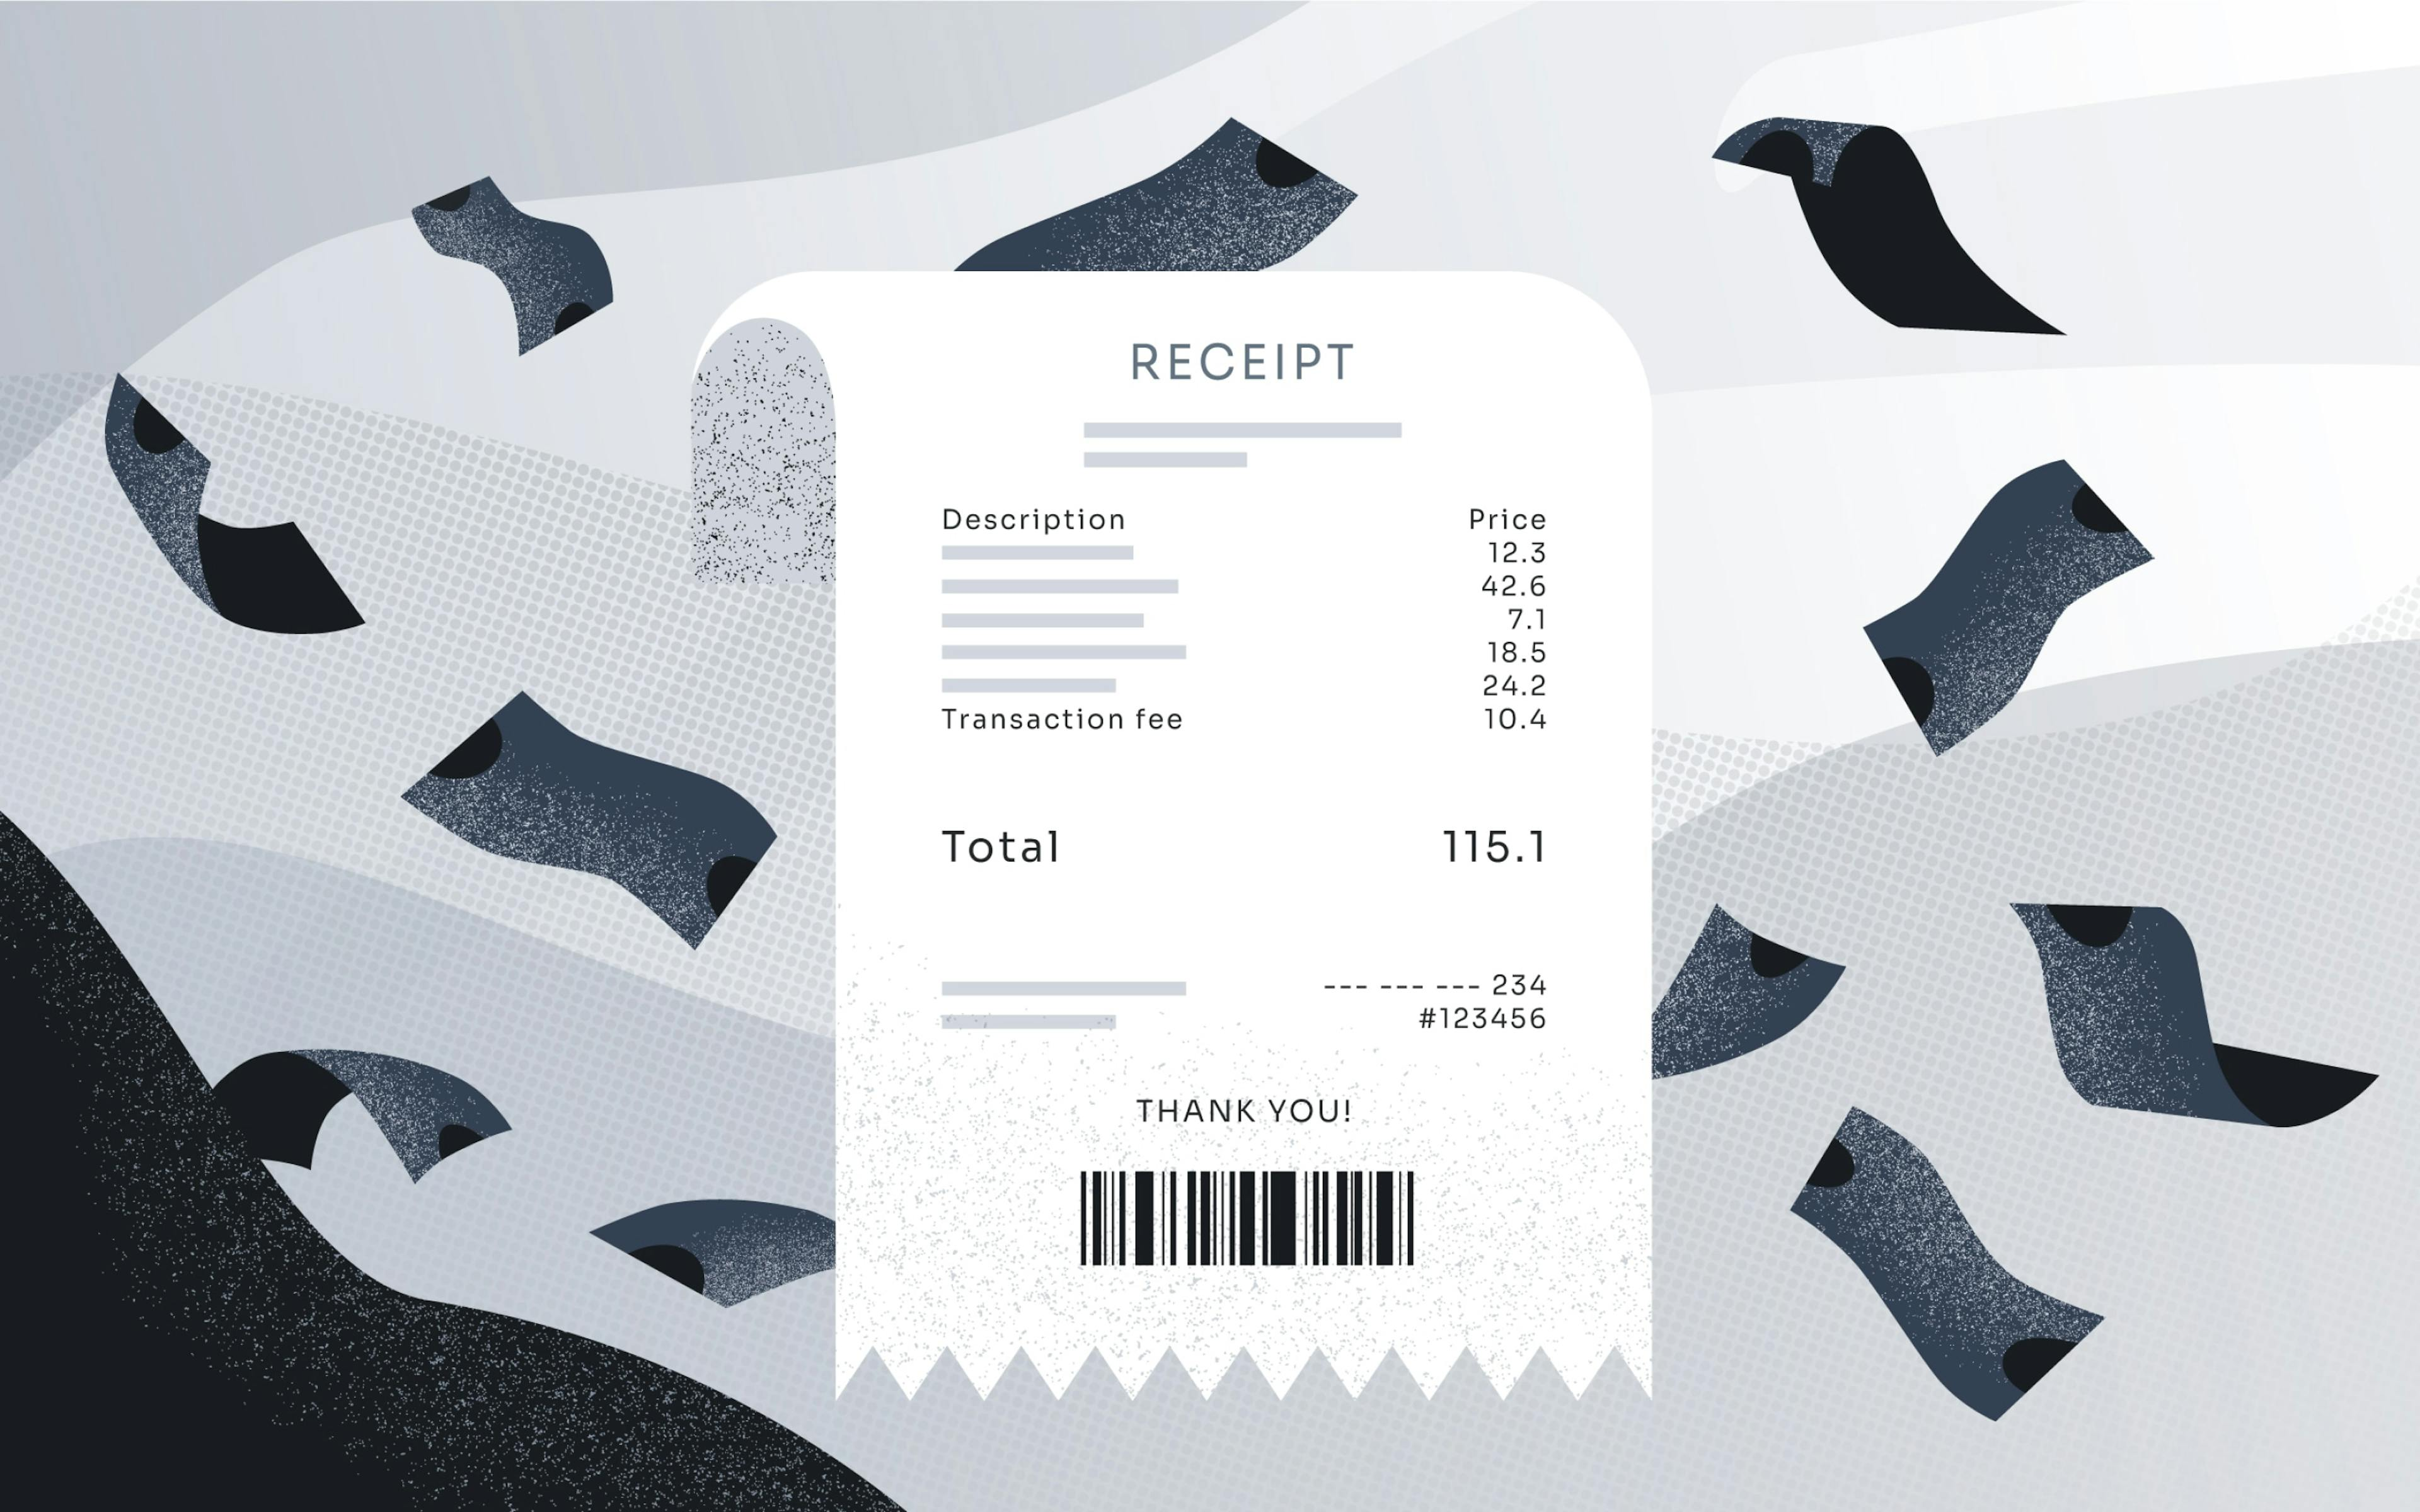
\includegraphics[width=0.5\linewidth]{BSZ_kap_8_2026/by_slide/slide_003/BSZ_kap_8_2026_slide_003_asset_01_image2.jpeg}
  \caption{Transaksjonskostnader: søk-, forhandlings- og håndhevingskostnader som gjør kontrakter ufullstendige -- grunnlaget for costly contracting i Q04. (BSZ kap.\ 8, slide 3) [SLIDE]}
\end{figure}

\begin{figure}[h]
  \centering
  
\includegraphics[width=0.7\linewidth]{BSZ_kap_10_2026/by_slide/slide_005/BSZ_kap_10_2026_slide_005_asset_01_image2.png}
  \caption{Virksomheten som en \emph{nexus of contracts} -- kontrakter mellom eiere, ledere, ansatte, leverandører, kunder, banker. Q04 fokuserer på principal-agent-kontrakten mellom to virksomheter under costly contracting. [SLIDE -- BSZ kap. 10, slide 5]}
\end{figure}

\begin{center}
\renewcommand{\arraystretch}{1.15}
\begin{tabular}{@{}p{3.6cm}p{3.6cm}p{6.5cm}@{}}
\toprule
\textbf{Problem} & \textbf{Tidspunkt} & \textbf{Hovedløsning} \\
\midrule
Adverse selection & Før kontrakt (skjult type) & Signaling, screening, due-diligence, reputasjon \\
Moral hazard & Etter kontrakt (skjult handling) & Monitoring, bonding, insentivkontrakt ($\beta$) \\
Residual loss & Alltid & Aksepteres -- second-best \\
\bottomrule
\end{tabular}
\end{center}
\textit{Tabell: Pre- vs.\ post-kontraktuelle problemer og hvordan de håndteres. [SLIDE]}

\subsection*{Kontrakter under costly contracting og asymmetrisk informasjon -- kort}
\begin{itemize}\setlength{\itemsep}{2pt}
\item \textbf{Pre-kontraktuelt (adverse selection).} Kjøperen (prinsipal) kan ikke skille gode og dårlige tilbydere. Verktøy: due-diligence, sertifisering, garantier, kontraktsmenyer (screening), reputasjon, prøvebestillinger. [SLIDE]
\item \textbf{Post-kontraktuelt (moral hazard).} Etter signering kan agenten redusere kvalitet/innsats skjult. Verktøy: milepælsbetaling, performance bonds, monitoring/revisjon, insentivkontrakter ($W = W_0 + \beta Q$), claw-back, vertikal integrasjon ved særlig hold-up-risiko. [SLIDE]
\item \textbf{Residual control.} Når kontrakten er ufullstendig (begrenset rasjonalitet), er det den som eier aktiva som bestemmer i uregulerte tilstander -- begrunnelsen for vertikal integrasjon. [BOK]
\item \textbf{Trade-off:} Optimal $\beta$ balanserer motivasjon mot risikopremie pluss monitoring/bonding-kostnader. Resultatet er second-best, ikke first-best. [SLIDE]
\end{itemize}

\subsection*{Fordele og ulemper ved kontraktsmekanismene}
\begin{itemize}\setlength{\itemsep}{2pt}
\item \textbf{Due-diligence / screening.} Fordel: avdekker skjult type før kontrakt; reduserer adverse selection. Ulempe: kostbart, gir bare punktestimat, kan ikke fange dynamiske endringer; risiko for ``vinnerens forbannelse'' der den som vinner budet er den som overvurderer mest. [SLIDE]
\item \textbf{Signaling (garantier, sertifisering, eierandel).} Fordel: informert part forplikter seg på troverdig vis (separating equilibrium). Ulempe: signalet er kostbart for høye-typer også; svake typer kan etterligne hvis kostnaden ikke er separerende nok. [SLIDE]
\item \textbf{Monitoring.} Fordel: gjør skjult handling observerbar etter kontrakt; reduserer moral hazard. Ulempe: direkte kostnad pluss demotiverende mikroledelse; måler ofte input, ikke output, og trigger gaming. [SLIDE]
\item \textbf{Bonding (skin-in-the-game, vesting, claw-back).} Fordel: agenten internaliserer prinsipalens risiko -- selvbinding er billigere enn ekstern overvåkning. Ulempe: krever at agenten har formue å binde, og overfører risiko til typisk risikoavers part (krever risikopremie). [BOK]
\item \textbf{Insentivkontrakt ($W = W_0 + \beta Q$).} Fordel: lineær mekanisme som er enkel å forstå og håndheve. Ulempe: når $Q$ inneholder mye støy, blir nødvendig $\beta$ liten -- svake insentiver er det beste man kan oppnå. [SLIDE]
\item \textbf{Vertikal integrasjon / residual control.} Fordel: eierskap allokerer beslutningsrett i uregulerte tilstander; løser hold-up når aktivaspesifisitet er høy. Ulempe: bytter markedsdisiplin mot intern byråkrati og svake insentiver i den integrerte enheten. [BOK -- BSZ kap. 19]
\end{itemize}

\subsection*{Forutsetninger for valg av mekanisme}
\begin{itemize}\setlength{\itemsep}{2pt}
\item \textbf{Adverse selection dominerer} (typeusikkerhet er hovedproblemet): screening og signaling først; gjentatte transaksjoner gir reputasjonsverdi.
\item \textbf{Moral hazard dominerer} (handlingen er hovedproblemet): monitoring + variabel $\beta$ + bonding; jo mer presis $Q$-måling, desto høyere $\beta$.
\item \textbf{Begge til stede} (typisk virkelighet): kombiner screening (forkant) + insentivkontrakt (etterkant); designvalget styres av relative kostnader.
\item \textbf{Aktivaspesifisitet er høy + kontrakt er ufullstendig:} integrer vertikalt; bytt eksterne insentiver mot interne residuelle rettigheter.
\item \textbf{Agenten er svært risikoavers eller fattig:} reduser $\beta$, øk $W_0$, fokuser på monitoring i stedet for bonding.
\end{itemize}

\subsection*{Real-world eksempler}

\textbf{Eks.~1 -- Statoil--Hydro-fusjonen (2007), adverse selection.}\quad [EKS]
To store norske virksomheter med privat informasjon om egne reserver, kontrakter og forpliktelser måtte gjennom flere måneder med due-diligence (klassisk screening) og uavhengige verifikasjoner (signaling) før bytteforholdet kunne fastsettes. Selv etter dette viste integrasjonen flere ``overraskelser'' -- typiske residual losses fra ikke fullstendig løst pre-kontraktuell informasjonsasymmetri.

\textbf{Eks.~2 -- DNB rådgiverprovisjoner (2010-tallet), moral hazard -- sammenligning.}\quad [EKS]
DNB-rådgivere fikk provisjon for å selge bankens egne fond. Atferden var skjult både for kunde og toppledelse, og rådgiverne valgte produkter med høyere kostnad enn nødvendig -- klassisk post-kontraktuell moral hazard. Forbrukerrådets shadow shopping (monitoring) avslørte forholdet og førte til at provisjonsmodellen ble fjernet (regulatorisk endring av $\beta$-strukturen). Sammenligning med Statoil-Hydro: samme principal-agent-rammeverk, men problemet er på \emph{ulike sider} av kontraktinngåelsen -- adverse selection vs.\ moral hazard. Løsningsverktøyene er derfor ulike: due-diligence og signaling i forkant vs.\ monitoring og endret insentivkontrakt i etterkant.

\subsection*{Kobling til Mærsk Power-to-X}
Mærsks Power-to-X-satsing er et lærebok-eksempel på begge problemene under costly contracting mellom \emph{to virksomheter}. \emph{Adverse selection}: ved valg av teknologipartner (elektrolyseleverandør, hydrogenkjøper) kjenner partneren sin egen reelle modenhet og kostnadsstruktur bedre enn Mærsk -- løses med teknisk due-diligence, krav om referanseprosjekter (signaling) og garantier. \emph{Moral hazard}: etter kontraktinngåelse kan en EPC-kontraktør skjule fremdriftsproblemer eller kvalitetskutt -- løses med milepælsbetaling, on-site supervision (monitoring), performance bonds (bonding) og deling av oppside via partnerskap (variabel $\beta$). Når kontrakten ikke kan dekke alle fremtidige tilstander (teknologi-, regulatorisk- og prisrisiko), kan Mærsk velge vertikal integrasjon på de mest spesifikke aktivaene. [CASE]

\subsection*{Fallgruber}
\begin{itemize}\setlength{\itemsep}{2pt}
\item Ikke gjenta Q03 -- her er hele poenget at \emph{forutsetningene} er andre (costly + asymmetrisk).
\item Forveksle adverse selection og moral hazard -- nøkkelen er \emph{tidspunkt} og \emph{type skjult variabel} (egenskap vs.\ handling).
\item Glemme residual loss -- selv optimal kontrakt etterlater et tap.
\item Hoppe over to-virksomhets-rammen -- spørsmålet ber eksplisitt om interfirm-kontekst.
\item Gi inntrykk av at kontrakten kan ``løse'' problemet -- under costly contracting reduseres det, ikke elimineres.
\item Glemme at signaling og screening er to forskjellige svar (informert part vs.\ uinformert part tar grep).
\end{itemize}

\subsection*{Håndskrivbar disposisjon (15-min forberedelse)}
\begin{itemize}\setlength{\itemsep}{2pt}
\item \textbf{Tese:} Samme 5 konflikter som Q03, men under costly contracting + asymmetrisk info kan kontrakten ikke eliminere dem -- kun second-best.
\item Virksomheten = \emph{nexus of contracts}; her ser vi på principal-agent-kontrakten mellom \emph{to virksomheter}.
\item \thref{incentive-conflicts-owner-manager}{5 konflikter}: shirking, perks, risikoaversjon, tidshorisont, overinvestering.
\item \thref{costly-contracting}{Costly contracting}: search/forhandling/drafting/monitoring/enforcement -- kontrakten blir ufullstendig.
\item \thref{adverse-selection}{Adverse selection} = pre-kontraktuell, skjult \emph{type} $\Rightarrow$ signaling (informert part) + screening / due-diligence (uinformert part).
\item \thref{moral-hazard}{Moral hazard} = post-kontraktuell, skjult \emph{handling} $\Rightarrow$ monitoring + bonding + insentivkontrakt ($\beta > 0$).
\item \thref{principal-agent}{Principal-agent}-modellen $W = W_0 + \beta Q$: optimal $\beta$ balanserer motivasjon mot risikopremie + agency cost.
\item Residual loss $+$ monitoring $+$ bonding = \thref{agency-costs}{agency costs}; transaksjonen kan falle vekk hvis disse blir for store.
\item Eks. 1: Statoil-Hydro 2007 -- adverse selection, due-diligence.
\item Eks. 2: DNB rådgiverprovisjoner -- moral hazard, monitoring + regulatorisk endring av $\beta$.
\item Mærsk Power-to-X: teknologipartner = adverse selection; EPC-kontraktør = moral hazard; ufullstendig kontrakt $\Rightarrow$ vertikal integrasjon for kjerneaktiva.
\item Kontrast Q03: der \thref{costless-contracting}{costless contracting} = first-best; her costly + asymmetrisk = second-best.
\item Søyle: \SThree\ primært, også \SOne\ (residual control rights).
\end{itemize}

% !TEX root = ../main.tex
\section{Q05: Agentomkostninger, viden, insentiver -- og arkitekturens tre ben}\label{q:05}

\begin{quote}
\emph{På baggrund af en redegørelse for begreberne: a) agentomkostninger, b) specifik og generel viden, c) incitamenter, forklares hvilke problemer økonomisk organisationsteori (arkitektur) angiver at kunne løse og på hvilken måde. De enkelte ``ben'' i arkitekturen forventes forklaret specifikt i denne sammenhæng og gerne understøttet af gennemgåede cases og/eller opgaver.}
\end{quote}

\subsection*{Svar (kort)}
Økonomisk organisasjonsteori (BSZ kap.\ 11) løser to grunnproblemer som oppstår når informasjon er distribuert (Hayek) og ansatte har egne preferanser (Jensen \& Meckling): et \emph{informasjonsproblem} -- hvem skal beslutte når \thref{specific-vs-general-knowledge}{spesifik viden} sitter lokalt -- og et \emph{insentivproblem} -- hvordan får man agenten til å velge i prinsipalens interesse, slik at \thref{agency-costs}{agentomkostningene} (monitoring + bonding + residual loss) minimeres. Løsningen er den tre-benede skammelen \thref{organizational-architecture}{organizational architecture}: beslutningsrettigheter (S1), prestasjonsmåling (S2) og insentivstruktur (S3) må designes \emph{samtidig} og som komplementer -- endrer man ett ben uten de andre, faller skammelen og residual loss eksploderer. [SLIDE]

\subsection*{Begrepene (kort)}

\paragraph{a) \thref{agency-costs}{Agentomkostninger}\quad\SOne/\STwo/\SThree}
Verditapen som oppstår fordi agenten ikke handler fullt ut i prinsipalens interesse. Jensen \& Meckling (1976) deler den i tre: \emph{monitoring} (prinsipalens overvåkingsutgift), \emph{bonding} (agentens troverdighetssignaler, f.eks.\ opsjoner, covenants) og \emph{residual loss} (gjenværende effektivitetstap). Optimalt designes M og B for å minimere \emph{summen} -- residual loss fjernes ikke helt fordi det er for dyrt. Hele arkitekturen finnes for å minimere agentomkostninger. [SLIDE]

\paragraph{b) \thref{specific-vs-general-knowledge}{Spesifik vs.\ generell viden}\quad\SOne}
Spesifik viden er kostbar å overføre (lokal, taus, tidssensitiv); generell viden er billig (kvantifiserbar, kodifisert). Hayek (1945): viktig viden er distribuert. Jensen \& Meckling (1992): organisasjonen må enten \emph{flytte videnen til beslutningen} (sentralisere + informasjonsflyt) eller \emph{flytte beslutningen til videnen} (desentralisere + agentstyring). Spesifik viden $\Rightarrow$ desentralisering $\Rightarrow$ men da kreves S2 og S3 for å erstatte tapt direkte kontroll. Dette er det driveren som kobler S1 til S2/S3. [SLIDE/BOK]

\paragraph{c) Incitamenter\quad\SThree}
\emph{Insentiver} er mekanismer som vrir agentens egennytte mot prinsipalens mål -- prestasjonslønn, bonus, opsjoner, karriereutvikling, status, anerkjennelse. Insentiver virker bare når (i) prestasjon kan måles meningsfullt (S2), (ii) lederen har beslutningsrett over det hun måles på (S1, jf.\ \thref{controllability-principle}{controllability}), og (iii) målene er informative om innsats (jf.\ \thref{informativeness-principle}{informativeness}). Sterke insentiver overfører risiko til en (typisk) risikoavers agent -- løsningen koster derfor en risikopremie. Insentivvalget er det tredje benet i skammelen. [SLIDE]

\subsection*{De tre benene -- hva hver gjør, og hvorfor de er komplementer}

\begin{center}
\renewcommand{\arraystretch}{1.15}
\begin{tabular}{@{}p{2.7cm}p{4.6cm}p{6.6cm}@{}}
\toprule
\textbf{Søyle / ben} & \textbf{Designvariabel} & \textbf{Hva benet gjør} \\
\midrule
\SOne\ Decision rights & Allokering av beslutningsmakt & Plasserer beslutningen der \emph{spesifik viden} sitter; reduserer informasjonsproblemet. \\
\STwo\ Performance eval. & Hva som måles og hvordan & Erstatter direkte observasjon når desentralisering velges; må være kontrollerbart og informativt. \\
\SThree\ Reward system & Lønn, bonus, opsjoner, karriere & Vri agentens egennytte mot prinsipalens mål; balanserer insentiv mot risikodeling. \\
\bottomrule
\end{tabular}
\end{center}

\textbf{Hvorfor komplementer?} Marginalavkastningen av ett ben stiger med kvaliteten på de to andre. Misalignment-eksempler:
\begin{itemize}\setlength{\itemsep}{2pt}
\item Desentralisering (S1) uten måltall (S2) $\Rightarrow$ kontroll uten ansvar; residual loss eksploderer.
\item Aksjebasert bonus (S3) uten meningsfullt måltall (S2) $\Rightarrow$ ledelsen belønnes for makroflaks (gaming).
\item Skarp måling (S2) uten beslutningsrett (S1) $\Rightarrow$ bryter \thref{controllability-principle}{controllability}; demotiverende.
\item Insentiv (S3) uten beslutningsrett (S1) $\Rightarrow$ agenten kan ikke handle på det.
\end{itemize}

\subsection*{Hvilke problemer løses og hvordan?}
\begin{enumerate}\setlength{\itemsep}{2pt}
\item \textbf{Informasjonsproblem} (spesifik viden er distribuert). Løses ved S1: flytt beslutningsretten dit videnen er.
\item \textbf{Insentivproblem} (agenten har egne preferanser). Løses ved S3 koblet til S2: gjør det lønnsomt for agenten å velge prinsipalens optimum.
\item \textbf{Koordinasjonsproblem} (mange aktører, potensielle eksternaliteter). Løses ved S1+S2 sammen: ansvarsenheter (\thref{responsibility-centers}{responsibility centers}) med klare grensesnitt og evt.\ \thref{transfer-pricing}{transfer pricing} mellom dem.
\item \textbf{Kontrollproblem} (decentralisering åpner for opportunisme). Løses ved monitoring (S2) + bonding via insentiv (S3) -- minimum av agentomkostninger gitt at residual loss aksepteres.
\item \textbf{Tilpasningsproblem} (endrede omgivelser). Løses ved at arkitekturen tilpasses så lenge MR $>$ MC; firmaer som ikke endrer seg, rammes av \emph{economic Darwinism}.
\end{enumerate}

\subsection*{Illustrasjon}

\begin{figure}[h]
  \centering
  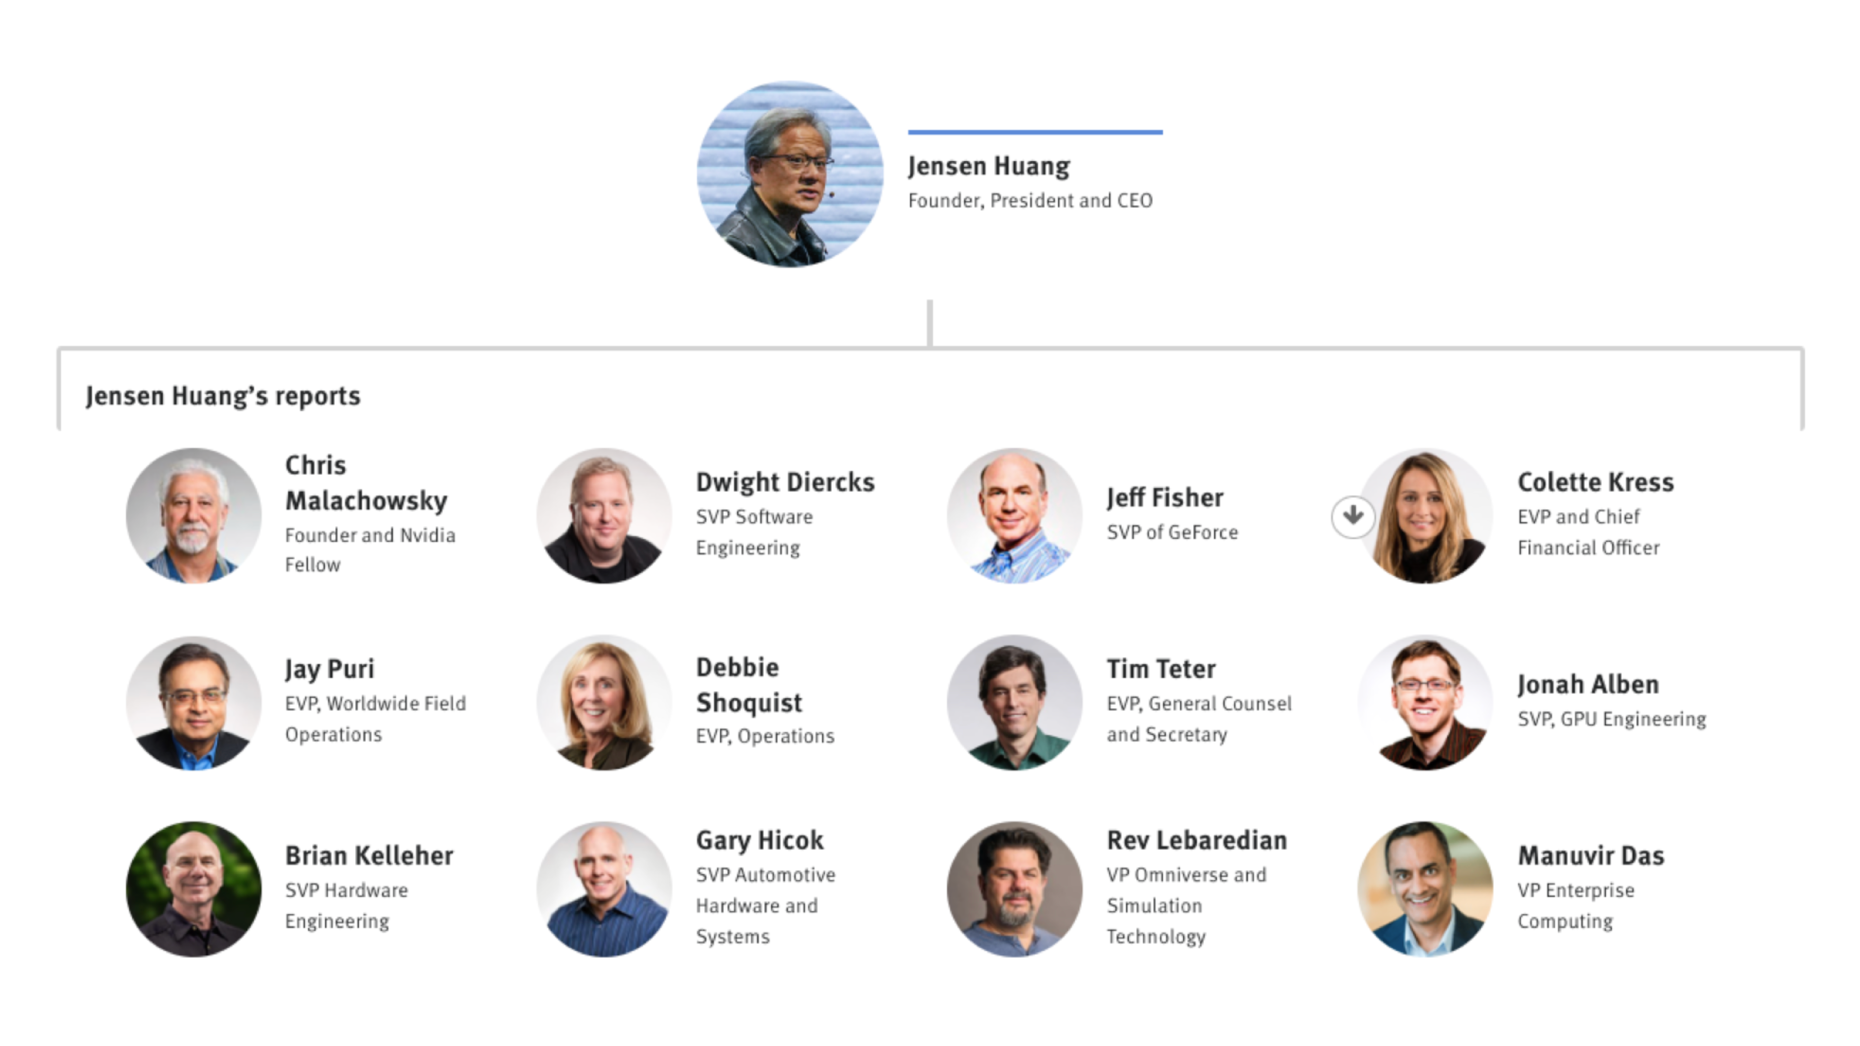
\includegraphics[width=0.65\linewidth]{BSZ_kap_11_2026/by_slide/slide_004/BSZ_kap_11_2026_slide_004_asset_01_image3.png}
  \caption{Den tre-benede skammelen: Decision rights, Performance evaluation, Reward systems -- arkitekturens tre ben må designes samtidig. (BSZ kap.\ 11, slide 4) [SLIDE]}
\end{figure}

\begin{figure}[h]
  \centering
  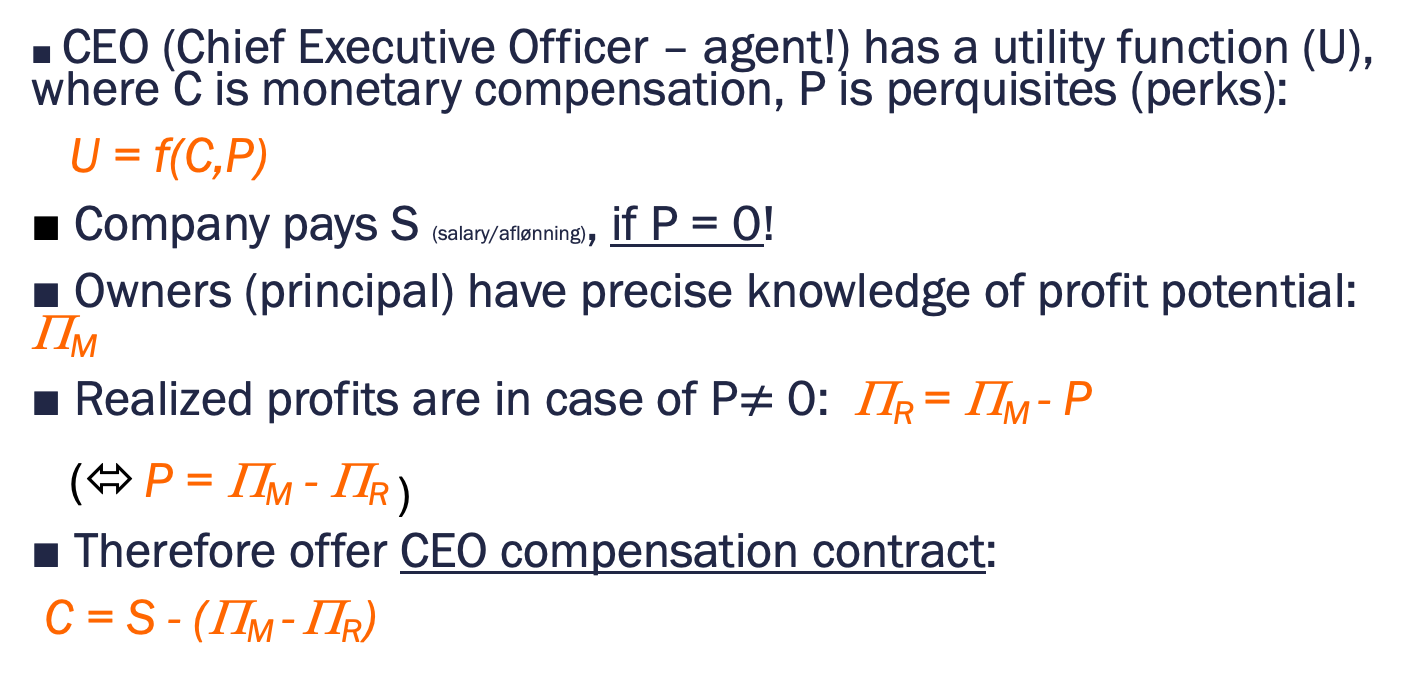
\includegraphics[width=0.55\linewidth]{BSZ_kap_10_2026/by_slide/slide_007/BSZ_kap_10_2026_slide_007_asset_01_image3.png}
  \caption{Agency cost-dekomponering: monitoring + bonding + residual loss reduserer first-best-verdien av en handel. (BSZ kap.\ 10, slide 7) [SLIDE]}
\end{figure}

\subsection*{Real-world eksempler}

\textbf{Eks.~1 -- Equinor (omorganisering 2020/2021).}\quad [EKS]
Da Equinor besluttet å bygge ut fornybar virksomhet betydelig, ble \emph{Renewables} skilt ut som egen forretningsenhet med eget lederskap (S1: ny beslutningsstruktur), separate KPI-er for fornybar kapasitet og avkastning (S2: tilpasset prestasjonsmåling) og ledelseskompensasjon koblet til transisjonsmål (S3: nye insentiver). Hadde Equinor bare flyttet beslutningsrett uten å endre måltall (fortsatt målt på olje-EBITDA), ville fornybarsatsingen kollapset -- klassisk misalignment.

\textbf{Eks.~2 -- Norsk Hydro vs.\ Equinor (sammenligning).}\quad [EKS]
Norsk Hydro driver vertikalt integrert aluminiumsproduksjon med separate divisjoner (Bauxite \& Alumina, Aluminium Metal, Extruded Solutions). Hver divisjon er investment center (S1), måles på LME-justert margin (S2 -- jf.\ \thref{controllability-principle}{controllability}-prinsippet), og bonus er knyttet til divisjonsresultat (S3). Sammenlignet med Equinor: \emph{samme prinsipp om å designe alle tre ben samtidig}, men i Hydro driver \emph{teknologi og prismekanismen for råvarer} arkitekturen, mens i Equinor er det \emph{strategisk transisjon}. Begge viser at den tre-benede skammelen er anvendbar uavhengig av bransje.

\subsection*{Kobling til Mærsk Power-to-X}
PtX-divisjonens arkitektur er et lærebokeksempel på de tre benene i sammenheng: [CASE]
\begin{itemize}\setlength{\itemsep}{2pt}
\item \SOne\ \emph{Decision rights:} Beslutningsrett om elektrolysørteknologi og partnervalg er delegert ned til PtX-divisjonen, fordi den \thref{specific-vs-general-knowledge}{spesifikke videnen} om kjemi, prosess og partner-økosystem sitter der -- ikke i konsernledelsen.
\item \STwo\ \emph{Performance evaluation:} Divisjonen drives som \thref{responsibility-centers}{investment center}; måltallet er prosjektets risikojusterte NPV/IRR. Kortsiktig EBITDA-måling ville rammet langsiktige CAPEX-beslutninger og bryte controllability (oljepris- og elprisbevegelser er ikke kontrollerbare).
\item \SThree\ \emph{Reward system:} Lederkompensasjon koblet til langsiktige milestones (anlegg ferdigstilt, kontrakter signert, IRR-måltall) -- bonding via langsiktig egenkapitalandel reduserer agentomkostninger.
\end{itemize}
\textbf{Misalignment-tankeeksperiment:} Hvis ledelsen i PtX hadde fått beslutningsrett (S1) og kompensasjon basert på årets EBITDA (S3), uten et investeringsfølsomt måltall (S2), ville hun utsatt eller skalert ned investeringene -- et klassisk eksempel på horisontproblem og misalignment mellom de tre benene. Caset viser hvorfor alle tre må designes samtidig.

\subsection*{Fallgruber}
\begin{itemize}\setlength{\itemsep}{2pt}
\item Bare nevne ett eller to ben -- sensor venter at alle tre presenteres eksplisitt og kobles til S1/S2/S3.
\item Glemme \emph{komplementaritet} -- poenget er at de tre må endres samtidig.
\item Forveksle bonding med monitoring -- bonding er agentens egen kostnad, monitoring er prinsipalens.
\item Glemme at residual loss er igjen \emph{etter} optimal monitoring og bonding -- den fjernes ikke helt.
\item Behandle ``incitamenter'' som synonymt med ``bonus''. Insentiver inkluderer karriere, status, opsjoner, eierandel, jobbdesign.
\item Ikke knytte spesifik/generell viden til \emph{begrunnelsen} for desentralisering (S1) -- dette er linken Hayek$\to$Jensen\&Meckling.
\item Glemme caset -- spørsmålet inviterer eksplisitt til å bruke gjennomgåtte cases.
\end{itemize}

\subsection*{Håndskrivbar disposisjon (15-min forberedelse)}
\begin{itemize}\setlength{\itemsep}{2pt}
\item \textbf{Tese:} Arkitektur = tre-benet skammel (S1+S2+S3 designet samtidig); løser informasjons- og insentivproblem ved å minimere agentomkostninger.
\item \textbf{Begrep a -- \thref{agency-costs}{Agentomkostninger}:} Monitoring + Bonding + Residual loss (Jensen \& Meckling 1976). Tallregneksempel fra slide 31 kap.\ 10. Aksepter residual loss -- billigere enn perfekt kontroll.
\item \textbf{Begrep b -- \thref{specific-vs-general-knowledge}{Spesifik vs.\ generell viden}:} Hayek $\to$ Jensen \& Meckling. Spesifik viden $\Rightarrow$ desentraliser (flytt beslutning) $\Rightarrow$ men da kreves S2 + S3.
\item \textbf{Begrep c -- Incitamenter:} Vri egennytte mot prinsipal. Krever målbarhet (S2), kontrollerbarhet (S1), informativeness. Risk-incentive trade-off.
\item \textbf{De tre benene:} S1 Decision rights / S2 Performance eval. / S3 Reward. \emph{Komplementer} $\Rightarrow$ misalignment hvis ett endres alene.
\item \textbf{Hvilke problemer løses?} (i) informasjonsproblem (S1), (ii) insentivproblem (S2+S3), (iii) koordinasjon (S1+S2), (iv) kontroll (S2+S3 minimerer agency cost), (v) tilpasning (MR$>$MC, economic Darwinism).
\item \textbf{Eks.\ 1:} Equinor Renewables-utskillelse 2020/2021 -- alle tre ben endret samtidig.
\item \textbf{Eks.\ 2:} Norsk Hydro aluminiumsdivisjoner -- LME-justert måling (controllability) + investment-center-design.
\item \textbf{Case:} Mærsk PtX som investment center -- viser hvorfor alle tre ben må designes sammen; misalignment-tankeeksperiment.
\item \textbf{Søyle:} \SOne\ + \STwo\ + \SThree\ -- spørsmålet spenner alle tre.
\end{itemize}

% !TEX root = ../main.tex
% NB til orchestrator: Denne filen bruker TikZ-figurer i theory-filen optimal-decentralization-model.tex.
% Preamble må utvides med \usepackage{tikz}. Hvis tikz ikke legges til, vil bygget feile på de to TikZ-blokkene i den teorifilen.
% Q06 selv bruker kun \includegraphics og er ikke avhengig av tikz.
\section{Q06: Centralisering vs.\ decentralisering -- trade-offs og optimal grad}\label{q:06}

\begin{quote}
\emph{Redegør for fordele og ulemper ved samt trade-offs mellem centralisering og decentralisering. Præsentér herefter kriterier for fastlæggelse af optimal decentraliseringsgrad og redegør specifikt grafisk for modellen til illustration heraf.}
\end{quote}

\subsection*{Svar (kort)}
\thref{centralization-vs-decentralization}{Sentralisering vs.\ desentralisering} er et \emph{kontinuum} -- en glidende skala, ikke et binært valg. Desentralisering utnytter \thref{specific-vs-general-knowledge}{spesifik lokal viden} (kunnskap som er kostbar å overføre oppover, jf.\ Hayek; Jensen \& Meckling), men introduserer \thref{agency-costs}{agentomkostninger} (kostnaden ved at lokal leder kan handle i egen interesse) og koordineringskostnader. Optimal grad $D^{*}$ ligger der marginal fordel av lokal viden møter marginal kostnad av agent- og koordineringsproblemer. BSZ-modellen (kap.\ 12) gir nettogevinst $\mathrm{NB}(D) = BD - AD - CD^{2}$, dvs.\ desentraliseringsgraden $D$ ganger nytte minus kostnader; jo mer du desentraliserer, jo mer lokal viden ($BD$) -- men også jo mer agentkostnad ($AD$) og en koordineringskostnad som vokser kvadratisk ($CD^{2}$). Optimum er $D^{*} = (B-A)/(2C)$. Tolkning: jo høyere nytten $B$ av lokal viden, jo høyere optimal desentralisering; jo høyere agent- og koordineringskostnad ($A$ og $C$), jo mindre desentralisering. Hver gang beslutningsrettighetene (\SOne) flyttes, må prestasjonsmåling (\STwo) og insentiver (\SThree) justeres med, ellers faller arkitekturen. [SLIDE/BOK]

\subsection*{Fordele og ulemper (kort)}

\begin{center}
\renewcommand{\arraystretch}{1.15}
\begin{tabular}{@{}p{2.5cm}p{6.0cm}p{6.0cm}@{}}
\toprule
& \textbf{Sentralisering} & \textbf{Desentralisering} \\
\midrule
\textbf{Fordele} & Koordinering, stordrift, konsistens, lave agentkostnader & Lokal viden, hurtighet, motivasjon/ledertrening, avlastning av toppledelse \\
\textbf{Ulemper} & Tap av lokal viden, treghet, toppledelsesoverload, demotivasjon nede & Agentkostnader, koordineringssvikt, tap av stordrift, inkonsistente beslutninger \\
\bottomrule
\end{tabular}
\end{center}
\emph{Trade-off i én linje:} Desentralisering gir bedre informasjon men dårligere insentivlinje; sentralisering gir bedre insentivlinje men dårligere informasjon. [SLIDE]

\subsection*{Relevante teorier (kort)}

\paragraph{\thref{centralization-vs-decentralization}{Centralisering vs.\ desentralisering}\quad\SOne}
Beslutningsrett kan plasseres høyt (CEO/konsern) eller delegeres nedover. Valget er det første benet i arkitekturen og det drives av om videnen som trengs til beslutningen er spesifik eller generell. I praksis blandes sentralisering og desentralisering på ulike beslutningsklasser -- f.eks.\ kapitalallokering sentralt, daglig drift lokalt. [SLIDE/BOK]

\paragraph{\thref{optimal-decentralization-model}{Optimal desentraliseringsgrad}\quad\SOne}
BSZ-modellen formaliserer trade-off-en: $\mathrm{NB}(D) = B \cdot D - A \cdot D - C \cdot D^{2}$ med optimum $D^{*} = (B-A)/(2C)$, der $B$ er marginal nytte av lokal viden (gevinst per ekstra desentraliseringssteg), $A$ er marginal agentkostnad og $C$ er konveks koordineringskostnad. Setter man derivatet lik null får man $B - A - 2CD = 0$, og løser for $D^{*}$. \emph{Komparativ statikk} -- altså hvordan optimum endres med parametrene: $\partial D^{*}/\partial B > 0$ (mer verdifull lokal viden $\Rightarrow$ mer desentralisering), $\partial D^{*}/\partial A < 0$ (større agentkostnad $\Rightarrow$ mindre desentralisering), $\partial D^{*}/\partial C < 0$ (større koordineringskostnad $\Rightarrow$ mindre desentralisering). [SLIDE]

\paragraph{\thref{specific-vs-general-knowledge}{Spesifik vs.\ generell viden}\quad\SOne}
Hayek (1945) og Jensen \& Meckling (1992): viden er distribuert. Spesifik viden er kostbar å overføre $\Rightarrow$ flytt \emph{beslutningen} til videnen (desentraliser). Generell viden er billig $\Rightarrow$ flytt \emph{videnen} til beslutningen (sentraliser). Dette er driveren for $B$ i modellen -- og forklarer hvorfor IT-revolusjonen kan re-sentralisere når tidligere spesifik viden kodifiseres. [SLIDE/BOK]

\paragraph{\thref{agency-costs}{Agentomkostninger}\quad\SOne/\STwo/\SThree}
Når beslutningsretten flyttes nedover, mister prinsipalen direkte kontroll. Jensen \& Meckling dekomponerer agentkostnaden: $\text{AC} = \text{monitoring} + \text{bonding} + \text{residual loss}$ -- altså summen av prinsipalens overvåkningsutgifter (monitoring), agentens egne forpliktelsessignaler som covenants og opsjoner (bonding), og det effektivitetstapet som likevel gjenstår (residual loss). Modellens $A$-parameter er nettopp marginal agentkostnad ved økt desentralisering. Den minimeres ved samtidig å designe \STwo\ (hva som måles) og \SThree\ (hvordan agenten belønnes) som erstatter den tapte kontrollen. Endrer man bare \SOne\ uten å justere S2/S3, eksploderer $A$ og $D^{*}$ trekkes mot null. [BOK]

\subsection*{Illustrasjoner fra forelesning}

\begin{figure}[H]
  \centering
  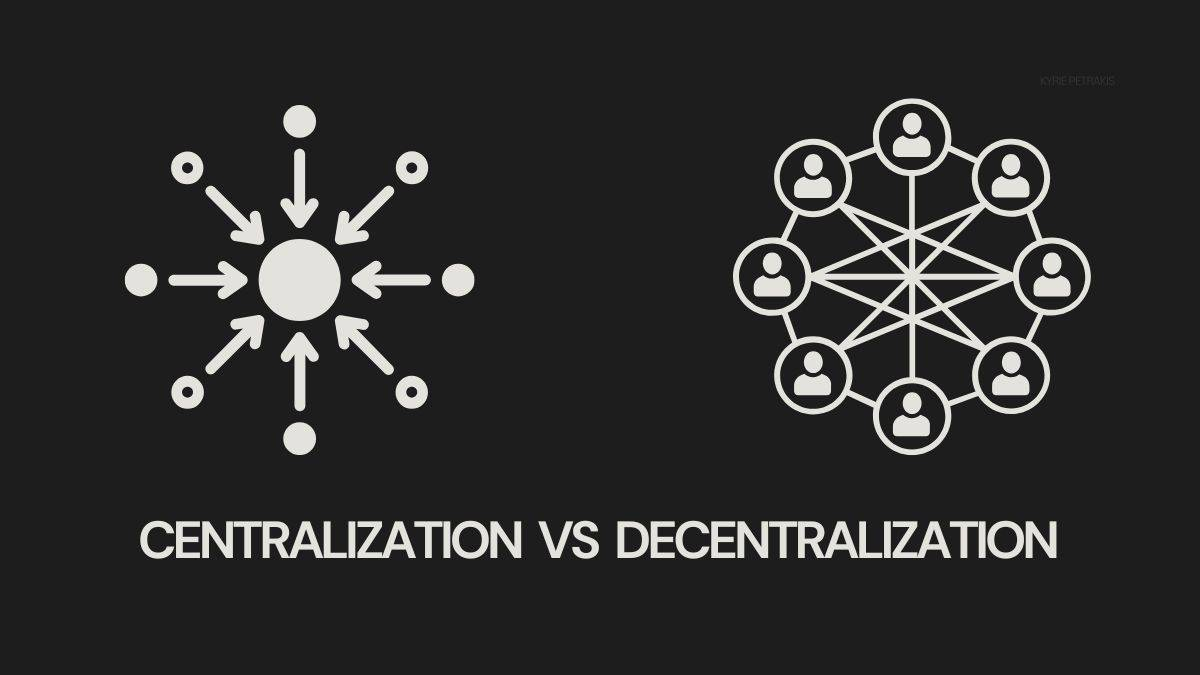
\includegraphics[width=0.6\linewidth]{BSZ_kap_12_2026/by_slide/slide_004/BSZ_kap_12_2026_slide_004_asset_01_image1.jpeg}
  \caption{Sentralisering vs.\ desentralisering -- trade-off mellom lokal viden og kontroll. (BSZ kap.\ 12, slide 4) [SLIDE]}
\end{figure}

\begin{figure}[H]
  \centering
  
\includegraphics[width=0.6\linewidth]{BSZ_kap_12_2026/by_slide/slide_018/BSZ_kap_12_2026_slide_018_asset_01_image6.jpeg}
  \caption{Spesifik viden og kommunikasjon -- hvorfor desentralisering kreves når viden er kostbar å overføre. (BSZ kap.\ 12, slide 18) [SLIDE]}
\end{figure}

\subsection*{Grafisk modell (obligatorisk)}

\paragraph{Fra totalnivå til marginalnivå -- utledning av $D^{*}$.}
Modellen opererer på to nivåer. Først definerer vi \emph{totalkurvene}:
\[
  \mathrm{TB}(D) = B \cdot D \qquad \text{(total fordel -- lineær i $D$)}
\]
\[
  \mathrm{TC}(D) = A \cdot D + C \cdot D^{2} \qquad \text{(total kostnad -- konveks i $D$)}
\]
Nettofordel er differansen mellom total fordel og total kostnad:
\[
  \mathrm{NB}(D) \;=\; \mathrm{TB}(D) - \mathrm{TC}(D) \;=\; BD - AD - CD^{2}
\]
For å finne den $D$ som \emph{maksimerer} NB, deriverer vi NB med hensyn på $D$ og setter lik null:
\[
  \frac{d\,\mathrm{NB}}{dD}
  \;=\; \underbrace{\frac{d(\mathrm{TB})}{dD}}_{=\;\mathrm{MB}\,=\,B}
  \;-\; \underbrace{\frac{d(\mathrm{TC})}{dD}}_{=\;\mathrm{MC}\,=\,A+2CD}
  \;=\; B - A - 2CD \;=\; 0
\]
\[
  \boxed{\;D^{*} = \frac{B-A}{2C}\;}
\]
Altså: å derivere $\mathrm{NB}(D)$ og løse for $D$ gir \emph{direkte} $D^{*}$. Og fordi derivatet av TB er MB og derivatet av TC er MC, er betingelsen $d\mathrm{NB}/dD = 0$ \emph{identisk} med betingelsen $\mathrm{MB} = \mathrm{MC}$. Det er to fremstillinger av \emph{samme} optimum.

\paragraph{Geometrisk kobling mellom de to panelene.}
Figuren nedenfor viser begge nivåer:
\begin{itemize}[nosep]
  \item \textbf{Øvre panel (TC/TB):} NB er den \emph{vertikale avstanden} mellom TB og TC. Denne avstanden er størst ved $D^{*}$.
  \item \textbf{Nedre panel (MC/MB):} $D^{*}$ er skjæringspunktet mellom MB og MC.
\end{itemize}
De to panelene er ekvivalente: der totalkurvene har størst avstand, er også der marginalkurvene krysser -- fordi størst avstand betyr at \emph{stigningsratene} (derivatene) er like.

\begin{figure}[H]
\centering
\begin{tikzpicture}[scale=1.0]
  % === ØVRE PANEL: TC og TB (totalkurver) ===
  \begin{scope}[yshift=7.5cm]
    \draw[->, thick] (0,0) -- (7.5,0) node[right] {$D$};
    \draw[->, thick] (0,0) -- (0,7) node[above] {kr (totalt)};
    % TB = BD = 4D, skalert /4 => D
    \draw[thick, blue!70!black, domain=0:6.8, samples=80]
      plot (\x, {\x}) node[right] {$\mathrm{TB}=BD$};
    % TC = AD + CD^2 = D + 0.5D^2, skalert /4 => 0.25D + 0.125D^2
    \draw[thick, red!70!black, domain=0:6.5, samples=80]
      plot (\x, {0.25*\x + 0.125*\x*\x}) node[right] {$\mathrm{TC}=AD+CD^{2}$};
    % D* striplet linje
    \draw[dashed, gray] (3,0) -- (3,3);
    \node[below] at (3,0) {$D^{*}$};
    % Dobbeltpil for max NB ved D*
    \draw[<->, thick, green!60!black] (3,1.875) -- (3,3);
    \node[right, green!60!black, font=\small] at (3.15,2.44) {$\max\;\mathrm{NB}(D^{*})$};
    % Prikk ved break-even D=6 der TB=TC
    \filldraw[black] (6,6) circle (1.5pt);
    \node[above left, font=\footnotesize] at (6,6) {$\mathrm{TB}=\mathrm{TC}$};
    % Prikker på kurvene ved D*
    \filldraw[blue!70!black] (3,3) circle (1.5pt);
    \filldraw[red!70!black] (3,1.875) circle (1.5pt);
  \end{scope}
  % === Forbindelseslinje mellom panelene ===
  \draw[dashed, gray, thin] (3,4) -- (3,7.5);
  % === NEDRE PANEL: MC og MB (marginalkurver) ===
  \draw[->, thick] (0,0) -- (7.5,0) node[right] {$D$};
  \draw[->, thick] (0,0) -- (0,6) node[above] {kr (marginal)};
  % MB = B = 4, konstant
  \draw[thick, blue!70!black] (0,4) -- (7,4) node[right] {$\mathrm{MB}=B$};
  % MC = A + 2CD = 1 + D
  \draw[thick, red!70!black] (0,1) -- (5,6) node[right] {$\mathrm{MC}=A+2CD$};
  % D* striplet linje
  \draw[dashed, gray] (3,0) -- (3,4);
  \filldraw[black] (3,4) circle (1.5pt);
  \node[below] at (3,0) {$D^{*}$};
  \node[left] at (0,4) {$B$};
  \node[left] at (0,1) {$A$};
  \node[above left, font=\small] at (3,4) {$\mathrm{MB}=\mathrm{MC}$};
\end{tikzpicture}
\caption{Øvre panel: totalkurvene TB (lineær) og TC (konveks) -- størst vertikal avstand ved $D^{*}$. Nedre panel: marginalkurvene MB (horisontal) og MC (stigende) -- krysser ved $D^{*}$. Panelene viser \emph{samme} optimum: maks avstand mellom totalkurvene inntreffer \emph{nøyaktig} der marginalkurvene er like. Talleksempel: $B=4,\; A=1,\; C=0{,}5 \;\Rightarrow\; D^{*}=3$. Skifter $B$ opp $\Rightarrow$ $D^{*}$ til høyre; skifter $A$ eller $C$ opp $\Rightarrow$ $D^{*}$ til venstre. [SLIDE/EGEN]}
\end{figure}

\textbf{Leseveiledning for figuren.} Den horisontale aksen $D$ måler grad av desentralisering fra 0 (full sentralisering) mot høyre (mer desentralisering). I det øvre panelet er TB-linjen rett (stigning $B$) og TC-kurven konveks (stigning $A + 2CD$ som øker i $D$); den grønne pilen markerer $\max\mathrm{NB}$, dvs.\ nettofordelen ved $D^{*}$. I det nedre panelet er MB horisontal på $B$ og MC stiger fra $A$ med stigning $2C$; skjæringspunktet er $D^{*}$. Den stiplede linjen viser at $D^{*}$ i begge paneler er \emph{samme} punkt -- dette er kjernen i modellen: \emph{derivert} $\mathrm{NB}$ lik null $\Leftrightarrow$ $\mathrm{MB} = \mathrm{MC}$. En mer detaljert avledning og en alternativ NB-parabel-figur finnes i teorifilen \thref{optimal-decentralization-model}{optimal decentraliseringsmodell}. [SLIDE]

\subsection*{Real-world eksempler}

\textbf{Eks.\ 1 -- Equinor (E\&P vs.\ konsernfinans).}\quad [EKS]
Letevirksomheten i Equinor er sterkt desentralisert til prosjektledere som investment centers fordi den \thref{specific-vs-general-knowledge}{spesifikke geologiske videnen} ikke kan kodifiseres -- høyt $B$. Samtidig er konsernfinans, kapitalallokering og M\&A sentralisert i Stavanger fordi videnen her er generell (regnskapsstandarder, kapitalkostnad, ratings) og koordineringskostnaden ved fragmentert finans ville vært katastrofalt høy -- høyt $C$. Sammenlignet er $D^{*}_{\text{E\&P}} \gg D^{*}_{\text{finans}}$ innenfor samme konsern, og illustrerer at desentralisering er beslutningsklassespesifikk, ikke firmaspesifikk.

\textbf{Eks.\ 2 -- IKEA vs.\ McDonald's.}\quad [EKS]
IKEA holder produktdesign sentralisert i \"Almhult (designkunnskap er kodifiserbar i tegninger og monteringsanvisninger -- generell viden, lav $B$ ved desentralisering, høy stordrift), men salgsbeslutninger per varehus er desentralisert (lokal kundepreferanse er spesifik). McDonald's tar desentraliseringen lenger gjennom franchising: hele driften er delegert til franchisetakere, mens menyutvalg, brand og forsyningskjede holdes sentralt. Forskjellen mellom de to: McDonald's har bevisst designet \STwo\ (royalty på omsetning) og \SThree\ (residualkrav til franchisetaker) som tillater høyere $D^{*}$ uten at $A$ eksploderer. Sammenligningen viser at $D^{*}$ ikke bare avhenger av bransje, men også av hvor godt arkitekturens to andre ben kan utformes.

\subsection*{Kobling til Mærsk Power-to-X}
PtX-divisjonen er et lærebokeksempel på \emph{differensiert} desentralisering: [CASE]
\begin{itemize}\setlength{\itemsep}{2pt}
\item Teknologivalg (elektrolysørtype, prosessdesign, partnerøkosystem) er bevisst desentralisert fordi \thref{specific-vs-general-knowledge}{spesifik kjemi- og prosessviden} sitter i divisjonen, ikke hos konsernledelsen -- høyt $B$.
\item Kapitalallokering og fundraising holdes \emph{sentralt} fordi A og C der er høye: agentkostnaden ved at en entusiastisk divisjonsleder overinvesterer i tidlig teknologi er stor, og koordineringsbehovet med Mærsks samlede balanse og kredittratings er sterkt.
\item Resultat: ulik $D^{*}$ for ulike beslutningsklasser innenfor samme divisjon -- akkurat som modellen forutsier når $B, A, C$ varierer langs dimensjonene.
\end{itemize}
\textbf{Trade-off:} Hadde konsernet desentralisert også CAPEX-beslutningene uten å styrke \STwo\ (NPV-måling) og \SThree\ (langsiktige insentiver), ville $A$ vokst og $D^{*}_{\text{CAPEX}}$ falt mot null. Dette er presis koblingen til den tre-benede skammelen i Q05.

\subsection*{Fallgruber}
\begin{itemize}\setlength{\itemsep}{2pt}
\item Behandle desentralisering som binær -- tap nyansen at $D$ er kontinuerlig og beslutningsklassespesifikk.
\item Glemme at modellen er marginal -- snakk om \emph{marginal} fordel og kostnad, ikke gjennomsnitt.
\item Bare nevne fordeler/ulemper uten å peke på \emph{driveren} (spesifik vs.\ generell viden) eller \emph{trade-off-en} i marginal-form.
\item Hoppe over den grafiske modellen -- eksamen ber eksplisitt om å ``redegøre specifikt grafisk''.
\item Glemme at $A$ og $C$ er \emph{endogene} -- de avhenger av \STwo\ og \SThree, og kan flyttes ned ved bedre måling og insentivdesign.
\item Forveksle koordineringskostnad ($C$) med agentkostnad ($A$) -- de er to ulike effekter med ulik funksjonsform (kvadratisk vs.\ lineær).
\item Ignorere influence costs og bureaucratic rules som ekstra kostnadsklasse ved sterk sentralisering.
\item Ikke knytte modellen til arkitekturen som helhet -- $D^{*}$ uten S2/S3-justering er meningsløst.
\end{itemize}

\FloatBarrier
\subsection*{Håndskrivbar disposisjon (15-min forberedelse)}
\begin{itemize}\setlength{\itemsep}{2pt}
\item \textbf{Tese:} Optimal grad av desentralisering ligger der marginal fordel av lokal viden = marginal kostnad av agent- og koordineringsproblemer.
\item \textbf{Definisjoner:} Sentralisering (beslutning høyt) vs.\ desentralisering (delegert). Kontinuum, beslutningsklassespesifikt.
\item \textbf{Driver:} \thref{specific-vs-general-knowledge}{Spesifik vs.\ generell viden} (Hayek $\to$ J\&M). Co-location of knowledge and decision rights.
\item \textbf{Fordeler ved desentralisering:} Lokal viden, hurtighet, toppledertid, motivasjon/ledertrening.
\item \textbf{Ulemper ved desentralisering:} \thref{agency-costs}{Agentkostnader}, koordineringskostnader, tap av stordrift.
\item \textbf{Speilbilde:} Sentralisering har omvendte fordeler/ulemper -- viktig å nevne begge.
\item \textbf{Trade-off:} Bedre info vs.\ bedre insentivlinje. Flytter man \SOne, må \STwo\ og \SThree\ med -- ellers eksploderer $A$.
\item \textbf{Modell:} $\mathrm{NB}(D) = BD - AD - CD^{2}$. FOC: $B - A - 2CD = 0 \Rightarrow D^{*} = (B-A)/(2C)$. SOC: $-2C < 0$ (maks).
\item \textbf{Komparativ statikk:} $\partial D^{*}/\partial B > 0$; $\partial D^{*}/\partial A < 0$; $\partial D^{*}/\partial C < 0$.
\item \textbf{Graf (to paneler):} Øvre panel: TB=$BD$ (rett linje) og TC=$AD+CD^{2}$ (konveks kurve); vis at størst avstand er ved $D^{*}$. Nedre panel: MB=$B$ (horisontal) og MC=$A+2CD$ (stigende); skjæringspunkt = $D^{*}$. Poenget: maks avstand oppe = kryss nede $\Leftrightarrow$ derivert NB = 0.
\item \textbf{Talleksempel:} $B=10, A=2, C=4 \Rightarrow D^{*} = 1$. Endre $A$ til $6 \Rightarrow D^{*} = 0.5$.
\item \textbf{Eks.\ 1:} Equinor E\&P (høy $D^{*}$) vs.\ konsernfinans (lav $D^{*}$) i samme firma.
\item \textbf{Eks.\ 2:} IKEA (design sentralt, salg lokalt) vs.\ McDonald's franchise (sterk desentralisering støttet av sterk \STwo/\SThree).
\item \textbf{Case:} Mærsk PtX -- teknologi desentralisert, CAPEX sentralisert; viser at $D^{*}$ er beslutningsklassespesifikk.
\item \textbf{Fallgruber:} Ikke gjør $D$ binær; husk marginal; knytt $A$ til S2/S3-kvalitet; tegn grafen.
\item \textbf{Søyle:} Hovedsakelig \SOne, men kobler direkte til \STwo\ og \SThree\ via parameteren $A$.
\end{itemize}

% !TEX root = ../main.tex
\section{Q07: Decision Management og Decision Control -- de 4 elementene}\label{q:07}

\begin{quote}
\emph{Forklar begreberne Decision Management og Decision Control samt de 4 elementer, som de 2 begreber består af. I forlængelse heraf diskuteres hvordan modellen bør bruges blandt andet ved brug af følgende termer: a) allokering af beslutningsrettigheder, b) eksternaliteter, c) residual claimants. Spørgsmålet ses gerne understøttet af gennemgåede cases og/eller opgaver fra pensum.}
\end{quote}

\subsection*{Svar (kort)}
Fama \& Jensen (1983) deler enhver beslutning i fire trinn: \emph{Initiation} (et forslag blir foreslått), \emph{Ratification} (forslaget blir godkjent), \emph{Implementation} (forslaget gjennomføres), og \emph{Monitoring} (utfallet evalueres). Konkret eksempel: en divisjonsleder \emph{foreslår} å bygge et nytt anlegg (1), styret \emph{godkjenner} CAPEX (2), divisjonen \emph{bygger og driver} anlegget (3), styret \emph{følger med på} milestones og avkastning (4). \thref{decision-management-control}{Decision Management} (selve håndteringen av beslutningen) = trinn (1)+(3); \thref{decision-management-control}{Decision Control} (kontrollen med beslutningen) = trinn (2)+(4). Hovedregel: Når beslutningstakeren \emph{ikke} er \thref{residual-claimants}{residual claimant} -- den som har krav på restoverskuddet, typisk eieren -- bør Management og Control \emph{separeres} for å redusere opportunisme. Dette er grunnsteinen i \thref{decision-rights-allocation}{allokeringen} av beslutningsrettigheter (\SOne), og bryter særlig ned når store \thref{externalities}{eksternaliteter} (sidekonsekvenser for tredjepart) eller agentkonflikter står i spill. [SLIDE]

\subsection*{De 4 elementene (kort)}

\begin{center}
\renewcommand{\arraystretch}{1.2}
\begin{tabular}{@{}p{1.0cm}p{4.2cm}p{4.2cm}p{3.6cm}@{}}
\toprule
\textbf{\#} & \textbf{Trinn} & \textbf{Innhold} & \textbf{Rolle} \\
\midrule
1 & Initiation & Generere forslag & \textbf{Management} \\
2 & Ratification & Godkjenne forslag & \textbf{Control} \\
3 & Implementation & Gjennomføre & \textbf{Management} \\
4 & Monitoring & Evaluere/sanksjonere & \textbf{Control} \\
\bottomrule
\end{tabular}
\end{center}
\emph{Hovedregel:} Management bør ligge der spesifik viden sitter (lokal/operativ); Control bør ligge hos (eller representere) residualkravshaveren -- typisk styret. [SLIDE/BOK]

\subsection*{Relevante teorier (kort)}

\paragraph{\thref{decision-management-control}{Decision Management vs.\ Decision Control}\quad\SOne}
Fama \& Jensens 4-trinns-modell formaliserer at beslutninger har en sekvens, og at \emph{rolledeling} mellom Management (1+3) og Control (2+4) reduserer opportunisme når beslutningstakeren ikke fanger fulle formueeffekter -- altså ikke selv tjener eller taper på hele utfallet. Sagt enkelt: den som beslutter har én lommebok, eierne en annen, og uten kontroll vil beslutter favorisere egen lommebok. Separasjonen institusjonaliseres typisk gjennom et styre med ratifikasjons- og monitoreringsplikter, CAPEX-terskler (over en viss beløpsgrense må styret godkjenne), og uavhengige revisjonsutvalg. Modellen er normativ: separer når kostnaden ved opportunisme overstiger kostnaden ved Control-leddet. [SLIDE]

\paragraph{\thref{decision-rights-allocation}{Allokering av beslutningsrettigheter}\quad\SOne}
Jensen \& Mecklings co-location-prinsipp: beslutningsrett bør plasseres der \thref{specific-vs-general-knowledge}{spesifik viden} sitter. Decision Management/Control-modellen er hvordan denne allokeringen praktisk gjennomføres når én og samme beslutning involverer både lokal viden (Management) og overordnet residualkravshaver-perspektiv (Control). [SLIDE]

\paragraph{\thref{residual-claimants}{Residual claimants}\quad\SOne/\SThree}
\emph{Residual claimant} = den parten som har krav på \emph{restoverskuddet} -- det som er igjen etter at alle andre fordringer (lønninger, leverandører, renter, skatt) er betalt. Typisk eieren / aksjonæren. Fordi residualen er det som faktisk varierer med beslutninger, har residual claimant det sterkeste insentivet til verdimaksimering. Når beslutningstakeren \emph{er} residual claimant (gründer-eier, enmannsbedrift -- \emph{sole proprietor}), trengs ingen separasjon -- agentkonflikten finnes ikke fordi hun bærer hele oppside og nedside selv. Når hun \emph{ikke} er det (ansatt CEO, divisjonsleder), må Control utøves av et organ som representerer residualkravshaverne -- typisk styret. Residual claimant-status er derfor selve \emph{driveren} for om separasjon trengs. [SLIDE/BOK]

\paragraph{\thref{externalities}{Eksternaliteter}\quad\SOne}
Eksternaliteter mellom enheter (kannibalisering, delt merkevare, miljø, kapitalmarkedsignal) er det viktigste argumentet for at Control \emph{ikke kan} desentraliseres ubegrenset. Når en lokal beslutning har konsekvenser for tredjepart (annen divisjon, konsern, samfunn), bør Ratification ligge på et nivå som faktisk \emph{ser} hele effekten. Internalisering via interne priser, sentralisert ratifikasjon, eller konsern-KPI-er. [SLIDE/BOK]

\begin{tcolorbox}[colback=blue!4, colframe=blue!50!black, boxrule=0.4pt, arc=2pt, left=6pt, right=6pt, top=4pt, bottom=4pt]
\textbf{Intuisjon:} Eksternalitet er et \emph{insentivproblem}, ikke et kunnskapsproblem. Divisjon A vet gjerne at handlingen påvirker B -- hun bryr seg ikke fordi hun bare måles på egne tall. Løsning: sentraliser (\SOne), endre måltal til konserntotal (\STwo), eller sett intern pris (transfer pricing).
\end{tcolorbox}

\subsection*{Illustrasjon}

\begin{figure}[H]
\centering
\begin{tikzpicture}[>=latex, every node/.style={font=\small}, node distance=0.5cm]
  \node[draw, rounded corners, thick, fill=blue!15, minimum width=2.4cm, minimum height=0.9cm, align=center] (S1) {\bfseries 1. Initiation};
  \node[draw, rounded corners, thick, fill=red!15, minimum width=2.4cm, minimum height=0.9cm, align=center, right=0.5cm of S1] (S2) {\bfseries 2. Ratification};
  \node[draw, rounded corners, thick, fill=blue!15, minimum width=2.4cm, minimum height=0.9cm, align=center, right=0.5cm of S2] (S3) {\bfseries 3. Implementation};
  \node[draw, rounded corners, thick, fill=red!15, minimum width=2.4cm, minimum height=0.9cm, align=center, right=0.5cm of S3] (S4) {\bfseries 4. Monitoring};
  \draw[->, thick] (S1) -- (S2);
  \draw[->, thick] (S2) -- (S3);
  \draw[->, thick] (S3) -- (S4);
  \node[blue!60!black, font=\footnotesize\bfseries, below=4pt of S1] {DM (agent)};
  \node[red!60!black, font=\footnotesize\bfseries, below=4pt of S2] {DC (prinsipal)};
  \node[blue!60!black, font=\footnotesize\bfseries, below=4pt of S3] {DM (agent)};
  \node[red!60!black, font=\footnotesize\bfseries, below=4pt of S4] {DC (prinsipal)};
\end{tikzpicture}
\caption{De fire beslutningstrinnene -- Management = (1)+(3), Control = (2)+(4). Separasjon når beslutningstaker ikke er residual claimant. (BSZ kap.\ 12, slide 14) [SLIDE]}
\end{figure}

\begin{figure}[H]
  \centering
  
\includegraphics[width=0.6\linewidth]{BSZ_kap_12_2026/by_slide/slide_017/BSZ_kap_12_2026_slide_017_asset_01_image5.jpeg}
  \caption{Separasjon i praksis: styret ratifiserer og monitorerer CEOs forslag og implementering. (BSZ kap.\ 12, slide 17) [SLIDE]}
\end{figure}

\subsection*{Real-world eksempler}

\textbf{Eks.~1 -- Equinor styre vs.\ CEO (klassisk separasjon).}\quad [EKS]
CEO og konsernledelsen initierer strategier og implementerer drift (Management). Styret -- med uavhengige medlemmer, statlig representasjon (67\% eierandel) og dedikerte komiteer (Audit, Compensation, Safety) -- ratifiserer strategiplan og CAPEX-utvidelser over terskel, og monitorerer via kvartalsrapporter, revisjon og HSE-data. Aksjonærene (stat + private) er residualkravshavere; CEO er det ikke. Klassisk Fama-Jensen-implementering. Statens dobbeltrolle som regulator + eier skaper et særpreg: Control har \emph{to} prinsipaler å tjene, ikke én.

\textbf{Eks.~2 -- Wells Fargo cross-sell-skandalen (2016, failed control).}\quad [EKS]
Salgsledelse satte aggressive cross-sell-mål, eksekverte i filialer, \emph{og} skulle monitorere egen praksis -- altså samme aktør i Initiation, Implementation \emph{og} Monitoring. Resultat: ca.\ 3,5 mill.\ falske kontoer opprettet, bot \$3 mrd, CEO John Stumpf sparket. Sammenligning med Eks.~1: Equinor har formell og reell separasjon (uavhengig revisjon, ekstern HMS-tilsyn), Wells Fargo hadde formell separasjon men kollapset Control-leddet i praksis. Lærdom: separasjon er ikke nok hvis Control-organet ikke har egne kanaler for å avdekke svikt.

\subsection*{Kobling til Mærsk Power-to-X}
PtX-divisjonen er et lærebokeksempel på 4-trinns-modellen anvendt i en moderne investeringsbeslutning: [CASE]
\begin{itemize}\setlength{\itemsep}{2pt}
\item \emph{Initiation:} PtX-divisjonsledelsen foreslår elektrolyseanlegg, partnervalg og lokasjon -- de har den \thref{specific-vs-general-knowledge}{spesifikke videnen} om kjemi, prosess og partner-økosystem.
\item \emph{Ratification:} CAPEX over terskel ratifiseres av konsernstyret/Audit Committee. PtX-leder er IKKE \thref{residual-claimants}{residual claimant} for prosjektets NPV; uten Ratification ville hun rasjonelt overinvestert (empire building, prestisje).
\item \emph{Implementation:} Bygging og drift av elektrolyseanlegget eksekveres av PtX-organisasjonen (Management).
\item \emph{Monitoring:} Styret monitorerer milestones, kapitalavkastning, scope-1-utslippsreduksjon og koordinasjon med Ocean. Internrevisjon, ekstern revisor og styringskomite leverer informasjon Control-organet ellers ikke ville hatt.
\end{itemize}
\textbf{Eksternaliteten:} PtX-prosjektet skaper en positiv \thref{externalities}{eksternalitet} for Mærsk-konsernet -- det internaliserer dekarboniserings\-forpliktelser (scope 1) og leverer grønt drivstoff til Ocean-divisjonen. Internt fanget via intern karbonpris og koordinerte avtaler. Hadde PtX vært ren stand-alone-divisjon med egen residual, ville den underinvestert -- eksternaliteten ville ikke vært priset inn. Hadde det ikke vært separasjon, ville PtX-leder overinvestert. Modellen forklarer altså \emph{begge} feilkilder.

\subsection*{Fallgruber}
\begin{itemize}\setlength{\itemsep}{2pt}
\item Forveksle de fire trinnene -- husk: Initiation+Implementation = Management; Ratification+Monitoring = Control.
\item Glemme \emph{betingelsen} for separasjon: når beslutningstaker IKKE er residual claimant. I sole proprietorship er separasjon unødvendig.
\item Behandle styret som ``ledere'' -- styrets rolle er nettopp Control (ratifisere + monitorere), ikke daglig drift.
\item Glemme at separasjon koster -- ratifikasjon forsinker, informasjon må overføres, influence costs oppstår.
\item Ikke koble eksternaliteter til \emph{nivået} for ratifikasjon -- store eksternaliteter $\Rightarrow$ høyt nivå for Control.
\item Glemme at formell separasjon kan kollapse (Wells Fargo, Lehman) -- Control trenger uavhengige informasjonskilder.
\item Ikke koble til S1 / arkitektur -- spørsmålet er et S1-spørsmål om hvordan beslutningsrett faktisk allokeres innenfor en beslutningsprosess.
\item Glemme caset -- spørsmålet inviterer eksplisitt til pensumcases.
\end{itemize}

\FloatBarrier
\subsection*{Håndskrivbar disposisjon (15-min forberedelse)}
\begin{itemize}\setlength{\itemsep}{2pt}
\item \textbf{Tese:} Beslutninger har 4 trinn (Initiation, Ratification, Implementation, Monitoring). Mgmt = 1+3; Control = 2+4. Separer når beslutningstaker $\neq$ residual claimant.
\item \textbf{Fama \& Jensen (1983):} Separasjon disiplinerer opportunisme; styret er institusjonalisert Control.
\item \textbf{a) \thref{decision-rights-allocation}{Allokering}:} Co-location -- Mgmt der spesifik viden er, Control der residualkravshaveren representeres. Tradeoff: lokal viden vs.\ agentkostnader/eksternaliteter.
\item \textbf{b) \thref{externalities}{Eksternaliteter}:} Lokale beslutninger med konsernkonsekvenser krever Ratification høyere oppe. Internalisering via interne priser/sentral ratifikasjon/konsern-KPI.
\item \textbf{c) \thref{residual-claimants}{Residual claimants}:} Driveren. Sole proprietor: ingen separasjon. Børsnotert: full separasjon. Franchise: lokal residual $\Rightarrow$ delvis desentralisering OK.
\item \textbf{Eks.\ 1:} Equinor -- styre ratifiserer og monitorerer CEO; statlig eierandel + uavhengige medlemmer.
\item \textbf{Eks.\ 2:} Wells Fargo 2016 -- formell separasjon, men Monitoring kollapset $\Rightarrow$ 3,5 mill.\ falske kontoer. Lærdom: Control trenger uavhengige informasjonskilder.
\item \textbf{Case:} Mærsk PtX -- PtX-leder initierer/implementerer (lokal kjemi-viden), styret ratifiserer CAPEX og monitorerer milestones. Positiv eksternalitet (dekarbonisering) internaliseres via intern karbonpris og koordinering med Ocean.
\item \textbf{Fallgruber:} Sole proprietor-unntak; separasjon kan kollapse; eksternaliteter $\Rightarrow$ Control-nivå.
\item \textbf{Søyle:} \SOne\ (med driv mot \STwo\ og \SThree).
\end{itemize}

% !TEX root = ../main.tex
% NB: Bruker TikZ for grafen. Orkestrator: vennligst legg til
% \usepackage{tikz} i notes/preamble.tex hvis ikke allerede til stede.
\section{Q08: Tiltrekke og aflønne medarbeidere -- reservation utility, compensating differentials, superior assets, salary--fringe-mix}\label{q:08}

\begin{quote}
\emph{Redegør for hvordan virksomheder kan tiltrække og aflønne medarbejdere -- herunder også for begreberne reservation utility, compensating differentials, superior assets. Vis i forlængelse heraf en model til illustration af hvordan det optimale mix mellem salary og fringe benefits principielt kan håndteres.}
\end{quote}

\subsection*{Svar (kort)}
Bedriften tiltrekker og holder på ansatte ved å tilby en kompensasjonspakke som minst når kandidatens \thref{reservation-utility}{reservation utility} ($U_0$ -- nytten av neste-beste alternativ, dvs.\ ``gulvet'' for hva kandidaten aksepterer). Pakken justeres for \thref{compensating-differentials}{compensating differentials} (ekstra betaling for uattraktive jobbtrekk som nattskift, isolert lokasjon eller risiko), og bedriften utnytter \thref{superior-assets}{superior assets} (firmaspesifikke ressurser som lar den levere én krone nytte for mindre enn én krone kostnad -- f.eks.\ skala på helseforsikring, sterk merkevare, karrierevei). Pakken settes sammen av lønn $S$ og \emph{fringe benefits} $F$ (frynsegoder som pensjon, helse, ferie, bil, opsjoner). Optimal miks finnes der den ansattes indifferenskurve $U_0$ (kombinasjoner av $S$ og $F$ som gir lik nytte) \emph{tangerer} bedriftens isokostnadslinje (kombinasjoner som gir lik total kostnad for bedriften) -- altså der de to kurvene akkurat så vidt berører hverandre i ett punkt. I tangentpunktet kan ingen av partene få mer uten at den andre må gi opp noe. Dette er \thref{salary-fringe-benefits-mix}{salary--fringe-modellen}. [SLIDE]

\subsection*{Hvordan tiltrekke og aflønne (kort oversikt)}
\begin{itemize}\setlength{\itemsep}{2pt}
\item \textbf{Mål.} Kompensasjon skal (i) tiltrekke, (ii) retentere, (iii) motivere ansatte (BSZ kap.\ 14). [SLIDE]
\item \textbf{Gulvet.} Reservation utility $U_0$ = nytten av neste-beste alternativ. Pakken må over dette nivået, ellers takker kandidaten nei. [SLIDE]
\item \textbf{Pakkens dimensjoner.} Lønn $S$, fringe $F$ (pensjon, helse, ferie, bil, opsjoner), ikke-monetære goder (karrierevei, status, mening, kultur, jobbinnhold), arbeidsforhold. [SLIDE]
\item \textbf{Justeringer.} Uattraktive jobbtrekk $\Rightarrow$ compensating differential (mer $S$ eller målrettet $F$). Bedrifts-spesifikke styrker $\Rightarrow$ superior asset reduserer kostnad per nytte. [SLIDE]
\item \textbf{Mix-problemet.} Hvor stor andel $S$ vs.\ $F$? Avhenger av skatt, skala, ansattes preferanser. Optimum: tangering indifferens $\leftrightarrow$ isokost. [SLIDE]
\end{itemize}

\subsection*{Relevante teorier (kort)}

\paragraph{\thref{reservation-utility}{Reservation utility}\quad\SThree}
Minimumsnyttenivå $U_0$ kandidaten krever for å akseptere. Bestemmes av neste-beste alternativ pluss ikke-monetære faktorer (geografi, dual-career, status). Fungerer som \emph{participation constraint} i alle kontraktsproblemer: $U(\text{pakke}) \geq U_0$. Er kjernekoblingen mellom det ytre arbeidsmarkedet og bedriftens interne kompensasjonsdesign. Forklarer hvorfor bedrifter i pressmarkeder må overstige markedsnivå -- og hvorfor en sterk bedrift kan slippe med mindre kontantbeløp. [SLIDE]

\paragraph{\thref{compensating-differentials}{Compensating differentials}\quad\SThree}
Tillegg som må betales for jobber med uattraktive trekk: risiko, nattskift, isolert lokasjon, høyt stress, mye reising. Adam Smith (1776), formalisert i hedonisk lønnsteori (Rosen 1974). I likevekt fyller markedet uattraktive jobber bare fordi marginalkostnaden av disutility kompenseres. Forklarer offshore-tillegg, nattillegg, hardship allowance og hvorfor remote anlegg må tilby ekstra. [SLIDE/BOK]

\paragraph{\thref{superior-assets}{Superior assets (firm-specific assets)}\quad\SOne/\SThree}
Firmaspesifikke ressurser som lar bedriften levere én krone nytte til den ansatte for mindre enn én krone i kostnad: skattefavør på fringe, skalarabatt på forsikring, arbeidsgivermerkevare (\emph{employer brand}), kultur, internt arbeidsmarked, karrierevei, langsiktig eiermodell. Konsekvens: to bedrifter som konkurrerer om samme kandidat har ulik isokostnadslinje (kurven for kombinasjoner som gir lik total kostnad). Bedriften med superior asset når $U_0$ med en kurve nærmere origo $\Rightarrow$ varig kostnadsfordel. Tilsvarer en \emph{VRIN}-ressurs (Barney 1991: \emph{Valuable, Rare, Inimitable, Non-substitutable} -- verdifull, sjelden, umulig å kopiere, ingen erstatninger) anvendt på arbeidsmarkedet. [SLIDE/BOK]

\paragraph{\thref{salary-fringe-benefits-mix}{Salary vs.\ fringe benefits-modellen}\quad\SThree}
Bedriften minimerer kostnad $C(S,F) = c_S S + c_F F$ (én krone lønn koster $c_S$, én krone fringe koster $c_F$ -- ulike fordi skatt og skala kan gi rabatt på fringe) under bibetingelsen at den ansatte må få minst sin reservation utility: $U(S,F) \geq U_0$. Optimum: $\mathrm{MRS}_{S,F} = c_S/c_F$, der MRS er \emph{marginal substitusjonsrate} -- hvor mye fringe den ansatte er villig til å bytte mot én ekstra krone lønn på indifferenskurven. Sagt enkelt: i optimum er den ansattes byttekurs mellom $S$ og $F$ akkurat lik bedriftens kostnadskurs. Geometrisk: tangering mellom indifferenskurve og isokostnadslinje. Hvis $c_F < c_S$ (på grunn av skattefavør eller skalarabatt), tippes miksen mot mer $F$. Heterogene preferanser hos ulike ansatte begrunner \emph{cafeteria-style benefits} -- der den ansatte selv velger sammensetning. Modellen er den ``prinsipielle håndteringen'' spørsmålet ber om. [SLIDE/BOK]

\subsection*{Illustrasjoner fra forelesning}

\begin{figure}[H]
  \centering
  
\includegraphics[width=0.55\linewidth]{BSZ_kap_14_2026/by_slide/slide_002/BSZ_kap_14_2026_slide_002_asset_01_image1.jpeg}
  \caption{``I don't get out of bed for less than \$10,000 a day'' -- Linda Evangelista. Illustrerer reservation utility: minimumsnytten en kandidat krever for å akseptere. (BSZ kap.\ 14, slide 2) [SLIDE]}
\end{figure}

\begin{figure}[H]
  \centering
  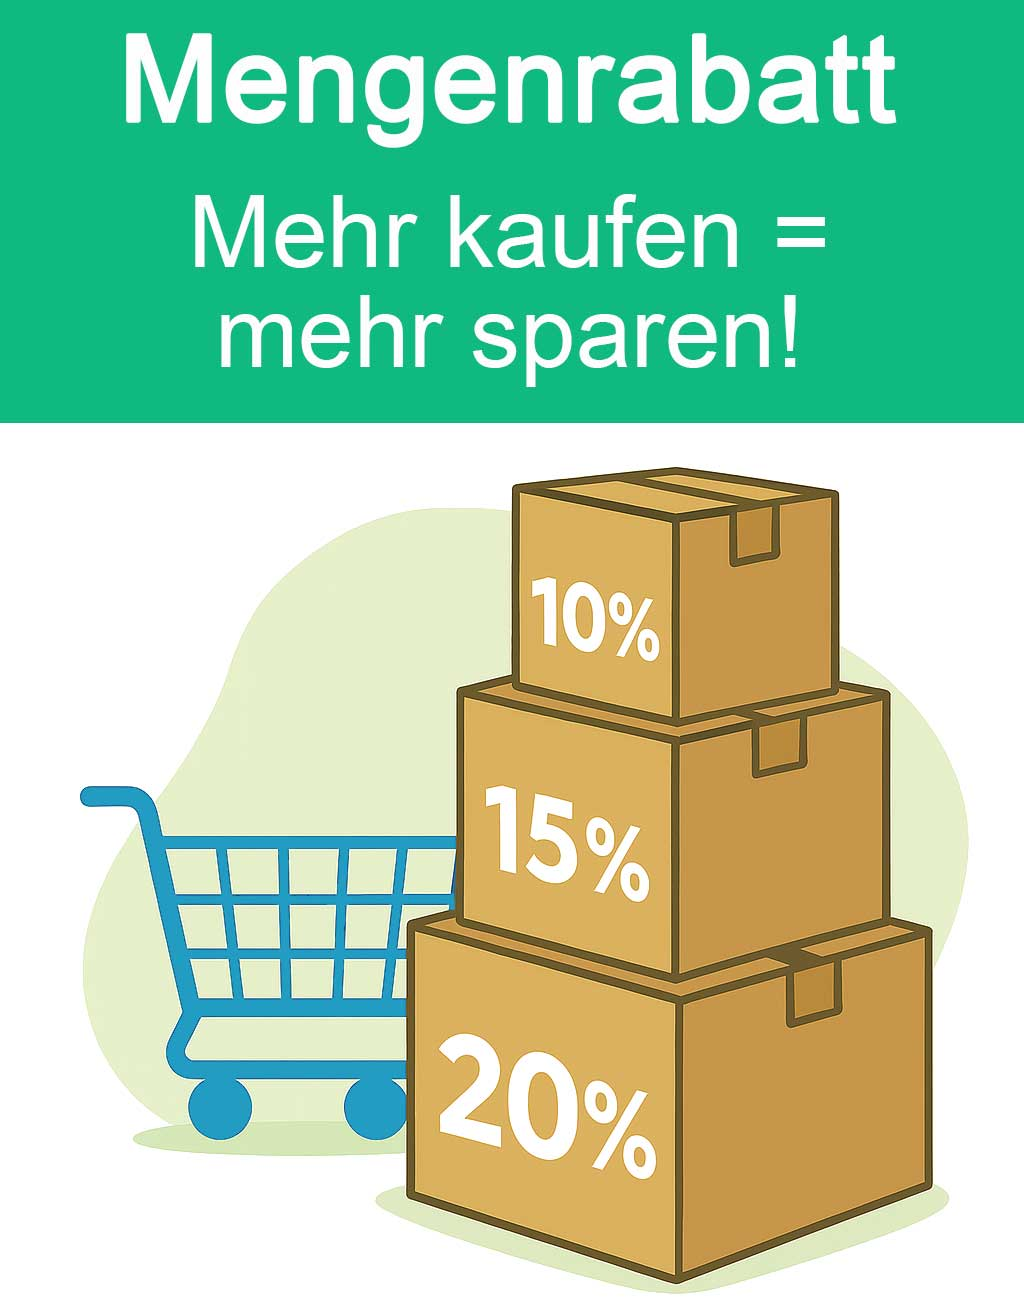
\includegraphics[width=0.5\linewidth]{BSZ_kap_14_2026/by_slide/slide_014/BSZ_kap_14_2026_slide_014_asset_01_image5.jpeg}
  \caption{Mengenrabatt -- illustrerer superior assets: bedrifter med skalafordeler kan levere fringe benefits billigere per nyttekrone enn konkurrenten. (BSZ kap.\ 14, slide 14) [SLIDE]}
\end{figure}

\subsection*{Grafisk modell -- optimal lønnsmix}

\begin{figure}[H]
  \centering
  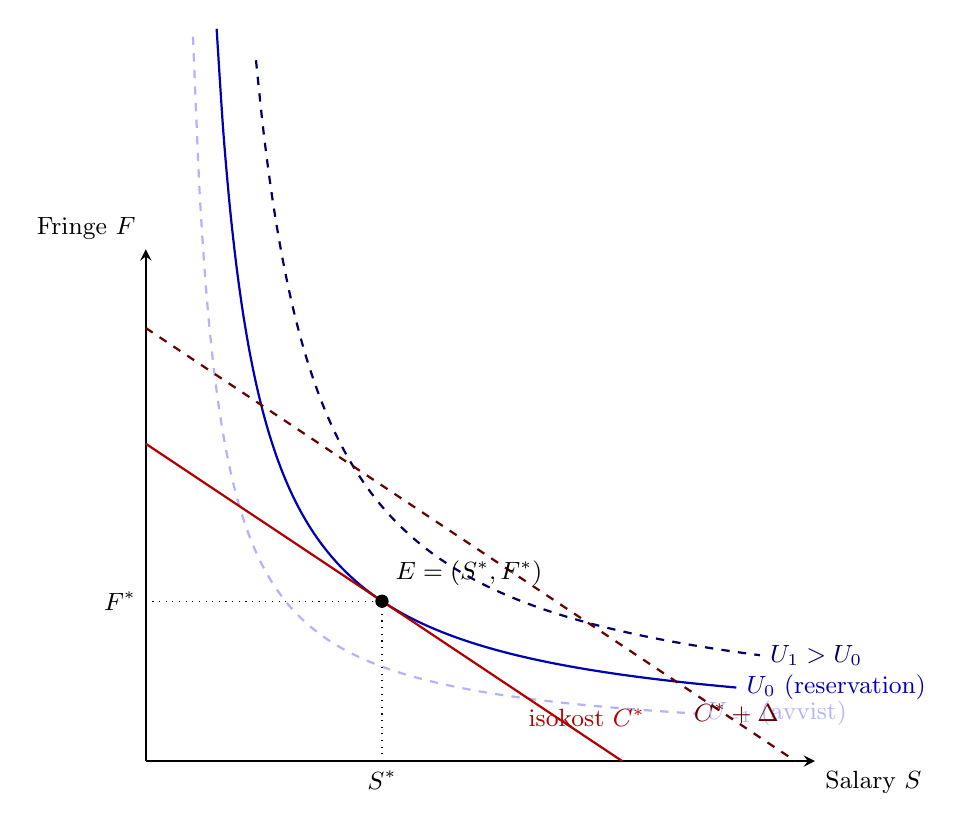
\begin{tikzpicture}[scale=1.0, >=stealth]
    \draw[->, thick] (0,0) -- (8.5,0) node[below right] {\small Salary $S$};
    \draw[->, thick] (0,0) -- (0,6.5) node[above left] {\small Fringe $F$};

    % Indifferenskurver
    \draw[blue!70!black, thick, domain=0.9:7.5, smooth, samples=80]
      plot (\x, {4.5/(\x-0.4) + 0.3}) node[right] {\small $U_0$ (reservation)};
    \draw[blue!40!black, thick, dashed, domain=1.4:7.8, smooth, samples=80]
      plot (\x, {6.8/(\x-0.6) + 0.4}) node[right] {\small $U_1 > U_0$};
    \draw[blue!30, thick, dashed, domain=0.6:7.0, smooth, samples=80]
      plot (\x, {2.7/(\x-0.3) + 0.2}) node[right] {\small $U_{-1}$ (avvist)};

    % Isokost
    \draw[red!70!black, thick] (0, 4.03) -- (6.05, 0);
    \node[red!70!black] at (5.6, 0.55) {\small isokost $C^*$};
    \draw[red!40!black, thick, dashed] (0, 5.5) -- (8.25, 0);
    \node[red!40!black] at (7.5, 0.6) {\small $C^* + \Delta$};

    % Optimum
    \filldraw[black] (3, 2.03) circle (2.2pt);
    \node[anchor=south west] at (3.05, 2.1) {\small $E = (S^*, F^*)$};
    \draw[dotted] (3, 0) -- (3, 2.03);
    \draw[dotted] (0, 2.03) -- (3, 2.03);
    \node[below] at (3, 0) {\small $S^*$};
    \node[left] at (0, 2.03) {\small $F^*$};
  \end{tikzpicture}
  \caption{Optimal mix mellom lønn $S$ og fringe $F$. Konvekse indifferenskurver $U_{-1}, U_0, U_1$ reflekterer at $S$ og $F$ er imperfekte substitutter i ansattes nytte. Isokostnadslinjer har helning $-c_S/c_F$. Optimum $E$: laveste isokost som berører $U_0$. Hvis $c_F$ synker (skatt, skala, superior asset) blir isokost flatere $\Rightarrow$ mer $F^*$, mindre $S^*$. Hvis $U_0$ stiger (stramt marked) flyttes hele kurven utover $\Rightarrow$ høyere total kostnad. [SLIDE]}
\end{figure}

\textbf{Tolkning:} I tangeringspunktet $E$ er ansattes marginale substitusjonsrate mellom lønn og fringe akkurat lik bedriftens kostnadsforhold mellom dem. Bedriften kan ikke spare penger ved å vri mixen uten å falle under $U_0$. Heterogene preferanser gir ulike indifferenskurver $\Rightarrow$ ulik optimal mix per ansatt $\Rightarrow$ rasjonale for cafeteria-style benefits. [SLIDE]

\subsection*{Real-world eksempler}

\textbf{Eks.~1 -- Equinor vs.\ Goldman Sachs (skandinavisk vs.\ angloamerikansk lønnsmix).}\quad [EKS]
For tilsvarende analytiker-/ingeniørprofiler tilbyr Equinor moderat kontantlønn, men tung fringe: omfattende pensjon via Statens pensjonskasse-aktig struktur, helseforsikring, lang ferie, langsiktig karrierevei på tvers av olje/gass/fornybar. Goldman Sachs tilbyr motsatt mix: høy grunnlønn + stor variabel bonus, lite formell fringe, kortere ansiennitetsfordeler. Forskjellen reflekterer (i) ulik $c_F$ (skandinavisk skattefavør og skala på Equinor; mindre fordel i USA), (ii) ulik $U_0$ for målgruppene (Goldman-kandidatens alternativ er hedge funds; Equinor-kandidatens er andre nordiske energiselskaper), og (iii) ulike superior assets -- Equinor har langsiktig stabilitet, Goldman har prestisje og prestasjons-signaling. Begge er optimum gitt egne $c_S, c_F, U_0$ og preferanser; ingen er ``riktig''.

\textbf{Eks.~2 -- Novo Nordisk vs.\ ung biotech-startup.}\quad [EKS]
Novo Nordisk har et superior asset i form av forskningsmiljø (eneste i verdensklasse innen diabetes), skala på fringe (helse, barnepass, kantine), og stiftelsesstabilitet -- en biokjemiker får høy ikke-monetær nytte og rimelige fringe-goder. Optimum: moderat $S^*$, høyt $F^*$, og lav total kostnad relativt til $U_0$. Ung biotech-startup (f.eks.\ Evaxion eller mindre Medicon Valley-aktør) mangler disse assetene -- må kompensere med høyere kontant grunnlønn og opsjoner, fordi $c_F$ er høy (ingen skala) og ikke-monetær superior asset er svakere. Samme markedskandidat, samme $U_0$, men ulike isokostnadslinjer $\Rightarrow$ ulike optimale mix.

\subsection*{Kobling til Mærsk Power-to-X}\quad [CASE]
PtX-divisjonen konkurrerer om scarce elektrolyse- og prosjektingeniør-talent mot Ørsted, Siemens Energy, Topsoe og Hydrogen-startups. \textbf{Reservation utility} settes i hjemmemarkedet av Ørsted (renomme i havvind, danske forhold). Mærsk PtX må overstige $U_0$, men ikke nødvendigvis ved å matche Ørsteds lønn krone for krone -- de vrir mixen mot fringe og ikke-monetære goder der Mærsks \textbf{superior assets} er rimeligere å levere enn for konkurrenten: (i) global merkevare og krysskonsern-karrierevei (shipping $\to$ logistikk $\to$ PtX $\to$ Maersk Energy), (ii) stiftelseseier som signaliserer langsiktig jobbsikkerhet, (iii) København-HQ-velferdsgoder (kantine, sentral lokasjon, familiefringe), (iv) prestisje fra A.P.\ Møller-tradisjonen. \textbf{Compensating differentials} er i tillegg relevant fordi mange PtX-anlegg vil ligge avsidesliggende (havvindkobling, areal, billig strøm) -- her må Mærsk legge på lokasjons-tillegg eller fly-in/fly-out-ordninger. Resultatet er et $(S^*, F^*)$-optimum med mer $F$ og mindre $S$ enn Ørsteds, til lavere total kostnad per ansatt -- forutsatt at superior assetene faktisk leverer reell nytte.

\subsection*{Fallgruber}
\begin{itemize}\setlength{\itemsep}{2pt}
\item Glemme at $U_0$ er en \emph{indifferenskurve}, ikke et lønnsbeløp -- multidimensjonal.
\item Forveksle compensating differentials med ren risikopremie i \thref{principal-agent}{prinsipal--agent}; det første kompenserer for jobbtrekk, det andre for risikoeksponering.
\item Påstå at fringe alltid er optimalt -- forutsetter $c_F < c_S$ (skatt, skala) og passende preferanser.
\item Tegne indifferenskurver konkave eller rette i stedet for konvekse.
\item Glemme at superior asset \emph{må} levere reell nytte for at det skal funke -- ellers er ``kultur'' bare et påskudd for å betale mindre.
\item Glemme at heterogene preferanser begrunner cafeteria-style design.
\item Behandle modellen som statisk -- $U_0$, $c_S$ og $c_F$ endrer seg med konjunktur, skatt og bedriftens livssyklus.
\item Hoppe over grafen -- spørsmålet ber eksplisitt om å \emph{vise en modell}.
\end{itemize}

\FloatBarrier
\subsection*{Håndskrivbar disposisjon (15-min forberedelse)}

\begin{figure}[H]
  \centering
  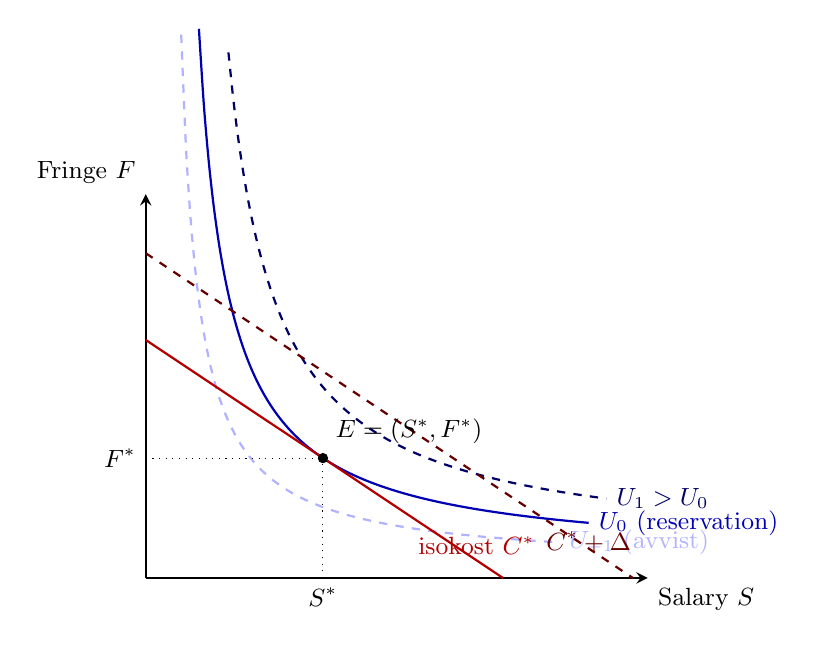
\begin{tikzpicture}[scale=0.75, >=stealth]
    \draw[->, thick] (0,0) -- (8.5,0) node[below right] {\small Salary $S$};
    \draw[->, thick] (0,0) -- (0,6.5) node[above left] {\small Fringe $F$};

    % Indifferenskurver
    \draw[blue!70!black, thick, domain=0.9:7.5, smooth, samples=80]
      plot (\x, {4.5/(\x-0.4) + 0.3}) node[right] {\small $U_0$ (reservation)};
    \draw[blue!40!black, thick, dashed, domain=1.4:7.8, smooth, samples=80]
      plot (\x, {6.8/(\x-0.6) + 0.4}) node[right] {\small $U_1 > U_0$};
    \draw[blue!30, thick, dashed, domain=0.6:7.0, smooth, samples=80]
      plot (\x, {2.7/(\x-0.3) + 0.2}) node[right] {\small $U_{-1}$ (avvist)};

    % Isokost
    \draw[red!70!black, thick] (0, 4.03) -- (6.05, 0);
    \node[red!70!black] at (5.6, 0.55) {\small isokost $C^*$};
    \draw[red!40!black, thick, dashed] (0, 5.5) -- (8.25, 0);
    \node[red!40!black] at (7.5, 0.6) {\small $C^* + \Delta$};

    % Optimum
    \filldraw[black] (3, 2.03) circle (2.2pt);
    \node[anchor=south west] at (3.05, 2.1) {\small $E = (S^*, F^*)$};
    \draw[dotted] (3, 0) -- (3, 2.03);
    \draw[dotted] (0, 2.03) -- (3, 2.03);
    \node[below] at (3, 0) {\small $S^*$};
    \node[left] at (0, 2.03) {\small $F^*$};
  \end{tikzpicture}
  \caption{Salary--fringe-modellen (referansefigur for disposisjonen): konvekse indifferenskurver, rett isokost, optimum $E$ i tangeringspunktet. [SLIDE]}
\end{figure}

\begin{itemize}\setlength{\itemsep}{2pt}
\item \textbf{Tese:} Kompensasjon = sett sammen pakke ($S, F$, ikke-monetær) som passerer $U_0$ til lavest kostnad. Optimum = tangering indifferenskurve $\leftrightarrow$ isokost.
\item \textbf{Mål med kompensasjon:} tiltrekke, retentere, motivere.
\item \textbf{\thref{reservation-utility}{Reservation utility} $U_0$:} gulv, neste-beste alternativ, multidimensjonal, participation constraint.
\item \textbf{\thref{compensating-differentials}{Compensating differentials}:} tillegg for uattraktive trekk (risiko, skift, isolasjon). Adam Smith $\to$ Rosen 1974.
\item \textbf{\thref{superior-assets}{Superior assets}:} firmaspesifikke fordeler som senker $c_F$ -- skatt, skala, brand, kultur, karrierevei.
\item \textbf{\thref{salary-fringe-benefits-mix}{Salary--fringe-modellen}:} $\min c_S S + c_F F$ s.t. $U(S,F) \geq U_0 \Rightarrow \mathrm{MRS} = c_S/c_F$.
\item \textbf{Graf:} indifferens $U_0$ konveks, isokost rett, optimum $E$ tangering, dotted projeksjoner til $S^*, F^*$.
\item \textbf{Heterogene preferanser:} ulike kurver $\Rightarrow$ cafeteria-style benefits.
\item \textbf{Eks.\ 1:} Equinor (mye fringe) vs.\ Goldman (mye $S$). Ulike $c_F$, $U_0$, superior assets.
\item \textbf{Eks.\ 2:} Novo Nordisk (forskningsmiljø + skala) vs.\ liten biotech (må overby på $S$).
\item \textbf{Case Mærsk PtX:} $U_0$ satt av Ørsted; superior assets (brand, krysskonsern, stiftelse, HQ) lar dem vri mot $F$; compensating differential for remote anlegg.
\item \textbf{Søyle:} \SThree\ primært; \SOne\ via karriere-/rolleallokering.
\end{itemize}

% !TEX root = ../main.tex
\section{Q09: Optimale valg av medarbeideres innsats -- agentens og prinsipalens side}\label{q:09}

\begin{quote}
\emph{Vis og forklar modellerne der anviser optimale valg af medarbejderes indsats -- set både fra medarbejderens (agentens) side og virksomhedens (principalens) side. Diskuter forhold som: a) risiko, b) præstationsuafhængig løn, c) incitamentskoefficienter.}
\end{quote}

\subsection*{Svar (kort)}
Spørsmålet besvares med den lineære principal-agent-modellen: output $Q=\alpha e+\mu$ (innsats $e$ ganger produktivitet $\alpha$, pluss støy $\mu$) og lønn $W=W_0+\beta Q$ (fastlønn $W_0$ pluss en andel $\beta$ av resultatet). \emph{Agenten} velger innsats $e^{*}$ slik at marginalt insentiv $\beta\alpha$ er lik marginal innsatskostnad $c'(e)$ -- altså arbeider hun helt til ekstra kroner fra bonus akkurat dekker ekstra slit. \emph{Prinsipalen} velger insentivkoeffisienten $\beta^{*}=1/(1+r\sigma^{2}c''/\alpha^{2})$. Intuitivt: jo høyere risikoaversjon ($r$) eller støy ($\sigma^{2}$), jo lavere bør $\beta$ settes -- fordi det blir dyrt å lesse risiko over på en risikoavers agent. (a) Risiko ($r$, $\sigma^{2}$) trekker $\beta^{*}$ ned; (b) den prestasjonsuavhengige $W_0$ vrir \emph{ikke} innsats, men dekker deltakelseskravet (IR -- Individual Rationality, dvs.\ at jobben må være verdt det) pluss risikopremie; (c) $\beta$ er det eneste insentivverktøyet som faktisk vrir innsats. [SLIDE]

\subsection*{De to modellene (oversikt)}

\begin{center}
\renewcommand{\arraystretch}{1.15}
\begin{tabular}{@{}p{2.8cm}p{3.6cm}p{4.4cm}p{4.6cm}@{}}
\toprule
\textbf{Side} & \textbf{Beslutningsvariabel} & \textbf{Mål} & \textbf{Optimum (FOC)} \\
\midrule
Agent & Innsats $e$ & Max $\mathbb{E}[W]-\tfrac{r}{2}\mathrm{Var}[W]-c(e)$ & $\beta\alpha=c'(e^{*})$ \\
Prinsipal & Kontrakt $(W_0,\beta)$ & Max $\mathbb{E}[Q-W]$ s.t.\ IR + IC & $\beta^{*}=\dfrac{1}{1+r\sigma^{2}c''/\alpha^{2}}$ \\
\bottomrule
\end{tabular}
\end{center}

\subsection*{Relevante teorier (kort)}

\paragraph{\thref{optimal-effort-model}{Optimal effort-modell (begge sider)}\quad\STwo/\SThree}
Modellen i BSZ kap.\ 15: output $Q=\alpha e+\mu$ (det agenten produserer), kontrakt $W=W_0+\beta Q$, og en konveks innsatskostnad $c(e)$ -- ``konveks'' fordi siste innsats-time gjør mer vondt enn første. Agentens FOC -- førsteordensbetingelsen, dvs.\ regelen for hva som maksimerer agentens nytte -- er $\beta\alpha=c'(e^{*})$. Sagt enkelt: agenten jobber til marginal bonus akkurat dekker marginal slit. Innsats er derfor strengt stigende i $\beta$ (mer bonus $\Rightarrow$ mer innsats) og uavhengig av $W_0$ (fastlønn endrer ikke marginalvurderingen). Prinsipalen tar agentens beste respons med i regnestykket og velger $\beta^{*}$ der marginal insentivgevinst er lik marginal risikopremie. Modellen leverer dermed begge optimumsbetingelsene i samme ramme og forklarer hvorfor \emph{second-best} -- nest-beste utfall, dvs.\ det beste man får når innsats ikke kan observeres -- har $\beta<1$. [SLIDE]

\paragraph{\thref{fixed-vs-variable-pay}{Prestasjonsuavhengig lønn ($W_0$) vs.\ variabel ($\beta Q$)}\quad\SThree}
$W_0$ er en ren \emph{nivå}-variabel: den løfter hele lønnsnivået og oppfyller deltakelsesskranken (IR -- jobben må gi minst like mye nytte som beste alternativ), og kompenserer agenten for risikopremien $\tfrac{r}{2}\beta^{2}\sigma^{2}$. Den vrir \emph{ikke} marginal innsats, fordi $W_0$ utbetales uansett hva agenten gjør. $\beta Q$ er derimot en ren \emph{marginal}-variabel: hver ekstra produserte enhet gir mer bonus, så innsats vris -- men risiko fra støyen $\mu$ overføres til agenten. Bare $W_0$ (uten bonus) gir \emph{shirking} (lav innsats / lureri); bare $\beta Q$ (uten fastlønn) gir ineffektiv risikodeling. Hybridkontrakter er derfor normen: $W_0$ håndterer deltakelse og risiko, $\beta Q$ håndterer innsats. [SLIDE]

\paragraph{\thref{incentive-coefficient}{Insentivkoeffisient $\beta=\partial W/\partial Q$}\quad\SThree}
$\beta$ måler ``pay-performance sensitivity'' (lønnsfølsomhet for resultat) -- hvor mange ekstra kroner lønn én ekstra krone resultat gir. Determinanter: $\beta^{*}$ stiger med produktivitet $\alpha$ (sterkere kobling mellom innsats og output $\Rightarrow$ mer å hente på å gi bonus); $\beta^{*}$ faller med risikoaversjon $r$, støy $\sigma^{2}$ og kostnadens konveksitet $c''$ (jo brattere kostnadskurven blir, jo mindre ekstra innsats får man uansett). Empirisk varierer $\beta$ fra omtrent $0$ (tariffstillinger som sykepleier) til omtrent $1$ (\emph{franchising} -- der franchisetaker eier hele residualen, og \emph{residual claimancy} betyr at agenten beholder alt overskudd). Holmström--Milgrom (1991): hvis agenten har flere oppgaver der bare én er målbar (\emph{multitasking}), må $\beta$ senkes -- ellers vil agenten dumpe de umålbare oppgavene og bare jobbe med det som teller på bonusen. [SLIDE]

\paragraph{\thref{risk-sharing}{Risikodeling}\quad\SThree}
Risikoavers agent + diversifisert risikonøytral prinsipal (en eier som spør lite om risiko, fordi formuen er spredt) $\Rightarrow$ \emph{Pareto-optimal} (ingen kan bli bedre stilt uten at noen blir verre stilt) risikodeling tilsier first-best, dvs.\ ren fastlønn til agenten -- eieren bærer all risikoen. Men da forsvinner insentivet til å jobbe. Second-best krever at agenten bærer \emph{noe} risiko gjennom $\beta>0$, og prinsipalen må kompensere med en risikopremie. Risikopremien $\tfrac{r}{2}\beta^{2}\sigma^{2}$ -- som intuitivt sier at risikokostnaden vokser med kvadratet av $\beta$ og lineært med agentens risikoaversjon og støyen -- er kjernen i \thref{agency-costs}{agency costs} (kostnaden ved at agenten ikke kan bli direkte styrt) i denne modellen. Når $\sigma^{2}$ er stor, brukes \thref{informativeness-principle}{informativeness-mekanismer} -- altså tilleggssignaler som filtrerer bort eksogen støy -- som relative måltall, peer-grupper og indekserte opsjoner. [SLIDE]

\subsection*{Illustrasjoner fra forelesning}

\begin{figure}[H]
  \centering
  
\includegraphics[width=0.4\linewidth]{BSZ_kap_15_2026/by_slide/slide_002/BSZ_kap_15_2026_slide_002_asset_01_image1.png}
  \caption{Insentivkompensasjon: agenten responderer på $\beta$ -- høyere pay-performance sensitivity gir sterkere innsats, men krever risikopremie. (BSZ kap.\ 15, slide 2) [SLIDE]}
\end{figure}

\subsection*{Grafisk modell -- to bilder (agent + prinsipal)}

\begin{figure}[H]
\centering

\includegraphics[width=0.55\linewidth]{BSZ_kap_15_2026/by_slide/slide_014/BSZ_kap_15_2026_slide_014_asset_01_image3.png}
\caption{Pensumets versjon av principal-agent-modellen: $Q=\alpha e+\mu$ og $W=W_0+\beta Q$. [SLIDE -- BSZ kap.\ 15, slide 14]}
\end{figure}

Agentens side kan tegnes på to måter, som henger sammen som ``totalbildet'' og ``marginalbildet'' av samme optimum: (1) \emph{totalkurver} -- kompensasjon $W=W_0+\beta\alpha e$ som rett linje og kostnad $c(e)=e^{2}$ som konveks kurve, hvor $e^{*}$ er der tangenten til kostnadskurven er parallell med kompensasjonslinjen; (2) \emph{deriverte kurver} -- $MB=\beta\alpha$ horisontal og $MC=c'(e)=2e$ stigende, hvor $e^{*}$ er rett krysningspunkt. Det er samme FOC ($\beta\alpha=c'(e^{*})$), bare lest ut av to forskjellige grafer.

\begin{figure}[H]
\centering
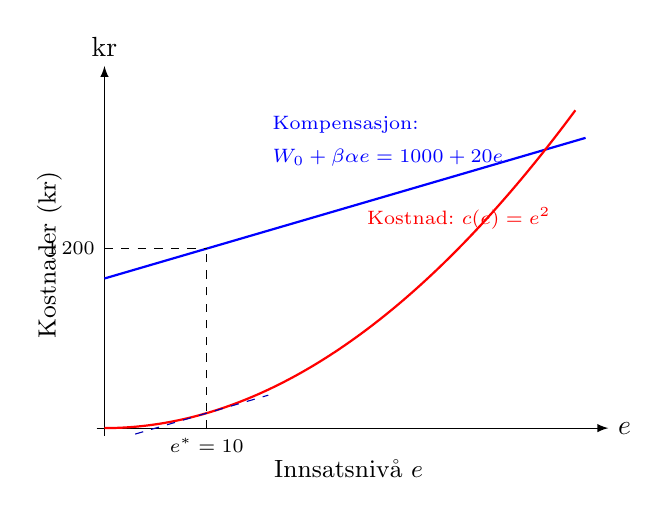
\begin{tikzpicture}[>=latex]
  % Skalafaktorer: 1 effort-enhet = 0.13 cm, 1 kr = 0.0019 cm
  % Akser (i cm)
  \draw[->] (-0.1,0) -- (6.4,0) node[right] {$e$};
  \draw[->] (0,-0.1) -- (0,4.6) node[above] {kr};
  \node[below=8pt] at (3.1,0) {\small Innsatsnivå $e$};
  \node[rotate=90] at (-0.7,2.2) {\small Kostnader (kr)};
  % Kompensasjonslinje W = 1000 + 20e (cm: x=e*0.13, y=W*0.0019)
  \draw[thick,blue] (0,1.9) -- (6.11,3.686);
  \node[blue,above,align=left] at (3.6,3.2) {\scriptsize Kompensasjon:\\ \scriptsize $W_0+\beta\alpha e=1000+20e$};
  % Kostnadskurve c(e) = e^2
  \draw[thick,red,domain=0:46,samples=80,smooth]
    plot ({\x*0.13},{\x*\x*0.0019});
  \node[red,above] at (4.5,2.4) {\scriptsize Kostnad: $c(e)=e^{2}$};
  % Tangent ved e*=10 (stigning 20): y = 20e - 100
  \draw[dashed,blue!70!black] (0.39,-0.076) -- (2.08,0.418);
  % Hjelpe-streker for e*=10 og W=1200
  \draw[dashed] (1.3,0) -- (1.3,2.28);
  \draw[dashed] (0,2.28) -- (1.3,2.28);
  \node[left] at (0,2.28) {\scriptsize $1\,200$};
  \node[below] at (1.3,0) {\scriptsize $e^{*}=10$};
\end{tikzpicture}
\caption{\textbf{Agentens side -- totalmodellen (ikke-derivert).} Kompensasjonslinjen $W=W_0+\beta\alpha e$ (her $W_0=1000$, $\beta\alpha=20$) og den konvekse kostnadskurven $c(e)=e^{2}$. Agenten velger $e^{*}=10$ der tangenten til kostnadskurven er parallell med kompensasjonslinjen -- altså $c'(e^{*})=2e^{*}=20=\beta\alpha$. Total kompensasjon ved $e^{*}$: $W=1\,200$. Krever \texttt{\textbackslash usepackage\{tikz\}} i preamble.}
\end{figure}

\begin{figure}[H]
\centering
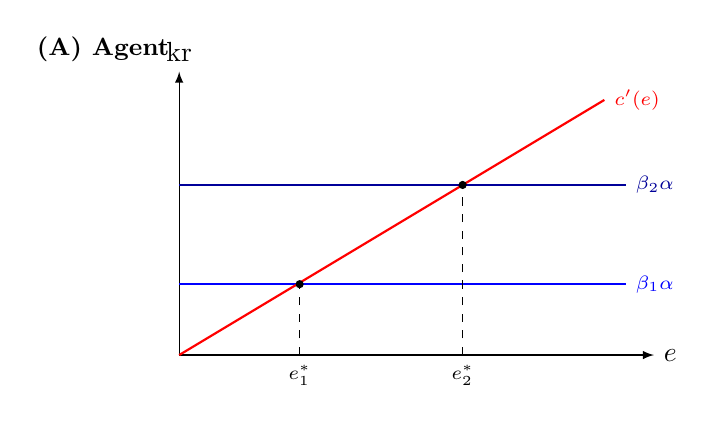
\begin{tikzpicture}[>=latex,scale=0.9]
  % Akser
  \draw[->] (0,0) -- (6.7,0) node[right] {$e$};
  \draw[->] (0,0) -- (0,4.0) node[above] {kr};
  \node[above left] at (0,4.0) {\small \textbf{(A) Agent}};
  % MB-linjer
  \draw[thick,blue] (0,1.0) -- (6.3,1.0) node[right] {\scriptsize $\beta_1\alpha$};
  \draw[thick,blue!60!black] (0,2.4) -- (6.3,2.4) node[right] {\scriptsize $\beta_2\alpha$};
  % MC
  \draw[thick,red] (0,0) -- (6.0,3.6) node[right] {\scriptsize $c'(e)$};
  % Optima
  \draw[dashed] (1.7,0) -- (1.7,1.0); \filldraw (1.7,1.0) circle (1.4pt);
  \node[below] at (1.7,0) {\scriptsize $e_1^{*}$};
  \draw[dashed] (4.0,0) -- (4.0,2.4); \filldraw (4.0,2.4) circle (1.4pt);
  \node[below] at (4.0,0) {\scriptsize $e_2^{*}$};
\end{tikzpicture}\quad
\begin{tikzpicture}[>=latex,scale=0.9]
  % Akser
  \draw[->] (0,0) -- (6.7,0) node[right] {$\beta$};
  \draw[->] (0,0) -- (0,4.0) node[above] {kr};
  \node[above left] at (0,4.0) {\small \textbf{(B) Prinsipal}};
  \draw (5.2,0) node[below] {\scriptsize $1$};
  \draw[dashed] (5.2,0) -- (5.2,3.2);
  % MB(β) konkav
  \draw[thick,blue,domain=0:5.2,samples=60]
    plot (\x,{3.0*(1-exp(-0.7*\x))}) node[right] {\scriptsize $MB(\beta)$};
  % MC(β) konveks
  \draw[thick,red,domain=0:5.2,samples=60]
    plot (\x,{0.35*\x*\x}) node[right] {\scriptsize $MC(\beta)$};
  % Krysning -- MB(2.7)=2.55, MC(2.7)=0.35*7.29=2.55
  \filldraw (2.7,2.55) circle (1.4pt);
  \draw[dashed] (2.7,0) -- (2.7,2.55);
  \node[below] at (2.7,0) {\scriptsize $\beta^{*}$};
\end{tikzpicture}
\caption{\textbf{(A) Agentens side:} $e^{*}$ der $\beta\alpha=c'(e)$; en høyere $\beta$ skifter $MB$ opp og $e^{*}$ til høyre. \textbf{(B) Prinsipalens side:} $\beta^{*}$ der marginal insentivgevinst lik marginal risikopremie $\tfrac{r}{2}\beta^{2}\sigma^{2}$; $\beta^{*}<1$ i second-best. Krever \texttt{\textbackslash usepackage\{tikz\}} i preamble.}
\end{figure}

\textbf{Hvordan de to grafene henger sammen.} Grafene leses sekvensielt: prinsipalen velger $\beta^{*}$ i (B) ved å forutse at agenten vil reagere i (A). Hver verdi av $\beta$ i (B) bestemmer hvor høyt $MB$-linja ligger i (A), og dermed agentens $e^{*}$. Når prinsipalen øker $\beta$, øker insentivgevinsten (mer $e$, mer $Q$) -- men også risikopremien som prinsipalen må betale via $W_0$ for å holde IR. Optimum er der \emph{disse to skråningene treffer hverandre}: avtagende marginalgevinst (konkav $MB$) møter stigende marginal risikokostnad (konveks $MC$). Det er nettopp denne trade-offen som gir Holmström-Milgrom-formelen for $\beta^{*}$ og som forklarer hvorfor $\beta^{*}<1$ alltid med risikoavers agent.

\subsection*{Real-world eksempler}

\textbf{Eks.~1 -- Investment banking-trader vs.\ Statoil/Equinor-toppleder.}\quad [EKS]
Tradere i internasjonale banker har lav $W_0$ (relativt) og høy $\beta$ -- prestasjonen er målbar (P\&L), agenten er typisk lite risikoavers, og produktiviteten ($\alpha$) er stor. I motsetning har Equinor-konsernsjefen en betydelig grunnlønn og en moderat $\beta$ levert via aksjebasert LTI med peer-justering -- fordi oljepris ($\mu$) gir stor støy ($\sigma^{2}$) som må filtreres for at risikopremien ikke skal eksplodere. Samme modell, ulik parametertilstand: traderen sitter ved $\beta\to 1$-enden, Equinor-CEO ved moderat $\beta$.

\textbf{Eks.~2 -- Norsk offentlig sektor vs.\ Aker Solutions provisjons-selger.}\quad [EKS]
Sykepleier i kommunal helse har $\beta\approx 0$, ren tarifflønn: output er svært vanskelig å måle, agenten er risikoavers, og fordelingshensyn favoriserer fastlønn. Aker Solutions selger av offshore-utstyr har $\beta\approx 0{,}3$--$0{,}5$ på kvartals-salgsmål, lavere $W_0$, og bonusen er ``claw-back''-pliktig hvis kunden trekker seg. Sammenligning: identisk modell, men ulike $(\alpha,r,\sigma^{2})$ tvinger fram diametralt motsatte kontrakter. Dette viser at modellen er en \emph{designkalkulator}, ikke en universaloppskrift.

\subsection*{Kobling til Mærsk Power-to-X}
PtX-divisjonens utfall avhenger sterkt av eksogen elektrisitetspris og hydrogen-etterspørsel -- et stort $\sigma^{2}$. Modellen tilsier derfor \emph{lav $\beta$} på topplinjeresultat (EBITDA, NPV) for divisjonsledelsen, fordi å overføre denne risikoen til risikoaverse ledere ville krevd en kostbar risikopremie. Likevel: noe $\beta$ kan kobles til \emph{kontrollerbare milestones} -- anlegg ferdigstilt i tide, OPEX innenfor budsjett, kontrakter signert med PtX-avtakere. Dette er \thref{informativeness-principle}{informativeness-prinsippet} i praksis: bruk de måltall som faktisk signalerer innsats, ikke de som domineres av eksogen støy. Hybridkontrakten (høy $W_0$, lav $\beta$ på finansresultater, moderat $\beta$ på milestones) er Mærsk-konsistent med en risikoavers ledelse i et høy-$\sigma^{2}$-prosjekt. [CASE]

\subsection*{Fallgruber}
\begin{itemize}\setlength{\itemsep}{2pt}
\item Glemme at $W_0$ \emph{ikke} vrir innsats -- klassisk forveksling av nivå og marginal.
\item Anta at høyere $\beta$ alltid er bedre -- ignorerer risikopremien og multitasking.
\item Bare beskrive agentens side uten å vise prinsipalens optimeringsproblem (eller omvendt).
\item Glemme støyen $\mu$ og dens rolle for $\beta^{*}$ -- spørsmålet nevner risiko eksplisitt.
\item Sette $\beta^{*}=1$ uten å forklare at det krever risikonøytral agent eller observerbar innsats.
\item Forveksle insentivproblemet (\thref{moral-hazard}{moral hazard}) med risikodelingsproblemet -- de er separate, men koblet via $\beta$.
\item Tegne MC- og MB-kurvene feil vei (MC stigende, MB i $\beta$ konkav) -- få graf-detaljer galt skader troverdighet.
\end{itemize}

\FloatBarrier
\subsection*{Håndskrivbar disposisjon (15-min forberedelse)}
\begin{itemize}\setlength{\itemsep}{2pt}
\item \textbf{Tese:} To FOC -- agentens for $e^{*}$, prinsipalens for $\beta^{*}$ -- innenfor samme lineære principal-agent-modell.
\item \textbf{Setup:} $Q=\alpha e+\mu$, $W=W_0+\beta Q$, agent CARA + $c(e)$, prinsipal diversifisert.
\item \textbf{Agentside (Modell A):} Max $\mathbb{E}[W]-\tfrac{r}{2}\mathrm{Var}[W]-c(e)\Rightarrow \beta\alpha=c'(e^{*})$. Ian/AssemCo: $e^{*}=50\beta$. \emph{$W_0$ vrir ikke innsats.}
\item \textbf{Prinsipalside (Modell B):} Max $\alpha e^{*}-c(e^{*})-\tfrac{r}{2}\beta^{2}\sigma^{2}\Rightarrow \beta^{*}=\tfrac{1}{1+r\sigma^{2}c''/\alpha^{2}}$.
\item \textbf{(a) Risiko:} $r,\sigma^{2}\uparrow\Rightarrow\beta^{*}\downarrow$. Risikopremien $\tfrac{r}{2}\beta^{2}\sigma^{2}$ er kjernen i agency cost.
\item \textbf{(b) $W_0$:} Faller ut av FOC; rolle = IR + risikopremie-kompensasjon. \emph{Vrir ikke innsats.}
\item \textbf{(c) $\beta$:} Eneste innsatsdriver. Pay-performance sensitivity. Determinanter: $\alpha\uparrow$, $r\downarrow$, $\sigma^{2}\downarrow$ $\Rightarrow$ $\beta\uparrow$.
\item \textbf{Graf A:} $MB=\beta\alpha$ horisontal, $MC=c'(e)$ stigende, kryss = $e^{*}$.
\item \textbf{Graf B:} $MB(\beta)$ konkav, $MC(\beta)=$ risikopremie konveks, kryss = $\beta^{*}<1$.
\item \textbf{Eks.\ 1:} IB-trader (høy $\beta$, lav $W_0$) vs.\ Equinor-CEO (moderat $\beta$, høy $W_0$, peer-justering).
\item \textbf{Eks.\ 2:} Norsk sykepleier (alt $W_0$) vs.\ Aker Solutions selger (provisjon med claw-back).
\item \textbf{Case:} Mærsk PtX -- stort $\sigma^{2}\Rightarrow$ lav $\beta$ på EBITDA, moderat $\beta$ på milestones (\thref{informativeness-principle}{informativeness}).
\item \textbf{Søyle:} \STwo\ + \SThree.
\end{itemize}

% !TEX root = ../main.tex
\section{Q10: Individuell prestasjonsmåling og -belønning -- formål og begreper}\label{q:10}

\begin{quote}
\emph{I forbindelse med individuel præstationsmåling og -belønning bedes der redegjort for formålene hermed. I forlængelse heraf redegøres for og diskuteres begreberne: a) ratchet-system / ratchet-effekt, b) gaming, c) absolut / relativ præstationsmåling, d) subjektiv / objektiv præstationsmåling.}
\end{quote}

\subsection*{Svar (kort)}
Individuell prestasjonsmåling tjener fire \emph{simultane} formål -- feedback, koordinasjon, belønning/sanksjon og støtte til den organisatoriske arkitekturen -- og fordi samme måltall presses inn i alle fire roller, oppstår de fire problemene spørsmålet ber om: ratchet-effekten, gaming, valg mellom absolutt og relativ måling, og valg mellom subjektiv og objektiv evaluering. Løsningen i BSZ kap.\ 16 er ikke ``bedre måling'' alene, men strukturelt smartere systemdesign: hybrider, bonusbanker, balansert målekort og Jensens lineære pay-for-performance. [SLIDE]

\subsection*{Formålene med individuell prestasjonsmåling og -belønning}

Se utdypning i \thref{performance-measurement-purposes}{formålene med prestasjonsmåling}. BSZ kap.\ 16 angir fire formål, som ofte drar i ulike retninger og er kilden til de etterfølgende delspørsmålene: [SLIDE]

\begin{enumerate}\setlength{\itemsep}{2pt}
\item \textbf{Feedback (læring).} Den ansatte må vite hvor hun står for å justere atferd. Krever rikt, kontinuerlig signal.
\item \textbf{Koordinasjon.} Felles måltall fungerer som retningsangiver på tvers av enheter -- definerer hva organisasjonen prioriterer.
\item \textbf{Belønning og sanksjon.} Måltallet er input til kompensasjon, forfremmelse og oppsigelse. Krever verifiserbarhet, kontrollerbarhet, informativeness.
\item \textbf{Arkitekturstøtte.} Måltallet binder \SOne\ beslutningsrettigheter og \SThree\ insentiver sammen -- ellers oppstår misalignment og residual loss (jf.\ \thref{agency-costs}{agency costs}).
\end{enumerate}

\textbf{Sentralt poeng:} Et måltall som er optimalt for ett formål er sjelden optimalt for de tre andre. Det er denne flerbruken som genererer ratchet, gaming og hele subjektiv/objektiv-debatten. [SLIDE]

\subsection*{Relevante begreper (kort)}

\paragraph{a) \thref{ratchet-effect}{Ratchet-system og ratchet-effekt}\quad\STwo/\SThree}
Et \emph{ratchet-system} er målsetting som bygger neste periodes mål på inneværende periodes ytelse. \emph{Ratchet-effekten} er agentens rasjonelle motrespons: hold igjen i dag for å unngå strammere mål i morgen -- ekstremvarianten er \emph{sandbagging}. Forutsetter gjentakelse, asymmetrisk informasjon og manglende commitment fra prinsipalen. Historisk dokumentert i sovjetisk planøkonomi (Berliner, Weitzman). Løsning: flerårige LTI, eksterne benchmarks (relativ måling), Jensens lineære pay-for-performance som bryter koblingen mellom budsjett og bonus. [SLIDE/BOK]

\paragraph{b) \thref{gaming-in-performance-measurement}{Gaming og horisontproblem}\quad\STwo}
\emph{Gaming} er manipulasjon av selve målet i stedet for å skape verdien målet representerer; \emph{horisontproblemet} er kortsiktig optimering som ofrer langsiktig verdi. Teoretisk rot: Goodhart's law -- ``når en måling blir et bonusmål, slutter den å være et godt mål.'' Holmström \& Milgrom (1991) viser at sterk insentivvekt på ett målbart mål vrir innsats bort fra ikke-målbare oppgaver (multitasking-problem). Løsninger: balansert målekort, bonusbanker, claw-back, subjektiv overstyring. [SLIDE]

\paragraph{c) \thref{absolute-vs-relative-performance}{Absolutt vs.\ relativ prestasjonsmåling}\quad\STwo}
Absolutt: målt mot fast standard, uavhengig av andre. Relativ: målt mot peer-gruppe (kolleger, eksterne benchmarks). Teorigrunnlag: Holmström (1979) \emph{informativeness principle} -- relativ måling filtrerer ut felles sjokk og gjør målet mer informativt om innsats, slik at insentivkoeffisient \thref{incentive-coefficient}{$\beta$} kan settes høyere uten å overlaste agenten med risiko. Pris: rat race, sabotasje, kunnskapshamstring (Microsoft stack ranking). Hybrid (absolutt budsjett + rTSR-overlegg) er praksis i de fleste børsnoterte LTI-programmer. [SLIDE/BOK]

\paragraph{d) \thref{subjective-vs-objective-performance}{Subjektiv vs.\ objektiv prestasjonsmåling}\quad\STwo}
Objektiv: forhåndsdefinerte, verifiserbare, kvantitative kriterier. Subjektiv: ex post helhetsvurdering av evaluator. Objektive mål er juridisk holdbare og enkle å kommunisere, men dekker bare målbare jobbdimensjoner og er gaming-utsatte. Subjektive evalueringer fanger samarbeid, lederskap og mentoring, men introduserer påvirkningskostnader, partiskhet og supervisor shirking. Nesten alltid hybrid: objektiv formel + subjektiv overstyring, gjerne kalibrert på tvers av evaluatorer. [SLIDE]

\subsection*{Illustrasjon}

\begin{figure}[h]
  \centering
  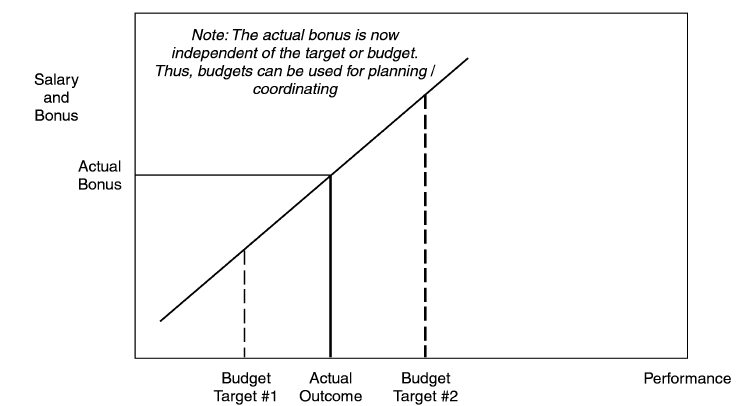
\includegraphics[width=0.6\linewidth]{BSZ_kap_16/by_slide/slide_016/BSZ_kap_16_slide_016_asset_01_image3.png}
  \caption{Tradisjonelt budget-bonus-system. Den knekkede formen (hurdle ved 80\,\%, cap ved 120\,\%) gir både gaming (rett under hurdle: skyv resultat til neste år; rett over cap: hold igjen) og ratchet-effekt (neste års mål settes fra årets resultat). (BSZ kap.\ 16, slide 16) [SLIDE]}
\end{figure}

\begin{figure}[h]
  \centering
  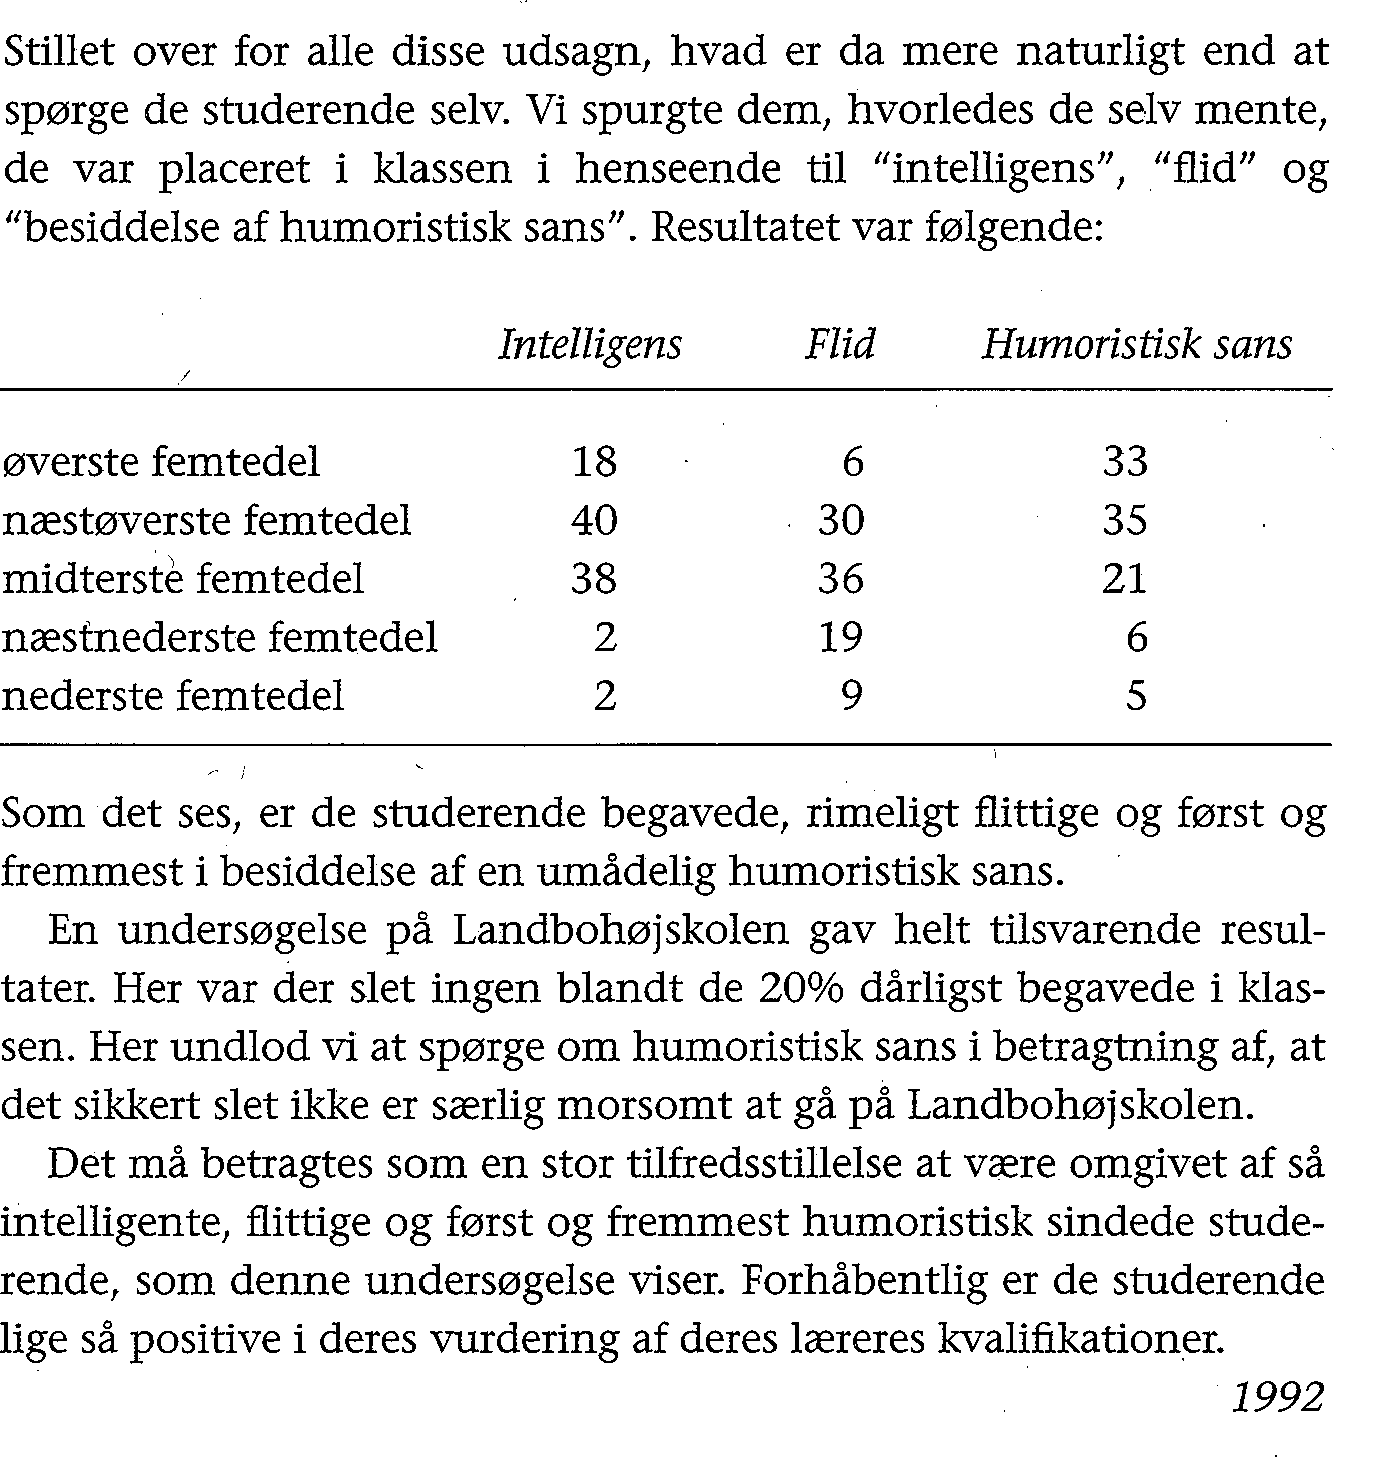
\includegraphics[width=0.6\linewidth]{BSZ_kap_16/by_slide/slide_019/BSZ_kap_16_slide_019_asset_01_image4.png}
  \caption{Jensens forslag: lineær pay-for-performance der bonus er uavhengig av budsjettet. Budsjettet brukes til planlegging og koordinasjon (formål 2), mens belønning (formål 3) er frikoblet -- da forsvinner motivasjonen for sandbagging og ratchet-tilpasning. (BSZ kap.\ 16, slide 19) [SLIDE]}
\end{figure}

\subsection*{Real-world eksempler}

\textbf{Eks.~1 -- Wells Fargo (US, 2016).}\quad [EKS]
Wells Fargo hadde aggressive cross-sell-kvoter for filialer: bonus knyttet objektivt og absolutt til antall produkter solgt per kunde. Resultatet var 3{,}5 mill.\ falske kundekontoer åpnet uten kundenes viten -- klassisk \emph{gaming} av et énmålssystem. Skandalen utløste \$185 mill.\ bot og styrtende aksjekurs. Etter skandalen omla Wells Fargo til et mer balansert system med subjektiv kvalitetsvurdering, kundetilfredshetsmål og lavere insentivvekt på ren volumvekst. Eksempelet illustrerer hvordan \emph{ren objektiv, absolutt} måling kombinert med høy $\beta$ er en gaming-katastrofe ventende.

\textbf{Eks.~2 -- Microsoft (skift 2013, sammenligning).}\quad [EKS]
Microsoft brukte fra ca.\ 2000 til 2013 ``stack ranking'': en tvungen \emph{relativ} rangering der ledere måtte plassere ansatte i forhåndsdefinerte distribusjoner og bunn-10\,\% ble vurdert ut. Systemet skapte sabotasje (ingen ville dele kunnskap med en konkurrent), kunnskapshamstring og ``hold dårlige folk i teamet for å se bedre ut selv''-strategier. I 2013 avskaffet Steve Ballmer/Satya Nadella stack ranking og innførte ``Connect''-samtaler -- en mer \emph{subjektiv, mindre relativ} evaluering med fokus på vekst og samarbeid. Sammenligningen med Wells Fargo viser at \emph{begge ytterpunktene} kan feile: Wells Fargo feilte med for objektivt og absolutt; Microsoft feilte med for relativt. Begge endte i hybrid.

\subsection*{Kobling til Mærsk Power-to-X}
PtX-prosjektledelse illustrerer flere av problemene konkret: [CASE]
\begin{itemize}\setlength{\itemsep}{2pt}
\item \textbf{Ratchet-fare} hvis ``anlegg-ferdigstilt-per-år'' brukes som mål uten korreksjon for prosjektmodning -- lederen lærer å holde igjen for å unngå strammere mål neste år.
\item \textbf{Gaming/horisontproblem} hvis kortsiktig OPEX brukes som måltall -- vedlikehold på elektrolysører utsettes for å pynte på årets tall.
\item \textbf{Løsning -- hybrid:} Objektive milestones (FID, kontrakter signert, IRR-måltall) for verifiserbarhet og juridisk holdbarhet, kombinert med \emph{subjektiv} ratifisering av kvalitet og partnervalg via \thref{decision-management-control}{Decision Control}-instans i konsernledelsen.
\item \textbf{Relativ benchmarking} mot andre PtX-prosjekter (Ørsted, Air Liquide) filtrerer ut bransje-sjokk (elpris, hydrogen-etterspørsel) og isolerer lederens reelle bidrag (jf.\ \thref{controllability-principle}{controllability}).
\end{itemize}

\subsection*{Fallgruber}
\begin{itemize}\setlength{\itemsep}{2pt}
\item Glemme \emph{formålene} -- spørsmålet ber eksplisitt om dem først. Sensorer venter alle fire (feedback / koordinasjon / belønning / arkitekturstøtte).
\item Behandle de fire begrepene som uavhengige. De er \emph{konsekvenser} av at samme måltall presses i flere formål -- vis sammenhengen.
\item Forveksle ratchet (dynamisk problem på tvers av perioder) med gaming (statisk manipulasjon innen perioden). Sandbagging er en bro: spesifik form for gaming \emph{motivert} av ratchet.
\item Beskrive relativ måling kun positivt -- nevn sabotasje, rat race, peer-pool manipulasjon.
\item Påstå at subjektiv = irrasjonell. Subjektiv evaluering er ofte mer informativ enn dårlige objektive måltall.
\item Mangle hybridløsningen. ``Verken eller, men begge med rett vekting'' er ofte BSZ-svaret.
\item Glemme Jensen-kritikken og lineær pay-for-performance som strukturell løsning på ratchet-problemet.
\item Glemme balansert målekort som svar på multitasking/gaming.
\end{itemize}

\subsection*{Håndskrivbar disposisjon (15-min forberedelse)}
\begin{itemize}\setlength{\itemsep}{2pt}
\item \textbf{Tese:} Måling tjener \emph{fire} formål samtidig -- konfliktene mellom dem genererer alle problemene i a)--d). Løsning: smartere systemdesign, ikke bare ``bedre måling''.
\item \textbf{Fire formål} (\thref{performance-measurement-purposes}{purposes}): (i) Feedback, (ii) Koordinasjon, (iii) Belønning/sanksjon, (iv) Arkitekturstøtte. Trade-offs mellom dem $\Rightarrow$ resten av spørsmålet.
\item \textbf{a) \thref{ratchet-effect}{Ratchet}:} Mål fra historie $\Rightarrow$ sandbagging. Sovjet-eksempel. Løsning: flerårig LTI, ekstern benchmark, lineær pay (Jensen).
\item \textbf{b) \thref{gaming-in-performance-measurement}{Gaming + horisont}:} Goodhart, Holmström \& Milgrom multitasking. Løsning: BSC, bonusbank, claw-back, subj.\ overstyring.
\item \textbf{c) \thref{absolute-vs-relative-performance}{Absolutt vs.\ relativ}:} Holmström '79 informativeness $\Rightarrow$ relativ filtrerer felles støy, lavere risikopremie, men sabotasje. Hybrid (rTSR).
\item \textbf{d) \thref{subjective-vs-objective-performance}{Subj.\ vs.\ obj.}:} Obj.\ verifiserbar men gaming-utsatt; subj.\ fanger multidim.\ men gir påvirkningskost + bias. Hybrid.
\item \textbf{Illustrasjon:} BSZ kap.\ 16 slide 16 (knekket budget-bonus) vs.\ slide 19 (Jensens lineære).
\item \textbf{Eks.\ 1 -- Wells Fargo 2016:} objektiv + absolutt + høy $\beta$ $\Rightarrow$ 3,5 mill.\ falske kontoer.
\item \textbf{Eks.\ 2 -- Microsoft pre/post-2013:} stack ranking (relativ + objektiv) $\Rightarrow$ sabotasje; ``Connect'' (mer subj.\ + absolutt).
\item \textbf{Case:} Mærsk PtX -- milestone-mål (obj.) + subj.\ kvalitetsratifisering + relativ benchmark mot Ørsted/Air Liquide.
\item \textbf{Søyle:} \STwo\ primært; kobler til \SOne\ (controllability) og \SThree\ ($\beta$-design).
\end{itemize}

% !TEX root = ../main.tex
\section{Q11: Boundaries of the Firm -- vertikal integrasjon, outsourcing og market power}\label{q:11}

\begin{quote}
\emph{Med udgangspunkt i termerne Boundaries of the Firm, regnskabsmæssig kontra økonomisk profit, ejerskab af produktionsfaktorer bedes begreberne vertikal integration og outsourcing præsenteret og diskuteret med hensyn til fordele og ulemper. Redegør i forlængelse heraf for modellen omhandlende vertical integration som instrument til at opnå market power.}
\end{quote}

\subsection*{Svar (kort)}
Firmaets grenser (\emph{Boundaries of the Firm}) bestemmes av avveiningen mellom transaksjonskostnader i markedet og byråkratikostnader internt (Coase 1937, Williamson 1985). Vertikal integrasjon lønner seg når spesifikke aktiva, usikkerhet og hold-up gjør markedskontrakter dyrere enn intern styring -- men den bringer egne \thref{agency-costs}{agency costs}. Sondringen mellom regnskapsmessig og økonomisk profitt avgjør om en aktivitet reelt skaper verdi innenfor firmaets grenser. Modellen for market power viser at vertikal integrasjon kan brukes strategisk til å stenge ute konkurrenter ved å kontrollere et kritisk input (foreclosure). [SLIDE]

\subsection*{Relevante teorier (kort)}

\paragraph{\thref{boundaries-of-the-firm}{Boundaries of the Firm}\quad\SOne}
Coase: firmaet erstatter markedstransaksjoner med hierarki når transaksjonskostnader er høye. Williamson: make-or-buy avhenger av asset specificity, usikkerhet og frekvens. Eierskap av produktionsfaktorer gir \emph{residuelle beslutningsrettigheter} i situasjoner kontrakten ikke dekker (Grossman--Hart--Moore). Firmaets grense trekkes der marginal intern organiseringskostnad = marginal transaksjonskostnad. [SLIDE]

\paragraph{\thref{accounting-vs-economic-profit}{Regnskabsmæssig vs.\ økonomisk profit}\quad\STwo}
Regnskapsprofitt = inntekter $-$ eksplisitte kostnader. Økonomisk profitt = inntekter $-$ alle kostnader inkl.\ \emph{opportunity cost}. En internt utført aktivitet kan vise positiv regnskapsprofitt men negativ økonomisk profitt -- da bør den outsources. BSZ Table 8.1 (BP gasoline) illustrerer: regnskapsprofitt \$1{,}2M vs.\ økonomisk profitt $-$\$400k. Kobling til \thref{responsibility-centers}{investment centers} og EVA. [SLIDE]

\paragraph{\thref{vertical-integration-outsourcing}{Vertikal integrasjon og outsourcing}\quad\SOne/\SThree}
Outsourcing gir markedsdisiplin, spesialisering, fleksibilitet og sterkere insentiver (leverandør er residual claimant). Integrasjon gir kontroll, koordinasjon, beskyttelse av IP, og eliminerer kontraktproblemer (\thref{hold-up-problem}{hold-up}, \thref{free-rider-problem}{free-riding}, \thref{double-markup-problem}{double markup}). Valget er en trade-off mellom transaksjonskostnader og byråkratikostnader. Se Q12 for de tre kontraktproblemene i dybden. [SLIDE]

\paragraph{\thref{vertical-integration-market-power}{VI som instrument til market power}\quad\SOne}
BSZ kap.\ 19-modellen: oppstrøms monopolist $U$ integrerer fremover til $D_1$ og kontrollerer dermed tilgang til input for rivaler $D_2, D_3$. $U$--$D_1$ kan foreta \emph{foreclosure} (nekte/overprise input) eller \emph{raising rivals' costs}. Sluttforbrukerpris stiger, kvantum synker. Forutsetter oppstrøms monopol og manglende regulering. Chicago School-kritikken: monopolisten kan allerede ekstrahere surplus via input-pris -- VI tilfører da ikke ny markedsmakt. [SLIDE/BOK]

\subsection*{Illustrasjoner fra forelesning}

\begin{figure}[h]
  \centering
  
\includegraphics[width=0.6\linewidth]{BSZ_kap_8_2026/by_slide/slide_002/BSZ_kap_8_2026_slide_002_asset_01_image1.jpeg}
  \caption{Firmaets grenser: strategiske valg om hva som skal gjøres internt (make) vs.\ eksternt (buy) -- Boundaries of the Firm. (BSZ kap.\ 8, slide 2) [SLIDE]}
\end{figure}

\subsection*{Illustrasjon -- accounting vs.\ economic profit}

\begin{figure}[h]
  \centering
  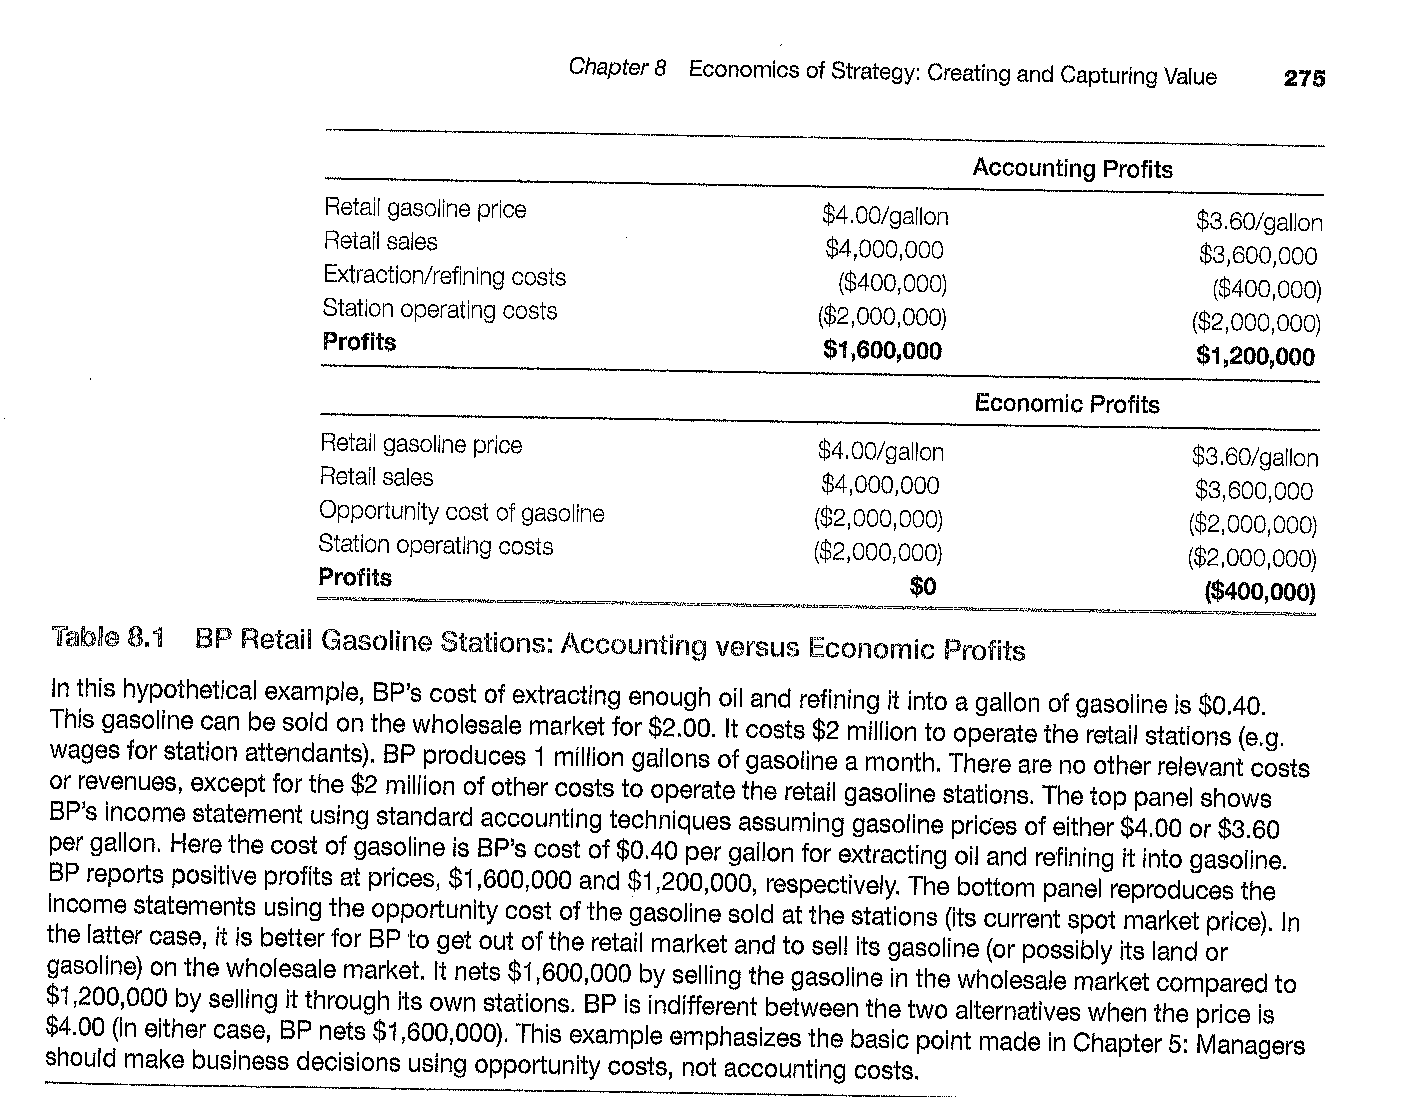
\includegraphics[width=0.7\linewidth]{BSZ_kap_8_2026/by_slide/slide_011/BSZ_kap_8_2026_slide_011_asset_01_image6.png}
  \caption{BSZ Table 8.1: BP Retail Gasoline Stations -- regnskapsmessig vs.\ økonomisk profitt. Ved \$3{,}60/gallon er accounting profit positiv men economic profit negativ. Aktiviteten bør outsources. [SLIDE -- BSZ kap.\ 8]}
\end{figure}

\subsection*{Illustrasjon -- market power-modellen (TikZ)}

\begin{figure}[h]
\centering
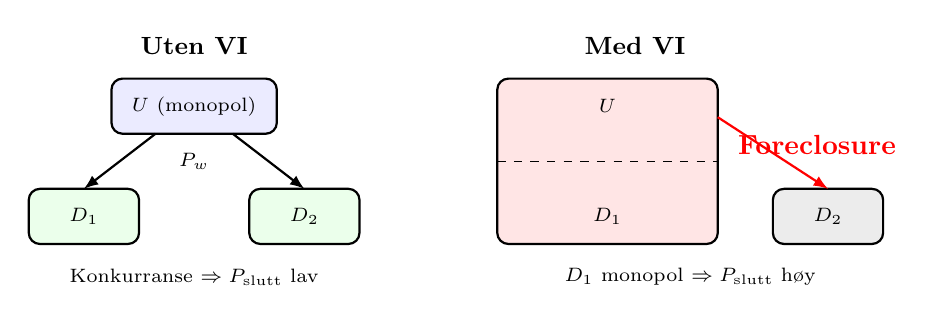
\begin{tikzpicture}[>=latex, scale=0.7, every node/.style={font=\scriptsize}]
  % Uten VI
  \node[font=\small\bfseries] at (3, 5.8) {Uten VI};
  \draw[thick, rounded corners, fill=blue!8] (1.5,4.2) rectangle (4.5,5.2);
  \node at (3,4.7) {$U$ (monopol)};
  \draw[thick, rounded corners, fill=green!8] (0,2.2) rectangle (2,3.2);
  \node at (1,2.7) {$D_1$};
  \draw[thick, rounded corners, fill=green!8] (4,2.2) rectangle (6,3.2);
  \node at (5,2.7) {$D_2$};
  \draw[->, thick] (2.3,4.2) -- (1,3.2);
  \draw[->, thick] (3.7,4.2) -- (5,3.2);
  \node at (3,3.7) {$P_w$};
  \node at (3,1.6) {Konkurranse $\Rightarrow P_{\text{slutt}}$ lav};
  % Med VI
  \begin{scope}[xshift=8cm]
  \node[font=\small\bfseries] at (3, 5.8) {Med VI};
  \draw[thick, rounded corners, fill=red!10] (0.5,2.2) rectangle (4.5,5.2);
  \node at (2.5,4.7) {$U$};
  \node at (2.5,2.7) {$D_1$};
  \draw[dashed] (0.5,3.7) -- (4.5,3.7);
  \draw[thick, rounded corners, fill=gray!15] (5.5,2.2) rectangle (7.5,3.2);
  \node at (6.5,2.7) {$D_2$};
  \draw[->, thick, red] (4.5,4.5) -- (6.5,3.2);
  \node[red, font=\bfseries] at (6.3,4.0) {Foreclosure};
  \node at (4,1.6) {$D_1$ monopol $\Rightarrow P_{\text{slutt}}$ høy};
  \end{scope}
\end{tikzpicture}
\caption{Vertikal integrasjon for market power: $U$--$D_1$ integrerer og stenger ute $D_2$ via foreclosure. [SLIDE/BOK -- BSZ kap.\ 19]}
\end{figure}

\subsection*{Real-world eksempler}

\textbf{Eks.~1 -- De Beers (diamantindustrien).}\quad [EKS]
De Beers kontrollerte historisk $\sim$80\% av verdens rådiamantproduksjon (oppstrøms monopol) og integrerte nedstrøms via Central Selling Organisation for distribusjon. Uavhengige slipere og forhandlere ble tvunget til å kjøpe via De Beers eller ble stengt ute (\emph{foreclosure}). Resultatet var kontrollert tilbud og kunstig høye diamantpriser i tiår. Modellen for VI og market power beskriver mekanismen presist.

\textbf{Eks.~2 -- Mærsk/APM Terminals, sammenligning.}\quad [EKS/CASE]
Mærsk integrerte nedstrøms i terminal-operasjoner (APM Terminals) -- men primærmotivet var \emph{effektivitet} (sikre havnekapasitet, redusere holdetid) snarere enn foreclosure av rivaler. EU-kommisjonen har vurdert om integrasjonen gir Mærsk urimelig konkurransefordel i rederibransjen, men godkjent fusjoner under vilkår om tredjepartstilgang. Sammenligningen med De Beers viser at VI kan ha ulike motiver: effektivitet (Mærsk) vs.\ rent-seeking (De Beers). Grensen er sentral for konkurranserett.

\subsection*{Kobling til Mærsk Power-to-X}
PtX illustrerer make-or-buy-beslutningen konkret: skal Mærsk produsere grønt hydrogen selv (integrere bakover i elektrolyse) eller kjøpe på markedet? Argumenter for integrasjon: spesifikt aktivum (elektrolyseanlegg tilpasset Mærsks spesifikasjon), usikkerhet om hydrogenmarkedets modenhet, beskyttelse av teknologisk forsprang. Argumenter for outsourcing: manglende kjernekompetanse i energiproduksjon, skalafordeler hos dedikerte energiselskaper. Økonomisk profitt-analysen er avgjørende: regnskapet kan vise positiv margin på intern produksjon, men alternativkostnaden (kapital bundet i elektrolyseanlegg i stedet for i rederidrift) kan gjøre $\pi_{\text{economic}}<0$. [CASE]

\subsection*{Fallgruber}
\begin{itemize}\setlength{\itemsep}{2pt}
\item Glemme å definere \emph{economic} vs.\ \emph{accounting} profit eksplisitt -- spørsmålet nevner det direkte.
\item Bare ramse opp fordeler/ulemper uten å forankre i transaksjonskostnadsteori (Coase/Williamson).
\item Forveksle Q11 med Q12: Q11 handler om \emph{Boundaries of the Firm} og \emph{market power}; Q12 handler om de tre \emph{kontraktproblemene} (hold-up, free-rider, double markup).
\item Glemme modellen for market power -- spørsmålet ber eksplisitt om den.
\item Ignorere Chicago School-kritikken av market power-argumentet.
\item Tegne market power-modellen feil: det er oppstrøms monopol + nedstrøms foreclosure, ikke omvendt.
\end{itemize}

\subsection*{Håndskrivbar disposisjon (15-min forberedelse)}
\begin{itemize}\setlength{\itemsep}{2pt}
\item \textbf{Tese:} Firmaets grenser bestemt av transaksjonskost vs.\ byråkratikost; VI lønner seg ved spesifikke aktiva, usikkerhet, markedsmakt.
\item \thref{boundaries-of-the-firm}{Boundaries of the Firm}: Coase, Williamson, eierskap = residuell kontroll (GHM).
\item \thref{accounting-vs-economic-profit}{Acc.\ vs.\ econ.\ profit}: $\pi_{\text{econ}} = R - C_{\text{exp}} - C_{\text{opp}}$. BP-eksempel Table 8.1.
\item \textbf{Fordeler outsourcing:} markedsdisiplin, skala, fleksibilitet, sterkere insentiver.
\item \textbf{Fordeler VI:} hold-up eliminert, kontroll, koordinasjon, IP-beskyttelse, market power.
\item \thref{vertical-integration-market-power}{Market power-modell}: $U$ monopol $\to$ integrerer $D_1$ $\to$ foreclosure av $D_2$. Figur.
\item Chicago-kritikk: VI tilfører ikke ny markedsmakt hvis $U$ allerede kan ekstrahere via inputpris.
\item Eks.\ 1: De Beers (foreclosure). Eks.\ 2: Mærsk/APM Terminals (effektivitet vs.\ foreclosure).
\item Case: Mærsk PtX -- make-or-buy for elektrolyse; econ.\ profit-analyse.
\item Søyle: \SOne\ (eierskap, beslutningsrett) + \STwo\ (profittbegrep).
\end{itemize}

% !TEX root = ../main.tex
\section{Q12: Vertikal integrasjon vs.\ outsourcing -- hold-up, free-rider, double markup}\label{q:12}

\begin{quote}
\emph{Præsenter begreberne vertikal integration og outsourcing / market transactions og redegør for principielle fordele og ulemper ved de respektive organiseringsalternativer. Diskuter i denne forbindelse kontraktmæssige aspekter af interaktion mellem virksomheden og dens leverandører/distributører -- herunder: hold-up problemer, free-rider problemer, double markup problemer.}
\end{quote}

\subsection*{Svar (kort)}
Vertikal integrasjon og outsourcing er to ytterpunkter på et organiseringskontinuum; fordeler og ulemper følger av \thref{costly-contracting}{costly contracting} og informasjonsasymmetri. De tre kontraktproblemene -- hold-up, free-rider og double markup -- er distinkte årsaker til at markedskontrakter mellom uavhengige parter feiler, og hver peker mot vertikal integrasjon (eller spesifikke kontraktsdesign) som løsning. Hold-up skyldes relasjonsspesifikke investeringer, free-riding skyldes positive eksternaliteter mellom distributører, og double markup skyldes uavhengig prissetting av to suksessive monopolister. [SLIDE]

\subsection*{Relevante teorier (kort)}

\paragraph{\thref{vertical-integration-outsourcing}{Vertikal integrasjon og outsourcing (bredt)}\quad\SOne/\SThree}
Outsourcing gir markedsdisiplin, skalafordeler, fleksibilitet og sterkere insentiver. Integrasjon gir kontroll, koordinasjon, IP-beskyttelse og eliminering av kontraktproblemer. Valget er en trade-off mellom transaksjonskostnader i markedet og \thref{agency-costs}{agency costs} internt. Se Q11 for koblingen til Boundaries of the Firm, eierskap og market power. [SLIDE]

\paragraph{\thref{hold-up-problem}{Hold-up-problemet}\quad\SOne/\SThree}
Når en part investerer i \emph{relasjonsspesifikke aktiva} -- altså investeringer som er mye mer verdt i akkurat denne relasjonen enn andre steder (lav alternativverdi) -- kan motparten i ettertid (\emph{ex post}) reforhandle og kapre \emph{quasi-renter}: differansen $V - V_0$ mellom verdien i relasjonen ($V$) og verdien i nest-beste anvendelse ($V_0$). Konsekvens: rasjonelle parter forutser dette og underinvesterer i forkant (\emph{ex ante}). Løsninger: vertikal integrasjon (samme eier eliminerer reforhandling), langsiktige kontrakter, gjensidig avhengighet (hver part har egne spesifikke aktiva som ``gissel''), og reputasjon. Klassisk eksempel: GM--Fisher Body på 1920-tallet. Williamsons fem typer asset specificity (site -- lokasjon; physical -- spesialisert utstyr; human -- spesialisert kompetanse; dedicated -- kapasitet bygget kun for én kunde; temporal -- tidssensitivitet) bestemmer hold-up-risikoen. [SLIDE/BOK]

\paragraph{\thref{free-rider-problem}{Free-rider-problemet (nedstrøms)}\quad\SThree}
Uavhengige distributører underinvesterer i service og markedsføring fordi gevinsten fanges av konkurrerende forhandlere (\emph{inter-dealer free-riding}). Klassisk eksempel: kunden bruker high-service-forhandleren (stort showroom, god rådgivning) til å bestemme seg, og kjøper deretter billigere hos en discount-forhandler som ikke har slike kostnader. Dette kalles \emph{showrooming}: kunden ``viser fram'' produktet i én butikk, kjøper i en annen. Resultat: ingen vil bygge showroomet -- service-nivået kollapser. Løsninger: vertikal integrasjon (produsenten eier distribusjonen selv), franchise med servicekrav, eksklusive territorier (én forhandler per geografisk område), og \emph{RPM} (\emph{Resale Price Maintenance} -- produsenten setter en minste videresalgspris og forbyr priskonkurranse nedstrøms, slik at margingrunnlaget for å yte service bevares). [BOK]

\begin{tcolorbox}[colback=blue!4, colframe=blue!50!black, boxrule=0.4pt, arc=2pt, left=6pt, right=6pt, top=4pt, bottom=4pt]
\textbf{Intuisjon:} Free-rider = du høster gevinsten av andres investering uten å bidra. McDonald's-franchisee på Gardermoen investerer ikke i kvalitet -- eksternalitet = påfører andre kostnad; free-rider = tar andres gevinst. Begge gir underinvestering -- ulik mekanisme.
\end{tcolorbox}

\paragraph{\thref{double-markup-problem}{Double markup-problemet}\quad\SOne}
To suksessive monopolister i samme verdikjede setter prisen uavhengig av hverandre, og hver legger på sin egen markup (påslag). Resultat: \emph{dobbelt} markup -- oppstrøms margin pluss nedstrøms margin -- gir sluttforbrukerpris høyere og kvantum lavere enn det som er optimalt for verdikjeden samlet. Talleksempel: marginalkostnad $c=20$, oppstrømsprisen $P_w=60$ (45 \% markup), sluttpris $P_{\text{slutt}}=80$, kvantum $Q=20$. Hvis de to integrerer (én aktør, én markup): $P=60$, $Q=40$ -- +33\% profitt og +100\% kvantum. Kontraktuelle alternativer som unngår full integrasjon: \emph{two-part tariff} (en fast avgift pluss enhetspris -- f.eks.\ engangsgebyr + lav pris per enhet), \emph{franchise fee} (engangsbeløp for retten til å selge), eller RPM (Resale Price Maintenance -- produsenten setter videresalgsprisen direkte). Forutsetter monopol i begge ledd; med konkurranse nedstrøms forsvinner $D$s markup uansett. [SLIDE]

\subsection*{Illustrasjoner fra forelesning}

\begin{figure}[H]
  \centering
  
\includegraphics[width=0.55\linewidth]{BSZ_kap_10_2026/by_slide/slide_017/BSZ_kap_10_2026_slide_017_asset_01_image7.jpeg}
  \caption{Tautrekking mellom parter -- illustrerer hold-up-problemet: når begge parter har investert, oppstår forhandlingskonflikt om quasi-renter. (BSZ kap.\ 10, slide 17) [SLIDE]}
\end{figure}

\begin{figure}[H]
  \centering
  
\includegraphics[width=0.45\linewidth]{BSZ_kap_9_2026/by_slide/slide_015/BSZ_kap_9_2026_slide_015_asset_01_image4.jpeg}
  \caption{Oppvasken ingen tar -- illustrerer free-rider-problemet: alle nyter godt av at jobben gjøres, men ingen vil bære kostnaden. (BSZ kap.\ 9, slide 15) [SLIDE]}
\end{figure}

\subsection*{Illustrasjon -- de tre kontraktproblemene}

\begin{center}
\renewcommand{\arraystretch}{1.2}
\begin{tabular}{@{}p{2.8cm}p{3.5cm}p{3.5cm}p{3.5cm}@{}}
\toprule
 & \textbf{Hold-up} & \textbf{Free-rider} & \textbf{Double markup} \\
\midrule
\textbf{Kilde} & Spesifikke investeringer & Positiv eksternalitet mellom dist. & Suksessive monopolister \\
\textbf{Mekanisme} & Reforhandling ex post & Underinvestering i service & Dobbel prispåslag \\
\textbf{Konsekvens} & Underinvestering ex ante & Merkevare eroderes & For høy pris, for lavt $Q$ \\
\textbf{VI-løsning} & Felles eierskap & Eie distribusjon & Fjerne én markup \\
\textbf{Kontraktsløsning} & Langsiktig k., penalty & Franchise, eksklusive terr. & Two-part tariff, RPM \\
\bottomrule
\end{tabular}
\end{center}
\textit{Tabell: Sammenligning av de tre kontraktproblemene og deres løsninger. [SLIDE/BOK]}

\subsection*{Illustrasjon -- double markup (grafisk)}

\begin{figure}[H]
\centering
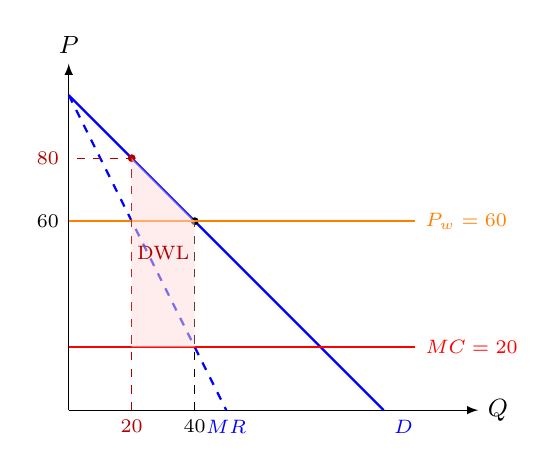
\begin{tikzpicture}[>=latex, scale=0.8, every node/.style={font=\small}]
  \draw[->] (0,0) -- (6.5,0) node[right] {$Q$};
  \draw[->] (0,0) -- (0,5.5) node[above] {$P$};
  \draw[thick, blue] (0,5) -- (5,0) node[below right] {\scriptsize $D$};
  \draw[thick, blue, dashed] (0,5) -- (2.5,0) node[below] {\scriptsize $MR$};
  \draw[thick, red] (0,1.0) -- (5.5,1.0) node[right] {\scriptsize $MC=20$};
  % Integrert
  \filldraw[black] (2.0,3.0) circle (1.5pt);
  \draw[dashed] (2.0,0) -- (2.0,3.0) -- (0,3.0);
  \node[below] at (2.0,0) {\scriptsize $40$};
  \node[left] at (0,3.0) {\scriptsize $60$};
  % Double markup
  \draw[thick, orange] (0,3.0) -- (5.5,3.0) node[right] {\scriptsize $P_w=60$};
  \filldraw[red!70!black] (1.0,4.0) circle (1.5pt);
  \draw[dashed, red!70!black] (1.0,0) -- (1.0,4.0) -- (0,4.0);
  \node[below, red!70!black] at (1.0,0) {\scriptsize $20$};
  \node[left, red!70!black] at (0,4.0) {\scriptsize $80$};
  % DWL
  \fill[red!15, opacity=0.5] (1.0,4.0) -- (2.0,3.0) -- (2.0,1.0) -- (1.0,1.0) -- cycle;
  \node[font=\scriptsize, red!70!black] at (1.5,2.5) {DWL};
\end{tikzpicture}
\caption{Double markup: uintegrert $P=80, Q=20$ (rødt) vs.\ integrert $P=60, Q=40$ (svart). [BOK]}
\end{figure}

\subsection*{Real-world eksempler}

\textbf{Eks.~1 -- IKEA og leverandørrelasjoner (hold-up og kontraktsdesign).}\quad [EKS]
IKEA designer produkter som krever \emph{dedikerte} produksjonslinjer hos leverandører i Øst-Europa og Asia (physical + dedicated asset specificity). For å unngå hold-up bruker IKEA flerårige rammeavtaler med volum-garantier, kvalitetsinspeksjoner (monitoring) og gradvis diversifisering av leverandørbasen. IKEA integrerer \emph{ikke} vertikalt i produksjon -- kontraktsløsningen er billigere enn integrasjon fordi produktene er modulære (moderat spesifisitet).

\textbf{Eks.~2 -- McDonald's (free-rider og franchising), sammenligning.}\quad [EKS]
McDonald's løser free-rider-problemet gjennom \emph{franchising} med strenge servicekrav: kvalitetsstandarder, renhold, menyer og opplæring kontrolleres sentralt. Franchisetaker som leverer dårlig kvalitet skader merket (free-riding) og mister lisensen. Kontrast med IKEA: McDonald's nedstrømsproblem (distributør free-rider) løses med franchise, mens IKEAs oppstrømsproblem (leverandør hold-up) løses med rammeavtaler. Begge unngår full integrasjon fordi kontraktsdesign er tilstrekkelig -- men forutsetter effektiv monitoring.

\subsection*{Kobling til Mærsk Power-to-X}
PtX-verdikjeden illustrerer alle tre kontraktproblemene: [CASE]
\begin{itemize}\setlength{\itemsep}{2pt}
\item \textbf{Hold-up:} Elektrolyseanlegg bygget til Mærsks spesifikasjon er et spesifikt aktivum. Leverandøren (f.eks.\ Siemens Energy) kan holdes opp etter investering -- Mærsks løsning: milestone-betalinger, performance guarantees, step-in-rettigheter.
\item \textbf{Free-rider:} Mærsk samarbeider med andre rederier i bransjeinitiativ for grønt drivstoff. Uten forpliktende kontrakter kan partnere free-ride på Mærsks investeringer i infrastruktur.
\item \textbf{Double markup:} Hvis elektrolyseprodusent og e-metanol-produsent begge har markedsmakt, kan dobbel markup drive opp drivstoffprisen. Mærsks interesse i bakoverintegrasjon til elektrolyse eliminerer dette leddet.
\end{itemize}

\subsection*{Fallgruber}
\begin{itemize}\setlength{\itemsep}{2pt}
\item Forveksle Q12 med Q11: Q12 handler om \emph{kontraktproblemer}; Q11 handler om \emph{Boundaries of the Firm} og \emph{market power}.
\item Kun beskrive VI-fordeler uten å nevne kontraktsalternativer (franchise, two-part tariff, RPM).
\item Forveksle hold-up (ex post reforhandling) med moral hazard (skjult handling) -- overlappende men distinkte.
\item Glemme double markup-tallet: vis det numeriske eksemplet ($Q: 20\to 40$, $\pi: 1200\to 1600$).
\item Ikke nevne asset specificity-typene ved hold-up -- Williamson krever det.
\item Behandle free-rider som generelt kollektiv handlingsproblem -- i VI-konteksten er det spesifikt om distributører.
\end{itemize}

\FloatBarrier
\subsection*{Håndskrivbar disposisjon (15-min forberedelse)}
\begin{itemize}\setlength{\itemsep}{2pt}
\item \textbf{Tese:} Tre kontraktproblemer (hold-up, free-rider, double markup) forklarer når outsourcing feiler og VI lønner seg.
\item \thref{vertical-integration-outsourcing}{VI vs.\ outsourcing}: fordeler/ulemper kort (markedsdisiplin vs.\ kontroll).
\item \textbf{Hold-up:} spesifikke aktiva $\Rightarrow$ quasi-rente approprieres $\Rightarrow$ underinvestering. 5 typer asset specificity. Løsning: VI, langsiktig kontrakt, mutual hostage.
\item \textbf{Free-rider:} distributør underinvesterer i service. Showrooming. Løsning: franchise, eksklusive terr., RPM.
\item \textbf{Double markup:} $c=20, P_w=60, P=80, Q=20$ vs.\ integrert $P=60, Q=40$. Løsning: VI, two-part tariff.
\item Tabell: sammenligning av de tre problemene (kilde, mekanisme, løsning).
\item Eks.\ 1: IKEA (hold-up, rammeavtaler). Eks.\ 2: McDonald's (free-rider, franchise).
\item Case: Mærsk PtX -- alle tre problemene representert.
\item Søyle: \SOne\ (eierskap/kontroll) + \SThree\ (insentivdesign for leverandører/distributører).
\end{itemize}

% !TEX root = ../main.tex
\section{Q13: Regulering -- offentlig indgriben, branche-profit og political support}\label{q:13}

\begin{quote}
\emph{Præsentér økonomisk-teoretiske argumenter for hvornår offentlig indgriben i og regulering af markeder er hensigtsmæssig/anbefalelsesværdig samt for forudsætningerne bag disse argumenter. I forlængelse heraf ønskes en konkret præsentation af og redegørelse for modellen til beskrivelse af regulerede priser på baggrund af branche-profit-funktioner og political support-funktioner.}
\end{quote}

\subsection*{Svar (kort)}
Offentlig indgriben er hensigtsmæssig ved fire typer markedssvikt: naturlig monopol, eksternaliteter, offentlige goder og informasjonsasymmetri -- men kun under forutsætning av at reguleringsgevinsten overstiger reguleringsomkostningerne (government failure, regulatory capture). BSZ kap.\ 21-modellen viser at den regulerede prisen $P^*$ bestemmes der regulatoren (politikeren) maksimerer \emph{political support} $S(\pi, CS)$ -- en funksjon av brancheprofitt og konsumentoverskudd. Resultatet: $P^*$ ligger mellom $P^{MC}$ og $P^M$, avhengig av de relative lobbyingsressursene. [SLIDE]

\subsection*{Relevante teorier (kort)}

\paragraph{\thref{market-failure-regulation}{Markedssvikt og regulering}\quad\SOne}
Fire argumenter: (1) \textbf{Naturlig monopol}: fallende $AC$ $\Rightarrow$ én produsent billigst, men $P>MC$ uten konkurranse. Løsning: prisregulering, konsesjoner. (2) \textbf{Eksternaliteter} (\thref{externalities}{jf.\ Q07}): handlinger med uforprisede konsekvenser for tredjepart. Løsning: Pigou-skatt, kvoter. (3) \textbf{Offentlige goder}: ikke-rivaliserende, ikke-ekskluderbare $\Rightarrow$ free-riding. Løsning: offentlig tilbud. (4) \textbf{Informasjonsasymmetri} (\thref{adverse-selection}{adverse selection}): lemons, markedskollaps. Løsning: informasjonsplikt, sertifisering. Forutsetter at regulatoren er bedre informert og mer effektiv enn markedet -- noe som ikke alltid stemmer. [SLIDE/BOK]

\paragraph{\thref{regulated-pricing-model}{Regulated pricing-modellen (political support)}\quad\SOne}
BSZ kap.\ 21/Peltzman (1976): regulatoren maksimerer $S(\pi(P), CS(P))$. Brancheprofitt $\pi(P)$ er invers-U (null ved $P=AC$, topp ved $P^M$). Konsumentoverskudd $CS(P)$ er fallende. FOC: marginal politisk gevinst fra bransje ($\partial S/\partial \pi \cdot \pi'$) = marginal politisk kostnad fra konsumenter ($-\partial S/\partial CS \cdot CS'$). $P^*$ mellom $P^{MC}$ og $P^M$. Komparativ statikk: sterkere bransjelobby $\Rightarrow$ $P^*$ mot $P^M$; sterkere konsumentpress $\Rightarrow$ $P^*$ mot $P^{MC}$. [SLIDE/BOK]

\subsection*{Grafisk modell -- regulated pricing}

\begin{figure}[h]
\centering
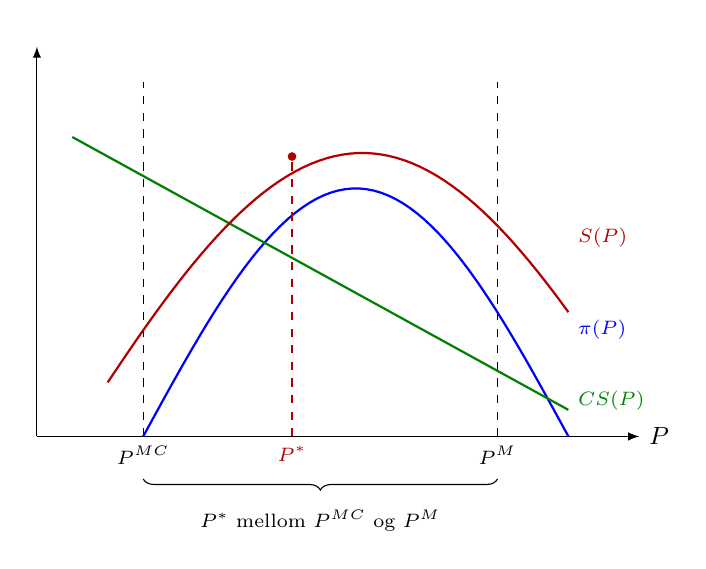
\begin{tikzpicture}[>=latex, scale=0.9, every node/.style={font=\small}]
  \draw[->] (0,0) -- (8.5,0) node[right] {$P$};
  \draw[->] (0,0) -- (0,5.5) node[above] {};
  % MC og PM
  \draw[dashed] (1.5,0) -- (1.5,5.0);
  \node[below] at (1.5,0) {\scriptsize $P^{MC}$};
  \draw[dashed] (6.5,0) -- (6.5,5.0);
  \node[below] at (6.5,0) {\scriptsize $P^{M}$};
  % pi(P)
  \draw[thick, blue, domain=1.5:7.5, samples=60]
    plot (\x, {3.5*sin((\x-1.5)*30)});
  \node[blue, right] at (7.5,1.5) {\scriptsize $\pi(P)$};
  % CS(P)
  \draw[thick, green!50!black, domain=0.5:7.5, samples=40]
    plot (\x, {4.5-0.55*\x});
  \node[green!50!black, right] at (7.5,0.5) {\scriptsize $CS(P)$};
  % S(P)
  \draw[thick, red!70!black, domain=1.0:7.5, samples=60]
    plot (\x, {4.0*sin((\x-0.5)*22)});
  \node[red!70!black, right] at (7.5,2.8) {\scriptsize $S(P)$};
  % P*
  \draw[thick, dashed, red!70!black] (3.6,0) -- (3.6,4.0);
  \node[below, red!70!black, font=\bfseries] at (3.6,0) {\scriptsize $P^{*}$};
  \filldraw[red!70!black] (3.6,3.95) circle (1.5pt);
  % Brace
  \draw[decorate, decoration={brace, amplitude=4pt, mirror}] (1.5,-0.6) -- (6.5,-0.6);
  \node[below, font=\scriptsize] at (4.0,-0.9) {$P^{*}$ mellom $P^{MC}$ og $P^{M}$};
\end{tikzpicture}
\caption{\textbf{Regulated pricing-modellen.} $\pi(P)$ (blå) topper ved monopolpris; $CS(P)$ (grønn) er fallende; $S(P)$ (rød) maksimeres ved $P^*$ mellom $P^{MC}$ og $P^M$. Regulatoren balanserer bransje- og konsumentinteresser. [BOK -- BSZ kap.\ 21]}
\end{figure}

\subsection*{De fire markedssviktene -- oversikt}

\begin{center}
\renewcommand{\arraystretch}{1.15}
\begin{tabular}{@{}p{3.0cm}p{3.5cm}p{3.0cm}p{3.5cm}@{}}
\toprule
\textbf{Svikt} & \textbf{Problem} & \textbf{Verktøy} & \textbf{Forutsætning} \\
\midrule
Naturlig monopol & $P>MC$, underprod. & Priskontroll & Fallende $AC$ \\
Eksternaliteter & Over-/underprod. & Pigou, kvoter & Tredjepartseffekt \\
Offentlige goder & Free-riding & Offentlig tilbud & Ikke-rival., ikke-ekskl. \\
Info.asymmetri & Lemons & Informasjonsplikt & Hidden info/action \\
\bottomrule
\end{tabular}
\end{center}

\subsection*{Real-world eksempler}

\textbf{Eks.~1 -- Norsk farmasiregulering.}\quad [EKS]
Statens legemiddelverk setter maksimale utsalgspriser (\emph{prisregulering}). Argumentet: naturlig monopol (patentbeskyttet legemiddel) + informasjonsasymmetri (pasienten kan ikke vurdere kvalitet). Prisen reflekterer political support-modellen: lavere enn USAs uregulerte priser (sterk konsumentinteresse, universell helseforsikring) men høyere enn generiske alternativ (bransjelobby for innovasjonsinsentiv). Forutsætningen er at regulatoren faktisk har bedre informasjon enn markedet -- kritikken er at industrien har informasjonsovertak og risikerer regulatory capture.

\textbf{Eks.~2 -- EU Emissions Trading System (ETS), sammenligning.}\quad [EKS]
ETS regulerer CO$_2$-utslipp (negativ eksternalitet) via kvotehandel -- en Pigou-mekanisme. Prisen ($\sim$50--80 EUR/tonn i 2024) er et politisk kompromiss mellom industriens profitt (høy kvotepris truer lønnsomhet) og konsumenter/klima (lav kvotepris gir for lite utslippsreduksjon). Sammenligningen med farmasiregulering: begge er political support-modellen i praksis, men med ulike markedssvikter (monopol vs.\ eksternalitet) og ulike verktøy (priskontroll vs.\ kvoter). I begge tilfeller avhenger $P^*$ av lobbyingsstyrke.

\subsection*{Kobling til Mærsk Power-to-X}
PtX mottar offentlige subsidier (EU Hydrogen Strategy, IPCEI) fordi grønt hydrogen produserer \emph{positive eksternaliteter} (klimareduksjon) som markedet underpriser. Reguleringsresponsen -- subsidie -- er korreksjonen for eksternaliteten. I tillegg er Mærsks PtX-satsing avhengig av at regulering av skipsdrivstoff (EU ETS Maritime, IMO) øker kostnaden ved fossil fuel (Pigou-skatt) og dermed gjør grønt alternativ kommersielt levedyktig. Political support-modellen forklarer hvorfor reguleringen er gradvis: skipsfartsbransjens lobby bremser innføringstakten, mens klimalobby presser den framover. [CASE]

\subsection*{Fallgruber}
\begin{itemize}\setlength{\itemsep}{2pt}
\item Glemme \emph{forudsætningerne} for at regulering er hensigtsmæssig -- sensor vil ha betingelsene, ikke bare argumentene.
\item Bare ramse opp de fire markedssviktene uten å forklare mekanismen (underproduksjon/overproduksjon/lemons).
\item Ignorere government failure, regulatory capture og Averch-Johnson -- regulering er ikke gratis.
\item Tegne modellen feil: $\pi(P)$ er \emph{invers-U}, ikke monotont stigende. $CS(P)$ er fallende, ikke stigende.
\item Glemme komparativ statikk: hva skjer med $P^*$ når lobbyingsstyrke endres?
\item Forveksle positiv analyse (``hva bestemmer regulert pris?'') med normativ (``hva bør regulert pris være?'') -- modellen er positiv (Peltzman), ikke normativ (Pigou).
\end{itemize}

\subsection*{Håndskrivbar disposisjon (15-min forberedelse)}
\begin{itemize}\setlength{\itemsep}{2pt}
\item \textbf{Tese:} Regulering hensigtsmæssig ved 4 markedssvikter, men betinget av at reguleringsgevinst > reguleringsomkostning. Modellen viser at $P^*$ er politisk kompromiss, ikke velferdsmaksimum.
\item \textbf{4 svikter:} (1) Naturlig monopol ($AC$ fallende). (2) Eksternaliteter (Pigou). (3) Offentlige goder (free-rider). (4) Info.asymmetri (lemons).
\item \textbf{Forutsætninger:} signifikant svikt, regulatoren informert, ikke capture.
\item \textbf{Modell:} $\pi(P)$ invers-U; $CS(P)$ fallende; $S(\pi, CS)$ maksimeres ved $P^*$. FOC: $\partial S/\partial\pi \cdot \pi' = -\partial S/\partial CS \cdot CS'$.
\item \textbf{Komparativ statikk:} sterkere lobby $\Rightarrow$ $P^*\to P^M$; sterkere konsument $\Rightarrow$ $P^*\to P^{MC}$.
\item \textbf{Kritikk:} government failure, capture (Stigler), AJ-overinvestering, Olsons kollektiv handling.
\item Eks.\ 1: Norsk farmasiregulering (monopol + info.asym.). Eks.\ 2: EU ETS (eksternalitet).
\item Case: Mærsk PtX -- subsidier for pos.\ eksternalitet + IMO-regulering som Pigou.
\item Søyle: \SOne\ (regulatoren allokerer rettigheter stat/marked).
\end{itemize}

% !TEX root = ../main.tex
\section{Q14: Informativeness-prinsippet -- kontrollerbarhed, risikodeling, presisjon, risikopræmie}\label{q:14}

\begin{quote}
\emph{Redegør for Informativeness-princippet i relation til design af kontrakter og kompensation. Følgende forhold og begreber forventes inddraget: a) kontrollerbarhed, b) risikodeling, c) målingers præcision, d) risikopræmie.}
\end{quote}

\subsection*{Svar (kort)}
Informativeness-prinsippet (Holmström 1979) sier at et signal $y$ bør inkluderes i kontrakten hvis og bare hvis det er statistisk informativt om agentens innsats -- dvs.\ at det endrer posterior for $e$ gitt det primære målet $Q$. Prinsippet binder de fire delspørsmålene sammen: (a) controllability er et \emph{spesialtilfelle} -- informativeness er bredere, fordi ukontrollerbare mål kan likevel være informative; (b) mer informative signaler forbedrer risikodelingen ved å senke effektiv støy; (c) presise mål (lav $\sigma^2$) er mer informative og bør vektes høyere ($\beta$ opp); (d) risikopremien $RP = \tfrac{r}{2}\beta^2\sigma^2$ synker når signaler filtrerer bort støy. [SLIDE]

\subsection*{Relevante teorier (kort)}

\paragraph{\thref{informativeness-principle}{Informativeness-prinsippet}\quad\STwo/\SThree}
Holmströms tilstrekkelighets\-kriterium: inkludér signal $y$ i kontrakten $\Leftrightarrow$ $f(Q|e,y)\neq f(Q|e)$ for noen $(Q,y)$. Kontrakt utvides til $W=W_0+\beta_1 Q + \beta_2 y$. Effekten: lavere effektiv varians $\sigma^2_{\text{eff}} < \sigma^2$, dermed lavere risikopremie for gitt insentivnivå, eller sterkere insentiver for gitt risikopremie. Sufficient statistic-poenget: hvis $Q$ allerede fanger all informasjon om $e$, skal $y$ \emph{ikke} brukes. [SLIDE]

\paragraph{\thref{controllability-principle}{(a) Controllability-prinsippet}\quad\STwo}
Lederen skal kun evalueres på det hun kontrollerer. Men informativeness \emph{generaliserer} dette: et ukontrollerbart mål (f.eks.\ bransjeavkastning, oljepris) kan \emph{forbedre} kontrakten hvis det filtrerer ut felles sjokk fra agentens mål. Controllability er nødvendig i snever forstand (ikke straff for eksogene sjokk), men informative mål som er ukontrollerbare er likevel verdifulle som filtreringsinstrumenter. [SLIDE]

\paragraph{\thref{risk-sharing}{(b) Risikodeling}\quad\SThree}
Risikoavers agent + risikonøytral prinsipal $\Rightarrow$ first-best er fast lønn. Men \thref{moral-hazard}{moral hazard} krever $\beta>0$ for å vri innsats $\Rightarrow$ agenten bærer risiko $\Rightarrow$ risikopremie. Informativeness forbedrer trade-offen: med mer informative signaler kan man oppnå \emph{samme} innsatsnivå med \emph{lavere} risiko for agenten, eller \emph{høyere} innsats med \emph{samme} risiko. Risikodelingen blir Pareto-bedre. [SLIDE]

\paragraph{\thref{incentive-coefficient}{(c) Målingers presisjon og (d) risikopremie}\quad\STwo/\SThree}
Presisjon = invers varians: høy presisjon $\Rightarrow$ lav $\sigma^2$ $\Rightarrow$ høyere $\beta^*$ (\thref{incentive-coefficient}{$\beta^* = 1/(1+r\sigma^2 c''/\alpha^2)$}). Risikopremien $RP = \tfrac{r}{2}\beta^2\sigma^2$ er stigende i støy -- upresise mål er dyre å bruke som insentivgrunnlag. Informativeness-prinsippet sier: legg til signaler som øker presisjonen (senker effektiv $\sigma^2$), og unngå signaler som bare tilfører støy. Relative prestasjonsmål (\thref{absolute-vs-relative-performance}{rTSR}) er det viktigste eksemplet: peer-avkastning filtrerer felles markedssjokk og øker presisjonen av det individuelle signalet. [SLIDE/BOK]

\subsection*{Illustrasjon -- informativeness-prinsippet}

\begin{figure}[h]
\centering
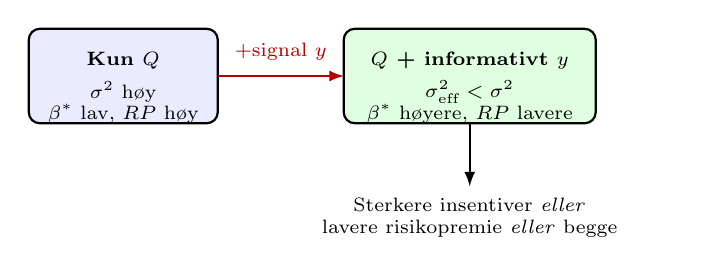
\begin{tikzpicture}[>=latex, scale=0.8, every node/.style={font=\small}]
  % Q bare
  \draw[thick, rounded corners, fill=blue!8] (0,3.0) rectangle (3.0,4.5);
  \node[font=\bfseries\scriptsize] at (1.5,4.0) {Kun $Q$};
  \node[font=\scriptsize] at (1.5,3.5) {$\sigma^2$ høy};
  \node[font=\scriptsize] at (1.5,3.15) {$\beta^*$ lav, $RP$ høy};
  % Q + y
  \draw[thick, rounded corners, fill=green!12] (5.0,3.0) rectangle (9.0,4.5);
  \node[font=\bfseries\scriptsize] at (7.0,4.0) {$Q$ + informativt $y$};
  \node[font=\scriptsize] at (7.0,3.5) {$\sigma^2_{\text{eff}} < \sigma^2$};
  \node[font=\scriptsize] at (7.0,3.15) {$\beta^*$ høyere, $RP$ lavere};
  % Arrow
  \draw[->, thick, red!70!black] (3.0,3.75) -- (5.0,3.75);
  \node[above, font=\scriptsize, red!70!black] at (4.0,3.85) {+signal $y$};
  % Resultat
  \draw[->, thick] (7.0,3.0) -- (7.0,2.0);
  \node[font=\scriptsize, text width=5cm, align=center] at (7.0,1.5) {Sterkere insentiver \emph{eller}\\lavere risikopremie \emph{eller} begge};
\end{tikzpicture}
\caption{Informativeness: tillegg av informativt signal $y$ senker effektiv $\sigma^2$ og forbedrer insentiv-risiko-trade-offen. [SLIDE/BOK]}
\end{figure}

\subsection*{Kobling mellom de fire delspørsmålene}

\begin{center}
\renewcommand{\arraystretch}{1.15}
\begin{tabular}{@{}p{3.2cm}p{4.5cm}p{5.5cm}@{}}
\toprule
\textbf{Begrep} & \textbf{Rolle i modellen} & \textbf{Kobling til informativeness} \\
\midrule
(a) Kontrollerbarhet & Mål det agenten kan styre & Informativeness er \emph{bredere}: ukontrollerbare mål kan likevel filtrere støy \\
(b) Risikodeling & $\beta>0 \Rightarrow$ agenten bærer risiko & Bedre signaler $\Rightarrow$ bedre risikodeling for gitt innsats \\
(c) Presisjon & Invers varians av signal & Presise mål er mer informative $\Rightarrow$ høyere $\beta^*$ \\
(d) Risikopremie & $RP = \tfrac{r}{2}\beta^2\sigma^2$ & Lavere effektiv $\sigma^2 \Rightarrow$ lavere $RP$ \\
\bottomrule
\end{tabular}
\end{center}

\subsection*{Slide-figur fra BSZ kap.\ 15}

\begin{figure}[h]
  \centering
  
\includegraphics[width=0.55\linewidth]{BSZ_kap_15_2026/by_slide/slide_014/BSZ_kap_15_2026_slide_014_asset_01_image3.png}
  \caption{Principal-agent-modellens notasjon fra BSZ kap.\ 15: $Q=\alpha e + \mu$, $W=W_0+\beta Q$. Informativeness-prinsippet utvider denne rammen med tilleggssignaler. [SLIDE -- BSZ kap.\ 15, slide 14]}
\end{figure}

\subsection*{Real-world eksempler}

\textbf{Eks.~1 -- Equinor CEO-kompensasjon (relativ Total Shareholder Return).}\quad [EKS]
Equinors LTI-program bruker \emph{relative TSR} mot en peer-gruppe av internasjonale energiselskaper (Shell, BP, TotalEnergies). Oljepris er et ukontrollerbart signal -- men det er \emph{informativt}: ved å trekke fra peer-gruppens avkastning filtreres felles oljeprisssjokk ut, og bonusen reflekterer den delen av avkastningen som skyldes konsernsjefens beslutninger. Informativeness-prinsippet er direkte grunnlaget: peer-TSR er et informativt signal ($y$) som senker effektiv $\sigma^2$ og tillater sterkere insentiver ($\beta$) uten uakseptabel risikopremie.

\textbf{Eks.~2 -- Norsk sykehuslege (kun subjektive mål), sammenligning.}\quad [EKS]
En sykehuslege evalueres i praksis kun subjektivt (avdelingsleders helhetsvurdering). Pasientutfall (helbredelse, overlevelse) er et upresist mål ($\sigma^2$ enorm -- avhenger av pasientens helsetilstand, komorbiditet). Informativeness-prinsippet tilsier at man \emph{bør} legge til informative signaler: prosessmål (etterlevelse av protokoller), volumjusterte utfallsmål, peer-sammenligning (case-mix-justert dødelighet). Men informasjonskostnaden er høy, og multitasking-problemet gjør at sterke insentiver på målt dimensjon vrir bort fra umålt omsorgskvalitet. Kontrasten med Equinor: i energibransjen er signalene (aksjekurs, oljepris) billige og informative; i helsesektoren er de dyre og upresise -- forskjellen forklarer ulik kontraktsdesign.

\subsection*{Kobling til Mærsk Power-to-X}
PtX-divisionens ledelse illustrerer alle fire aspekter: [CASE]
\begin{itemize}\setlength{\itemsep}{2pt}
\item \textbf{(a) Kontrollerbarhet:} Lederen kontrollerer prosjektgjennomføring men ikke elpris eller H$_2$-etterspørsel.
\item \textbf{(b) Risikodeling:} Stor $\sigma^2$ fra eksogene markeder $\Rightarrow$ lav $\beta$ på topplinjeresultat for å begrense risikopremie.
\item \textbf{(c) Presisjon:} Milestones (FID, anlegg ferdig, OPEX-budsjett) er presise og kontrollerbare $\Rightarrow$ kan bære høyere $\beta$.
\item \textbf{(d) Risikopremie:} Ved å bruke milestones + peer-benchmark (Ørsted, Air Liquide) senkes $\sigma^2_{\text{eff}}$ $\Rightarrow$ lavere $RP$.
\end{itemize}

\subsection*{Fallgruber}
\begin{itemize}\setlength{\itemsep}{2pt}
\item Presentere de fire begrepene som uavhengige -- de bindes sammen av informativeness-prinsippet.
\item Forveksle informativeness med controllability -- informativeness er \emph{bredere}; ukontrollerbare mål kan være informative.
\item Glemme sufficient statistics-poenget: ikke alle signaler er nyttige; noen tilfører bare støy.
\item Ikke nevne formelen: $\beta^* = 1/(1+r\sigma^2 c''/\alpha^2)$ -- den kobler presisjon og risikopremie direkte.
\item Bare abstrakt teori uten eksempel på relative mål (rTSR, peer-justering).
\item Glemme multitasking-begrensningen (Holmström--Milgrom): sterke insentiver på informative men ensidige mål vrir innsats.
\end{itemize}

\subsection*{Håndskrivbar disposisjon (15-min forberedelse)}
\begin{itemize}\setlength{\itemsep}{2pt}
\item \textbf{Tese:} Informativeness-prinsippet (Holmström 1979) er det overordnede rammeverket; (a)--(d) er konsekvenser/aspekter av det.
\item \textbf{Definisjon:} $y$ informativt $\Leftrightarrow$ endrer posterior for $e$ gitt $Q$. Sufficient statistic: inkluder $y$ \emph{bare} hvis det tilfører informasjon.
\item \textbf{(a) Kontrollerbarhet:} spesialtilfelle; informativeness er bredere (ukontrollerbare mål kan filtrere).
\item \textbf{(b) Risikodeling:} bedre signaler $\Rightarrow$ Pareto-bedre risk-sharing for gitt innsats.
\item \textbf{(c) Presisjon:} lav $\sigma^2$ $\Rightarrow$ høyere $\beta^*$. Formel: $\beta^*=1/(1+r\sigma^2 c''/\alpha^2)$.
\item \textbf{(d) Risikopremie:} $RP=\tfrac{r}{2}\beta^2\sigma^2$; lavere eff.\ $\sigma^2 \Rightarrow$ lavere $RP$.
\item \textbf{Kobling:} tabell som knytter a-b-c-d til informativeness.
\item \textbf{Hovedeksempel:} Relativ TSR (rTSR) -- peer-signal filtrerer markedssjokk.
\item Eks.\ 1: Equinor CEO + rTSR. Eks.\ 2: Norsk sykehuslege (upresise mål, subjektiv evaluering).
\item Case: Mærsk PtX -- milestones + peer-benchmark som informative signaler.
\item \textbf{Kritikk:} multitasking (HM 1991), kognitiv overbelastning, informasjonskostnad.
\item Søyle: \STwo\ (måldesign) + \SThree\ (kontraktsdesign).
\end{itemize}

% !TEX root = ../main.tex
\section{Q15: Nyttefunksjoner -- integritet vs.\ indkomst, risiko vs.\ forventet verdi}\label{q:15}

\begin{quote}
\emph{Med udgangspunkt i pensums anvendelse af økonomisk teoris nyttebegreb samt nyttefunktioner, bedes du redegøre for modellen, der illustrerer hvordan designet af kompensationsplaner kan påvirke medarbejderes valg af ``goder'' (f.eks.\ integritet versus indkomst). I forlængelse heraf bedes ligeledes skitseret modellen, der viser hvorledes indifferenskurver kan håndtere og afspejle sammenhængen mellem risiko og forventet værdi.}
\end{quote}

\subsection*{Svar (kort)}
Spørsmålet besvares med to nyttemodeller fra BSZ kap.\ 2. \textbf{Modell 1 (integrity vs.\ income):} Kompensasjonsdesignet endrer agentens budsjettbetingelse mellom integritet og indkomst; et aggressivt insentivsystem roterer budsjettlinjen slik at gevinsten ved å ofre integritet øker, og agenten velger lavere integritet -- selv uten endring i preferanser. \textbf{Modell 2 (risk vs.\ expected value):} Indifferenskurver i $(\sigma, E[W])$-rommet viser at en risikoavers agent krever høyere forventet lønn for å akseptere mer risiko; helningen bestemmes av risikoaversjons\-parameteren $r$, og risikopremien er avstanden mellom forventet verdi og certainty equivalent. [SLIDE]

\subsection*{Relevante teorier (kort)}

\paragraph{\thref{integrity-vs-income-model}{Modell 1: Integrity vs.\ Income}\quad\SThree}
Standard nytteteori overført til godsrommet (integritet, indkomst). Indifferenskurver er konvekse mot origo. Budsjettlinjen defineres av kompensasjonsplanen: aggressivt insentiv (høy $\beta$ på lett målbare resultater uten kvalitetssjekk) roterer budsjettlinjen utover og øker payoffen av uetisk atferd. Tangentpunktet skifter fra punkt $A$ (høy integritet) til $B$ (lav integritet, høy inntekt). Nøkkelinnsikt: kompensasjonsdesign påvirker etisk atferd uten å endre preferanser -- det er \emph{systemet}, ikke personen, som er feil. [SLIDE]

\paragraph{\thref{risk-expected-value-model}{Modell 2: Risk--Expected Value}\quad\SThree}
CARA-nytte gir indifferenskurver $E[W] = \bar{U} + \tfrac{r}{2}\sigma_W^2$ -- stigende og konvekse oppover i $(\sigma_W, E[W])$-rommet. Risikoavers agent ($r>0$): bratte kurver. Risikonøytral ($r=0$): horisontale. Certainty equivalent $CE$ = skjæring med $y$-aksen. Risikopremie $RP = E[W] - CE = \tfrac{r}{2}\beta^2\sigma^2$. Modellen visualiserer \thref{risk-sharing}{risikodeling}: prinsipalen tilbyr en kontrakt (punkt i rommet); agenten aksepterer bare hvis den når minst \thref{reservation-utility}{reservation utility}. [SLIDE]

\paragraph{\thref{incentive-coefficient}{Incentive coefficient $\beta$}\quad\SThree}
$\beta$ kobler de to modellene: i modell 1 driver $\beta$ rotasjonen av budsjettlinjen (høy $\beta$ øker fristelsen til uetisk atferd). I modell 2 driver $\beta$ risikoen $\sigma_W = \beta\sigma$ og dermed risikopremien. Samme designparameter, to konsekvenser -- understreker at insentivdesign er en \emph{trade-off} mellom innsatsgevinst, risikokostnad \emph{og} etisk atferd. [SLIDE]

\subsection*{Grafisk modell 1 -- Integrity vs.\ Income}

\begin{figure}[h]
\centering
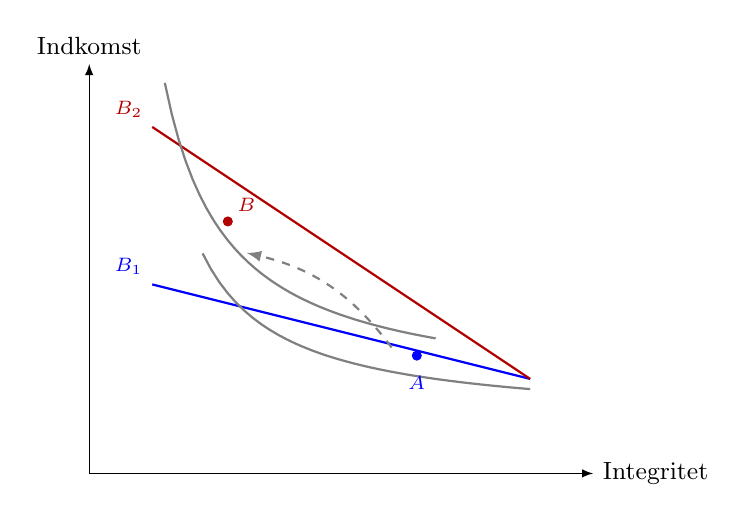
\begin{tikzpicture}[>=latex, scale=0.8, every node/.style={font=\small}]
  \draw[->] (0,0) -- (8,0) node[right] {Integritet};
  \draw[->] (0,0) -- (0,6.5) node[above] {Indkomst};
  % B1 moderat
  \draw[thick, blue] (1.0,3.0) -- (7.0,1.5);
  \node[blue, above left, font=\scriptsize] at (1.0,3.0) {$B_1$};
  % B2 aggressiv
  \draw[thick, red!70!black] (1.0,5.5) -- (7.0,1.5);
  \node[red!70!black, above left, font=\scriptsize] at (1.0,5.5) {$B_2$};
  % Indifferenskurver
  \draw[thick, gray, domain=1.8:7.0, samples=40]
    plot (\x, {3.5/(\x-0.5) + 0.8});
  \draw[thick, gray, domain=1.2:5.5, samples=40]
    plot (\x, {5.0/(\x-0.2) + 1.2});
  % Punkt A
  \filldraw[blue] (5.2,1.87) circle (2pt);
  \node[below, blue, font=\bfseries\scriptsize] at (5.2,1.7) {$A$};
  % Punkt B
  \filldraw[red!70!black] (2.2,4.0) circle (2pt);
  \node[above right, red!70!black, font=\bfseries\scriptsize] at (2.2,4.0) {$B$};
  \draw[->, thick, dashed, gray] (4.8,2.0) to[bend right=20] (2.5,3.5);
\end{tikzpicture}
\caption{\textbf{Integrity vs.\ Income.} $B_1$ (moderat insentiv): optimum $A$ med høy integritet. $B_2$ (aggressivt insentiv): optimum $B$ med lav integritet, høy inntekt. Kompensasjonsdesignet endrer atferd uten å endre preferanser. [SLIDE -- BSZ kap.\ 2]}
\end{figure}

\subsection*{Grafisk modell 2 -- Risk vs.\ Expected Value}

\begin{figure}[h]
\centering
\begin{tikzpicture}[>=latex, scale=0.8, every node/.style={font=\small}]
  \draw[->] (0,0) -- (8,0) node[right] {$\sigma_W$ (risiko)};
  \draw[->] (0,0) -- (0,7) node[above] {$E[W]$};
  % Risikoavers
  \draw[thick, blue, domain=0:5.5, samples=40]
    plot (\x, {1.5 + 0.15*\x*\x});
  \node[blue, right, font=\scriptsize] at (5.5,6.0) {risikoavers ($r>0$)};
  \draw[thick, blue, dashed, domain=0:4.5, samples=40]
    plot (\x, {2.5 + 0.15*\x*\x});
  % Risikonøytral
  \draw[thick, green!50!black] (0,3.0) -- (7.0,3.0);
  \node[green!50!black, right, font=\scriptsize] at (7.0,3.0) {risikonøytral ($r=0$)};
  % CE og RP
  \node[left, font=\scriptsize] at (0,1.5) {$CE$};
  \filldraw[blue] (3.5,3.34) circle (1.5pt);
  \node[above left, font=\bfseries\scriptsize, blue] at (3.5,3.34) {$A$};
  \draw[dashed] (3.5,0) -- (3.5,3.34);
  \draw[dashed] (0,3.34) -- (3.5,3.34);
  \node[left, font=\scriptsize] at (0,3.34) {$E[W]_A$};
  \draw[decorate, decoration={brace, amplitude=4pt, mirror}, red!70!black] (-0.3,1.5) -- (-0.3,3.34);
  \node[left, font=\scriptsize, red!70!black] at (-0.6,2.42) {$RP$};
  \node[below, font=\scriptsize] at (3.5,0) {$\sigma_A$};
\end{tikzpicture}
\caption{\textbf{Risk--Expected Value.} Risikoavers agent (blå): stigende, konvekse indifferenskurver. $CE$ = certainty equivalent (skjæring $y$-akse). $RP = E[W]_A - CE = \tfrac{r}{2}\beta^2\sigma^2$. Risikonøytral (grønn): flat -- ingen risikopremie. [SLIDE -- BSZ kap.\ 2/15]}
\end{figure}

\subsection*{Real-world eksempler}

\textbf{Eks.~1 -- Wells Fargo (2016) -- integrity vs.\ income i praksis.}\quad [EKS]
Wells Fargos aggressive cross-sell-kvoter (høy $\beta$ på antall solgte produkter) roterte budsjettlinjen i integrity-income-rommet. Ansatte valgte punkt $B$: 3{,}5 mill.\ falske kontoer åpnet. Etter skandalen (\$185M bot, CEO trådte av) ble $\beta$ redusert og kvalitative mål innført -- budsjettlinjen rotert tilbake mot integritet. Modell 1 forklarer mekanismen presist: det var systemet, ikke personene, som var feil.

\textbf{Eks.~2 -- Equinor-ansatte og aksjespareprogram, sammenligning.}\quad [EKS]
Equinor tilbyr aksjeprogram med rabatt: ansatte velger frivillig mellom lav-risiko (fastlønn, 100\%) og høy-risiko (fastlønn + aksjer, usikkert). Konservative ingeniører med høy boliggjeld velger lite eksponering (bratte indifferenskurver, høy $r$). Risikotolerante seniorledere velger mer aksjer (flate kurver, lav $r$). Modell 2 forklarer seleksjonsmønsteret. Sammenligningen med Wells Fargo: begge handler om kompensasjonsdesignets effekt på atferd -- Wells Fargo om etisk dimensjon (modell 1), Equinor om risiko-dimensjon (modell 2). Samme nytteteori, to ulike godsrom.

\subsection*{Kobling til Mærsk Power-to-X}
\textbf{Modell 1:} PtX-prosjektledere kan fristes til å oppblåse prognoser og underkommunisere risiko hvis bonusen er knyttet til prosjektgodkjenning -- budsjettlinjen premierer ``lav integritet'' (overoptimistiske estimater). Løsning: claw-back-klausuler og subjektiv evaluering som bevarer integritet-insentiv. \textbf{Modell 2:} PtX har svært stor $\sigma$ (teknologirisiko, reguleringsrisiko, markedsrisiko). Risikoaverse ledere krever høy $E[W]$ for å akseptere stillingen -- synlig i PtX-divisjonens lønnsstruktur: høy grunnlønn + moderat $\beta$ på milestones (jf.\ \thref{informativeness-principle}{informativeness}). [CASE]

\subsection*{Fallgruber}
\begin{itemize}\setlength{\itemsep}{2pt}
\item Bare beskrive én modell -- spørsmålet ber om \emph{begge}.
\item Tegne indifferenskurvene feil: modell 1 = konvekse mot origo (standard), modell 2 = konvekse \emph{oppover} (stigende i risiko).
\item Forveksle certainty equivalent med reservation utility -- CE er nyttemessig ekvivalent beløp; reservation utility er minimumsnytte for deltagelse.
\item Glemme risikopremie-formelen $RP = \tfrac{r}{2}\beta^2\sigma^2$.
\item Ikke koble modellene til hverandre via $\beta$ -- begge handler om konsekvenser av kontraktsdesign.
\item Glemme at modell 1 viser atferdsendring \emph{uten preferanseendring} -- det er budsjettlinjen, ikke indifferenskurvene, som endres.
\end{itemize}

\subsection*{Håndskrivbar disposisjon (15-min forberedelse)}
\begin{itemize}\setlength{\itemsep}{2pt}
\item \textbf{Tese:} To nyttemodeller: (1) integritet vs.\ indkomst -- kompensasjonsdesign påvirker etisk atferd; (2) risiko vs.\ forventet verdi -- risikoaversjon bestemmer risikopremie.
\item \textbf{Modell 1:} Akser: integritet (x), indkomst (y). Indifferenskurver konvekse. Budsjettlinje = kompensasjonsplan. Aggressivt insentiv $\Rightarrow$ rotasjon $\Rightarrow$ punkt $A\to B$. Tegn!
\item Nøkkelinnsikt: system, ikke person. $\beta$ driver rotasjonen.
\item \textbf{Modell 2:} Akser: $\sigma_W$ (x), $E[W]$ (y). Indifferenskurver: $E[W] = \bar{U} + \tfrac{r}{2}\sigma^2$. Risikoavers: stigende, konveks. Risikonøytral: flat. Tegn!
\item $CE$, $RP = \tfrac{r}{2}\beta^2\sigma^2$, reservation utility.
\item \textbf{Kobling:} $\beta$ er den felles designvariabelen. Høy $\beta$ $\Rightarrow$ (1) mer fristelse, (2) mer risiko.
\item Eks.\ 1: Wells Fargo 2016 (modell 1 -- falske kontoer). Eks.\ 2: Equinor aksjeprogram (modell 2 -- valg av risiko).
\item Case: Mærsk PtX -- prognoseinflasjon (mod.\ 1) + lederrekruttering med høy $\sigma$ (mod.\ 2).
\item Søyle: \SThree\ (kompensasjonsdesign) + \STwo\ (hva som måles driver atferd).
\end{itemize}


\part{Teorier (utdypende)}
% !TEX root = ../main.tex
\section{Responsibility Centers -- de 5 centertyper}\label{thr:responsibility-centers}

\paragraph{Definisjon.} Et \emph{responsibility center} er en organisatorisk enhet (avdeling, divisjon, datterselskap) som lederen holdes ansvarlig for via et avgrenset sett av regnskapsmessige måltall. Centertypen bestemmer både hvilke beslutningsrettigheter lederen får (S1) og hvilke prestasjoner som måles og belønnes (S2/S3). BSZ kap. 17 deler virksomhetens enheter i fem typer: \textbf{cost center}, \textbf{expense center}, \textbf{revenue center}, \textbf{profit center} og \textbf{investment center}. [SLIDE]

\subsection*{Forklaring}

Når en virksomhet desentraliserer beslutninger til divisjonsledere, må toppledelsen velge \emph{hvilke variabler lederen kan styre} og \emph{hvordan resultatet skal måles}. Valget av centertype er et samtidig design av (i) beslutningsrettigheter (input-mix, pris, volum, investering), (ii) regnskapsmessig prestasjonsmål (kostnad, omsetning, profit, ROA/EVA) og (iii) belønningsstruktur. Dette er kjernen i det BSZ kaller \emph{organizational architecture}: de tre dimensjonene må passe sammen. [SLIDE/BOK]

Det grunnleggende prinsippet bak inndelingen er \thref{controllability-principle}{Controllability-prinsippet}: en leder bør bare evalueres på utfall hun faktisk kan kontrollere. Hvis en leder ikke har beslutningsmyndighet over for eksempel salgspris, gir det ikke mening å holde henne ansvarlig for omsetning. Sentertypene reflekterer derfor ulik bredde i delegert beslutningsrett. [SLIDE]

\begin{center}
\begin{tabular}{@{}p{2.6cm}p{4.0cm}p{4.0cm}p{3.0cm}@{}}
\toprule
\textbf{Centertype} & \textbf{Lederen kontrollerer} & \textbf{Måles på} & \textbf{Typiske enheter} \\
\midrule
Cost center & Input-mix, produksjonsmetode (gitt output) & Kostnad pr.\ enhet, total kostnad, output pr.\ budsjettkrone & Produksjon, sykehus, jernbane \\
Expense center & Aktivitetsnivå innenfor budsjett & Forbruk vs.\ budsjett (output er vanskelig å måle objektivt) & HR, regnskap, PR, R\&D \\
Revenue center & Salgsmix, salgsinnsats (priser ofte sentralt fastsatt) & Salgsinntekt vs.\ budsjett & Salgsavdelinger, distribusjon \\
Profit center & Input-mix, produktmiks, salgspris & Profit (omsetning $-$ kostnad) & Forretningsdivisjoner med eget P\&L \\
Investment center & Profitcenter + kapitalinvesteringer & ROA, IRR, EVA & Datterselskaper, store divisjoner \\
\bottomrule
\end{tabular}
\end{center}

\subsubsection*{1. Cost center}
Enheten har ansvar for å minimere kostnader gitt et utfallskrav, eller å maksimere output gitt et budsjett. Lederen styrer kombinasjonen av innsatsfaktorer og produksjonsmetode, men har ikke ansvar for omsetning eller pris. Typiske eksempler: produksjonsavdelinger, sykehus, jernbanedrift. [SLIDE]

\emph{Sentralt poeng:} Minimering av gjennomsnittskostnad gir \textbf{ikke} nødvendigvis profitmaksimering -- kostnadsfokus alene kan gi for lav kvalitet eller feil produktmiks. Dette er en gjentakende kritikk av kostnadsstyring i isolasjon. [SLIDE]

\subsubsection*{2. Expense center}
En spesialform av cost center brukt der \emph{output er vanskelig å kvantifisere objektivt}. Lederen får et fast budsjett og evalueres på om aktivitetene leveres innenfor budsjettet, ofte subjektivt. Typiske eksempler: HR, regnskap, PR, R\&D, juridisk avdeling. [SLIDE]

\emph{Sentralt problem:} Når output ikke kan måles, oppstår fare for \emph{empire building} (lederen vil ha større budsjett enn nødvendig), \emph{overconsumption} (penger brukes opp fordi de er der), og generelt vansker med å avgjøre om enheten er produktiv. [SLIDE]

\subsubsection*{3. Revenue center}
Enheten har ansvar for å maksimere omsetning innenfor et gitt budsjett. Lederen styrer salgsinnsats og produktmiks, mens priser og ofte produktportefølje fastsettes sentralt. Typiske eksempler: salgsdivisjoner, distribusjonsavdelinger. [SLIDE]

\emph{Sentralt problem:} Omsetningsmaksimering ($MR = 0$) er ikke det samme som profitmaksimering ($MR = MC$). Et rent revenue center kan derfor presse pris/volum i retninger som er gode for omsetningen, men ikke for selskapets samlede profit -- særlig hvis selgere kan tilby store rabatter eller dyre kundeløsninger. [SLIDE]

\subsubsection*{4. Profit center}
Enheten har ansvar for både kostnader og inntekter. Lederen styrer input-mix, produktmiks og salgspris, og evalueres på regnskapsmessig profit. Typiske eksempler: forretningsdivisjoner med eget resultatregnskap (f.eks.\ en bilprodusents merkevaredivisjon). [SLIDE]

\emph{Forutsetning for at det fungerer:} Lederen må ha \emph{spesifik viden} (lokal kunnskap) som det ville være kostbart å sende oppover, samtidig som divisjonens beslutninger primært påvirker dens egen profit. Når disse forutsetningene brytes, kommer divisjonene i konflikt: \emph{eksternaliteter} mellom divisjoner, \emph{free-riding} på felles merkenavn, og \emph{transfer pricing-konflikter} ved interne leveranser. [SLIDE/BOK]

\subsubsection*{5. Investment center}
Et profitcenter som i tillegg har myndighet over kapitalinvesteringer. Lederen evalueres på avkastning på den investerte kapitalen -- typisk \emph{Return on Assets} (ROA = regnskapsmessig nettoresultat / total kapital i senteret), \emph{IRR}, eller \emph{Economic Value Added} (EVA = NOPAT $-$ WACC $\times$ kapital). [SLIDE]

\emph{Sentralt problem:} Kortsiktige regnskapsmål kan avskrekke gode langsiktige investeringer. Et investment center evaluert kun på årlig ROA kan utsette eller avvise prosjekter med positiv NPV fordi avskrivninger og oppstartskostnader drar ROA ned første år. EVA forsøker å rette dette ved å trekke fra kapitalkostnaden direkte. [SLIDE/BOK]

\subsection*{Kjerneforutsetninger}
\begin{itemize}
\item \textbf{Controllability:} Lederen må faktisk kunne styre de variablene hun evalueres på. Brutt forutsetning $\Rightarrow$ urettferdig og demotiverende.
\item \textbf{Målbarhet:} Det resultatmålet centertypen bygger på må kunne måles tilstrekkelig presist (kostnad, omsetning, profit, kapitalavkastning).
\item \textbf{Spesifik vs.\ generell viden (Jensen \& Meckling):} Desentralisering (profit-/investmentcenter) er attraktivt når lokal kunnskap er kostbar å overføre. Når kunnskapen er sentralt tilgjengelig, peker det mot cost-/expense-center.
\item \textbf{Lav grad av eksternaliteter mellom enheter:} Jo mer divisjonene påvirker hverandre (felles kunder, felles ressurser, interne leveranser), desto mindre egnet er rene profit-/investmentcentre uten transfer pricing-regime.
\item \textbf{Stabilt mål-måleforhold:} Måltallet må gjenspeile reell verdiskaping. Brutt forutsetning gir \emph{gaming} (jf.\ ratchet, horisontproblem).
\end{itemize}

\subsection*{Muligheter (når hver type bør velges)}
\begin{itemize}
\item \textbf{Cost center} -- velges når enheten leverer et standardisert output som er lett å måle, men ikke har ansvar for pris eller marked. Produksjonshaller, IT-drift, lagerterminaler.
\item \textbf{Expense center} -- velges når output er vanskelig å kvantifisere og enheten leverer støtte/innsats snarere enn et målbart produkt. R\&D, HR, regnskap, PR. Budsjettstyring + subjektiv vurdering er det realistiske alternativet.
\item \textbf{Revenue center} -- velges når enheten har innflytelse på salg og kundekontakt, men ikke skal bestemme pris eller produktmiks. Vanlig der toppledelsen vil holde priskontrollen sentralt (merkebeskyttelse, prisdiskriminering).
\item \textbf{Profit center} -- velges når lederen sitter på spesifik lokal viden om både kostnader og marked, og divisjonen kan operere relativt selvstendig. Geografiske divisjoner, produktdivisjoner.
\item \textbf{Investment center} -- velges når også investeringsbeslutninger krever lokal kunnskap (markedsspesifikke prosjekter, ny kapasitet) og enheten er stor nok til at avkastning på kapital kan måles meningsfullt.
\end{itemize}

\subsection*{Begrensninger og kritikk}
\begin{itemize}
\item \textbf{Cost center:} Risiko for at kvalitet, leveringspresisjon og innovasjon ofres for å minimere målte kostnader. Lederen kan velte kostnader over på andre enheter (urealistiske internprisingseffekter).
\item \textbf{Expense center:} Output-måling er subjektiv $\Rightarrow$ rom for politisk spill, empire building og \emph{soft budget constraints}. Vanskelig å avgjøre om enheten er for stor.
\item \textbf{Revenue center:} Maksimering av omsetning $\neq$ profit. Selgere kan gi for store rabatter eller selge til dårlige kunder for å nå omsetningsmål. Trenger ofte komplementære marginmål.
\item \textbf{Profit center:} Skaper interne eksternaliteter (én divisjons valg påvirker en annens profit), \emph{free-riding} på fellesgoder (merkevare, FoU), og strid om internpriser. Risiko for at lokal profit slår fellesnyttig samarbeid i hjel.
\item \textbf{Investment center:} ROA og lignende regnskapsmål er korttidsforvridde -- avskrivninger og engangskostnader straffer langsiktige investeringer. ROA kan også manipuleres ved å selge unna aktiva (\emph{asset stripping}). EVA hjelper, men krever korrekt kapitalkostnad.
\item \textbf{Generelt:} Alle målbaserte centertyper er sårbare for \emph{gaming}, \emph{horisontproblem} og \emph{ratchet-effekt}. Centertypen alene løser ikke insentivproblemet -- den må kombineres med riktig kontraktsdesign (jf.\ informativeness-principle).
\end{itemize}

\subsection*{Modell / oversikt}

Centertypene kan ordnes i en \emph{stige av delegert beslutningsrett}: jo flere kontrollvariabler lederen får, desto bredere måltall trenger evalueringen.

\begin{center}
\begin{tabular}{@{}lcccc@{}}
\toprule
 & \textbf{Kostnader} & \textbf{Inntekter} & \textbf{Profit} & \textbf{Kapital} \\
\midrule
Cost center & \checkmark & & & \\
Expense center & (budsjett) & & & \\
Revenue center & & \checkmark & & \\
Profit center & \checkmark & \checkmark & \checkmark & \\
Investment center & \checkmark & \checkmark & \checkmark & \checkmark \\
\bottomrule
\end{tabular}
\end{center}

\textit{Tabellen viser hvilke størrelser lederen i hver centertype har beslutningsrett og resultatansvar for. [SLIDE -- BSZ kap.\ 17, slide 4]}

\subsection*{Eksempler}
\begin{itemize}
\item \textbf{Equinor (NO):} Letevirksomheten på norsk sokkel kjøres som et \emph{investment center} -- lederne bestemmer letebrønner og felt\-utbygginger og måles på avkastning på investert kapital. Raffinerivirksomheten Mongstad har historisk vært drevet mer som et \emph{cost center}, der lederen styrer effektivitet i prosessen, mens markedspriser settes globalt. [EKS]
\item \textbf{IKEA:} Den enkelte varehussjef driver et \emph{profit center} -- styrer lokal bemanning, kampanjer og produktutvalg innenfor konsernkonsept, og måles på resultatbidrag. Sentralfunksjoner som design (Älmhult) og IT er \emph{expense centers} på fast budsjett. [EKS]
\item \textbf{Maersk:} Shipping-divisjonene Ocean og Logistics \& Services drives som separate profit/investment centers med egne P\&L og kapitalbudsjetter, mens IT- og HR-funksjoner i konsernet er expense centers. [EKS/CASE]
\item \textbf{NSB/Vy (jernbanedrift):} Togdrift har lenge vært et klassisk \emph{cost center} -- billetter og ruter er regulert, så lederne måles på driftskostnad pr.\ togkilometer. Da Vy-konsernet ble organisert i forretningsenheter, ble enkelte selskaper omgjort til profit centers, noe som økte fokuset på kommersielle ruter og endret atferd merkbart. [EKS]
\item \textbf{Salgsdivisjoner i farmasi (f.eks.\ Novo Nordisk):} Lokale salgsteam er gjerne \emph{revenue centers} fordi priser forhandles sentralt og refusjonssystemer er stabile -- men kombineres med marginvilkår for å unngå at selgere skyver lavmargin-produkter. [EKS]
\end{itemize}

\subsection*{Kobling til søyle og andre teorier}
Søyle: \STwo\ (centertypen \emph{er} et prestasjonsmålingsregime), men også \SOne\ (allokering av beslutningsrett) og \SThree\ (måltallet kobles til belønning). Centertyper er derfor et godt eksempel på at de tre søylene må designes samlet.

Relaterte teorier: \thref{controllability-principle}{Controllability-prinsippet} (grunnregelen bak valget), \thref{transfer-pricing}{Transfer pricing} (oppstår nettopp når man har profit-/investmentcentre med interne leveranser), \thref{decision-management-control}{Decision Management vs.\ Decision Control} (centertyper definerer hvem som initierer/implementerer vs.\ ratifiserer/monitorerer), \thref{specific-vs-general-knowledge}{Spesifik vs.\ generell viden} (Jensen \& Meckling-argumentet for når desentralisering lønner seg), \thref{ratchet-effect}{Ratchet-effekten} (gaming-problem som rammer alle målbaserte centre).

\paragraph{Brukt i spørsmål:} Q01, Q02, Q05.

% !TEX root = ../main.tex
\section{Controllability-prinsippet}\label{thr:controllability-principle}

\paragraph{Definisjon.} Controllability-prinsippet sier at en leder kun skal evalueres og belønnes på utfall hun selv kan kontrollere. Utfall som er drevet av faktorer utenfor lederens beslutningsrom (eksogene markedssvingninger, andre divisjoners adferd, makroforhold) skal filtreres bort fra prestasjonsmålet. [SLIDE]

\subsection*{Forklaring}

Prinsippet er et normativt rettferdighets- og effektivitetskrav: hvis lederen straffes eller belønnes for variasjon hun ikke har innvirkning på, blir signalet i prestasjonsmålet støyete og insentivene svekkes. Risikoaverse ledere må også kompenseres med høyere lønn for å bære ikke-kontrollerbar risiko (jf.\ \thref{informativeness-principle}{informativeness-principle}), noe som gjør slike kontrakter dyre for prinsipalen. Prinsippet ligger bak hele inndelingen i \thref{responsibility-centers}{responsibility centers} -- man skreddersyr måltallet til lederens faktiske kontrollvariabler. [SLIDE/BOK]

I praksis er ikke skillet mellom kontrollerbart og ikke-kontrollerbart skarpt. En divisjonsleder kontrollerer ikke valutakurser direkte, men kan velge å sikre seg mot dem. En produksjonssjef kontrollerer ikke råvarepriser, men kan velge leverandører. Anvendelse av prinsippet krever derfor en konkret vurdering av \emph{hvilken type} kontroll lederen reelt har. [BOK]

\subsection*{Kjerneforutsetninger}
\begin{itemize}
\item Det er mulig å skille kontrollerbare fra ikke-kontrollerbare faktorer i målingen (regnskapsmessig eller analytisk).
\item Lederen er risikoaversiv -- ellers ville hun gjerne tatt på seg ukontrollerbar risiko gratis.
\item Informasjonen om hva som er kontrollerbart er rimelig symmetrisk; ellers oppstår diskusjon om hva som egentlig var ``utenfor lederens kontroll''.
\end{itemize}

\subsection*{Muligheter}
\begin{itemize}
\item Gir grunnlag for å velge \emph{riktig centertype} ut fra lederens beslutningsrettigheter.
\item Reduserer kompensasjon for risiko -- billigere insentivkontrakter.
\item Reduserer demotivering: ledere som ``rammes'' av ukontrollerbare svingninger gir opp innsats (locus of control-effekt).
\item Begrunner bruk av \emph{relative performance evaluation} (sammenligning mot peers) for å filtrere ut bransje-/makrostøy.
\end{itemize}

\subsection*{Begrensninger og kritikk}
\begin{itemize}
\item Strikt anvendelse kan fjerne all risikodeling -- men noen ganger \emph{ønsker} prinsipalen at lederen bærer risiko (eierperspektiv, langsiktig hensyn).
\item Mange utfall er delvis kontrollerbare. Hvor settes grensen?
\item Lederen kan strategisk omklassifisere dårlige resultater som ``ikke-kontrollerbart'' (\emph{ex-post excuse}) og gode som ``mitt verk''.
\item Prinsippet sier ikke noe om hvilket \emph{nivå} av målet som er riktig (gaming, ratchet-problemer ligger fortsatt der).
\item I virkeligheten ønsker eier ofte at ledere tar ansvar utover egen kontroll -- f.eks.\ CEO som påvirker selskapets evne til å håndtere kriser de ikke skapte selv.
\end{itemize}

\subsection*{Modell / illustrasjon}

\begin{figure}[H]
\centering
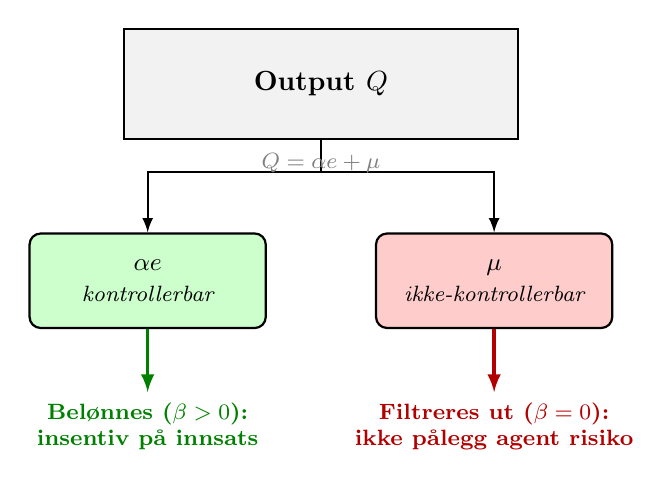
\begin{tikzpicture}[>=latex, every node/.style={font=\small}]
  % Output Q (stor boks)
  \node[draw, thick, fill=gray!10, minimum width=5.0cm, minimum height=1.4cm, font=\bfseries] (Q) at (0,3) {Output $Q$};
  % Dekomponering: alpha*e + mu
  \node[draw, rounded corners, thick, fill=green!20, minimum width=3.0cm, minimum height=1.2cm, align=center] (E) at (-2.2,0.5) {$\alpha e$\\ \footnotesize\itshape kontrollerbar};
  \node[draw, rounded corners, thick, fill=red!20, minimum width=3.0cm, minimum height=1.2cm, align=center] (M) at (2.2,0.5) {$\mu$\\ \footnotesize\itshape ikke-kontrollerbar};
  % Piler fra Q til dekomp
  \draw[->, thick] (Q.south) -- ++(0,-0.4) -| (E.north);
  \draw[->, thick] (Q.south) -- ++(0,-0.4) -| (M.north);
  \node[font=\footnotesize, gray] at (0,2.0) {$Q = \alpha e + \mu$};
  % Pil ned til β-beslutning
  \draw[->, very thick, green!50!black] (E.south) -- ++(0,-0.8)
    node[below, font=\footnotesize\bfseries, align=center] {Belønnes ($\beta > 0$):\\ insentiv på innsats};
  \draw[->, very thick, red!70!black] (M.south) -- ++(0,-0.8)
    node[below, font=\footnotesize\bfseries, align=center] {Filtreres ut ($\beta = 0$):\\ ikke pålegg agent risiko};
\end{tikzpicture}
\caption{\textbf{Controllability-prinsippet.} Mål agenten på den delen av $Q$ hun \emph{kontrollerer} ($\alpha e$), og filtrer bort det hun \emph{ikke} kontrollerer ($\mu$ -- markedssjokk, valuta, peer-firmaer). I praksis: bruk relative måltall, ekskluder ekstraordinære poster, eller dekomponer KPI-er. Strikt anvendelse senker risikopremien uten å svekke insentivet. [SLIDE -- BSZ kap.\ 10]}
\end{figure}

I prinsipal-agent-modellen $W = W_0 + \beta Q$ er $Q$ et målt prestasjonstall. Controllability-prinsippet sier at vekten $\beta$ bør være null på komponenter i $Q$ som lederen ikke kontrollerer, og positiv kun på komponenter hun \emph{kan} påvirke. Tilsvarende: når støyen i $Q$ øker, må $W_0$ (fast lønn) opp og $\beta$ ned (informativeness-prinsippet).

\begin{center}
\begin{tabular}{@{}lll@{}}
\toprule
\textbf{Kontroll lederen har} & \textbf{Egnet centertype} & \textbf{Måltall} \\
\midrule
Kun input-mix (output gitt) & Cost center & Kostnad pr.\ enhet \\
Kun aktivitetsnivå & Expense center & Budsjettoverholdelse \\
Salgsinnsats, kundekontakt & Revenue center & Omsetning \\
Pris, mix, kostnad & Profit center & Profit \\
Profit + investeringer & Investment center & ROA, EVA \\
\bottomrule
\end{tabular}
\end{center}

\subsection*{Eksempler}
\begin{itemize}
\item \textbf{SAS:} Flight crew kan ikke holdes ansvarlig for drivstoffpris-svingninger. Crew evalueres på punktlighet og kundeservice (kontrollerbart), ikke drivstoffmargin (ikke-kontrollerbart). [EKS]
\item \textbf{Equinor:} Lete-avdelingen evalueres på funnrate og kostnad pr.\ funn, ikke på oljeprisen, fordi prisen er global og eksogen. [EKS]
\item \textbf{Norsk Hydro:} Aluminium-divisjonene har historisk hatt resultatregnskap justert for aluminiumspris (LME-pris) for å isolere driftsbidraget fra prissyklusen. [EKS]
\end{itemize}

\subsection*{Kobling til søyle og andre teorier}
Søyle: \STwo\ primært, men direkte koblet til \SThree\ (kompensasjon) og \SOne\ (beslutningsrett $=$ det som er kontrollerbart). Relatert: \thref{responsibility-centers}{Responsibility centers}, \thref{informativeness-principle}{Informativeness-prinsippet}, \thref{absolute-vs-relative-performance}{Relative performance evaluation}.

\paragraph{Brukt i spørsmål:} Q01, Q05, Q10, Q14.

% !TEX root = ../main.tex
\section{Transfer Pricing -- interne afregningspriser}\label{thr:transfer-pricing}

\paragraph{Definisjon.} \emph{Transfer pricing} er den prisen som settes når en divisjon i et konsern leverer en vare eller tjeneste internt til en annen divisjon. Prisen påvirker både den enkelte divisjonens regnskapsmessige profit (S2), insentivene til divisjonslederne (S3) og hvilke produksjons- og investeringsbeslutninger som faktisk treffes (S1). Den teoretisk korrekte transfer prisen er lik selgerdivisjonens \emph{opportunity cost} (offeromkostning) ved den interne leveransen. [SLIDE]

\subsection*{Forklaring}

Transfer pricing oppstår nødvendigvis når et konsern desentraliserer ansvar i \thref{responsibility-centers}{profit- eller investmentcentre} med interne leveranser. Hver divisjon har sitt eget P\&L; samme transaksjon må derfor prises som inntekt for selger og kostnad for kjøper. Valget av prismetode bestemmer både \emph{fordelingen} av profit mellom divisjonene og \emph{nivået} av intern handel -- og dermed hvor effektivt konsernet utnytter sine egne ressurser. [SLIDE/BOK]

Pensum skiller mellom to informasjonsregimer som gir vidt forskjellige konklusjoner:

\paragraph{(a) Costless information (symmetrisk, full informasjon).} Toppledelsen kjenner alle marginalkostnader, kapasiteter og opportunity cost-funksjoner. Førstebestes-løsningen er å sette transfer prisen lik selgerdivisjonens \emph{marginal opportunity cost}: hvis det er ledig kapasitet er dette marginalkostnaden ($MC$); hvis kapasiteten er bundet, er det marginalkostnaden \emph{pluss} dekningsbidraget på den fortrengte eksterne salgsenheten. Dette gir konsernoptimal mengde, fordi kjøperdivisjonen utvider intern handel akkurat så lenge dens marginale betalingsvilje overstiger den reelle alternativkostnaden. Resultatet er ekvivalent med MR=MC for konsernet samlet. [SLIDE]

\paragraph{(b) Asymmetrisk informasjon.} I praksis sitter divisjonslederne på \emph{spesifik viden} (jf.\ \thref{specific-vs-general-knowledge}{spesifik vs.\ generell viden}) om egne kostnader, kapasitet og marked. Toppledelsen kan ikke verifisere kostnadsdata uten kostnad. Dette skaper to problemer som rammer alle prisingsmetoder: (i) selgerdivisjonen har insentiv til å \emph{overrapportere} kostnader for å presse opp transfer prisen og dermed sin egen profit; (ii) kjøperdivisjonen kan tilsvarende overdrive interne alternativer for å presse prisen ned. Dette er et klassisk \thref{principal-agent}{prinsipal-agent}-problem på tvers av interne grenser, og det er grunnen til at ingen enkelt metode er optimal. Trade-off-en mellom \emph{decision management} (riktig pris for riktig beslutning) og \emph{decision control} (riktig insentiv for lederen) blir tydelig: presise tall er ikke nødvendigvis insentivkompatible. [SLIDE/BOK]

\subsection*{De fem metodene i pensum}

\paragraph{1. Market-based transfer pricing.} Bruker eksterne markedspriser når det finnes et konkurransedyktig marked for varen. Når markedet er fullkomment, sammenfaller markedspris og opportunity cost, og denne metoden gir både konsernoptimal beslutning og rettferdige insentiver. Krever et reelt og likvid eksternt marked. [SLIDE]

\paragraph{2. Marginal cost (MC) pricing.} Transfer pris $=$ selgerens marginalkostnad. Gir konsernoptimale beslutninger \emph{når kapasiteten er ledig} (opportunity cost $=$ MC). Problem: dekker ikke faste kostnader, så selgerdivisjonen taper penger på interne salg og demotiveres -- og lederen får insentiv til å overrapportere MC. [SLIDE]

\paragraph{3. Full cost pricing.} Transfer pris $=$ MC $+$ allokerte faste kostnader. Enkel å beregne, vanlig i praksis. Problemet er at full cost typisk \emph{overstiger} opportunity cost, slik at intern mengde blir for lav (kjøperen vrir seg mot eksterne leverandører selv når det er suboptimalt for konsernet) -- en intern \thref{double-markup}{double markup}-effekt. [SLIDE]

\paragraph{4. Full cost plus markup (cost-plus).} Full cost $+$ et avtalt prispåslag. Gir selger et garantert dekningsbidrag og dermed bedre insentiver. Forsterker likevel double-markup-problemet og gir lederne enda sterkere insentiv til å skjule reell MC. [SLIDE/BOK]

\paragraph{5. Negotiated transfer pricing.} Divisjonene forhandler prisen seg imellom. Kan ende nær opportunity cost \emph{når begge har omtrent like sterk forhandlingsposisjon}. Resultatet avhenger av forhandlingsevner, ikke av økonomi; tidkrevende; risiko for stadige konflikter som må eskaleres til toppledelsen. [SLIDE]

\paragraph{(Bonus) Dual pricing.} Selger krediteres til markedspris (eller MC $+$ markup), mens kjøper debiteres til marginal cost. Konsernregnskapet rettes så opp internt. Løser insentivproblemet på papiret, men er kostbart, gjør resultatregnskapene mindre transparente og åpner for spill. [BOK]

\subsection*{Kjerneforutsetninger}
\begin{itemize}
\item \textbf{Desentralisering:} Konsernet har minst to enheter med egne P\&L (typisk profit- eller investmentcentre).
\item \textbf{Intern handel:} Det finnes et faktisk varestrøms- eller tjenesteflyt mellom enhetene.
\item \textbf{Målbarhet av kostnad og inntekt:} Kostnader skal kunne henføres til den interne transaksjonen.
\item \textbf{Antakelse om informasjonsregime:} Costless information (a) gir én anbefaling (opportunity cost-pris); asymmetrisk informasjon (b) krever andrebestes-løsninger.
\item \textbf{Eksternt marked (kun market-based):} Det må finnes et likvid og konkurransedyktig eksternt marked for samme vare.
\item \textbf{Kapasitetsforutsetning:} MC-pricing forutsetter ledig kapasitet; ved kapasitetsbinding må prisen heves med opportunity cost av fortrengt eksternt salg.
\end{itemize}

\subsection*{Muligheter}
\begin{itemize}
\item Lar konsernet beholde fordelene ved desentralisering (lokal kunnskap, motivasjon, klare resultatansvar) og samtidig styre intern ressursbruk.
\item Gjør intern verdiskaping synlig i regnskapet og legger grunnlag for divisjonell prestasjonsmåling.
\item Eksponerer interne ineffektiviteter (en divisjon som ikke er konkurransedyktig mot markedet blir tydelig).
\item Brukes også i skatte\-optimalisering (multinasjonale konserner allokerer profit til lavskatteland) -- men dette er regulert av OECDs armlengde-prinsipp.
\end{itemize}

\subsection*{Begrensninger og kritikk}
\begin{itemize}
\item \textbf{Ingen metode er førstebeste under asymmetrisk informasjon.} Alle gir trade-off mellom riktig beslutning og riktig insentiv (decision management vs.\ decision control).
\item \textbf{Gaming og manipulasjon:} Lederne har insentiv til å rapportere kostnader strategisk -- både for å øke egen profit og for å påvirke fremtidige forhandlinger (\emph{ratchet}-lignende effekt).
\item \textbf{Interne konflikter:} Transfer pricing-strider er en av de hyppigste kildene til organisatorisk friksjon i divisjonsstrukturer; eskaleres ofte til toppledelsen.
\item \textbf{Double markup:} Når både selger og kjøper legger på et eget margin, blir samlet pris høyere enn samfunnsoptimal -- intern mengde og samlet profit reduseres.
\item \textbf{Markedspriser kan mangle:} For halvfabrikater og spesialiserte tjenester finnes ofte ikke noe likvid eksternt marked.
\item \textbf{Kapasitetsendringer:} Riktig opportunity cost endres med kapasitetsutnyttelsen, så ``riktig'' transfer pris bør i prinsippet variere over tid -- noe få selskaper får til.
\item \textbf{Skatte- og reguleringsrisiko:} Aggressiv intern prising kan utløse skattetvister (jf.\ armlengdeprinsippet, BEPS).
\end{itemize}

\subsection*{Modell / oversikt}

\begin{center}
\renewcommand{\arraystretch}{1.2}
\begin{tabular}{@{}p{3.4cm}p{4.6cm}p{4.6cm}p{2.0cm}@{}}
\toprule
\textbf{Metode} & \textbf{Fordele} & \textbf{Ulemper} & \textbf{Best n\aa r\dots} \\
\midrule
Market-based & Sammenfaller med opportunity cost; rettferdig; lite gaming & Krever likvid eksternt marked; markedspris kan v\ae re volatil & Eksternt marked finnes \\
Marginal cost & Konsernoptimal mengde ved ledig kapasitet & Dekker ikke faste kostnader; selger taper; MC kan overrapporteres & Ledig kapasitet, MC observerbar \\
Full cost & Enkel; dekker faste kostnader & Overstiger opp.\ cost; for lav intern mengde; double markup & Stabil produksjon, ikke marked \\
Full cost + markup & Garantert margin til selger & Forsterker double markup; gaming-insentiv & Selger trenger insentiv \\
Negotiated & Kan n\ae rme seg opp.\ cost; bruker lokal info & Tidkrevende; avhenger av forhandlingsevne; konflikter & Likeverdig forhandlingsstyrke \\
Dual pricing & Selger og kj\o per ser ulike priser, begge motiveres riktig & Kompleks; skjuler tap; spill mot konsernregnskap & Sm\aa\ avgrensede pilot\-prosjekter \\
\bottomrule
\end{tabular}
\end{center}
\textit{Tabell: De fem (+1) transfer pricing-metodene i pensum, med fordele, ulemper og forutsetninger. [SLIDE -- BSZ kap.\ 17]}

% Slide-figur fra BSZ kap. 17 finnes som EMF og må konverteres til PDF/PNG for å \includegraphics-es. Når konvertert, aktiveres:
% \begin{figure}[h]
%   \centering
%   \includegraphics[width=0.7\linewidth]{BSZ_kap_17/by_slide/slide_NNN/<filnavn>.pdf}
%   \caption{Decentralized firm with two profit centers og transfer pricing -- BSZ kap.\ 17. [SLIDE]}
% \end{figure}

\subsection*{Eksempler}
\begin{itemize}
\item \textbf{Equinor (NO):} Letingsdivisjonen overlater olje og gass til Marketing \& Trading, som videreselger på spotmarkedet. Intern transfer pris er knyttet til \emph{markedspris} (Brent / NBP) -- klassisk market-based metode i et likvid marked. [EKS]
\item \textbf{Norsk Hydro (NO):} Aluminium fra smelteverkene leveres til ekstrudering og valseverk internt. Hydro bruker LME-prisen (London Metal Exchange) som transfer pris -- igjen market-based, fordi et globalt marked finnes. [EKS]
\item \textbf{Statkraft (NO):} Internt strømsalg mellom produksjons- og handelsdivisjon prises mot Nord Pool spot, med systemprisen som referanse. [EKS]
\item \textbf{Mærsk:} Containerleie mellom Ocean-divisjonen og Logistics \& Services prises typisk som \emph{negotiated} eller \emph{cost-plus}, fordi det ikke finnes en god eksternpris for konsernspesifikke containerflåter. Dette har historisk skapt friksjon mellom divisjonene. [EKS/CASE]
\item \textbf{Tax-motivert transfer pricing:} Apple og Starbucks har begge vært i offentlige skattetvister i Europa fordi konserninterne prising av immaterielle rettigheter ble ansett som ikke-armlengde. Viser hvordan transfer pricing også er et juridisk og politisk anliggende, ikke kun et internt styringsverktøy. [EKS]
\item \textbf{Mærsk Power-to-X (case):} Grønn hydrogen og grønn metanol fra PtX-anlegget skal leveres til Mærsks shippingdivisjon som drivstoff. Det finnes ikke noe modent eksternt marked for grønn metanol enn\aa, så market-based metoden faller bort. Cost-plus eller negotiated er realistiske alternativer, men begge har klare svakheter. [CASE]
\end{itemize}

\subsection*{Kobling til søyle og andre teorier}
Søyle: \STwo\ (intern prismåling), \SOne\ (beslutningsrett over interne leveranser) og \SThree\ (insentiv til divisjonsledere). Transfer pricing er det klassiske eksempelet på at de tre søylene må designes samlet -- en god prismetode er ubrukelig hvis insentivstrukturen straffer lederen for å bruke den.

Relaterte teorier: \thref{responsibility-centers}{Responsibility centers} (premisset for at transfer pricing oppstår), \thref{controllability-principle}{Controllability-prinsippet} (lederen må evalueres på beslutninger hun faktisk kan ta), \thref{principal-agent}{Principal-agent} og \thref{agency-costs}{Agency costs} (forklarer asymmetrisk informasjon mellom divisjoner og topp), \thref{specific-vs-general-knowledge}{Spesifik vs.\ generell viden} (hvorfor toppledelsen ikke bare kan diktere riktig pris), \thref{decision-management-control}{Decision management vs.\ decision control} (samme tall kan ikke alltid brukes til begge formål), \thref{double-markup}{Double markup} (fellen ved full cost / cost-plus), \thref{boundaries-of-the-firm}{Boundaries of the firm} (når intern handel ikke fungerer, peker det mot vertikal des-integrasjon).

\paragraph{Brukt i spørsmål:} Q02.

% !TEX root = ../main.tex
\section{Principal-Agent-teori}\label{thr:principal-agent}

\paragraph{Definisjon.} Et \emph{principal-agent}-forhold (agency relationship) oppstår når én part -- \emph{principalen} -- engasjerer en annen part -- \emph{agenten} -- til å handle på sine vegne, og delegerer beslutningsmyndighet til agenten. Teorien studerer hvordan principalen kan designe kontrakter og insentiver slik at agentens valg samsvarer med principalens interesser, gitt at de to har forskjellige mål, ulik informasjon og forskjellig holdning til risiko. [SLIDE]

\subsection*{Forklaring}

BSZ definerer virksomheten som et \emph{nexus of contracts} -- et nettverk av kontrakter mellom interessenter (eiere, ledere, ansatte, kunder, leverandører, banker, obligasjonseiere). Hver kontrakt kan analyseres som et principal-agent-forhold. De viktigste relasjonene er aksjonærer$\to$direksjon, eier$\to$leder, leder$\to$medarbeider og virksomhet$\to$leverandør. [SLIDE]

Problemet er at agenten maksimerer sin egen nytte, mens principalen vil ha maksimert profit (eller annen verdi). Agenten har ofte privat informasjon (om egen innsats, egne evner, lokale markedsforhold) og er typisk mer risikoavers enn principalen, fordi en mye større andel av agentens formue og humankapital er bundet til virksomheten. [SLIDE/BOK]

Den grunnleggende modellen i pensum (Erica Olsson-eksemplet, BSZ kap.~10) skriver:
\begin{align*}
Q &= \alpha e + \mu \quad \text{(output)}\\
\Pi &= Q - W \quad \text{(virksomhetens profit)}\\
W &= W_0 + \beta Q, \quad 0 \le \beta \le 1 \quad \text{(agentens lønn)}
\end{align*}
hvor $\alpha$ er agentens marginalprodukt, $e$ er innsats, $\mu$ er støy, $W_0$ er fast lønn og $\beta$ er insentivkoeffisienten. Dilemmaet er at høy $\beta$ gir sterke insentiver, men pålegger agenten risiko hun må kompenseres for. Lav $\beta$ gir effektiv risikodeling, men svake insentiver. [SLIDE]

Teorien skiller mellom to informasjonsproblemer:
\begin{itemize}
\item \textbf{Hidden action} (post-kontraktuelt): principalen kan ikke observere agentens innsats $\Rightarrow$ \thref{moral-hazard}{moral hazard}.
\item \textbf{Hidden information} (pre-kontraktuelt): agenten har privat informasjon om egne evner eller om miljøet $\Rightarrow$ \thref{adverse-selection}{adverse selection}.
\end{itemize}
Begge er kjerneårsakene til at kontrakter blir kompliserte og dyre å skrive og håndheve. [SLIDE/BOK]

\subsection*{Kjerneforutsetninger}
\begin{itemize}
\item Begge parter er rasjonelle nyttemaksimerere.
\item Asymmetrisk informasjon: agenten vet noe principalen ikke vet (innsats, evner, $\mu$).
\item Agenten er risikoaversiv; principalen er som regel mer risikonøytral (diversifiserte aksjonærer).
\item Output $Q$ er observerbart og verifiserbart, men avhenger både av innsats og støy.
\item Kontraktsdesign er begrenset til verifiserbare variabler (det som kan dokumenteres for en domstol).
\end{itemize}

\subsection*{Muligheter (hva teorien forklarer/løser)}
\begin{itemize}
\item Hvorfor ledere får insentivlønn (aksjeopsjoner, bonusplaner, RSUer) i stedet for kun fast lønn.
\item Hvorfor risikodeling og insentiver er et fundamentalt \emph{trade-off}.
\item Hvorfor monitoring (revisor, styret, ekstern rapportering) og bonding (CEO som kjøper aksjer i eget selskap) eksisterer.
\item Hvorfor implisitte og reputasjonsbaserte kontrakter er viktige der formelle kontrakter er ufullstendige.
\item Logikken bak \thref{controllability-principle}{controllability-prinsippet} og \thref{informativeness-principle}{informativeness-prinsippet}.
\end{itemize}

\subsection*{Begrensninger og kritikk}
\begin{itemize}
\item Modellen forutsetter at $\alpha$ og fordelingen av $\mu$ er kjent for principalen -- i praksis må de estimeres (jf.\ ratchet-effekten).
\item Behavioural economics: ledere er ikke rene nyttemaksimerere -- normer, identitet, prosedyremessig rettferdighet og indre motivasjon spiller inn.
\item Sterke insentivkontrakter kan fortrenge intrinsisk motivasjon (\emph{crowding out}).
\item Kontraktsfokuset undervurderer kultur, tillit og uformelle mekanismer (\emph{relational contracting}).
\item Modellen er enkeltperiodisk; mange agency-problemer (horisontproblem, ratchet) krever flerperiodisk analyse.
\item I virkeligheten er det \emph{multiple principals} (aksjonærer, kreditorer, regulator, samfunn) med motstridende mål.
\end{itemize}

\subsection*{Modell / illustrasjon}

\begin{figure}[H]
\centering
\begin{tikzpicture}[>=latex, every node/.style={font=\small}, node distance=2.4cm]
  \node[draw, rounded corners, thick, fill=blue!10, minimum width=2.6cm, minimum height=1.2cm, align=center] (P) {\bfseries Prinsipal\\ \footnotesize (eier)};
  \node[draw, rounded corners, thick, fill=red!10, minimum width=2.6cm, minimum height=1.2cm, align=center, right=4.5cm of P] (A) {\bfseries Agent\\ \footnotesize (Erica Olsson)};
  % Kontraktspil P -> A
  \draw[->, thick] ([yshift=8pt]P.east) -- node[above, font=\footnotesize, align=center]
    {Kontrakt: $W = W_0 + \beta Q$\\ \footnotesize\itshape fast lønn + andel av output} ([yshift=8pt]A.west);
  % Output-pil A -> P
  \draw[->, thick] ([yshift=-8pt]A.west) -- node[below, font=\footnotesize, align=center]
    {Output: $Q = \alpha e + \mu$\\ \footnotesize\itshape produktivitet $\times$ innsats + støy} ([yshift=-8pt]P.east);
  % Agent valg
  \node[below=0.7cm of A, align=center, font=\footnotesize, text width=4cm]
    {velger innsats $e$\\ for å maks.\ $U_A = E[W] - C(e)$};
  % Prinsipal valg
  \node[below=0.7cm of P, align=center, font=\footnotesize, text width=4cm]
    {velger $(W_0, \beta)$\\ for å maks.\ $E[Q] - E[W]$};
  % Noteboks
  \node[draw, dashed, gray, fit=(P) (A), inner sep=18pt, label={[gray, font=\scriptsize\itshape]below:trade-off insentiver $\leftrightarrow$ risikodeling: jo større $\beta$, jo sterkere innsatsinsentiv, men jo mer risiko bæres av agenten}] {};
\end{tikzpicture}
\caption{\textbf{Erica Olsson principal-agent-modellen.} Agenten velger ikke-observerbar innsats $e$ som påvirker output $Q = \alpha e + \mu$ (med produktivitet $\alpha$ og støy $\mu$). Prinsipalen kan ikke kontraktfeste $e$ direkte, så lønnen kobles til $Q$: $W = W_0 + \beta Q$. Designvalget er $(W_0, \beta)$ -- en avveining mellom insentivstyrke og risikoeksponering. [SLIDE -- BSZ kap.\ 10]}
\end{figure}

\subsection*{Eksempler}
\begin{itemize}
\item \textbf{Equinor / aksjonærer:} Konsernsjefen ansettes av styret på vegne av aksjonærene. Lønnen kombinerer fast lønn med langsiktig aksjebasert insentiv (LTI) for å redusere horisontproblemet og koble CEO-formue til aksjekursen. [EKS]
\item \textbf{Volkswagen-Diesel\-gate (2015):} Agentene (ingeniører/ledere) optimaliserte mot kortsiktige tekniske/salgsmål med ``defeat devices'' i strid med eiernes (og samfunnets) langsiktige interesse -- en ekstrem form for moral hazard og horisontproblem. [EKS]
\item \textbf{Mærsk -- konsernledelse vs.\ APMM-familieaksjonærer:} A.P.\ Møller Holding eier en stor stabil andel og fungerer som ``dominant principal'' med lengre horisont enn typiske diversifiserte fond. Dette demper enkelte agency-problemer (kortsiktighet) men kan skape andre (minoritetsaksjonærer). [CASE]
\end{itemize}

\subsection*{Kobling til søyle og andre teorier}
Søyle: \SOne\ (delegert beslutningsrett er selve agency-relasjonen), \STwo\ (måltallene som lønnen knyttes til), \SThree\ (selve insentivkontrakten). Relaterte teorier: \thref{incentive-conflicts-owner-manager}{De 5 incitamentkonflikter}, \thref{costless-contracting}{Costless contracting} (benchmark), \thref{moral-hazard}{Moral hazard}, \thref{adverse-selection}{Adverse selection}, \thref{agency-costs}{Agency costs}, \thref{informativeness-principle}{Informativeness-prinsippet}, \thref{game-theory}{Spilteori} (sentral for å analysere monitor/shirk-spillet).

\paragraph{Brukt i spørsmål:} Q02, Q03, Q04, Q08, Q14, Q15.

% !TEX root = ../main.tex
\section{De 5 incitamentkonflikter mellom eiere og virksomhetsledere}\label{thr:incentive-conflicts-owner-manager}

\paragraph{Definisjon.} BSZ kap.~10 (slides) lister fem klassiske \emph{incentive conflicts} som oppstår fordi eierne (principalen) og virksomhetslederen (agenten) har forskjellige mål, ulik informasjon og ulik tidshorisont og risikoprofil. Konfliktene er kjernen i hvorfor virksomheten -- som et \emph{nexus of contracts} -- må designe kontrakter, måltall og insentiver. [SLIDE]

\subsection*{Forklaring -- de fem konfliktene}

\subsubsection*{1. Work hard or shirk (innsats / shirking)}
Agentens innsats skaper verdi for eieren, men er en kostnad for agenten selv (anstrengelse, tapt fritid). Når innsats ikke kan observeres perfekt, vil agenten typisk velge lavere innsats enn det som er optimalt for eieren. Dette er kjernen i \thref{moral-hazard}{moral hazard}: hidden action etter kontraktinngåelsen. [SLIDE]

\emph{Eksempel:} Lederen bruker arbeidstiden på å spille golf med kunder framfor faglig krevende analyser, og scenen er vanskelig å observere ovenfra.

\subsubsection*{2. Salaries and perks (lønn og personlige goder)}
Agenten ønsker høy lønn \emph{og} ikke-pekuniære goder -- firmajet, prestisjekontorer, kunst på veggene, konferanser i eksotiske destinasjoner. Disse perks koster ofte virksomheten mer enn de er verdt for agenten (en flytur til \$50\,000 gir kanskje agenten \$10\,000 i opplevd verdi), og er derfor en ren overføring fra eier til leder med dødvektstap. [SLIDE]

\emph{Eksempel:} Tycos Dennis Kozlowski-skandalen (2002) med firmamidler brukt på private fester og kunstinnkjøp.

\subsubsection*{3. Risk aversion (risikoaversjon)}
Lederen har mye av sin formue og humankapital konsentrert i ett selskap (job, bonus, opsjoner, omdømme). Eierne kan derimot diversifisere sine porteføljer. Lederen er derfor mer risikoavers enn eieren og kan velge bort prosjekter med positiv NPV men høy varians, eller velge for konservative finansieringsstrukturer (lav gjeldsgrad). Eier vil at lederen tar på seg \emph{all} risiko med positiv forventet verdi. [SLIDE]

\emph{Eksempel:} En CEO unngår å satse på ny teknologi fordi en mislykket satsing kan gi sparken, selv om forventet avkastning er attraktiv for diversifiserte aksjonærer.

\subsubsection*{4. Differential time horizons (horisontproblemet)}
Lederen har endelig kontraktsperiode (typisk 4--6 år som CEO) og pensjonering i sikte; eierne (særlig institusjonelle) har i prinsippet evig horisont via aksjen. Lederen kan derfor velge prosjekter med tidlige cash-flows og avvise prosjekter med stor verdi langt fram i tid. Bonus knyttet til årlig regnskapsmessig profit forsterker problemet. [SLIDE]

\emph{Eksempel:} En CEO kutter R\&D og vedlikehold de siste 2 årene før pensjon for å booste kortsiktig EBIT og bonus, vel vitende om at problemene rammer etterfølgeren.

\subsubsection*{5. Overinvestment / empire building}
Større virksomhet $\Rightarrow$ høyere status, høyere lønn, flere underordnede, mer ``free cash'' å disponere. Lederen kan derfor være fristet til oppkjøp og ekspansjon \emph{utover} det som maksimerer aksjonærverdi -- klassisk \emph{empire building} (Jensen 1986: free cash flow-problemet). Speilsiden er at lederen kan være motvillig til å \emph{krympe} virksomheten selv når avvikling er optimalt. [SLIDE/BOK]

\emph{Eksempel:} Verdi\-ødelggende oppkjøp drevet av status og bonus knyttet til omsetning eller selskapsstørrelse.

\subsection*{Hvor opptrer konfliktene?}

Slidene understreker at konfliktene ikke bare oppstår mellom eier$\to$leder, men også:
\begin{itemize}
\item \textbf{Leder $\to$ medarbeider} -- shirking, perks i miniatyr, kortsiktig handlingshorisont innen avdelingen.
\item \textbf{Virksomhet $\to$ leverandør} -- leverandøren shirker på kvalitet, leverer billige innsatsfaktorer.
\item \textbf{Aksjonær $\to$ kreditor} -- ``asset substitution'' (eierne velger risikable prosjekter på kreditors regning).
\end{itemize}
Konfliktene rammer relasjonene i ulik grad og krever derfor ulike kontraktsdesign. [SLIDE]

\subsection*{Kjerneforutsetninger}
\begin{itemize}
\item Asymmetrisk informasjon mellom eier og leder (innsats, evner, prosjektkvalitet).
\item Agenten er risikoavers; eieren er diversifisert.
\item Agenten har endelig horisont; eieren har lengre/uendelig horisont.
\item Lederens nytte øker med både lønn, perks og selskapsstørrelse.
\item Kontrakter er ufullstendige -- ikke alle kontingenser kan beskrives.
\end{itemize}

\subsection*{Muligheter (hva forklaringen brukes til)}
\begin{itemize}
\item Begrunner aksjebasert avlønning (kobler lederens formue til aksjekurs $\Rightarrow$ adresserer pkt.\ 3, 4).
\item Begrunner LTI (long-term incentives) og vesting over flere år (adresserer pkt.\ 4).
\item Begrunner monitoring via styret, eksterne revisorer, analytikere (adresserer pkt.\ 1, 2, 5).
\item Begrunner gjeld som disiplinerende mekanisme (Jensen: gjeld disiplinerer free cash flow $\Rightarrow$ pkt.\ 5).
\item Forklarer hvorfor eierkonsentrasjon (familieselskaper, PE-fond) ofte korrelerer med færre agency-problemer.
\end{itemize}

\subsection*{Begrensninger og kritikk}
\begin{itemize}
\item Listen er ikke uttømmende -- f.eks.\ \emph{differential treatment} (favorisering av enkelte underordnede) og \emph{asset substitution} mot kreditorer er også relevante.
\item Konfliktene overlapper og forsterker hverandre (risikoaversjon + horisont $\Rightarrow$ underinvestering).
\item Empirisk er sammenhengen mellom CEO-insentiver og firm performance svakere enn teorien forutsier.
\item Sterk fokus på finansielle insentiver kan fortrenge intrinsisk motivasjon og samarbeidskultur.
\item Listen er ``vestlig'' børsnotert--orientert; i familieselskaper, koop\-erativer eller statlige selskaper kan andre konflikter dominere.
\end{itemize}

\subsection*{Modell / oversikt}

\begin{center}
\renewcommand{\arraystretch}{1.15}
\begin{tabular}{@{}p{3.4cm}p{4.0cm}p{4.4cm}p{3.4cm}@{}}
\toprule
\textbf{Konflikt} & \textbf{Hva agenten gjør} & \textbf{Kilde} & \textbf{Vanlig kontrakts\-løsning} \\
\midrule
1. Shirking & For lav innsats & Hidden action & Insentivlønn, monitoring \\
2. Perks & Overforbruk av frynsegoder & Eier betaler, agent nyter & Tak på frynsegoder, eier-overvåking \\
3. Risikoaversjon & Avviser god risikabel investering & Udiversifisert humankapital & Aksjeopsjoner (konvekse insentiver) \\
4. Horisont & Kortsiktig profit, kutt R\&D & Kort kontraktsperiode & LTI med lang vesting, klausuler ved fratreden \\
5. Empire building & Verdi\-ødelggende vekst & Status- og lønnskoblet til størrelse & Gjeld, ROIC-mål, M\&A-disiplin \\
\bottomrule
\end{tabular}
\end{center}

\subsection*{Eksempler}
\begin{itemize}
\item \textbf{Equinor (Statoil) -- Hydro fusjon (2007):} Sammenslåingen av Statoils olje\-virksomhet med Norsk Hydros petroleums\-divisjon ble bredt fortolket som verdi-skapende industriell logikk, men kritikere pekte på \emph{empire building}-elementer i den nye konsernsjefens domene. [EKS]
\item \textbf{Vy/NSB -- bonusbråk (2019):} Konsernsjef Geir Isaksens bonus etter omorganisering ble offentlig kontroversiell -- klassisk konflikt om hvordan agenten belønnes for verdi som faktisk er drevet av eksogene faktorer (kontraktstildelinger fra staten). [EKS]
\item \textbf{Volkswagen Dieselgate (2015):} Kombinasjon av risiko (juks for å nå mål), horisontproblem (kortsiktig salg) og shirking på etisk standard. Eierne (porsche/piech-familien + tyske institusjoner) bar tap på \euro 30 mrd.+. [EKS]
\item \textbf{Norsk Hydro / Alunorte (2018):} Lokale agenter under\-rapporterte miljørisiko ved Alunorte-raffineriet i Brasil -- shirking på rapporteringsplikt, og selskapet betalte stor reputasjons- og finansiell pris. [EKS]
\end{itemize}

\subsection*{Kobling til søyle og andre teorier}
Søyle: \SOne\ (eier delegerer beslutningsrett -- konflikten oppstår i delegasjonen), \STwo\ (måltallene som skal disiplinere agenten), \SThree\ (insentivlønnen som skal lukke gapet). Relaterte teorier: \thref{principal-agent}{Principal-agent-teori}, \thref{moral-hazard}{Moral hazard} (pkt.\ 1), \thref{adverse-selection}{Adverse selection} (informasjons\-problemet bak pkt.\ 3), \thref{costless-contracting}{Costless contracting} (benchmark uten konfliktene), \thref{costly-contracting}{Costly contracting} (realistisk verden), \thref{agency-costs}{Agency costs} (kostnaden ved konfliktene), \thref{game-theory}{Spilteori} (analyse av monitor/shirk-spill og repeterte interaksjoner).

\paragraph{Brukt i spørsmål:} Q03, Q04.

% !TEX root = ../main.tex
\section{Costless Contracting (benchmark)}\label{thr:costless-contracting}

\paragraph{Definisjon.} \emph{Costless contracting} er den teoretiske forutsetningen om at kontrakter er gratis å skrive, fullstendige (dekker alle fremtidige kontingenser) og kostnadsfritt verifiserbare og håndhevbare. Under denne forutsetningen kan principalen og agenten alltid skrive en kontrakt som realiserer \emph{first-best}: full interesseoverensstemmelse uten tap. Forutsetningen er en \emph{benchmark} -- ikke en realistisk beskrivelse av verden, men et utgangspunkt som viser hva kontrakten i prinsippet kan løse, og hva som går galt når forutsetningen brytes. [SLIDE/BOK]

\subsection*{Forklaring}

Slide-formuleringen i BSZ kap.~10 sier eksplisitt: ``Ved costless contracting ville perfekte kontrakter kunne skape full interesseoverensstemmelse uden omkostninger.'' Konsekvensen er at \emph{alle} fem incitamentkonflikter (shirking, perks, risikoaversjon, horisont, empire building) i prinsippet kan kontrakteres bort: man skriver inn nøyaktig hvilken innsats agenten skal levere i hver mulig fremtidig tilstand, hvilke perks som er tillatt, hvilke prosjekter som skal velges, og hvilken horisont som skal styre beslutninger. [SLIDE]

I Erica Olsson-modellen ($Q = \alpha e + \mu$, $W = W_0 + \beta Q$) tilsvarer costless contracting at:
\begin{itemize}
\item Innsats $e$ er observerbar og verifiserbar $\Rightarrow$ kontrakten kan spesifisere ``betal $W$ hvis $e \ge e^\ast$, ellers $0$'' og oppnå first-best uten å pålegge agenten støy fra $\mu$.
\item Alternativt: kontrakten betinger på $\mu$ direkte (parsering av output i kontrollerbar/ikke-kontrollerbar del).
\item Risikodelingen blir effektiv: risikoaversjonen til agenten ivaretas (lav $\beta$, høy $W_0$), \emph{samtidig} som innsatsen er optimal (fordi den er kontraktfestet direkte).
\end{itemize}
First-best-løsningen er altså $e = e^\ast$ (samme nivå som principalen ville valgt selv hvis hun hadde all kunnskap), full risikoabsorbering hos den minst risiko\-averse parten, og null residual loss. [SLIDE/BOK]

Dette er Q03's hovedpoeng: når man \emph{antar} costless contracting, kan kontrakten \emph{eliminere} de fem konfliktene. Det at virkeligheten har \emph{costly contracting} (Q04) -- kontrakter er dyre å skrive, ufullstendige, og verifikasjon er begrenset -- er presist det som tvinger oss inn i \thref{moral-hazard}{moral hazard}, \thref{adverse-selection}{adverse selection} og \thref{agency-costs}{agency costs}. [SLIDE]

\subsection*{Kjerneforutsetninger}
\begin{itemize}
\item \textbf{Fullstendige kontrakter:} alle relevante fremtidige hendelser kan beskrives og betinges på.
\item \textbf{Symmetrisk informasjon:} principalen kan observere innsats $e$, evner $\alpha$ og støy $\mu$ kostnadsfritt.
\item \textbf{Verifiserbarhet:} variablene kan dokumenteres for en tredjepart (typisk en domstol).
\item \textbf{Kostnadsfri forhandling, skriving og håndheving:} ingen advokatregninger, ingen monitoring-kostnader, ingen rettsprosesser.
\item \textbf{Rasjonelle, nyttemaksimerende parter:} ingen behavioural friksjoner.
\end{itemize}

\subsection*{Muligheter (hva benchmarken brukes til)}
\begin{itemize}
\item Definerer first-best og dermed målestokken for hvor stort agency-problemet er.
\item Viser at agency-problemer ikke er drevet av interessekonflikten \emph{i seg selv}, men av interessekonflikt + informasjons\-asymmetri + kontraktskostnader.
\item Forklarer hvorfor man i Coase-teoremet får effektive utfall ved klare property rights og lave transaksjonskostnader -- samme logikk.
\item Gir et naturlig pedagogisk utgangspunkt: bygg modellen ferdig under costless contracting, slipp deretter forutsetningene én etter én og se hva som svikter.
\end{itemize}

\subsection*{Begrensninger og kritikk}
\begin{itemize}
\item Forutsetningen er \emph{kontrafaktisk} -- ingen virkelig kontrakt er fullstendig og gratis å håndheve.
\item Når forutsetningen brytes (asymmetrisk info, ufullstendige kontrakter), forsvinner first-best-resultatet helt: vi havner i \emph{second-best} med residual loss.
\item Skjuler det viktigste fenomenet i moderne organisasjons\-økonomi: \thref{costly-contracting}{costly contracting}.
\item Kan misforstås som anbefaling om ``mer kontrakter'' -- mens hovedkonklusjonen tvert imot er at organisasjons\-design (hierarki, kultur, omdømme) erstatter formelle kontrakter der kontrakter er for dyre.
\item Praktisk verdi er pedagogisk, ikke direkte normativ.
\end{itemize}

\subsection*{Modell / illustrasjon}

\begin{figure}[h]
  \centering
  
\includegraphics[width=0.45\linewidth]{BSZ_kap_10_2026/by_slide/slide_013/BSZ_kap_10_2026_slide_013_asset_01_image6.jpeg}
  \caption{Costless contracting: under perfekte forutsetninger kan partene forhandle seg til first-best-løsning uten informasjonsproblem. (BSZ kap.\ 10, slide 13) [SLIDE]}
\end{figure}

\begin{center}
\renewcommand{\arraystretch}{1.2}
\begin{tabular}{@{}p{3.6cm}p{5.0cm}p{5.0cm}@{}}
\toprule
\textbf{Forutsetning} & \textbf{Costless contracting (Q03)} & \textbf{Costly contracting (Q04)} \\
\midrule
Informasjon & Symmetrisk & Asymmetrisk (hidden action / hidden info) \\
Kontrakt & Fullstendig, gratis & Ufullstendig, dyr å skrive/håndheve \\
Verifikasjon & Kostnadsfri & Krever monitoring + bonding \\
Innsatsvalg & First-best $e^\ast$ kontraktfestet direkte & Second-best: $e < e^\ast$ \\
Risikodeling & Effektiv (lav $\beta$, høy $W_0$) & Trade-off mellom incentive og risk sharing \\
Resultat & Ingen agency costs & Monitoring + bonding + residual loss \\
\bottomrule
\end{tabular}
\end{center}
\textit{Tabellen viser overgangen fra benchmark (Q03) til realistisk verden (Q04). [SLIDE]}

\subsection*{Eksempler}
\begin{itemize}
\item \textbf{Veldefinert akkord\-arbeid:} Hvis et plukk-arbeid i et lager kan måles eksakt og objektivt (antall plukk pr.\ time), nærmer man seg costless contracting på den dimensjonen -- man kan kontraktfeste utfallet direkte. Men kvalitet, omsorg for varer, kollegasamarbeid faller utenfor og blir igjen agency-problem. [EKS]
\item \textbf{Spotmarkeder for standardvarer:} Salg av Brent-råolje på spot er nær costless: standard kvalitet, standard kontrakt, dyp likviditet. Sammenligning med en skreddersydd LNG-kontrakt over 20 år, der hver klausul må forhandles, viser hvor dyrt det blir å nærme seg fullstendighet. [EKS]
\item \textbf{Akademisk ansettelseskontrakt:} Tenure-systemet er et eksempel på \emph{ufullstendig} kontrakt -- man kan ikke kontraktfeste ``produser god forskning'' direkte, så man bruker en lang prøveperiode (bonding) i stedet. Avstanden fra costless contracting forklarer hele designet. [EKS]
\end{itemize}

\subsection*{Kobling til søyle og andre teorier}
Søyle: \SThree\ primært (insentivkontrakter), men virker også på \SOne\ (delegert beslutningsrett kunne kontraktfestes presist) og \STwo\ (perfekte måltall). Relaterte teorier: \thref{principal-agent}{Principal-agent}, \thref{costly-contracting}{Costly contracting} (motstykket), \thref{moral-hazard}{Moral hazard} og \thref{adverse-selection}{Adverse selection} (det som oppstår når forutsetningen brytes), \thref{agency-costs}{Agency costs}, \thref{informativeness-principle}{Informativeness-prinsippet}, \thref{game-theory}{Spilteori} (repeterte spill kan tilnærme costless-utfallet via reputasjon).

\paragraph{Brukt i spørsmål:} Q03, Q04.

% !TEX root = ../main.tex
\section{Costly Contracting}\label{thr:costly-contracting}

\paragraph{Definisjon.} Costly contracting (\emph{kostbar kontrahering}) er forutsetningen om at det å skrive, forhandle, observere og håndheve kontrakter er ressurskrevende, og at kontrakter derfor i praksis er \emph{ufullstendige}: de kan ikke spesifisere hver mulig fremtidig tilstand. Konsekvensen er at insentivkonflikter ikke kan elimineres ved kontraktdesign alene; det optimale er en \emph{second-best}-løsning der residuelle tap aksepteres mot at kontraktomkostningene holdes nede. [SLIDE]

\subsection*{Forklaring}

I en idealisert verden av \thref{costless-contracting}{costless contracting} kan partene gratis skrive en \emph{komplett kontrakt} som binder agenten til å handle i prinsipalens interesse i alle tenkelige tilstander. Da forsvinner alle de fem incitamentkonfliktene mellom eier og leder via kontraktdesign og førsteorden-løsningen er \emph{first-best}. Denne benchmark-en brukes i Q03. [SLIDE/BOK]

I virkeligheten påløper det \emph{transaction costs} (Coase 1937, Williamson 1979) ved hver fase av kontraheringen:
\begin{itemize}\setlength{\itemsep}{2pt}
\item \textbf{Search and information costs} -- finne motpart og innhente informasjon om type/kvalitet (her treffer \thref{adverse-selection}{adverse selection}).
\item \textbf{Bargaining and decision costs} -- forhandle kontraktsvilkår, prise inn risiko og asymmetri.
\item \textbf{Drafting costs} -- formulere kontrakten skriftlig, inkludert tilstandsavhengighet.
\item \textbf{Policing/monitoring costs} -- observere agentens handling i ettertid (her treffer \thref{moral-hazard}{moral hazard}).
\item \textbf{Enforcement costs} -- bruke domstoler eller voldgift for å håndheve brudd.
\end{itemize}

I tillegg kommer \emph{begrenset rasjonalitet} (Simon): partene kan ikke forutse alle fremtidige tilstander. Dermed blir kontraktene nødvendigvis \emph{ufullstendige}. Dette åpner for \emph{renegotiation}: når en uforutsett tilstand inntreffer, må partene forhandle på nytt -- og den parten som har størst makt på det tidspunktet kan utøve \emph{hold-up}. [BOK]

Costly contracting er derfor selve forutsetningen som gjør de fem incitamentkonfliktene reelt problematiske: under costless contracting kunne kontrakten skrevet dem bort. Under costly contracting velger man en \emph{second-best}-løsning og aksepterer \emph{agency costs} (\thref{agency-costs}{monitoring + bonding + residual loss}). Den optimale insentivkontrakten balanserer:
\begin{itemize}\setlength{\itemsep}{2pt}
\item Marginal verdi av økt motivasjon (mer $\beta$, lavere shirking) mot
\item Marginal kost av økt risikopremie (agenten bærer mer av $\mu$-støy) og økt monitoring/bonding.
\end{itemize}

To-virksomhets-perspektivet i Q04 (prinsipalen er én virksomhet, agenten en annen virksomhet) flytter problemet fra ansettelseskontrakt til \emph{interfirm contracting}: utviklingsavtaler, leverandørkontrakter, joint ventures, lisensavtaler. Her er adverse selection særlig tydelig (du kjenner ikke partnerens reelle kompetanse) og moral hazard tar form av f.eks.\ underleveranse, fortielse av problemer, fri-ridning på fellesinvesteringer. Williamson-rammeverket -- spesifikke aktiva, hold-up, vertikal integrasjon -- hører hjemme her og brukes utfyllende i Q11/Q12. [BOK]

\subsection*{Kjerneforutsetninger}
\begin{itemize}
\item \textbf{Begrenset rasjonalitet:} Partene kan ikke forutse alle fremtidige tilstander.
\item \textbf{Asymmetrisk informasjon:} Pre- og post-kontraktuelt (adverse selection og moral hazard).
\item \textbf{Opportunisme:} Aktørene utnytter informasjonsfortrinn og hull i kontrakten når det lønner seg.
\item \textbf{Verifiserbarhetsproblem:} Tredjepart (domstol) kan ikke verifisere alle relevante variabler -- noen ting er observerbare for partene, men ikke verifiserbare. Disse kan ikke kontraktreguleres.
\item \textbf{Spesifikke investeringer skaper hold-up-risiko:} Når en part investerer i aktiva med liten verdi utenfor kontrakten, kan motparten reforhandle vilkårene ex post.
\end{itemize}

\subsection*{Muligheter (hva forklarer/løser teorien?)}
\begin{itemize}
\item Forklarer hvorfor virksomheter eksisterer (Coase): noen transaksjoner er for dyre å koordinere via kontrakter i markedet -- de internaliseres i firmaet.
\item Forklarer behovet for monitoring og bonding -- og hvorfor disse koster.
\item Begrunner valget mellom \emph{make or buy} (vertikal integrasjon vs.\ outsourcing) basert på relative kontraktomkostninger.
\item Forklarer hvorfor man bruker langsiktige relasjoner, reputasjon og implisitte (ikke-rettslig håndhevbare) kontrakter.
\item Gir grunnlag for residual control rights -- den som eier aktiva har myndighet i tilstander kontrakten ikke har spesifisert (Grossman-Hart-Moore).
\item Begrunner second-best-tankegangen: man kan ikke løse alle insentivproblemer, bare optimalisere balansen mellom motivasjon, risikodeling og kontraktomkostninger.
\end{itemize}

\subsection*{Begrensninger og kritikk}
\begin{itemize}
\item Vanskelig å måle transaksjonsomkostninger empirisk -- mange er implisitte.
\item Modellen sier sjelden \emph{hvor mye} kontraktomkostninger må være før vertikal integrasjon lønner seg.
\item Forutsetningen om opportunisme kan overdrives -- relasjonelle og tillitsbaserte kontrakter fungerer bedre enn modellen forutsier (skandinavisk arbeidsliv, japanske keiretsu).
\item Antar at intern organisering (firmaet) er billigere enn marked når kontraktomkostningene blir høye -- men også interne hierarkier har bureaucracy costs (jf.\ Williamson selv).
\item Skiller ikke alltid skarpt mellom kontraktomkostninger og rene insentivkostnader -- agency costs er en del av kontraktomkostningene.
\end{itemize}

\subsection*{Modell / illustrasjon}

\textbf{First-best vs.\ second-best under costly contracting:}

\begin{center}
\begin{tabular}{@{}p{4.0cm}p{5.0cm}p{5.5cm}@{}}
\toprule
 & \textbf{Costless contracting (Q03)} & \textbf{Costly contracting (Q04)} \\
\midrule
Informasjon & Symmetrisk eller gratis verifiserbar & Asymmetrisk (adverse selection + moral hazard) \\
Kontrakt & Fullstendig, statsavhengig & Ufullstendig \\
Insentivkonflikter & Skrives bort & Reduseres, ikke elimineres \\
Optimal $\beta$ & Setter førstebeste innsats $e^*$ & Trade-off motivasjon vs.\ risikopremie \\
Resultat & First-best & Second-best $+$ agency costs \\
Verktøy & Kontraktdesign alene & Screening, signaling, monitoring, bonding, reputasjon, integrasjon \\
\bottomrule
\end{tabular}
\end{center}

Forelesnings\-eksemplet (BSZ kap. 10): med contracting costs 800, monitoring 400, bonding 400, residual loss 100, blir transaksjonens nettoverdi $S' = 2{,}500 - 800 - 100 = 1{,}600$ -- mot $2{,}500$ under costless contracting. Differansen er det totale agency-tapet ved costly contracting. [SLIDE]

\subsection*{Eksempler}
\begin{itemize}
\item \textbf{Equinor og lisensavtaler på sokkelen:} Detaljerte joint operating agreements (JOA) mellom partnere på en lisens er enormt omfattende (hundrevis av sider) nettopp fordi kontraktomkostningene knyttet til langsiktig samarbeid med flere parter er høye, og fordi kontraktene må håndtere uforutsette geologiske og kommersielle tilstander. [EKS]
\item \textbf{Statoil-Hydro-fusjonen (2007):} Måneder med due-diligence er search and information cost; integrasjonsprosessen etterpå er forhandlings- og policing-kostnad. Selv etter fusjonen var det betydelige residuelle insentivproblemer mellom kulturer og divisjoner. [EKS]
\item \textbf{Mærsk og leverandørkontrakter for elektrolyseanlegg:} Kontrakter med teknologileverandører for Power-to-X må spesifisere ytelse, garantier og milepæler -- klassisk costly contracting med stor adverse-selection-risiko (er teknologien moden?) og moral hazard (vil leverandøren skyve problemer foran seg?). [CASE]
\item \textbf{IKEA-leverandører i Polen og Vietnam:} IKEA bruker langsiktige rammeavtaler med detaljerte kvalitets- og leveringskrav, plus stedlige inspektører (monitoring) -- second-best-løsning for å holde leverandørrelasjoner verdiskapende uten vertikal integrasjon. [EKS]
\end{itemize}

\subsection*{Kobling til søyle og andre teorier}
Søyle: \SThree\ primært (insentivkontrakter under costly contracting), men også \SOne\ (residuelle beslutningsrettigheter ved kontraktufullstendighet) og \STwo\ (monitoring som prestasjonsmåling).

Relaterte teorier: \thref{costless-contracting}{Costless Contracting} (motsatsen, brukt i Q03), \thref{principal-agent}{Principal-Agent}, \thref{moral-hazard}{Moral Hazard}, \thref{adverse-selection}{Adverse Selection}, \thref{agency-costs}{Agency Costs}, \thref{incentive-conflicts-owner-manager}{Incitamentkonflikter}, \thref{specific-vs-general-knowledge}{Spesifik vs.\ generell viden}.

\paragraph{Brukt i spørsmål:} Q04 (primært), berøres i Q11/Q12 (vertikal integrasjon vs.\ outsourcing).

% !TEX root = ../main.tex
\section{Spilteori (Game Theory)}\label{thr:game-theory}

\paragraph{Definisjon.} Spilteori studerer strategiske beslutninger mellom rasjonelle aktører hvis utfall avhenger av hva de andre aktørene gjør. Den brukes i organisasjons\-økonomi for å analysere konkurranse mellom firmaer (pris/mengde), forhandlinger, koordinering, og -- sentralt for Q03 -- selve principal-agent-interaksjonen (monitor vs.\ shirk-spillet, repeterte kontrakter, implisitt samarbeid). [SLIDE]

\subsection*{Forklaring}

BSZ kap.~9 dekker fire typer spillsituasjoner som er sentrale i pensum:
\begin{enumerate}
\item \textbf{Simultane, ikke-repeterte spill} -- aktører velger samtidig og kjenner ikke motpartens valg. Eks.: Boeing/Airbus pris.
\item \textbf{Sekvensielle spill} -- én aktør velger først, andre reagerer. Løses med \emph{backward induction}. Eks.: ny markedsaktør truer med inngang, etablert aktør responderer.
\item \textbf{Koordinerings\-spill} -- begge tjener på å velge samme strategi (Alpha/Beta-teknologi). Multiple Nash-likevekter mulig.
\item \textbf{Repeterte spill} -- samarbeid kan oppstå selv uten formell kontrakt fordi straff senere disiplinerer atferd nå.
\end{enumerate}

To kjernebegrep:
\begin{itemize}
\item \textbf{Dominant strategi:} en strategi som er beste valg \emph{uansett} hva motparten gjør. Identifiseres ved rad-/kolonneanalyse.
\item \textbf{Nash-likevekt:} en kombinasjon av strategier der ingen spiller kan forbedre sin payoff ved å ensidig endre strategi, gitt at de andre fastholder sin. Stabil, men ikke nødvendigvis Pareto-effektiv (jf.\ fangenes dilemma). [SLIDE]
\end{itemize}

\subsubsection*{Hvorfor er spilteori relevant for incitamentkonflikter (Q03)?}

Slidene gir et eksplisitt prinsipal-agent-eksempel: Kiana (principal) velger ``Monitor'' eller ``Not monitor'', Len (agent) velger ``Work'' eller ``Shirk''. I dette spillet:
\begin{itemize}
\item Det finnes ingen ren-strategi-Nash: hvis Kiana monitorer alltid $\Rightarrow$ Len vil arbeide $\Rightarrow$ Kiana sparer monitoring og slutter $\Rightarrow$ Len shirker $\Rightarrow$ Kiana monitorer igjen, osv.
\item Likevekten er en \emph{mixed strategy}: Kiana monitorer med en viss sannsynlighet, Len shirker med en viss sannsynlighet. Begge randomiserer. [SLIDE]
\end{itemize}
Dette gir to viktige innsikter for Q03:
\begin{enumerate}
\item Selv ved costless contracting på \emph{output} kan monitoring av \emph{innsats} være kostbart -- og monitoring--shirking-spillet har en stabil mixed-strategy-likevekt med positiv shirking-rate.
\item I \emph{repeterte} spill kan principal og agent oppnå et bedre utfall enn one-shot Nash via \emph{trigger strategies} (tit-for-tat, grim trigger): agenten arbeider hardt fordi shirking i én periode ødelegger en lang strøm av fremtidige kontraktsbetalinger. Dette er logikken bak \emph{implicit contracts} og \emph{reputational contracting} -- som BSZ-slidene eksplisitt knytter til hvordan kontrakter kan fungere uten full juridisk håndhevbarhet.
\end{enumerate}

I Q03's costless-contracting-univers er spilteori altså den naturlige måten å analysere hvordan eier og leder samhandler i situasjoner kontrakten ikke kan dekke direkte: monitoring, reputasjon, gjentatt samhandling og koordinering. [SLIDE/BOK]

\subsection*{Kjerneforutsetninger}
\begin{itemize}
\item Aktørene er rasjonelle nyttemaksimerere.
\item Hver aktør kjenner spillets struktur (payoff-matrisen og motpartens valg\-mengde) -- ``common knowledge of rationality''.
\item Antall aktører er endelig og handlinger er klart definerte.
\item I Nash-analysen: hver spiller danner korrekte forventninger om andres strategier.
\item I repeterte spill: aktørene har en diskonteringsfaktor og forventning om gjentakelse.
\end{itemize}

\subsection*{Muligheter (hva spilteori forklarer/løser)}
\begin{itemize}
\item Hvorfor monitoring i prinsipal-agent-relasjoner ofte er stokastisk (mixed strategy), ikke kontinuerlig.
\item Hvordan reputasjon kan opprettholde samarbeid uten formelle kontrakter (repeterte spill, trigger strategies).
\item Hvorfor koordinerings\-problemer (standardvalg, plattformer) trenger eksplisitt kommunikasjon eller en first-mover.
\item Hvorfor first-mover advantage og credible commitments betyr noe i strategiske investeringer.
\item Modellerer prisoners' dilemma som forklarer hvorfor individuelt rasjonelle valg kan gi kollektivt dårlig utfall (relevant for kartelldannelse, men også for ledere som overinvesterer i strid med eierens samlede interesse).
\end{itemize}

\subsection*{Begrensninger og kritikk}
\begin{itemize}
\item Forutsetter ``common knowledge of rationality'' -- urealistisk i komplekse situasjoner.
\item Multiple likevekter (særlig i koordinerings\-spill) gir ikke entydige prediksjoner.
\item Mixed-strategy-likevekter er empirisk vanskelige å verifisere.
\item Behavioural game theory: virkelige aktører bruker heuristikker, har rettferdighets\-preferanser, gjør systematiske feil.
\item Modellen abstraherer fra kommunikasjon, kontekst og kultur.
\item I repeterte spill er utfallet svært følsomt for diskonteringsfaktor og horisont.
\end{itemize}

\subsection*{Modell / illustrasjon -- monitor/shirk-spillet}

\begin{center}
\renewcommand{\arraystretch}{1.25}
\begin{tabular}{@{}l|c|c|@{}}
\textbf{Principal $\backslash$ Agent} & \textbf{Work} & \textbf{Shirk} \\
\hline
\textbf{Monitor} & ($V-w-m$,\; $w-c$) & ($-m$,\; $w$) \\
\hline
\textbf{Not monitor} & ($V-w$,\; $w-c$) & ($-w$,\; $w$) \\
\hline
\end{tabular}
\end{center}
\textit{Stilisert payoff-matrise. $V$ = verdi av innsats, $w$ = lønn, $m$ = monitoring-kostnad, $c$ = innsats\-kostnad. Ingen ren-strategi-Nash; mixed-strategy-likevekt der begge randomiserer. [SLIDE -- BSZ kap.\ 9]}

\begin{figure}[h]
  \centering
  
\includegraphics[width=0.55\linewidth]{BSZ_kap_9_2026/by_slide/slide_007/BSZ_kap_9_2026_slide_007_asset_01_image2.jpeg}
  \caption{Boeing/Airbus payoff-matrise (Bertrand-priskonkurranse). Brukes som analogi: dominant strategi og Nash. [SLIDE -- BSZ kap.\ 9]}
\end{figure}

\subsection*{Eksempler}
\begin{itemize}
\item \textbf{Telenor/Tele2 (Sverige, 2000-tallet):} Pris\-konkurranse på mobil førte til klassisk fangenes dilemma -- begge ville tjent på høyere priser, men ingen kunne forplikte seg uten avtale (forbudt). Repeterte spill via parallell prising oppstod i praksis. [EKS]
\item \textbf{SAS \& Norwegian rute\-konkurranse:} Begge truer med å åpne nye ruter; backward induction forklarer hvorfor noen rutevarsler er bløff (no credible commitment). [EKS]
\item \textbf{Internt: skiftarbeid og overvåking:} Sykehus og produksjons\-bedrifter bruker stikkprøvekontroller (mixed strategy) framfor kontinuerlig monitoring -- eksakt mønsteret fra Kiana/Len-spillet. [EKS]
\item \textbf{Implisitte kontrakter i konsulentbransjen:} Klient/konsulent-relasjoner bygger på reputasjon i et repetert spill -- en konsulent som leverer dårlig én gang, taper en lang strøm av framtidige oppdrag. Disiplinerer kvalitet uten detaljerte kontrakter. [EKS]
\end{itemize}

\subsection*{Kobling til søyle og andre teorier}
Søyle: \SThree\ primært (analyserer hvordan insentiver virker når flere aktører velger strategisk), men også \SOne\ (allokering av beslutningsrett er ofte en sekvensiell first-mover-situasjon) og \STwo\ (måling av prestasjon i en monitor/shirk-likevekt). Relaterte teorier: \thref{principal-agent}{Principal-agent}, \thref{incentive-conflicts-owner-manager}{Incentive conflicts}, \thref{costless-contracting}{Costless contracting} (repeterte spill kan tilnærme dets utfall via reputasjon), \thref{moral-hazard}{Moral hazard} (monitoring--shirking-spillet er kjernen).

\paragraph{Brukt i spørsmål:} Q03.

% !TEX root = ../main.tex
\section{Moral Hazard}\label{thr:moral-hazard}

\paragraph{Definisjon.} Moral hazard (\emph{moralsk hasard}) er det \emph{post-kontraktuelle} insentivproblemet som oppstår når én part i en kontrakt -- typisk agenten -- kan ta handlinger som motparten ikke fullt ut kan observere eller verifisere, og dermed opportunistisk velger handlinger som maksimerer egen nytte på bekostning av prinsipalens. Det er et problem om \emph{hidden action} (skjult handling) under asymmetrisk informasjon. [SLIDE]

\subsection*{Forklaring}

Moral hazard forutsetter to ting samtidig: (i) interessekonflikt mellom prinsipal og agent (jf. \thref{incentive-conflicts-owner-manager}{de fem incitamentkonfliktene}) og (ii) at prinsipalen ikke kan observere agentens handling perfekt -- bare et støyete utfall $Q = \alpha e + \mu$. Når lønnen $W$ ikke kan betinges direkte på innsats $e$, men bare på det observerbare resultatet $Q$, vil en risikoavers agent som bærer for lite av $Q$-risikoen velge for lav innsats sett fra prinsipalens side. Det klassiske skole\-eksempelet er \emph{shirking}: medarbeideren reduserer innsats fordi reduksjonen ikke kan tilbakeføres til henne med sikkerhet. [SLIDE/BOK]

Begrepet kommer opprinnelig fra forsikringsbransjen: en huseier som er forsikret mot brann har svakere insentiv til å installere røykvarsler. Innen organisasjonsøkonomi brukes det bredere -- om enhver post-kontraktuell handling agenten kan utføre i smug (innsatsreduksjon, perks-konsum, risiko-unngåelse, korttidstenkning, empire building, gaming av prestasjonsmål). Alle de fem incitamentkonfliktene mellom eier og leder er moral-hazard-problemer i denne forstand. [BOK]

Prinsipalens motiltak deles i tre kategorier som tilsammen utgjør \emph{agency costs} (jf. \thref{agency-costs}{agency costs}):
\begin{itemize}\setlength{\itemsep}{2pt}
\item \textbf{Monitoring costs.} Prinsipalen bruker ressurser på å observere agentens handling -- revisjon, KPI-oppfølging, styrets tilsyn, mystery shopping, klokkekortsystemer. Reduserer informasjonsasymmetrien direkte. [SLIDE]
\item \textbf{Bonding costs.} Agenten bruker ressurser på å \emph{binde} seg til god atferd og signalisere troverdighet -- bonding, kausjon, eierskap i selskapet, vesting, claw-back-klausuler. [SLIDE]
\item \textbf{Residual loss.} Selv etter optimal monitoring og bonding gjenstår et tap fordi det aldri lønner seg å eliminere all skjult handling. Dette er \emph{residuell loss}. Summen \(=\) agency costs. [SLIDE]
\end{itemize}

I prinsipal-agent-modellen (jf. \thref{principal-agent}{principal-agent}) løses moral hazard ved å sette en optimal insentivkoeffisient $\beta$ i $W = W_0 + \beta Q$ -- en avveining mellom motivasjon (høyere $\beta$ gir mer innsats) og risikoallokering (høyere $\beta$ legger mer ukontrollerbar støy $\mu$ på den risikoaverse agenten, som krever risikopremie). [SLIDE]

\subsection*{Kjerneforutsetninger}
\begin{itemize}
\item Asymmetrisk informasjon: agentens handling $e$ er skjult eller umulig å verifisere kontraktrettslig.
\item Interessekonflikt: agentens og prinsipalens preferanser over $e$ divergerer (innsats er kostbar for agenten).
\item Begrenset rasjonalitet og costly contracting: kontrakten kan ikke spesifiseres for alle fremtidige tilstander, og enforcement er kostbart.
\item Risikoaversjon hos agenten gjør at full overføring av risiko ($\beta = 1$) er dyrt.
\item Begrenset ansvar (limited wealth) -- agenten kan ikke kjøpe seg ut av risikoen ved å betale prinsipalen forhåndsbeløp.
\end{itemize}

\subsection*{Muligheter (hva forklarer/løser teorien?)}
\begin{itemize}
\item Forklarer hvorfor selskaper bruker insentivlønn, opsjoner og bonus selv når dette pålegger ansatte risiko.
\item Forklarer styrets rolle som monitor på vegne av aksjonærene.
\item Forklarer eksistensen av eksterne revisorer, internkontroll og audit committees.
\item Begrunner hvorfor man ofte utstyrer ledere med betydelig egenkapital -- bonding via skin-in-the-game.
\item Gir grunnlag for designvalg: hvor mye $\beta$, hvor mye monitoring, hvilke prestasjonsmål -- alt avveies mot residual loss og risikopremie.
\end{itemize}

\subsection*{Begrensninger og kritikk}
\begin{itemize}
\item Forutsetter at handling er skjult -- i mange jobber kan kollegial kontroll og kultur faktisk gjøre handling synlig.
\item Forutsetter rasjonelle, opportunistiske aktører. Atferdsøkonomi viser at gjensidighet, identitet og indre motivasjon kan dempe moral hazard uten formelle insentiver -- og noen ganger \emph{forsterke} det (\emph{crowding out}).
\item Sterke insentiver for å motvirke moral hazard skaper nye problemer: gaming, ratchet-effekt, kortsiktighet, manipulering av regnskap.
\item Modellen er én-periodisk; gjentatte interaksjoner og reputational contracts kan løse moral hazard uten formell straff (jf. implicit contracts).
\item Problemet er empirisk vanskelig å skille fra adverse selection -- begge produserer "dårlig utfall" og krever ulike løsninger.
\end{itemize}

\subsection*{Modell / illustrasjon}

\begin{center}
\begin{tabular}{@{}lll@{}}
\toprule
\textbf{Type problem} & \textbf{Tidspunkt} & \textbf{Skjult variabel} \\
\midrule
Adverse selection & Før kontrakt & \emph{Type} (egenskap, kvalitet) \\
Moral hazard & Etter kontrakt & \emph{Handling} (innsats, atferd) \\
\bottomrule
\end{tabular}
\end{center}

Total agency costs = Monitoring costs + Bonding costs + Residual loss. Tallpoenget fra forelesning (BSZ kap. 10): med contracting costs på 800, monitoring 400, bonding 400 og residual loss 100, krymper transaksjonens nettoverdi $S' = 2{,}500 - 800 - 100 = 1{,}600$. Hvis agency costs blir for store, faller transaksjonens nettoverdi mot null og handelen finner ikke sted. [SLIDE -- BSZ kap. 10]

\subsection*{Eksempler}
\begin{itemize}
\item \textbf{DNB -- rådgiverprovisjoner (2010-tallet, NO):} DNB-rådgivere fikk provisjon for å selge bankens egne fondsprodukter. Atferden ($e$) var ikke direkte observerbar for kunden eller toppledelsen, og rådgiverne anbefalte produkter med høyere kostnad enn nødvendig. Klassisk moral hazard som først ble synlig gjennom Forbrukerrådets shadow shopping (monitoring) og endte med bortfall av provisjonsmodellen. [EKS]
\item \textbf{Nordisk Folketrygd og sykefravær:} Generøse sykepengeordninger i Norden er forsikringsmoral-hazard-eksempel: når 100 \% lønn dekkes fra dag 1, øker korttidsfraværet relativt til land med karensdager. Diskutert i SSB- og OECD-rapporter. [EKS]
\item \textbf{Volkswagen Dieselgate (2015):} Ingeniører innførte "defeat devices" for å bestå utslippstester -- en handling som var skjult for både eiere og myndigheter. Insentivpresset på CO$_2$-mål utløste moral hazard på operasjonelt nivå. Eksternal monitoring (EPA og ICCT) avslørte forholdet. [EKS]
\item \textbf{Erica Olsson-modellen (BSZ kap. 10):} Når $\beta$ settes til 0, velger Erica $e = 10$, mens fastlønn med $\beta$ tilstrekkelig høy gir $e = 50$. Skjult handling avveies mot risikodeling. [SLIDE]
\end{itemize}

\subsection*{Kobling til søyle og andre teorier}
Søyle: \SThree\ primært (insentivdesign), men også \STwo\ (måloppfølging/monitoring) og \SOne\ (når og hvor delegere når handling er skjult).

Relaterte teorier: \thref{principal-agent}{Principal-Agent}, \thref{adverse-selection}{Adverse Selection} (motstykket -- pre-kontraktuelt), \thref{costly-contracting}{Costly Contracting} (forutsetning for at problemet ikke kan kontraktreguleres bort), \thref{costless-contracting}{Costless Contracting} (kontrast: under denne forutsetningen forsvinner moral hazard), \thref{incentive-conflicts-owner-manager}{Incitamentkonflikter}, \thref{agency-costs}{Agency Costs}, \thref{informativeness-principle}{Informativeness-prinsippet}.

\paragraph{Brukt i spørsmål:} Q04, Q09, Q12, Q14, Q15.

% !TEX root = ../main.tex
\section{Adverse Selection}\label{thr:adverse-selection}

\paragraph{Definisjon.} Adverse selection (\emph{ugunstig utvelgelse}) er det \emph{pre-kontraktuelle} insentivproblemet som oppstår når én part i en potensiell kontrakt har privat informasjon om en relevant egenskap (\emph{type}, kvalitet, risiko, evne) før avtalen inngås, slik at den uinformerte parten ikke kan skille gode fra dårlige motparter og endte opp med å selektere de "feil" -- typisk de dårligste -- inn i kontrakten. Det er et problem om \emph{hidden information} (skjult informasjon). [SLIDE]

\subsection*{Forklaring}

Den klassiske referansen er George Akerlofs "The Market for Lemons" (1970): i et bruktbilmarked vet selgeren om bilen er en "fersken" eller en "lemon", men kjøperen vet ikke. Kjøperen tilbyr derfor en \emph{gjennomsnittspris} som reflekterer en blanding. Til denne prisen trekker eiere av gode biler seg ut (de er undervurdert), og bare lemons blir igjen. I ekstrem form bryter markedet sammen. Mekanismen heter "adverse selection" fordi sammensetningen som ender i markedet er systematisk dårligere enn populasjonen som tilbys. [BOK]

I prinsipal-agent-sammenheng er den klassiske manifestasjonen rekruttering: en jobbsøker kjenner sin egen produktivitet $\alpha$ bedre enn arbeidsgiveren. Hvis arbeidsgiveren ikke kan skille høyproduktive og lavproduktive søkere og tilbyr en gjennomsnittslønn, søker bare lavproduktive. Tilsvarende er adverse selection sentralt i forsikring (de syke kjøper helseforsikring), kreditt (dårlige låntakere er villige til å betale høyere rente), og oppkjøpsmarkedet (selger kjenner selskapet bedre enn kjøper). [BOK]

Mekanismer for å håndtere adverse selection:
\begin{itemize}\setlength{\itemsep}{2pt}
\item \textbf{Signaling.} Den informerte parten foretar en kostbar handling som bare lønner seg å utføre dersom man faktisk er av den ønskede typen. Klassisk: utdanning som signal på produktivitet (Spence). Garantier som signal på produktkvalitet. Lange ansettelseskontrakter med vesting som signal om langsiktig commitment. [SLIDE]
\item \textbf{Screening.} Den uinformerte parten konstruerer en \emph{meny} av kontrakter slik at ulike typer selv-selekterer seg ulikt. Klassiske eksempler: forsikringskontrakter med ulik egenandel/dekning, lønnskontrakter med ulik bonus-/fastlønn-mix (lavproduktive velger fastlønn, høyproduktive velger bonus), prøvetid. [SLIDE]
\item \textbf{Monitoring/screening i forkant.} Due-diligence, sertifiseringer, tredjepartsattester, kredittratinger, time-and-motion-studier som baseline. [SLIDE]
\item \textbf{Reputasjon og gjentatt handel} reduserer informasjonsasymmetri over tid. [BOK]
\end{itemize}

I performance-måling dukker adverse selection opp som \emph{ratchet-problem}: agenten skjuler sin egentlige kapasitet i periode 1 fordi en høy ytelse vil føre til høyere benchmark i periode 2. Dette er et adverse-selection-symptom på prestasjonsmål: agentens \emph{type} (kapasitet) holdes skjult. [SLIDE]

\subsection*{Kjerneforutsetninger}
\begin{itemize}
\item Pre-kontraktuell informasjonsasymmetri: én part vet noe relevant motparten ikke vet \emph{før} avtalen.
\item Den skjulte informasjonen er en egenskap (type) -- ikke en handling.
\item Verifisering er kostbar: prinsipalen kan ikke gratis observere typen.
\item Heterogenitet i populasjonen av motparter (gode og dårlige typer eksisterer).
\item Begrenset mulighet til å bruke pris alene som sorteringsmekanisme uten å trigge frafall (lemons-effekten).
\end{itemize}

\subsection*{Muligheter (hva forklarer/løser teorien?)}
\begin{itemize}
\item Forklarer hvorfor markeder noen ganger \emph{kollapser} eller blir veldig tynne (dårlige bruktbilmarkeder, høyrisiko-syke uten forsikring).
\item Begrunner eksistensen av sertifiseringsorganer, garantier, due-diligence, og statlige kvalitetsstandarder.
\item Forklarer hvorfor ansettelser ofte involverer prøvetid, intervjuer, tester og referanser -- alt screening.
\item Begrunner egenkapital-krav i bank, deductibles i forsikring, og lock-up-perioder ved IPOs.
\item Gir teoretisk grunnlag for menyer av kontrakter (selvseleksjon).
\end{itemize}

\subsection*{Begrensninger og kritikk}
\begin{itemize}
\item Forutsetter at typen er stabil og veldefinert -- i mange situasjoner er "evne" og "kvalitet" ikke entydig.
\item Signaling-modeller forutsetter en \emph{single-crossing}-egenskap (signalet er billigere for gode typer); brutt blir ekvilibrium ustabilt.
\item Screening-menyer kan i praksis være vanskelige å designe og kommunisere.
\item Atferdsøkonomi: kjøpere/prinsipaler er ikke alltid bayesianske og diskonterer ikke alltid lemons-faren.
\item Empirisk vanskelig å skille fra moral hazard -- begge gir høyere skadefrekvens i forsikrede populasjoner.
\item Rasjonelle motparter kan også gjøre signaling \emph{for} dyrt -- velferds-tap fordi alle må overinvestere i signal (utdanning som "rat race").
\end{itemize}

\subsection*{Modell / illustrasjon}

\begin{center}
\begin{tabular}{@{}lll@{}}
\toprule
\textbf{Type problem} & \textbf{Tidspunkt} & \textbf{Skjult variabel} \\
\midrule
\textbf{Adverse selection} & Før kontrakt & \emph{Type} (egenskap, kvalitet) \\
Moral hazard & Etter kontrakt & \emph{Handling} (innsats, atferd) \\
\bottomrule
\end{tabular}
\end{center}

Akerlofs lemons-mekanisme i én linje: $E[\text{kvalitet} \mid \text{tilbudt til pris } p] < E[\text{kvalitet} \mid \text{populasjon}]$. Markedet svikter når kjøperens villighet til å betale faller under reservasjonsprisen til de gode typene.

\subsection*{Eksempler}
\begin{itemize}
\item \textbf{Norsk bruktbilmarked og NAF-test:} Akerlofs lemons-problem løses delvis ved at NAF tilbyr uavhengig teknisk tilstandsrapport som signal/screening. Bilfinn.no har innført integrert tilstandsrapport for å løfte gjennomsnittsprisen og redusere adverse selection. [EKS]
\item \textbf{Statoil-Hydro-fusjonen (2007):} Begge parter måtte gjennomføre omfattende due-diligence på reserver, kontrakter og forpliktelser fordi hver part hadde privat informasjon om egen verdi -- klassisk pre-kontraktuell informasjonsasymmetri. Synergiregnestykker som ikke holdt mål etterpå er et tegn på adverse selection som ikke ble fullt løst i prosessen. [EKS]
\item \textbf{Storebrand helseforsikring:} Bruker helseerklæring og delvis ekskludering av kjente lidelser ved tegning -- screening for å unngå at bare de syke tegner forsikring. [EKS]
\item \textbf{Lincoln Electric -- time-and-motion-studies:} Brukes for å fastsette enhetspriser i akkord uten å la nåværende ytelse "rattle" benchmark -- en motvekt mot adverse-selection-aktig ratchet-effekt. [SLIDE]
\end{itemize}

\subsection*{Kobling til søyle og andre teorier}
Søyle: \SThree\ primært (insentiv- og kontraktdesign), men også \STwo\ (screening-baserte prestasjonsmål) og \SOne\ (hvem som får myndighet bør ofte være den som har spesifik viden -- jf.\ specific-vs-general-knowledge).

Relaterte teorier: \thref{principal-agent}{Principal-Agent}, \thref{moral-hazard}{Moral Hazard} (motstykket -- post-kontraktuelt), \thref{costly-contracting}{Costly Contracting}, \thref{costless-contracting}{Costless Contracting} (under denne forutsetningen forsvinner adverse selection), \thref{incentive-conflicts-owner-manager}{Incitamentkonflikter}, \thref{agency-costs}{Agency Costs}, \thref{specific-vs-general-knowledge}{Spesifik vs.\ generell viden}.

\paragraph{Brukt i spørsmål:} Q04.

% !TEX root = ../main.tex
\section{Organizational Architecture -- den tre-benede skammelen}\label{thr:organizational-architecture}

\paragraph{Definisjon.} \emph{Organizational architecture} er Brickley, Smith \& Zimmermans samlebegrep for det system av tre komplementære designvalg som styrer adferd i en virksomhet: (i) \textbf{allokering av beslutningsrettigheter} (S1), (ii) \textbf{prestasjonsmåling} (S2) og (iii) \textbf{belønnings-/insentivstruktur} (S3). De tre elementene må passe sammen som tre ben på en skammel -- endrer man ett ben uten å justere de andre, faller skammelen. [SLIDE]

\subsection*{Forklaring}

Slidene (BSZ kap.\ 11) bruker eksplisitt metaforen \emph{three-legged stool}: arkitekturen er stabil bare når alle tre ben er like lange og like solide. Bakgrunnen er Hayek--Jensen--Mecklings observasjon at viktig informasjon i virksomheter er distribuert og kostbar å overføre (\thref{specific-vs-general-knowledge}{spesifik vs.\ generell viden}), samtidig som ansatte har egne interesser. Resultatet er to grunnproblemer: et \emph{informasjonsproblem} (hvem skal beslutte hva?) og et \emph{insentivproblem} (hvordan får man dem til å beslutte i selskapets interesse?). [SLIDE/BOK]

Arkitekturen løser begge:
\begin{itemize}
\item \SOne\ \textbf{Decision rights:} Hvem har myndighet til å initiere, ratifisere, implementere og monitorere hvilke beslutninger? Plasserer beslutningsmakten der den \thref{specific-vs-general-knowledge}{spesifikke videnen} sitter. Reduserer informasjonsproblem.
\item \STwo\ \textbf{Performance evaluation:} Hva måles, hvordan, av hvem? Erstatter direkte observasjon når desentralisering velges (\thref{controllability-principle}{controllability-prinsippet}, \thref{informativeness-principle}{informativeness}).
\item \SThree\ \textbf{Reward systems:} Hvordan kobles målte prestasjoner til lønn, bonus, opsjoner, karriereutvikling og status? Reduserer insentivkonflikt -- agentens egennytte vrides mot prinsipalens mål.
\end{itemize}
Sammen minimerer de tre søylene \thref{agency-costs}{agentomkostningene} (sum av monitoring + bonding + residual loss). [SLIDE]

\subsection*{Kompletter\-aritet (hvorfor alle tre må endres samtidig)}

De tre elementene er \emph{komplementer} i økonomisk forstand: marginalavkastningen av å forbedre ett er stigende i kvaliteten på de andre. Konsekvenser:
\begin{itemize}
\item Desentralisering av beslutningsrett (S1) uten å endre måltall (S2) gir ledere kontroll uten ansvar -- residual loss eksploderer.
\item Innføring av aksjebasert kompensasjon (S3) uten et meningsfullt prestasjonsmål (S2) skaper bare \emph{noise} eller gaming -- ledere belønnes for makroflaks.
\item Skarp prestasjonsmåling (S2) uten beslutningsrett (S1) bryter \thref{controllability-principle}{controllability} -- urettferdig og demotiverende.
\item Insentiver (S3) uten beslutningsrett (S1) er meningsløse -- agenten kan ikke handle på dem.
\end{itemize}

\subsection*{Determinanter (hva former arkitekturen?)}

Slidene lister fire eksterne faktorer som påvirker valget av arkitektur:
\begin{itemize}
\item \textbf{Strategi} (priskonkurranse, kvalitet, service)
\item \textbf{Teknologi} (IT, automatisering, kommunikasjon)
\item \textbf{Markeder} (konkurrenter, kunder, leverandører)
\item \textbf{Regulering} (skatter, antitrust, internasjonale regler)
\end{itemize}
Strategi og arkitektur påvirker hverandre toveis -- valgte strategier krever bestemte arkitekturer, men eksisterende arkitektur begrenser hvilke strategier som er mulige. [SLIDE]

\subsection*{Endringsdynamikk}

Arkitekturen må endres når omgivelsene endres, men endring er kostbar:
\begin{itemize}
\item \emph{Direkte kostnader:} designkostnad, kommunikasjonskostnad, IT-tilpasning.
\item \emph{Indirekte kostnader:} medarbeidermotstand, midlertidig fall i ytelse, tap av implisitte kontrakter.
\end{itemize}
Beslutningsregelen er klassisk: endre arkitektur så lenge \emph{MR $>$ MC}. Konsernet som ikke endrer arkitektur når omgivelsene gjør det, rammes av \emph{economic Darwinism} -- ineffektive organisasjoner slås ut. [SLIDE]

\subsection*{Kjerneforutsetninger}
\begin{itemize}
\item Asymmetrisk informasjon mellom ledd / nivåer i organisasjonen.
\item Interessekonflikt mellom prinsipal og agent (ansatte maksimerer egen nytte, ikke firmaets profit automatisk).
\item Kontrakter er ufullstendige og kostbare (\thref{costly-contracting}{costly contracting}).
\item Det er mulig (men ikke gratis) å allokere beslutningsrettigheter, måle prestasjon og koble belønning til mål.
\item Kompletter\-aritet mellom S1, S2, S3 -- en endring i én søyle krever justering av de andre for å bevare effektivitet.
\end{itemize}

\subsection*{Muligheter}
\begin{itemize}
\item Forklarer hvorfor identiske bransjer velger ulik organisering, og hvorfor samme firma må endre struktur over tid.
\item Gir et systematisk diagnoseverktøy: ved problemer, sjekk hvilket ben som svikter -- ofte er det et \emph{misalignment} mellom S1, S2 og S3, ikke et enkelt galt valg.
\item Forener mange spesialteorier (centertyper, transfer pricing, kompensasjonsdesign, decentralisering, decision rights, controllability) til én sammenhengende ramme.
\item Anvendelig på alle nivå: konsern, divisjon, team, individuelt jobbeskrivelse.
\end{itemize}

\subsection*{Begrensninger og kritikk}
\begin{itemize}
\item \textbf{Underspesifisert:} Modellen sier at de tre må passe sammen, men ikke hvilke konkrete kombinasjoner som er optimale i en gitt kontekst -- må kombineres med detaljerte modeller (centertyper, decentraliseringsmodellen, informativeness-prinsippet).
\item \textbf{Glemmer kultur og uformelle kontrakter:} Slidene nevner kultur, men formaliserer den ikke. I praksis kan stark kultur erstatte deler av S2/S3 (jf.\ Frey, Kreps).
\item \textbf{Statisk vinkling:} Modellen forklarer \emph{tilstand}, ikke \emph{prosess}. Endring av arkitektur er kostbar og politisk -- det er ikke nok å vite hva som er optimalt.
\item \textbf{Multi-prinsipal:} Når en agent betjener flere prinsipaler (børsnotert selskap), blir det uklart hvem arkitekturen skal optimalisere for.
\item \textbf{Path dependence:} Eksisterende arkitektur skaper tilpasninger som er kostbare å reversere -- selv om en ny arkitektur er bedre på papiret.
\item \textbf{Måleproblem:} Mange relevante prestasjoner kan ikke måles objektivt; subjektiv evaluering åpner for influence costs og spill.
\end{itemize}

\subsection*{Modell / illustrasjon}

\begin{figure}[h]
  \centering
  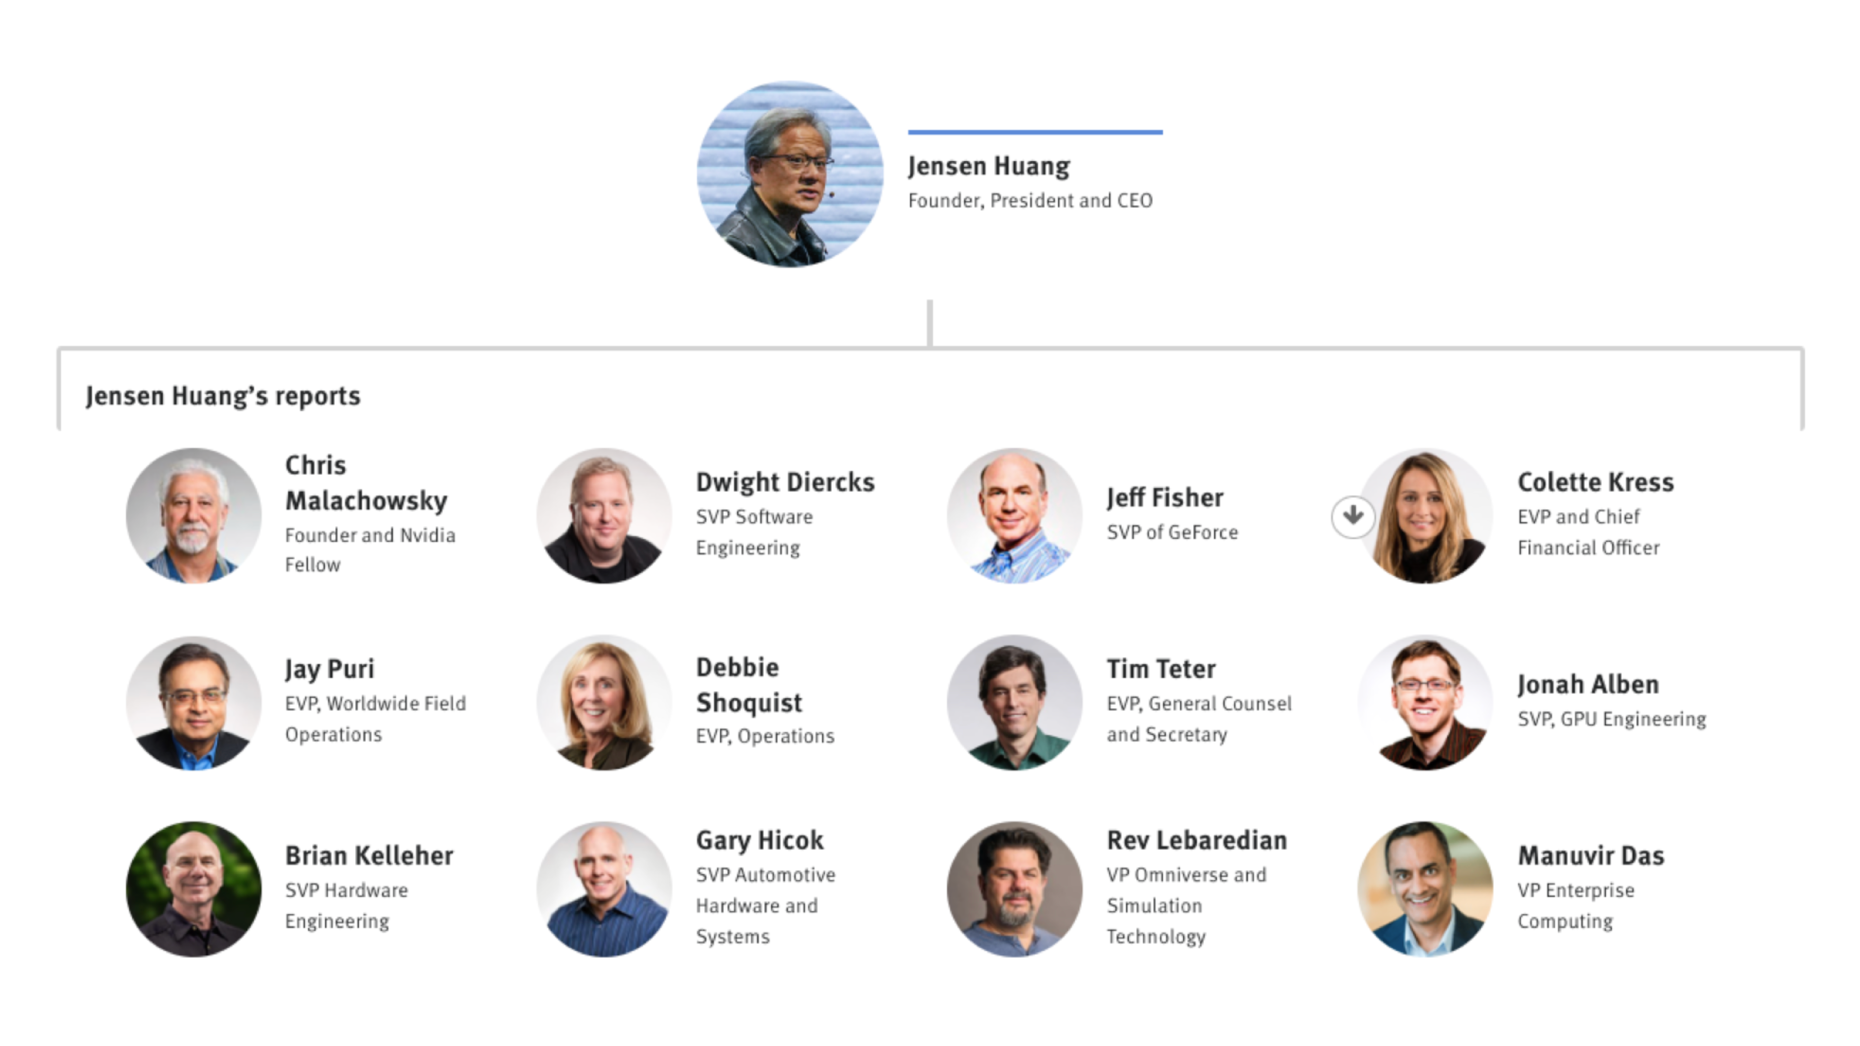
\includegraphics[width=0.7\linewidth]{BSZ_kap_11_2026/by_slide/slide_004/BSZ_kap_11_2026_slide_004_asset_01_image3.png}
  \caption{Den tre-benede skammelen: Decision rights, Performance evaluation, Reward systems -- arkitekturens tre ben. Endring i ett ben krever justering av de andre. (BSZ kap.\ 11, slide 4) [SLIDE]}
\end{figure}

\begin{center}
\renewcommand{\arraystretch}{1.15}
\begin{tabular}{@{}p{3.4cm}p{4.6cm}p{6.0cm}@{}}
\toprule
\textbf{Søyle (ben)} & \textbf{Designvariabel} & \textbf{Hovedmekanisme} \\
\midrule
\SOne\ Decision rights & Hvem beslutter hva (allokering) & Plasser beslutning der spesifik viden sitter \\
\STwo\ Performance eval. & Hva måles, hvordan, av hvem & Erstatte direkte observasjon med kontrollerbart måltall \\
\SThree\ Reward system & Lønn, bonus, opsjoner, karriere & Vri agentens egennytte mot prinsipalens mål \\
\bottomrule
\end{tabular}
\end{center}

\subsection*{Eksempler}
\begin{itemize}
\item \textbf{Equinor (omorganisering 2020/2021):} Skilte ut \emph{Renewables} som egen forretningsenhet (S1), innførte separate KPI-er for fornybar kapasitet og avkastning (S2), og koblet ledelseskompensasjon til transisjonsmål (S3). Tre-benet endring samtidig. [EKS]
\item \textbf{Norsk Hydro -- aluminiumsdivisjonene:} Vertikalt integrert virksomhet med separate divisjoner for Bauxite \& Alumina, Aluminium Metal, og Extruded Solutions. Hver divisjon er profit/investment center (S1), måles på LME-justert margin (S2 -- jf.\ controllability), og bonus knyttes til divisjonsresultat (S3). [EKS]
\item \textbf{IKEA -- franchising:} Beslutningsrett om varehusdrift hos franchisetaker (S1), måles på salg per kvadratmeter og kundetilfredshet (S2), royalty + restprofit til franchisetaker er insentivet (S3). Misalignment-eksempel: hvis konsernet hadde delegert pris (S1) men målt på volum (S2), ville franchisetaker dumpet priser. [EKS]
\item \textbf{Maersk Line vs.\ APM Terminals:} A.P.\ Møller-Mærsk har bevisst skilt skipsdriften (Maersk Line) fra havnedriften (APM Terminals) i to ulike arkitekturer fordi videnstrukturer, kunder og kapitalbehov er forskjellige. [EKS/CASE]
\item \textbf{Mærsk Power-to-X-divisjonen:} Beslutningsrett over teknologivalg og partnervalg ligger i divisjonen (S1), måles som investment center på prosjektets risikojusterte avkastning (S2), og lederkompensasjon koblet til langsiktige milestones (S3). Hadde insentivene bare vært knyttet til kortsiktig EBITDA, ville lederen utsatt store CAPEX-beslutninger -- klassisk misalignment. [CASE]
\end{itemize}

\subsection*{Kobling til søyle og andre teorier}
Modellen \emph{er} de tre søylene -- \SOne\ + \STwo\ + \SThree\ samtidig. Relaterte: \thref{specific-vs-general-knowledge}{Spesifik vs.\ generell viden} (begrunner S1), \thref{agency-costs}{Agentomkostninger} (det modellen minimerer), \thref{principal-agent}{Principal--agent} (grunnrelasjonen), \thref{controllability-principle}{Controllability-prinsippet} (regel for S2), \thref{informativeness-principle}{Informativeness-prinsippet} (regel for S2/S3), \thref{responsibility-centers}{Responsibility centers} (konkret implementering av alle tre), \thref{decision-management-control}{Decision Management vs.\ Decision Control} (strukturer S1), \thref{centralization-vs-decentralization}{Centralisering vs.\ desentralisering} (graden av S1-delegering), \thref{transfer-pricing}{Transfer pricing} (oppstår mellom S2-enheter), \thref{boundaries-of-the-firm}{Boundaries of the firm} (når arkitekturen møter markedet).

\paragraph{Brukt i spørsmål:} Q05.

% !TEX root = ../main.tex
\section{Agentomkostninger (Agency Costs)}\label{thr:agency-costs}

\paragraph{Definisjon.} \emph{Agentomkostninger} (agency costs) er den samlede verditapen som oppstår fordi en agent ikke handler fullt ut i prinsipalens interesse. Jensen \& Meckling (1976) dekomponerer kostnaden i tre komponenter: \textbf{monitoring costs} (prinsipalens utgift til overvåking), \textbf{bonding costs} (agentens utgift til troverdighetssignaler) og \textbf{residual loss} (det gjenværende effektivitetstapet etter at monitoring og bonding er gjort optimalt). [SLIDE]

\subsection*{Forklaring}

I en \thref{principal-agent}{prinsipal--agent}-relasjon skaper agenten verdi for prinsipalen, men har egne preferanser (innsatsaversjon, risikoaversjon, perks, statusbygging). Når informasjon er asymmetrisk, kan ikke prinsipalen presist observere agentens handlinger. Resultatet er at \emph{first-best} (full informasjon, ingen interessekonflikt) ikke er nåbar -- og forskjellen mellom first-best og det realiserte utfallet er den totale agentomkostningen. [SLIDE/BOK]

Den klassiske dekomponeringen lyder:
\[
  \text{Agency costs} \;=\; \underbrace{M}_{\text{monitoring}} \;+\; \underbrace{B}_{\text{bonding}} \;+\; \underbrace{RL}_{\text{residual loss}}.
\]
Prinsipalen velger $M$ og agenten velger $B$ for å minimere \emph{summen} -- ikke for å fjerne $RL$ helt. Det er dyrt å overvåke perfekt, og det er dyrt å binde seg perfekt; en optimal kontrakt aksepterer at en del av tapet blir liggende igjen. [BOK]

\subsubsection*{1. Monitoring costs}
Prinsipalens utgifter til å observere, måle og kontrollere agentens adferd: revisjon, regnskapssystemer, KPI-er, internkontroll, audit committees, eksterne revisorer, rapporteringskrav, IT-overvåking. Eksempel: et sentralisert ERP-system som logger alle innkjøp er monitoring-investering. [SLIDE]

\subsubsection*{2. Bonding costs}
Agentens egne utgifter til å \emph{signalere} eller \emph{garantere} at hun ikke vil utnytte informasjonsovertaket. Eksempler: ledelsesopsjoner som binder lederen til selskapets aksjekurs, restriktive covenants i låneavtaler, deferred compensation, profesjonell sertifisering, frivillige rapporteringsstandarder, og medarbeidereierskap. Bonding er agentens måte å si: ``hvis jeg svikter, taper jeg også''. [SLIDE/BOK]

\subsubsection*{3. Residual loss}
Det gjenværende effektivitetstapet -- forskjellen mellom realisert utfall og first-best -- som blir igjen \emph{etter} at monitoring og bonding er drevet til optimum. Residual loss er ikke et tegn på dårlig kontraktsdesign; det er bevis på at \thref{costless-contracting}{costless contracting} ikke gjelder, og at kompromisset mellom kontroll og kostnad er nådd. [SLIDE]

\subsection*{Tallregnskap fra slide 31 (kap.\ 10)}

\begin{center}
\begin{tabular}{@{}lr@{}}
\toprule
\textbf{Post} & \textbf{Verdi} \\
\midrule
Bruttoverdi av handel & 2\,500 \\
Contracting / out-of-pocket & $-$800 \\
Monitoring costs & $-$400 \\
Bonding costs & $-$400 \\
Residual loss & $-$100 \\
\midrule
Netto verdi $S'$ & 1\,600 \\
\bottomrule
\end{tabular}
\end{center}
\textit{Eksempel fra slide: agentomkostningene reduserer verdien av en handel som i first-best ville vært 2\,500 til 1\,600. Hvis monitoring + bonding hadde vært dyrere enn residual loss de fjerner, ville handelen blitt uattraktiv. [SLIDE]}

\subsection*{Kjerneforutsetninger}
\begin{itemize}
\item \textbf{Asymmetrisk informasjon.} Hvis prinsipalen kunne observere agenten kostnadsfritt, var monitoring overflødig.
\item \textbf{Interessekonflikt.} Hvis agentens nyttefunksjon var sammenfallende med prinsipalens, ville bonding ikke gi mening.
\item \textbf{Risikoaversjon hos agenten} (typisk). Sterkere risikoadeling overfor agent øker bonding-effekten, men også residual loss via redusert insentivstyrke.
\item \textbf{Kontrakter er ufullstendige} ($\Rightarrow$ \thref{costly-contracting}{costly contracting}). Agentomkostninger er en direkte konsekvens av at perfekte tilstandskontrakter ikke kan skrives.
\item \textbf{Begrenset rasjonalitet og positive transaksjonskostnader} (Coase, Williamson).
\end{itemize}

\subsection*{Muligheter (hva forklarer/løser teorien?)}
\begin{itemize}
\item Forklarer \emph{hvorfor virksomheter eksisterer i en bestemt form} -- eierstruktur, kapitalstruktur, kompensasjonsdesign og konsernarkitektur er svar på agentomkostninger.
\item Forklarer hvorfor enkelte transaksjoner organiseres internt (vertikal integrasjon) i stedet for via marked: hvis agentomkostninger ved hierarki $<$ transaksjonskostnader ved marked, internalises transaksjonen.
\item Begrunnelse for sammensetningen av insentivlønn, opsjoner, eierandeler og restriktive covenants -- alt sammen bonding-mekanismer.
\item Begrunnelse for revisor, styreverv, audit committees, intern revisjon -- monitoring-mekanismer.
\item Forutsetning for hele \emph{organizational architecture}-tenkningen: arkitekturen i S1, S2, S3 finnes for å minimere agentomkostninger.
\end{itemize}

\subsection*{Begrensninger og kritikk}
\begin{itemize}
\item \textbf{Måleproblem:} Agentomkostninger er sjelden direkte målbare -- bare residual loss observeres indirekte. Hvor mye som er ``optimalt'' er en teoretisk konstruksjon.
\item \textbf{Risiko for over-monitoring:} For mye overvåking kan ødelegge tillit, intrinsisk motivasjon og kreativitet (crowding-out). Slidene viser ikke dette eksplisitt, men er sentralt i moderne kritikk (Frey, 1997).
\item \textbf{Bonding er ikke gratis for prinsipalen heller:} Insentivlønn og opsjoner overfører risiko til agenten, som krever risikopremie -- jf.\ \thref{informativeness-principle}{informativeness-prinsippet}.
\item \textbf{Opportunistisk re-tolkning:} Ledere kan begrunne nesten enhver utgift som ``monitoring'' eller ``bonding''; konseptene er normative og kan misbrukes.
\item \textbf{Statisk modell:} Klassisk Jensen \& Meckling antar engangsoppsett. Implicit / reputational contracts og gjentatte spill (jf.\ \thref{game-theory}{spilteori}) reduserer agentomkostninger over tid uten å øke $M$ eller $B$.
\item \textbf{Multi-prinsipalproblemer:} Når en agent tjener flere prinsipaler (CEO i børsnotert selskap har aksjonærer, kreditorer, ansatte), blir dekomponeringen mer komplisert.
\end{itemize}

\subsection*{Modell / illustrasjon}

\begin{figure}[H]
\centering
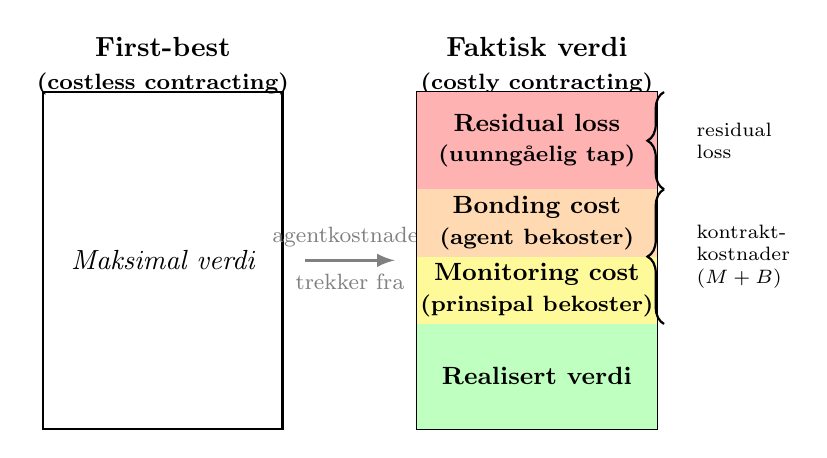
\begin{tikzpicture}[>=latex, scale=0.95, every node/.style={font=\small}]
  % First-best baseline
  \draw[thick] (0,0) rectangle (3.2,4.5);
  \node[font=\bfseries, align=center] at (1.6,4.85) {First-best\\\footnotesize (costless contracting)};
  \node[font=\itshape] at (1.6,2.25) {Maksimal verdi};
  % Pil mellom
  \draw[->, very thick, gray] (3.5,2.25) -- (4.7,2.25);
  \node[gray, font=\footnotesize, above] at (4.1,2.3) {agentkostnader};
  \node[gray, font=\footnotesize, below] at (4.1,2.2) {trekker fra};
  % Andre kolonne: stablet dekomp
  \draw[thick] (5,0) rectangle (8.2,4.5);
  \node[font=\bfseries, align=center] at (6.6,4.85) {Faktisk verdi\\\footnotesize (costly contracting)};
  % Residual loss (øverst)
  \fill[red!30] (5,3.2) rectangle (8.2,4.5);
  \node[font=\bfseries\small, align=center] at (6.6,3.85)
    {Residual loss\\ \footnotesize (uunngåelig tap)};
  % Bonding
  \fill[orange!30] (5,2.3) rectangle (8.2,3.2);
  \node[font=\bfseries\small, align=center] at (6.6,2.75)
    {Bonding cost\\ \footnotesize (agent bekoster)};
  % Monitoring
  \fill[yellow!40] (5,1.4) rectangle (8.2,2.3);
  \node[font=\bfseries\small, align=center] at (6.6,1.85)
    {Monitoring cost\\ \footnotesize (prinsipal bekoster)};
  % Realiserte verdi
  \fill[green!25] (5,0) rectangle (8.2,1.4);
  \node[font=\bfseries\small, align=center] at (6.6,0.7)
    {Realisert verdi};
  % Klammer
  \draw[decorate, decoration={brace, amplitude=6pt}, thick]
    (8.3,3.2) -- (8.3,4.5)
    node[midway, right=8pt, font=\scriptsize, align=left] {residual\\ loss};
  \draw[decorate, decoration={brace, amplitude=6pt}, thick]
    (8.3,1.4) -- (8.3,3.2)
    node[midway, right=8pt, font=\scriptsize, align=left] {kontrakt-\\ kostnader\\ ($M+B$)};
\end{tikzpicture}
\caption{\textbf{Agency cost-dekomponering} (Jensen \& Meckling 1976; BSZ kap.\ 10, slide 7). Avviket fra first-best splittes i tre: \emph{Monitoring costs} (M, prinsipalens overvåking), \emph{Bonding costs} (B, agentens forpliktelser/risiko-bæring) og \emph{Residual loss} (uunngåelig tap pga.\ ikke alle insentivkonflikter kan utelukkes kostnadseffektivt). Total agency cost = $M + B + \text{residual loss}$. [SLIDE]}
\end{figure}

\subsection*{Eksempler}
\begin{itemize}
\item \textbf{Equinor / aksjonærer:} Norsk stat (\textasciitilde 67\%) krever omfattende monitoring via styre, riksrevisjon og åpenhetsregler. CEO-bonding skjer via aksjebasert kompensasjon. Residual loss er likevel synlig: politiske beslutninger om f.eks.\ Trans-Adriatic Pipeline eller fornybarsatsninger som ikke maksimerer NPV. [EKS]
\item \textbf{Mærsk McKinney Møller-fonden:} A.P. Møller-Mærsk har en stiftelseskontrollert eierstruktur som reduserer agentomkostninger ved at langsiktige eiere overvåker direkte; men residual loss kommer i form av begrenset adgang til ekstern kapital ved store satsinger som Power-to-X. [CASE]
\item \textbf{Lehman Brothers (2008):} Eksempel på utilstrekkelig monitoring (svake risikomodeller, manglende styrekontroll) kombinert med pervers bonding (bonus knyttet til kortsiktig P\&L). Residual loss = konkursen selv. [EKS]
\item \textbf{IKEA:} Familiekontrollert via Stichting INGKA Foundation reduserer monitoring-behovet og lar selskapet investere langsiktig. Bonding skjer gjennom kulturelle normer (``IKEA-vägen'') og medarbeideropplæring i Älmhult. [EKS]
\end{itemize}

\subsection*{Kobling til søyle og andre teorier}
Agency costs spenner over alle tre søyler: \SOne\ (hvem som får beslutningsrett bestemmer hvor stor residual loss kan bli), \STwo\ (monitoring \emph{er} prestasjonsmåling), \SThree\ (bonding \emph{er} insentivdesign). Relaterte: \thref{principal-agent}{Principal--agent}, \thref{moral-hazard}{Moral hazard}, \thref{adverse-selection}{Adverse selection}, \thref{costly-contracting}{Costly contracting}, \thref{costless-contracting}{Costless contracting}, \thref{specific-vs-general-knowledge}{Spesifik vs.\ generell viden}, \thref{organizational-architecture}{Organizational architecture}, \thref{informativeness-principle}{Informativeness-prinsippet}.

\paragraph{Brukt i spørsmål:} Q04, Q05, Q06, Q09, Q10, Q11, Q12, Q14.

% !TEX root = ../main.tex
\section{Spesifik vs.\ generell viden}\label{thr:specific-vs-general-knowledge}

\paragraph{Definisjon.} Skillet mellom \emph{spesifik viden} (specific knowledge) og \emph{generell viden} (general knowledge) handler om hvor dyrt det er å overføre kunnskap mellom personer i en organisasjon. Spesifik viden er kostbar å sende oppover (lokal, kontekstuell, taus, tidssensitiv); generell viden er billig å overføre (kvantifiserbar, kodifisert, dokumenterbar). Skillet stammer fra Hayek (1945) ``The Use of Knowledge in Society'' og operasjonaliseres organisasjonsøkonomisk av Jensen \& Meckling (1992). [SLIDE/BOK]

\subsection*{Forklaring}

Hayeks poeng er at viktig kunnskap i et samfunn er \emph{distribuert}: ingen sentral planlegger sitter på all relevant informasjon om lokale forhold, preferanser eller muligheter. Markedet løser dette med \emph{priser} -- prismekanismen aggregerer spredt kunnskap automatisk. Inni en virksomhet finnes det imidlertid ikke priser i samme grad; viden må enten flyttes (kostbart) eller \emph{beslutningsretten} må flyttes til der videnen sitter (også kostbart, fordi det åpner for agentkonflikt). [SLIDE]

Jensen \& Meckling formaliserte trade-off-en i \emph{co-location of knowledge and decision rights}: organisasjonen står overfor to grunnleggende valg:
\begin{enumerate}
\item Sentralisere beslutningen og overføre videnen oppover (sentralisering + informasjonsflyt).
\item Flytte beslutningsretten ned til der videnen er, og overvåke / insentivere lederen (desentralisering + agentstyring).
\end{enumerate}
Ingen av valgene er gratis. Sentralisering taper på dårlig kvalitet av kunnskap (eller høy overføringskost); desentralisering taper på agentkostnader. Optimal organisering balanserer disse to. [BOK]

\subsection*{Konsekvensen for arkitektur}

Dette er hjertet av \thref{organizational-architecture}{organizational architecture}: når beslutningsretten desentraliseres (S1 endres) for å utnytte spesifik viden, må prinsipalen \emph{erstatte} den direkte kontrollen som gikk tapt med to nye mekanismer:
\begin{itemize}
\item \STwo\ \textbf{prestasjonsmåling} -- siden man ikke lenger ser \emph{handlingen}, må man måle \emph{resultatet}.
\item \SThree\ \textbf{insentivstruktur} -- man må kompensere lederen slik at hennes egeninteresse trekker i samme retning som prinsipalens.
\end{itemize}
Spesifik viden er derfor det \emph{drivende} argumentet for hvorfor S1 må følges av S2 og S3. Endrer man bare én søyle, skapes misalignment.

\subsection*{Eksempler på spesifik viden}
\begin{itemize}
\item Lokal markedskunnskap (en butikksjef vet hva nabolagets kunder etterspør).
\item Tidssensitiv kunnskap (trader vet at markedet beveger seg \emph{nå}).
\item Vitenskapelig domenekunnskap (en forsker forstår sitt felt bedre enn lederen).
\item Kunderelasjoner (en account manager kjenner kundens behov over år).
\item Teknisk taus kunnskap (en operatør på et raffineri vet når en pumpe må byttes).
\end{itemize}

\subsection*{Eksempler på generell viden}
\begin{itemize}
\item Aksjekurs i sanntid.
\item Standardiserte regnskapstall.
\item Ferdige rapporter, dashboards, KPI-data.
\item Politikkbeslutninger som kan kodifiseres i regler.
\end{itemize}

\subsection*{Kjerneforutsetninger}
\begin{itemize}
\item Det finnes \emph{en} dimensjon ``kostnaden ved å overføre viden'' som meningsfullt skiller spesifik fra generell.
\item Beslutningsmaker har faktisk insentiv til å bruke videnen riktig (ellers løses ikke problemet ved å flytte beslutningsretten).
\item Prestasjonsmåling kan brukes som substitutt for direkte observasjon når desentralisering velges.
\item Markeder og hierarkier er reelle alternativer (Coase). Dersom verken hierarki eller marked løser videnproblemet, oppstår tredje organiseringsformer (allianser, joint ventures).
\end{itemize}

\subsection*{Muligheter}
\begin{itemize}
\item Forklarer \emph{hvorfor} desentralisering er attraktiv: lokal viden brukes uten kostbar overføring.
\item Forklarer \emph{hvorfor} desentralisering er kostbar: man taper direkte kontroll og må erstatte den med S2/S3.
\item Begrunner valget av \thref{responsibility-centers}{centertype}: cost center ($\to$ lite spesifik viden), profit/investment center ($\to$ mye spesifik viden).
\item Knytter seg til \thref{decision-management-control}{Decision Management vs.\ Decision Control}: når beslutningsmaker ikke bærer fulle formueeffekter, separer initiering/implementering fra ratifisering/monitorering.
\item Forklarer fenomener som franchise, autonome divisjoner, datadrevet sentralisering, og hvorfor IT-revolusjonen har endret balansen (mer kunnskap blir kodifiserbar $\Rightarrow$ generell $\Rightarrow$ rom for re-sentralisering).
\end{itemize}

\subsection*{Begrensninger og kritikk}
\begin{itemize}
\item \textbf{Skillet er glidende.} Mye viden er delvis spesifik og delvis generell -- klassifiseringen er sjelden binær.
\item \textbf{Endogen viden:} Hva som er ``spesifik'' avhenger av hvilke verktøy organisasjonen har bygget for å overføre informasjon. Bedrifter kan investere i å gjøre tidligere spesifik viden generell (BI-systemer, sensorer, AI).
\item \textbf{Strategisk underrapportering:} Lokale ledere kan ha insentiv til å \emph{overdrive} hvor spesifik kunnskapen er, for å beholde beslutningsmakt.
\item \textbf{Modellen sier ikke hvor mye desentralisering som er optimalt.} Den må kombineres med \thref{centralization-vs-decentralization}{decentraliseringsmodellen} (Q06) som balanserer benefits/costs av desentralisering.
\item \textbf{Kollektiv viden / koordinering:} Hayek/Jensen-Meckling håndterer ikke godt situasjoner der \emph{flere} aktører har overlappende, men inkonsistent spesifik viden -- da kreves teamstrukturer og delte beslutningsrom.
\end{itemize}

\subsection*{Modell / illustrasjon}

\begin{figure}[h]
  \centering
  
\includegraphics[width=0.55\linewidth]{BSZ_kap_12_2026/by_slide/slide_018/BSZ_kap_12_2026_slide_018_asset_01_image6.jpeg}
  \caption{Spesifik viden: informasjon som er kostbar å overføre -- sitter lokalt og krever desentralisering av beslutningsrett. (BSZ kap.\ 12, slide 18) [SLIDE]}
\end{figure}

\begin{center}
\begin{tabular}{@{}p{4.6cm}p{4.6cm}p{4.6cm}@{}}
\toprule
\textbf{Forhold} & \textbf{Spesifik viden} & \textbf{Generell viden} \\
\midrule
Overføringskostnad & Høy & Lav \\
Hvor sitter den? & Lokalt, hos operatør / leder & Sentralt eller i system \\
Foretrukken organisering & Desentralisering (flytt beslutningsrett) & Sentralisering (flytt informasjon) \\
Kompletterende mekanismer & S2 + S3 nødvendig & S2/S3 mindre kritisk \\
Egnet centertype & Profit / investment center & Cost / expense center \\
\bottomrule
\end{tabular}
\end{center}
\textit{Co-location av kunnskap og beslutningsrett: enten flytter du videnen til beslutningen, eller beslutningen til videnen. [SLIDE/BOK]}

\subsection*{Eksempler}
\begin{itemize}
\item \textbf{Equinor -- E\&P (Letevirksomhet):} Funn på et nytt prospekt avhenger av lokal geologisk kunnskap som ikke kan kodifiseres uten store tap. Beslutningsretten er derfor delegert til prosjektleder med investment-center-ansvar; selskapet erstatter direkte kontroll med ROACE-måling og opsjonsbasert kompensasjon. [EKS]
\item \textbf{Norges Bank Investment Management (Oljefondet):} Standardisert generell viden (børskurser, indeksvekter) gjør sentralisert beslutningstaking effektivt. Aktive porteføljevalg er likevel desentralisert, fordi seksjonsanalytikere har spesifik viden om enkeltselskaper. [EKS]
\item \textbf{IKEA Älmhult:} Designkunnskap er konsentrert sentralt fordi den kan kodifiseres i tegninger og monteringsanvisninger. Salgsbeslutninger på det enkelte varehus er desentralisert -- lokale preferanser er spesifik viden. [EKS]
\item \textbf{Mærsk Power-to-X:} Valg av elektrolysørteknologi krever spesifik teknisk viden hos PtX-divisjonen, ikke i konsernledelsen. Derfor er beslutningsrett om teknologipartner delegert nedover; kompensasjonen knyttes til prosjektets NPV/IRR (investment center) for å løse den nye agentkonflikten. [CASE]
\end{itemize}

\subsection*{Kobling til søyle og andre teorier}
Søyle: Skillet er logisk grunn for hele \SOne\ (allokering av beslutningsrett); via følgemekanismene driver det også \STwo\ og \SThree. Relaterte: \thref{principal-agent}{Principal--agent}, \thref{agency-costs}{Agentomkostninger}, \thref{organizational-architecture}{Organizational architecture}, \thref{centralization-vs-decentralization}{Centralisering vs.\ desentralisering}, \thref{decision-management-control}{Decision Management vs.\ Decision Control}, \thref{responsibility-centers}{Responsibility centers}.

\paragraph{Brukt i spørsmål:} Q02, Q05, Q06, Q07, Q11, Q12.

% Q06 theories
% !TEX root = ../main.tex
\section{Centralisering vs.\ desentralisering}\label{thr:centralization-vs-decentralization}

\paragraph{Definisjon.} \emph{Sentralisering} betyr at beslutningsretten holdes høyt oppe i hierarkiet (CEO, toppledelse, konsernfunksjoner), mens \emph{desentralisering} betyr at beslutningsretten delegeres nedover til lokale ledere, team eller medarbeidere. Trade-off-en mellom de to er det første benet (\SOne) i \thref{organizational-architecture}{organizational architecture} -- og er drevet av skillet mellom \thref{specific-vs-general-knowledge}{spesifik og generell viden} (Hayek 1945; Jensen \& Meckling 1992; BSZ kap.\ 12). [SLIDE/BOK]

\subsection*{Forklaring}

Sentralisering og desentralisering er endepunktene på et kontinuum, ikke et binært valg. I praksis er enhver bedrift en blanding: enkelte beslutninger (kapitalstruktur, akkvisisjoner, store CAPEX) holdes sentralt, mens andre (prising på filialen, ansettelser, daglig drift) delegeres. Spørsmålet er hvor \emph{graden} av desentralisering skal ligge -- formalisert i \thref{optimal-decentralization-model}{optimal-desentraliseringsmodellen}. [SLIDE]

Hayek (1945) er det teoretiske utgangspunktet: relevant viden i en organisasjon er distribuert -- ingen toppleder vet alt. Når mye viden er \emph{spesifik} (kostbar å overføre), gir det mening å flytte beslutningen til der videnen sitter, fremfor å forsøke å løfte videnen oppover. Når videnen derimot er \emph{generell} (kvantifiserbar, kodifiserbar, billig å sende), kan beslutningen sentraliseres og dra nytte av stordriftsfordeler og bedre koordinering. Jensen \& Meckling (1992) formaliserer dette som ``co-location of knowledge and decision rights''. [BOK]

\subsection*{Fordele ved desentralisering}
\begin{itemize}\setlength{\itemsep}{2pt}
\item \textbf{Bedre bruk av lokal (spesifik) viden.} Lokale ledere kjenner kunder, markeder, prisfølsomhet og operasjonelle forhold som toppledelsen ikke har tilgang til. [SLIDE]
\item \textbf{Tidsbesparelse for senior management.} Toppledelsen frigjøres til strategi og langsiktig planlegging i stedet for å drukne i operative detaljer. [SLIDE]
\item \textbf{Motivasjon og opplæring.} Delegasjon gir ansvar og eierskap, øker motivasjon og utvikler fremtidige ledere -- delegering er en organisatorisk talentpipeline. [SLIDE]
\item \textbf{Raskere respons på lokale endringer} (kortere informasjonskjede $\Rightarrow$ kortere beslutningsvei).
\item \textbf{Mindre overload på toppledelsen} (begrenset prosesseringskapasitet -- ``bounded rationality'').
\end{itemize}

\subsection*{Ulemper ved desentralisering}
\begin{itemize}\setlength{\itemsep}{2pt}
\item \textbf{\thref{agency-costs}{Agentomkostninger}.} Lokale ledere kan forfølge egne interesser (perks, empire-building, slacking) når kontrollen reduseres. [SLIDE]
\item \textbf{Koordinasjonskostnader.} Enheter kan mislykkes i å koordinere, duplisere aktiviteter eller kannibalisere hverandres salg. Disse kostnadene vokser typisk \emph{konveks} i graden av desentralisering. [SLIDE]
\item \textbf{Tap av stordriftsfordeler.} Sentralisert innkjøp, IT, HR og økonomistyring gir lavere enhetskostnad enn parallelle desentraliserte funksjoner. [SLIDE]
\item \textbf{Inkonsistente beslutninger / brand-risiko} (forskjellige enheter behandler kunder ulikt).
\item \textbf{Vanskeligere kunnskapsdeling på tvers} -- spesifik viden forblir lokal hvis ikke bevisst håndtert.
\end{itemize}

\subsection*{Fordele ved sentralisering (speilbilde)}
\begin{itemize}\setlength{\itemsep}{2pt}
\item Bedre koordinering, stordriftsfordeler, konsistens og lavere agentomkostninger ved homogen drift.
\item Egnet når videnen er \emph{generell} -- f.eks.\ standardiserte regnskaps- og IT-systemer, konsernfinans, M\&A.
\end{itemize}

\subsection*{Ulemper ved sentralisering}
\begin{itemize}\setlength{\itemsep}{2pt}
\item Dårlig utnyttelse av spesifik lokal viden $\Rightarrow$ feilbeslutninger.
\item Lange beslutningsveier og treghet.
\item Toppledelsesoverload og motivasjonstap nede i organisasjonen.
\end{itemize}

\subsection*{Trade-off-en (kjernen)}
Trade-off-en kan oppsummeres slik: \emph{Desentralisering gir bedre informasjon i beslutningen, men dårligere insentivlinje. Sentralisering gir bedre insentivlinje, men dårligere informasjon.} Hver gang man flytter en beslutning nedover, må man kompensere med to ting: \STwo\ prestasjonsmåling (siden direkte observasjon faller bort) og \SThree\ insentivstruktur (siden lederen nå har handlingsrom). Endrer man bare \SOne\ uten å justere de to andre, faller skammelen og residual loss eksploderer. [BOK]

\subsection*{Kjerneforutsetninger}
\begin{itemize}\setlength{\itemsep}{2pt}
\item Viden er distribuert (Hayek) og delvis spesifik (Jensen \& Meckling).
\item Beslutningsrett kan faktisk allokeres -- den er ikke ``naturgitt'' bestemt.
\item Prestasjonsmåling kan brukes som substitutt for direkte observasjon når desentralisering velges.
\item Marginale fordeler og kostnader ved desentralisering er meningsfulle størrelser (nødvendig for modellen i Q06).
\item Komplementaritet i arkitekturen: \SOne, \STwo\ og \SThree\ må designes samtidig (Milgrom \& Roberts 1995).
\end{itemize}

\subsection*{Muligheter}
\begin{itemize}\setlength{\itemsep}{2pt}
\item Begrunner valget av \thref{responsibility-centers}{centertype} -- mer desentralisering $\Rightarrow$ profit/investment center; mer sentralisering $\Rightarrow$ cost/expense center.
\item Forklarer fenomener som franchise (sterk desentralisering med output-kontrakter), holdingstrukturer, autonome divisjoner.
\item Forklarer hvorfor IT- og dataplattformer endrer balansen: generell viden vokser $\Rightarrow$ argument for re-sentralisering (analytics, plattformøkonomi).
\item Knytter seg til \thref{decision-management-control}{Decision Management vs.\ Decision Control}: selv ved sterk desentralisering bør initiering/implementering skilles fra ratifisering/monitorering når lederen ikke bærer fulle formueeffekter.
\end{itemize}

\subsection*{Begrensninger og kritikk}
\begin{itemize}\setlength{\itemsep}{2pt}
\item \textbf{Kontinuum, ikke binær.} Begrepet ``desentralisering'' dekker et spekter; samme bedrift er ofte desentralisert på enkelte dimensjoner og sentralisert på andre. Modellen taper presisjon hvis man bruker den unidimensjonalt.
\item \textbf{Endogen viden.} Hva som er spesifik viden avhenger av hvilke IT-, måle- og rapporteringssystemer bedriften har bygget. Spesifik viden kan gjøres generell over tid (sensorer, datavarehus, AI) -- trade-off-en flytter seg.
\item \textbf{Strategisk underrapportering.} Lokale ledere har egeninteresse i å \emph{overdrive} hvor spesifik deres viden er, for å beholde beslutningsmakt. Modellen tar ikke høyde for dette.
\item \textbf{Statisk modell.} Trade-off-en sier ikke noe om \emph{tilpasningshastighet} -- bedrifter som ikke endrer arkitektur når omgivelsene endres, blir slått av ``economic Darwinism''.
\item \textbf{Influence costs.} Når beslutningsrett er konsentrert sentralt, oppstår lobbying og politisk adferd som er en egen klasse kostnader (BSZ kap.\ 12) -- ikke fanget i den enkle B--A--C-modellen.
\item \textbf{Koordinering på tvers av enheter.} Ren delegasjon håndterer ikke godt situasjoner med eksternaliteter; da må man supplere med interne markeder, \thref{transfer-pricing}{transfer pricing} eller komitéstrukturer.
\end{itemize}

\subsection*{Modell / illustrasjon}

\begin{figure}[h]
  \centering
  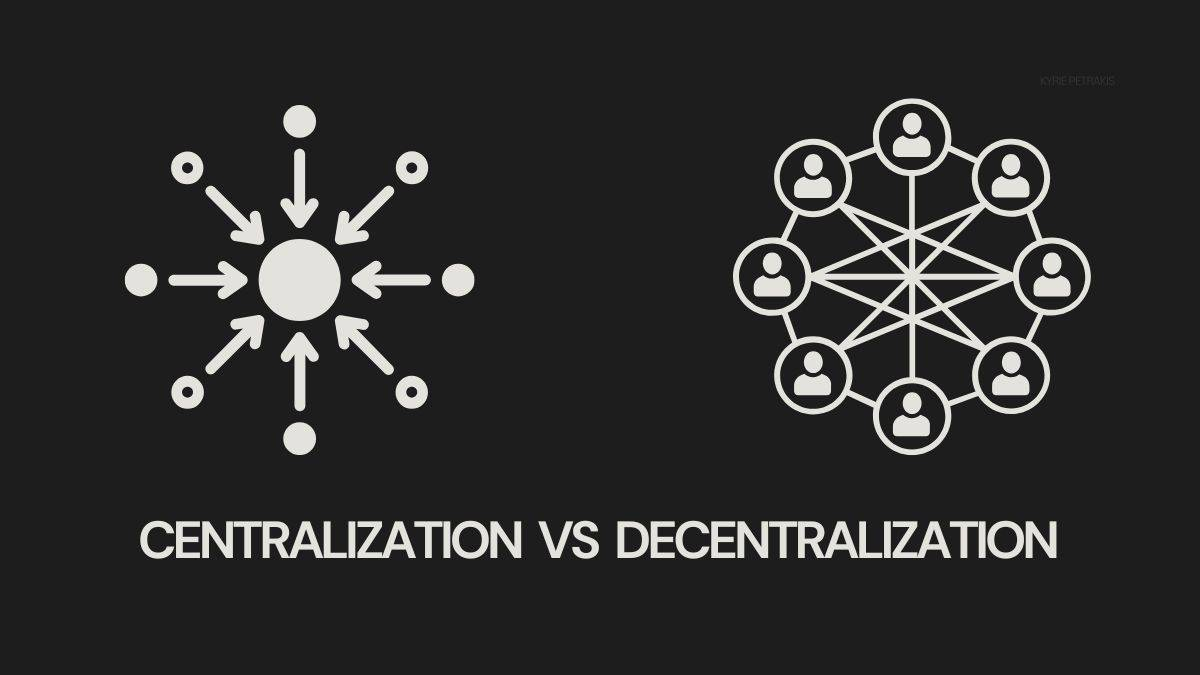
\includegraphics[width=0.6\linewidth]{BSZ_kap_12_2026/by_slide/slide_004/BSZ_kap_12_2026_slide_004_asset_01_image1.jpeg}
  \caption{Sentralisering (venstre: én sentral beslutningsnode) vs.\ desentralisering (høyre: distribuert nettverk av beslutningstakere). BSZ kap.\ 12, slide 4. [SLIDE]}
\end{figure}

\begin{center}
\renewcommand{\arraystretch}{1.15}
\begin{tabular}{@{}p{4.3cm}p{5.0cm}p{5.0cm}@{}}
\toprule
\textbf{Dimensjon} & \textbf{Sentralisering} & \textbf{Desentralisering} \\
\midrule
Hvor sitter beslutningen? & Toppledelse / hovedkontor & Lokal leder / team \\
Forutsetter & Generell viden, lavt behov for tilpasning & Spesifik viden, høyt behov for tilpasning \\
Hovedfordel & Koordinering, stordrift, kontroll & Lokal kunnskap, hurtighet, motivasjon \\
Hovedkostnad & Tap av lokal kunnskap, treghet & Agentkostnader, koordineringssvikt \\
Krav til S2/S3 & Mindre kritisk & Helt essensielt \\
Typisk centertype & Cost / expense center & Profit / investment center \\
\bottomrule
\end{tabular}
\end{center}

\subsection*{Eksempler}
\begin{itemize}\setlength{\itemsep}{2pt}
\item \textbf{Equinor:} Leteprosjekter er desentralisert (geologisk spesifik viden), mens konsernfinans og kapitalallokering er sentralisert (generell viden, stordriftsfordeler). [EKS]
\item \textbf{IKEA:} Produktdesign er sentralisert i \"Almhult (kodifiserbar i tegninger), mens salgsbeslutninger per varehus er desentralisert (lokale preferanser). [EKS]
\item \textbf{McDonald's vs.\ Starbucks:} McDonald's bruker franchise (vidtgående desentralisering med standardiserte kontrakter); Starbucks driver kafeer som heleide enheter (mer sentralisert), nettopp fordi kundeopplevelsen krever konsistens. [EKS]
\item \textbf{Mærsk PtX:} Teknologivalg og partnervalg er delegert nedover (spesifik kjemi-/prosesskompetanse), mens CAPEX-godkjenning og finansiering holdes sentralt. [CASE]
\end{itemize}

\subsection*{Kobling til søyle og andre teorier}
Søyle: Trade-off-en er kjernen i \SOne\ (decision rights) og kobler S1 til \STwo\ og \SThree\ via behovet for å erstatte direkte kontroll. Relaterte: \thref{specific-vs-general-knowledge}{Spesifik vs.\ generell viden} (driveren), \thref{optimal-decentralization-model}{Optimal decentraliseringsmodell} (kvantifisering), \thref{agency-costs}{Agentomkostninger} (kostnadssiden), \thref{organizational-architecture}{Organizational architecture} (helheten), \thref{responsibility-centers}{Responsibility centers} (implementering), \thref{decision-management-control}{Decision Management vs.\ Decision Control} (separasjon ved svake formueeffekter).

\paragraph{Brukt i spørsmål:} Q06.

% !TEX root = ../main.tex
\section{Optimal decentraliseringsmodell}\label{thr:optimal-decentralization-model}

\paragraph{Definisjon.} \emph{Optimal decentraliseringsmodell} er BSZ-rammeverket (kap.\ 12) som operasjonaliserer trade-off-en mellom \thref{centralization-vs-decentralization}{sentralisering og desentralisering} ved å sette opp en nettofordel-funksjon i graden av desentralisering $D$, og finne den graden $D^*$ som maksimerer nettofordelen ved å sette marginal fordel lik marginal kostnad. [SLIDE/BOK]

\subsection*{Forklaring}

La $D \in [0, D_{\max}]$ angi graden av desentralisering (0 = full sentralisering, $D_{\max}$ = full desentralisering). Modellen antar at: [SLIDE]
\begin{itemize}\setlength{\itemsep}{2pt}
\item Fordelene ved desentralisering (bedre bruk av lokal viden) vokser \emph{lineært} i $D$ med rate $B > 0$. Total fordel: $B \cdot D$.
\item Agentkostnadene (linje for direkte ansvarstap) vokser \emph{lineært} i $D$ med rate $A > 0$. Total kostnad ved agentkonflikt: $A \cdot D$.
\item Koordineringskostnadene vokser \emph{kvadratisk} i $D$ med koeffisient $C > 0$. Dette fanger at koordineringsproblemer eskalerer raskt -- flere autonome enheter $\Rightarrow$ kvadratisk flere grensesnitt: $C \cdot D^2$.
\end{itemize}

\paragraph{Nettofordel.} Nettofordelen av desentralisering er
\[
\mathrm{NB}(D) \;=\; B\,D \;-\; A\,D \;-\; C\,D^{2}.
\]

\paragraph{First-order condition.} Vi deriverer og setter lik null:
\[
\frac{d\,\mathrm{NB}}{dD} \;=\; B - A - 2\,C\,D \;=\; 0 \;\;\Longrightarrow\;\; \boxed{\;D^{*} \;=\; \frac{B-A}{2C}\;}.
\]

Andreordens-betingelsen er oppfylt: $d^2\mathrm{NB}/dD^2 = -2C < 0$, så $D^*$ er et maksimum. NB$(D)$ er en konkav parabel som tilskjærer null ved $D=0$ og ved $D = (B-A)/C$, og topper seg midtveis -- ved $D^*$. [BOK]

\subsection*{Komparativ statikk}
\begin{itemize}\setlength{\itemsep}{2pt}
\item $\dfrac{\partial D^*}{\partial B} = \dfrac{1}{2C} > 0$ -- jo større marginal nytte av lokal viden, desto mer desentraliser. Bransjer med mye spesifik viden (E\&P, konsulent, R\&D) ligger høyt på $D^*$.
\item $\dfrac{\partial D^*}{\partial A} = -\dfrac{1}{2C} < 0$ -- jo høyere marginal agentkostnad (svak måling, svake insentiver, opportunistiske ledere), desto mer sentralisering.
\item $\dfrac{\partial D^*}{\partial C} = -\dfrac{B-A}{2C^2} < 0$ (når $B>A$) -- jo dyrere koordinering, desto mer sentralisering. Sterkt integrerte verdikjeder (stålverk, raffineri) har høyt $C$ og lavt $D^*$.
\item Hvis $B \le A$, blir $D^* \le 0$ -- da skal man ikke desentralisere i det hele tatt (marginal fordel av lokal viden er allerede mindre enn marginal agentkostnad ved $D=0$).
\end{itemize}

\subsection*{Numeriske eksempler}
\begin{itemize}\setlength{\itemsep}{2pt}
\item \textbf{Eks.\ 1:} $B=10, A=2, C=4 \Rightarrow D^* = (10-2)/(2\cdot 4) = 1.0$. Maksimal NB $= 10\cdot 1 - 2\cdot 1 - 4\cdot 1^2 = 4$.
\item \textbf{Eks.\ 2 (mer agentkost):} $B=10, A=6, C=4 \Rightarrow D^* = 0.5$. NB $= 5 - 3 - 1 = 1$. Høyere agentkost trekker $D^*$ ned.
\item \textbf{Eks.\ 3 (mer koordineringskost):} $B=10, A=2, C=8 \Rightarrow D^* = 0.5$. NB $= 5 - 1 - 2 = 2$. Høyere $C$ trekker $D^*$ ned.
\end{itemize}

\subsection*{Kjerneforutsetninger}
\begin{itemize}\setlength{\itemsep}{2pt}
\item Fordeler og kostnader er separable og kan måles på samme skala (kroner).
\item Marginal fordel av desentralisering er konstant (lineær) -- forenkling.
\item Koordineringskostnaden er konveks i $D$ -- begrunnet i at antall grensesnitt vokser kvadratisk i antall enheter.
\item Agentkostnaden er lineær -- forenkling som forutsetter at \STwo/\SThree-systemene oppskaleres proporsjonalt med $D$.
\item Beslutter (prinsipalen) har målet å maksimere total firmaverdi (NB), ikke fordelingen mellom prinsipal og agent.
\item Parametrene $B, A, C$ er eksogene -- de avhenger ikke selv av $D$ (en sterk forenkling; se kritikk).
\end{itemize}

\subsection*{Muligheter}
\begin{itemize}\setlength{\itemsep}{2pt}
\item Gir en kvantitativ logikk for hvorfor optimal grad av desentralisering ligger \emph{innenfor} et kontinuum, ikke i et hjørne (0 eller maks).
\item Gir entydige komparativ-statikk-prediksjoner som er empirisk testbare: bransjer/firmaer med høy $B$ skal være mer desentralisert.
\item Knytter direkte til \thref{specific-vs-general-knowledge}{Hayek/J\&M-rammeverket} via parameteren $B$ (marginalverdien av lokal viden) og til \thref{agency-costs}{agentomkostninger} via parameteren $A$.
\item Forklarer hvorfor bedrifter re-sentraliserer når koordineringsbehovet stiger (globale plattformer, fellestjenester) -- $C$ øker.
\item Kan utvides: substituere $A$ med en funksjon av kvaliteten på \STwo\ og \SThree\ -- da kobles modellen direkte til \thref{organizational-architecture}{arkitekturen}.
\end{itemize}

\subsection*{Begrensninger og kritikk}
\begin{itemize}\setlength{\itemsep}{2pt}
\item \textbf{Sterke funksjonsformer.} Antakelsene om lineær fordel og kvadratisk kostnad er stilisterte; virkelige $B$- og $C$-funksjoner kan være ikke-monotone (f.eks.\ stordriftsulemper ved \emph{for} stor sentralisering -- bureaucracy cost).
\item \textbf{$D$ er endimensjonalt.} I praksis er desentralisering flerdimensjonalt -- ulike beslutningsklasser (prising, ansettelse, CAPEX) har hver sin optimale $D$.
\item \textbf{Endogene parametre.} $A$ avhenger av hvor godt \STwo/\SThree\ er designet; $C$ avhenger av IT- og koordineringssystemer; $B$ avhenger av om videnen forblir spesifik eller blir kodifisert. Behandler man dem som konstanter, mister man at de er ledelses\emph{valg}.
\item \textbf{Ignorerer \emph{influence costs}.} Politisk lobbying og rent-seeking er ikke fanget; spesielt relevant ved sterk sentralisering.
\item \textbf{Statisk.} Modellen sier ingenting om tilpasningshastighet eller adaptive omgivelser -- ``economic Darwinism'' antyder at $D^*$ skifter over tid.
\item \textbf{Ingen risiko/risikoaversjon.} Mer desentralisering overfører mer risiko til lokale ledere; en risiko-justert modell ville tilpasse $A$ med en risikopremie.
\item \textbf{Empirisk parameterskjønn.} $B, A, C$ er sjelden direkte målbare; modellen brukes derfor mest \emph{kvalitativt} som ramme for å diskutere hvilken vei optimal $D$ skifter.
\end{itemize}

\subsection*{Modell / illustrasjon}

% NB: TikZ-figur. Krever \usepackage{tikz} i preamble — orchestrator må legge til. Fallback hvis tikz ikke er lastet: kommentér ut blokken nedenfor; tabellen og formelen står seg alene.
\begin{figure}[H]
\centering
\begin{tikzpicture}[scale=1.0]
  % Akser
  \draw[->, thick] (0,0) -- (7.5,0) node[right] {$D$ (grad av desentralisering)};
  \draw[->, thick] (0,0) -- (0,5) node[above] {kr};
  % Marginal Benefit-linje (horisontal): MB = B
  \draw[thick, blue!70!black] (0,4) -- (7,4) node[right] {$\mathrm{MB} = B$};
  % Marginal Cost-linje: MC = A + 2CD, starter på A=1, stiger med stigning 2C=1
  \draw[thick, red!70!black] (0,1) -- (4,5) node[right] {$\mathrm{MC} = A + 2CD$};
  % Krysningspunkt: ved B=4, A+2CD=4 => 1+1*D=4 => D=3
  \draw[dashed] (3,0) -- (3,4);
  \filldraw[black] (3,4) circle (1.5pt);
  \node[below] at (3,0) {$D^{*}$};
  \node[left] at (0,4) {$B$};
  \node[left] at (0,1) {$A$};
  % Optimum-merking
  \node[above right] at (3,4) {\small Optimum};
\end{tikzpicture}
\caption{Marginal-resonnementet: optimum der $\mathrm{MB} = \mathrm{MC}$, dvs.\ $B = A + 2CD^{*}$, som gir $D^{*} = (B-A)/(2C)$. Konstant marginal fordel av lokal viden ($B$) møter stigende marginal kostnad ($A + 2CD$) fra agent- og koordineringskostnader. [SLIDE/EGEN]}
\end{figure}

\begin{figure}[H]
\centering
\begin{tikzpicture}[scale=1.0]
  % Akser for NB-parabel
  \draw[->, thick] (0,0) -- (7.5,0) node[right] {$D$};
  \draw[->, thick] (0,-0.5) -- (0,5.2) node[above] {$\mathrm{NB}(D)$};
  % Parabel: NB = (B-A)D - CD^2; med B-A=3, C=0.5 => topp ved D=3, NB(3)=4.5
  \draw[thick, violet!80!black, domain=0:6, smooth, samples=80, variable=\x]
    plot ({\x},{3*\x - 0.5*\x*\x});
  % Topp ved D*=3
  \draw[dashed] (3,0) -- (3,4.5);
  \filldraw[black] (3,4.5) circle (1.5pt);
  \node[below] at (3,0) {$D^{*}$};
  \node[above right] at (3,4.5) {\small $\mathrm{NB}_{\max}$};
  \node[below] at (6,0) {$D = (B-A)/C$};
\end{tikzpicture}
\caption{Nettofordel-parabelen $\mathrm{NB}(D) = (B-A)D - CD^{2}$. Konkav, topper ved $D^{*} = (B-A)/(2C)$, og krysser null ved $D = 0$ og $D = (B-A)/C$. [SLIDE/EGEN]}
\end{figure}

\subsection*{Eksempler}
\begin{itemize}\setlength{\itemsep}{2pt}
\item \textbf{Equinor leting:} Høy $B$ (geologisk spesifik viden), moderat $A$ (gode måltall: ROACE, suksessrate), moderat $C$ $\Rightarrow$ relativt høyt $D^*$, prosjektleder er investment center. [EKS]
\item \textbf{Stålverk (integrert prosess):} Lavt $B$ (relativt generell prosessviden), høy $C$ (tett integrert verdikjede) $\Rightarrow$ lavt $D^*$, sterkt sentralisert. [EKS]
\item \textbf{Konsulentselskap:} Høy $B$ (klientspesifik viden), lav $C$ (oppdrag er løst koblet) $\Rightarrow$ høyt $D^*$, partnermodell med vidtgående lokal autonomi. [EKS]
\item \textbf{Mærsk PtX:} Høy $B$ (teknisk spesifik kompetanse), men også høy $A$ for største CAPEX-beslutninger (svak måling pga.\ lang horisont) $\Rightarrow$ \emph{splittet} struktur: teknologivalg desentralisert, kapitalallokering sentralisert. [CASE]
\end{itemize}

\subsection*{Kobling til søyle og andre teorier}
Søyle: Modellen er det kvantitative verktøyet for \SOne\ (decision rights) og styrer indirekte behovet for \STwo\ og \SThree\ via parameteren $A$. Relaterte: \thref{centralization-vs-decentralization}{Centralisering vs.\ desentralisering} (kvalitativ trade-off), \thref{specific-vs-general-knowledge}{Spesifik vs.\ generell viden} (driveren for $B$), \thref{agency-costs}{Agentomkostninger} (driveren for $A$), \thref{organizational-architecture}{Organizational architecture} (rammen), \thref{decision-management-control}{Decision Management vs.\ Decision Control} (komplementær mekanisme når $A$ er høy).

\paragraph{Brukt i spørsmål:} Q06.

% Q07 theories
% !TEX root = ../main.tex
\section{Decision Management vs.\ Decision Control}\label{thr:decision-management-control}

\paragraph{Definisjon.} Fama \& Jensen (1983) deler en hvilken som helst beslutningsprosess i fire trinn og grupperer dem i to roller: \emph{Decision Management} = (1) \textbf{Initiation} (generere forslag) + (3) \textbf{Implementation} (eksekvere), og \emph{Decision Control} = (2) \textbf{Ratification} (godkjenne) + (4) \textbf{Monitoring} (evaluere/sanksjonere). Kjerneideen er at når beslutningstakeren \emph{ikke} er \thref{residual-claimants}{residual claimant} (ikke bærer fulle formueeffekter av sine egne beslutninger), bør Management og Control \emph{separeres} på ulike personer/organer for å begrense opportunisme og redusere agentomkostninger. [SLIDE/BOK]

\subsection*{Forklaring}

Beslutninger inni en virksomhet er sjelden ``ett valg''; de er en sekvens. En divisjonsleder \emph{foreslår} et investeringsprosjekt (Initiation), styret eller en CAPEX-komité \emph{godkjenner} det (Ratification), prosjektorganisasjonen \emph{gjennomfører} det (Implementation), og styret/internrevisjon/aksjonærene \emph{måler resultatet og sanksjonerer} (Monitoring). Det er denne sekvensen som er Fama \& Jensens 4-trinns-modell. [SLIDE]

Når én og samme person både initierer, godkjenner, gjennomfører og monitorer egne beslutninger, har hun frie tøyler. Hvis hun samtidig ikke fanger residualen (er ansatt, ikke eier), vil hun rasjonelt velge beslutninger som maksimerer egennytte (prestige-prosjekter, empire building, lave krav, skjul av dårlige nyheter) på bekostning av residualkravshavere. Løsningen er institusjonell \emph{rolledeling}: la den med \thref{specific-vs-general-knowledge}{spesifik viden} stå for Management (Initiation + Implementation), og la et organ som representerer residualkravshaverne stå for Control (Ratification + Monitoring). Dette er hvorfor styret ikke driver selskapet, men ratifiserer CEOs forslag og monitorerer utfallet. [SLIDE/BOK]

I små virksomheter der \emph{én person er både beslutningstaker og residual claimant} (gründer-eier, enkelmannsforetak, lite partnerskap), gir det ingen mening å separere -- separasjon koster informasjonsoverføring uten å løse noe agentproblem. Da kan management og control samles. Trade-off-en er derfor: tap av lokal viden ved separasjon (forslaget filtreres oppover) vs.\ tap fra opportunisme uten separasjon. [BOK]

\subsection*{Kjerneforutsetninger}
\begin{itemize}
\item Beslutninger kan dekomponeres i fire identifiserbare trinn.
\item Beslutningstaker har egne preferanser som kan avvike fra residualkravshaverens (\thref{principal-agent}{principal-agent}-relasjon).
\item Spesifik viden om Initiation og Implementation sitter typisk \emph{lavt} i organisasjonen (lokal kunnskap).
\item Ratification og Monitoring kan utføres med generell viden (måltall, budsjetter, rapporter) -- ellers ville styret aldri kunne ratifisere noe.
\item Det er kostbart, men mulig, å la to ulike organer/personer eie hver sin halvdel av prosessen.
\item Residualkravshaverens insentiv til verdimaksimering driver kvaliteten på Control.
\end{itemize}

\subsection*{Muligheter}
\begin{itemize}
\item Forklarer hvorfor styreutvalg (revisjons-, kompensasjons-, risikoutvalg) finnes: de er institusjonalisert Control over CEOs Management.
\item Forklarer hvorfor virksomheter har CAPEX-terskler: under terskel kan divisjonsleder både initiere og ratifisere; over terskel må styret ratifisere -- typisk separasjon der formueeffekter blir store.
\item Forklarer hvorfor universitetstenure-komiteer, NGO-styrer, kirkesyn og dommerpaneler eksisterer: i \emph{ikke-profitt}-organisasjoner er ikke residualkravshaveren naturlig, og separasjon brukes som substitutt for markedets disiplin.
\item Gir et diagnoseverktøy: når en skandale skjer, spør \emph{hvilket av de fire trinnene sviktet}? Wells Fargo (2016) = svikt i Monitoring; Lehman (2008) = svikt i Ratification og Monitoring; Enron (2001) = revisor (PwC) kollapset Control-rollen.
\item Komplementerer \thref{organizational-architecture}{organizational architecture}: separasjon av management/control er en konkret S1-design som krever S2 (måltall som styret kan ratifisere/monitorere) og S3 (insentiver som disiplinerer Management).
\end{itemize}

\subsection*{Begrensninger og kritikk}
\begin{itemize}
\item \textbf{Asymmetrisk informasjon mot Control:} Styret kan ikke ratifisere eller monitorere effektivt hvis det ikke har samme viden som ledelsen. Boards kan derfor bli ``rubber stamps'' -- formell separasjon uten reell kontroll.
\item \textbf{Kostnader ved separasjon:} Hver ratifikasjonsrunde forsinker, krever rapportering og bryter informasjonsflyten. I små, tidssensitive virksomheter blir Control-leddet en flaskehals.
\item \textbf{Collusion:} Hvis Control-organet kapres av Management (CEO velger sitt eget styre, eller styrets bonus følger CEOs lønn), kollapser separasjonen i praksis selv om den eksisterer formelt.
\item \textbf{Multi-prinsipal-problem:} I ikke-profitt-organisasjoner uten klare residualkravshavere (universiteter, statseide selskaper, stiftelser) er det uklart \emph{hvem} Control-organet skal optimalisere for.
\item \textbf{Glemmer team-beslutninger:} Modellen er en lineær 4-trinns-sekvens; mange reelle beslutninger er iterative og distribuerte mellom mange aktører samtidig.
\item \textbf{Influence costs:} Når Management vet at Control skal ratifisere, brukes ressurser på lobby, presentasjonspakker og selektiv informasjon -- ren effektivitetstap (Milgrom \& Roberts).
\end{itemize}

\subsection*{Modell / illustrasjon}

\begin{figure}[H]
\centering
\begin{tikzpicture}[>=latex, every node/.style={font=\small}, node distance=0.5cm]
  % Fire trinn-bokser
  \node[draw, rounded corners, thick, fill=blue!15, minimum width=2.6cm, minimum height=1.0cm, align=center] (S1) {\bfseries 1. Initiation\\ \footnotesize forslag, ideer};
  \node[draw, rounded corners, thick, fill=red!15, minimum width=2.6cm, minimum height=1.0cm, align=center, right=0.6cm of S1] (S2) {\bfseries 2. Ratification\\ \footnotesize godkjenning};
  \node[draw, rounded corners, thick, fill=blue!15, minimum width=2.6cm, minimum height=1.0cm, align=center, right=0.6cm of S2] (S3) {\bfseries 3. Implementation\\ \footnotesize gjennomføring};
  \node[draw, rounded corners, thick, fill=red!15, minimum width=2.6cm, minimum height=1.0cm, align=center, right=0.6cm of S3] (S4) {\bfseries 4. Monitoring\\ \footnotesize måling, evaluering};
  % Piler mellom
  \draw[->, thick] (S1) -- (S2);
  \draw[->, thick] (S2) -- (S3);
  \draw[->, thick] (S3) -- (S4);
  % DM-klammer under blå-trinn (Management = Initiation + Implementation)
  \draw[decorate, decoration={brace, mirror, amplitude=6pt}, thick, blue!60!black]
    (S1.south west) -- (S1.south east)
    node[midway, below=10pt, font=\footnotesize\bfseries, blue!60!black] {DM};
  \draw[decorate, decoration={brace, mirror, amplitude=6pt}, thick, blue!60!black]
    (S3.south west) -- (S3.south east)
    node[midway, below=10pt, font=\footnotesize\bfseries, blue!60!black] {DM};
  % DC-klammer under røde trinn (Control = Ratification + Monitoring)
  \draw[decorate, decoration={brace, mirror, amplitude=6pt}, thick, red!60!black]
    (S2.south west) -- (S2.south east)
    node[midway, below=10pt, font=\footnotesize\bfseries, red!60!black] {DC};
  \draw[decorate, decoration={brace, mirror, amplitude=6pt}, thick, red!60!black]
    (S4.south west) -- (S4.south east)
    node[midway, below=10pt, font=\footnotesize\bfseries, red!60!black] {DC};
  % Forklaringstekst
  \node[blue!60!black, font=\footnotesize\itshape, below=1.0cm of S1, xshift=1.6cm] {Decision Management = agent med spesifik viden};
  \node[red!60!black, font=\footnotesize\itshape, below=1.4cm of S2, xshift=1.6cm] {Decision Control = prinsipal / residual claimant};
\end{tikzpicture}
\caption{\textbf{De fire trinnene i en beslutningsprosess} (Fama \& Jensen 1983; BSZ kap.\ 12, slide 14). \emph{Decision Management} (initiering + implementering) tildeles agenten med spesifik viden. \emph{Decision Control} (ratifikasjon + monitoring) holdes hos prinsipalen/residual claimant -- ellers ville agenten ratifisere sine egne forslag og monitorere sin egen utførelse. Separasjon er kritisk når beslutningstaker ikke er residual claimant. [SLIDE]}
\end{figure}

\begin{center}
\renewcommand{\arraystretch}{1.2}
\begin{tabular}{@{}p{2.3cm}p{5.0cm}p{5.5cm}@{}}
\toprule
\textbf{Trinn} & \textbf{Innhold} & \textbf{Rolle} \\
\midrule
1. Initiation & Foreslå prosjekt/handling & \textbf{Decision Management} \\
2. Ratification & Godkjenne forslaget & \textbf{Decision Control} \\
3. Implementation & Gjennomføre beslutningen & \textbf{Decision Management} \\
4. Monitoring & Evaluere/sanksjonere utfall & \textbf{Decision Control} \\
\bottomrule
\end{tabular}
\end{center}

\subsection*{Eksempler}
\begin{itemize}
\item \textbf{Equinor styret vs.\ CEO:} Klassisk separasjon -- CEO og ledelsen initierer og implementerer; styret (med uavhengige medlemmer og statlig representasjon) ratifiserer strategi og CAPEX-utvidelser over terskel, og monitorerer via revisjonsutvalg og kvartalsrapporter. Eier (staten + private aksjonærer) er residual claimant. [EKS]
\item \textbf{Wells Fargo cross-sell-skandale 2016:} Salgsledere både initierte mål, implementerte salgs-KPI-er og skulle monitorere egen praksis. Når Monitoring kollapset, oppsto 3,5 millioner falske kontoer. Bot \$3 mrd. Lærebokeksempel på \emph{manglende} separasjon. [EKS]
\item \textbf{Lehman Brothers 2008:} Risikokomite ratifiserte CDO-eksponering uten reell forståelse, og monitoreringen sviktet (Repo 105). Selv om strukturen formelt hadde separasjon, var Control-organet kapret av Management. [EKS]
\item \textbf{Enkeltmannsforetak (Joe's Auto Repair):} En person er både eier, beslutningstaker og residual claimant -- ingen grunn til separasjon. Modellen forklarer hvorfor små selskaper ikke trenger styre. [BOK]
\item \textbf{Universitetsskirsler (tenure committees):} Ingen residual claimant for fagprofil -- separasjon brukes som substitutt: forsker initierer (publikasjoner), kollegiet ratifiserer, instituttet implementerer ansettelse, eksternevaluering monitorerer kvalitet. [EKS]
\item \textbf{Mærsk PtX-divisjonen:} PtX-leder initierer prosjektforslag og implementerer; konsernstyrets Audit Committee ratifiserer over CAPEX-terskel og monitorerer milestones/IRR. Lederen er ikke residual claimant -- derfor er separasjon nødvendig. [CASE]
\end{itemize}

\subsection*{Kobling til søyle og andre teorier}
Søyle: Modellen er en grunnstruktur for \SOne\ -- den \emph{er} hvordan beslutningsrettighetene faktisk fordeles internt. Driver også \STwo\ (Control trenger måltall) og \SThree\ (Management må insentiveres til å initiere godt). Relaterte: \thref{residual-claimants}{Residual claimants} (sentral driver for separasjon), \thref{decision-rights-allocation}{Allokering av beslutningsrettigheter}, \thref{specific-vs-general-knowledge}{Spesifik vs.\ generell viden} (hvorfor Management må ligge lavt), \thref{agency-costs}{Agentomkostninger} (det modellen minimerer), \thref{principal-agent}{Principal-agent}, \thref{moral-hazard}{Moral hazard} (det separasjon disiplinerer), \thref{organizational-architecture}{Organizational architecture}, \thref{centralization-vs-decentralization}{Centralisering vs.\ desentralisering}, \thref{responsibility-centers}{Responsibility centers}, \thref{externalities}{Eksternaliteter} (Control skal fange interne eksternaliteter).

\paragraph{Brukt i spørsmål:} Q02, Q07, Q10.

% !TEX root = ../main.tex
\section{Eksternaliteter}\label{thr:externalities}

\paragraph{Definisjon.} En \emph{eksternalitet} oppstår når en handling påvirker en tredjepart som ikke er part i transaksjonen, og effekten ikke er prissatt i markedet. Positive eksternaliteter (f.eks.\ kunnskapsspredning, dekarbonisering) underleveres; negative (forurensning, støy, intern kannibalisering) overleveres. Inni en virksomhet oppstår eksternaliteter når én divisjons beslutninger påvirker en annen divisjons verdi uten at effekten internaliseres -- og det er da \thref{decision-rights-allocation}{allokering av beslutningsrettigheter} må korrigere. [SLIDE/BOK]

\subsection*{Forklaring}

I makro\o konomi er eksternaliteter et velferdsproblem -- markedet feiler fordi prisene ikke reflekterer samfunnskostnader. Standardløsninger er (i) Pigouvian skatt/subsidie (sett en pris på eksternaliteten), (ii) Coase-forhandling (definer eiendomsretter slik at partene selv prissetter), eller (iii) regulering. [BOK]

Inni en virksomhet er fenomenet helt analogt: en avdelings beslutning kan skape en \emph{intern eksternalitet} mot en annen avdeling, og det dukker opp som koordinasjonsproblem i \thref{organizational-architecture}{arkitekturen}. Klassiske eksempler er kannibalisering (én produktlinje stjeler kunder fra en annen), free-rider på delt ressurs (felles markedsbudsjett, IT-systemer), \thref{transfer-pricing}{transfer pricing}-friksjon, og delt merkevare (én divisjon kan ødelegge konsernets omdømme). [SLIDE]

\textbf{Internaliseringsmekanismer i firmaet} (slidens språk: ``koordinasjonskostnader ved desentralisering''):
\begin{itemize}
\item \textbf{Sentralisering:} Flytt beslutningen oppover slik at den nye beslutningstakeren \emph{ser} hele effekten -- løser eksternaliteten ved å utvide beslutningsmandatet.
\item \textbf{Intern pris (transfer price):} Sett en pris på interne leveranser slik at avdelingen ``betaler'' for eksternaliteten -- analogt med Pigou-skatt internt.
\item \textbf{Måltall som internaliserer:} Mål divisjonen på \emph{konsernresultat} i tillegg til divisjonsresultat (kombinert KPI). Reduserer effekten av eksternaliteten ved S2-design.
\item \textbf{Regler / corporate policies:} Forbud, godkjenningsterskler, code of conduct. Brukes når prismekanismen er for kostbar.
\item \textbf{Bonding / ratifikasjon:} Eksterne effekter over terskel må ratifiseres av \thref{decision-management-control}{Decision Control}-organet.
\end{itemize}

\textbf{Hvorfor koblingen til decision rights?} Hvis beslutningstakeren ikke bærer eksternalitetens effekt (ikke er \thref{residual-claimants}{residual claimant} for hele konsernet), velger hun rasjonelt det som er optimalt for henne -- som er suboptimalt for konsernet. Dette er den \emph{interne} versjonen av Coase' problem. [BOK]

\subsection*{Kjerneforutsetninger}
\begin{itemize}
\item Beslutningen til én aktør påvirker en annens nyttefunksjon.
\item Effekten er ikke priset i en markedstransaksjon mellom de to partene.
\item Eiendomsretter er enten udefinerte eller ikke håndhevelige uten kostnader (Coase-betingelsen).
\item Transaksjonskostnader er positive (ellers ville Coase-forhandling løse alt gratis).
\item Information om effekten er asymmetrisk -- ofte vet aktøren med eksternaliteten den best.
\end{itemize}

\subsection*{Muligheter}
\begin{itemize}
\item Forklarer hvorfor full desentralisering aldri er optimal: hver desentralisert beslutning skaper potensielle eksternaliteter mot andre enheter.
\item Begrunner sentralisering av visse beslutninger (merkevarestrategi, IT-arkitektur, M\&A, store CAPEX) selv når lokal viden taler for desentralisering.
\item Forklarer \thref{transfer-pricing}{transfer pricing} som internalisering mekanisme.
\item Forklarer ESG- og bærekraftrammeverk: konsernet internaliserer eksterne (samfunnsmessige) eksternaliteter via interne karbonpriser, scope 1--3-rapportering, science-based targets.
\item Forklarer korporative \emph{regler} (godkjenningsterskler, etiske retningslinjer): brukes når prismekanismen er for dyr.
\item Knytter intern organisering til Coase-tradisjonen: firmaet \emph{er} en internaliseringsmaskin.
\end{itemize}

\subsection*{Begrensninger og kritikk}
\begin{itemize}
\item \textbf{Måleproblem:} Mange interne eksternaliteter er vanskelige å kvantifisere (kunnskap, kultur, omdømme). Internaliseringsmekanismer som krever måling, fungerer dårlig her.
\item \textbf{Coase-teoremet gjelder bare i en idealisert verden} med null transaksjonskostnader og fullstendig informasjon -- nettopp betingelsene som ikke holder inni firmaer.
\item \textbf{Over\-internalisering:} For sterk koordinering (alt skal godkjennes sentralt) kveler initiativ og lokal viden -- pendelen kan slå for langt.
\item \textbf{Politiske eksternaliteter:} Lobbying, influence costs (Milgrom \& Roberts) er en form for negativ eksternalitet mellom avdelinger -- vanskelig å designe bort.
\item \textbf{Strategisk overdrivelse:} En divisjonsleder kan \emph{påstå} positiv eksternalitet (``synergi'') for å overleve, eller \emph{ignorere} negativ eksternalitet for å vokse.
\item \textbf{Dynamikk:} Eksternaliteter endrer seg med teknologi, regulering og markeder; statiske internaliseringsmekanismer (faste transfer prices) går ut på dato.
\end{itemize}

\subsection*{Modell / illustrasjon}

\begin{center}
\renewcommand{\arraystretch}{1.15}
\begin{tabular}{@{}p{3.6cm}p{4.4cm}p{5.4cm}@{}}
\toprule
\textbf{Type eksternalitet} & \textbf{Inni firmaet} & \textbf{Internaliseringsmekanisme} \\
\midrule
Negativ, mellom divisjoner & Kannibalisering, prisdumping & Sentraliser pris; konsern-KPI \\
Negativ, delt ressurs & Free-rider i fellesbudsjett & Allokeringsregler, intern pris \\
Positiv, kunnskapsspredning & R\&D mellom divisjoner & Intern subsidie, fellespott \\
Negativ, samfunn $\to$ firma & Reguleringsrisiko, omdømme & Intern karbonpris, ESG-policy \\
Positiv, firma $\to$ samfunn & Dekarbonisering, opplæring & Subsidie, skatte\-insentiv (Pigou) \\
\bottomrule
\end{tabular}
\end{center}

\subsection*{Eksempler}
\begin{itemize}
\item \textbf{CO\textsubscript{2}-utslipp (Pigou):} Klassisk negativ eksternalitet. Norge: CO\textsubscript{2}-avgift + EU ETS-kvoter internaliserer utslippskostnaden. [EKS]
\item \textbf{Apple App Store (intern):} Apple sentraliserer godkjenning av apper for å unngå at én utvikler ødelegger plattformens omdømme (omdømme-eksternalitet på alle andre utviklere og kundene). [EKS]
\item \textbf{Coca-Cola bottlers (Coase):} Tidlig var bottlers franchisetakere; konflikter om sluttbrukerpris (en bottlers priskutt skadet nabolagets bottler). Coca-Cola reorganiserte mot å eie store bottlers selv -- internalisering via vertikal integrasjon. [EKS]
\item \textbf{Norsk Hydro -- delt aluminiumsforskning:} Forskningssenter i Sunndal er fellespott; uten subsidie-mekanisme ville hver divisjon underinvestert (free-rider på positiv kunnskaps\-eksternalitet). [EKS]
\item \textbf{Mærsk PtX:} Selve PtX-prosjektet er en positiv eksternalitet for konsernet -- det internaliserer Mærsks dekarboniseringsforpliktelser (scope 1) og leverer grønt drivstoff til Ocean-divisjonen. Internalisert gjennom intern karbonpris og koordinerte avtaler mellom PtX og Ocean. Uten denne internaliseringen ville PtX vært ulønnsom isolert sett. [CASE]
\end{itemize}

\subsection*{Kobling til søyle og andre teorier}
Søyle: Primært \SOne\ (eksternaliteter trekker beslutningsrett oppover for å internalisere), støttet av \STwo\ (måltall som internaliserer effekter). Relaterte: \thref{decision-rights-allocation}{Allokering av beslutningsrettigheter}, \thref{decision-management-control}{Decision Management vs.\ Decision Control} (Control fanger eksternaliteter), \thref{centralization-vs-decentralization}{Centralisering vs.\ desentralisering} (eksternaliteter er kost ved desentralisering), \thref{transfer-pricing}{Transfer pricing}, \thref{responsibility-centers}{Responsibility centers}, \thref{agency-costs}{Agentomkostninger}, \thref{residual-claimants}{Residual claimants}, \thref{organizational-architecture}{Organizational architecture}.

\paragraph{Brukt i spørsmål:} Q07.

% !TEX root = ../main.tex
\section{Residual claimants}\label{thr:residual-claimants}

\paragraph{Definisjon.} En \emph{residual claimant} er den part som har rettmessig krav på det som er igjen av kontantstrømmene etter at alle kontraktuelle krav (lønn, leverandørbetalinger, renter, skatt) er dekket. Aksjonærer i et børsnotert selskap er det klassiske eksempelet; medlemmer i et samvirke, partnere i et advokatfirma, og franchisetakere lokalt er andre. Begrepet er sentralt fordi residualkravshaveren har sterkest mulig insentiv til verdimaksimering: \emph{én ekstra krone i verdi tilfaller henne}. Derfor argumenterer Fama \& Jensen (1983) at \thref{decision-management-control}{Decision Control} ideelt bør ligge hos residualkravshaveren -- ellers oppstår agentproblem. [SLIDE/BOK]

\subsection*{Forklaring}

Jensen \& Meckling (1976) viser at \emph{eierskap} formelt er kombinasjonen av (i) rett til residualen og (ii) kontrollrett over eiendelen. Når disse to faller sammen i én person -- gründer-eier -- har personen perfekt insentiv: hver beslutning hun tar, vises i hennes egen formue. Det er da \emph{first-best}: ingen agentkostnad. [BOK]

Når eierskapet utvides (børsnotering, ekstern finansiering), separeres residual og kontroll: aksjonærer eier residualen, men har ikke daglig kontroll -- den ligger hos ledelsen. Da oppstår \thref{principal-agent}{principal-agent}-relasjonen, \thref{agency-costs}{agentomkostninger} og behovet for \thref{decision-management-control}{Management/Control-separasjon}. Styret er aksjonærenes representant: det \emph{utøver Control} på vegne av residualkravshaverne fordi ledelsen ikke er det. [SLIDE]

\textbf{Sentral logikk:}
\begin{enumerate}
\item Residualkravshaver har sterkest insentiv til verdimaksimering.
\item Når beslutningsmakt delegeres til ikke-residualkravshavere (ansatte ledere), tapes insentivkoblingen.
\item For å gjenopprette koblingen kreves: (a) monitoring av handlingene, (b) bonding via insentiver, eller (c) markedsdisiplin (corporate control market, lønnsmarked, kapitalmarked).
\item Sum av (a), (b) og residual loss = \thref{agency-costs}{agentomkostninger}.
\end{enumerate}

\textbf{Hvorfor matters i decision rights-debatten:} Hvis du delegerer en beslutning til en person som \emph{er} residual claimant for utfallet (franchisetaker, gründer av datterselskap, sole proprietor), trenger du verken Ratification eller Monitoring -- hennes egennytte er hele kontrollmekanismen. Når du delegerer til en ansatt som \emph{ikke} er det, trenger du Control-organer (styre, audit, KPI-system) for å unngå opportunisme. [BOK]

\subsection*{Kjerneforutsetninger}
\begin{itemize}
\item Det finnes en veldefinert residual etter alle kontraktuelle krav.
\item Eiendomsrett til residualen er håndhevelig (selskapsrett, kontraktsrett).
\item Residualkravshaverne har homogene preferanser -- ellers er ``verdimaksimering'' tvetydig.
\item Risikodeling er ikke et problem -- residualkravshaver tåler residualrisikoen.
\item Markeder for selskapskontroll fungerer (oppkjøp, stemmerett) slik at residualkravshaverens preferanse faktisk håndheves.
\end{itemize}

\subsection*{Muligheter}
\begin{itemize}
\item Forklarer hvorfor aksjonærer (ikke ansatte, leverandører eller stat) typisk har stemmerett: de bærer residualrisiko.
\item Forklarer franchise-modellen: ved å gjøre franchisetaker til lokal residual claimant flyttes insentivet ned til der den lokale \thref{specific-vs-general-knowledge}{spesifikke videnen} sitter -- løser både insentiv- og informasjonsproblem.
\item Forklarer hvorfor private equity og management buyouts ofte gir verdiøkning: konsentrering av residualkrav og kontroll i én eller få aktører reduserer agentomkostninger.
\item Forklarer hvorfor ikke-profitt-organisasjoner (universiteter, statsforetak, stiftelser) trenger \emph{andre} disiplinmekanismer: ingen tydelig residualkravshaver $\Rightarrow$ må bruke regulering, akkreditering, peer review.
\item Forklarer separasjons-prinsippet i Fama \& Jensen: jo \emph{mindre} beslutningstakeren er residualkravshaver, jo \emph{mer} må Decision Management og Control separeres.
\item Forklarer ESOPs (employee stock ownership): gjør ansatte til delvise residualkravshavere for å skape insentiv.
\end{itemize}

\subsection*{Begrensninger og kritikk}
\begin{itemize}
\item \textbf{Shareholder primacy-kritikk:} Stakeholder-teori og ESG hevder at residualkravshaveren ikke er den eneste relevante parten -- ansatte, samfunn, miljø har også krav. Friedman vs.\ Freeman-debatten.
\item \textbf{Multiple residualkravshavere:} I praksis har et selskap ofte heterogene aksjonærer (hedgefond, indeksfond, ansatteierskap, stiftelser) med ulike tidshorisonter og preferanser -- ``verdimaksimering'' er ikke unikt definert.
\item \textbf{Spread residual:} Bonus-, opsjon- og earn-out-ordninger gjør at også ledelse og ansatte er delvise residualkravshavere. Skillet eier/leder er gradvis, ikke binært.
\item \textbf{Eksternaliteter:} Residualkravshaver maksimerer egen residual -- ikke samfunnsoptimum. Når \thref{externalities}{eksternaliteter} er store, er residual claimant-disiplin utilstrekkelig.
\item \textbf{Empire building tross eierskap:} Selv eierstyrte selskaper kan ta dårlige beslutninger; Fama-Jensen forutsetter rasjonell residualkravshaver.
\item \textbf{Stiftelsesselskaper:} Mærsk er kontrollert av A.P.\ Møller-Stiftelsen, som ikke er en normal residualkravshaver -- den har formålsdefinerte mål (skipsfart, samfunn). Klassisk anomali.
\end{itemize}

\subsection*{Modell / illustrasjon}

\begin{figure}[H]
  \centering
  
\includegraphics[width=0.45\linewidth]{BSZ_kap_2_2026/by_slide/slide_018/BSZ_kap_2_2026_slide_018_asset_01_image16.jpeg}
  \caption{Residual claimant: den som får ``alt som er igjen'' etter kontraktuelle krav er dekket -- sterkest mulig insentiv til verdimaksimering. (BSZ kap.\ 2, slide 18) [SLIDE]}
\end{figure}

\begin{center}
\renewcommand{\arraystretch}{1.15}
\begin{tabular}{@{}p{3.7cm}p{4.4cm}p{5.5cm}@{}}
\toprule
\textbf{Organisasjonsform} & \textbf{Residual claimant} & \textbf{Konsekvens for Control} \\
\midrule
Enkeltmannsforetak & Eier-leder (samme person) & Ingen separasjon nødvendig \\
Partnership (advokat-, lege-) & Partnerne & Internt peer review, lite Control \\
Børsnotert AS & Aksjonærene & Sterk separasjon: styre, revisjon \\
Franchise & Franchisetaker lokalt; franchisor sentralt & Lokal autonomi + sentral monitoring \\
Samvirke / kooperativ & Medlemmer & Medlemsdemokrati som Control \\
Statsforetak / NGO & Uklar / borgere / formål & Regulering, peer review erstatter \\
Stiftelsesselskap (Mærsk) & Stiftelsens formål & Stiftelsesstyret som Control-organ \\
\bottomrule
\end{tabular}
\end{center}

\subsection*{Eksempler}
\begin{itemize}
\item \textbf{McDonald's franchise:} Franchisetaker er residual claimant lokalt -- får alt over royaltybetalingen. Sterk insentiv til lokal effektivitet. McDonald's sentralt monitorerer merkevare og kvalitet (eksternalitet mot andre restauranter). [EKS]
\item \textbf{Norsk Hydro etter Aker Kvaerner-spinout:} Konsentrering av ulike forretningsområder i separate enheter med klarere residualstruktur. Hvert datterselskap har sin egen residual -- agentkonflikter mellom forretningsområder reduseres. [EKS]
\item \textbf{Aksjonærer i Equinor:} Den norske stat (67\%) + private aksjonærer er residualkravshavere. Statens dobbeltrolle (eier + regulator) skaper agentkonflikt -- klassisk multi-prinsipal-problem. [EKS]
\item \textbf{Coop Norge:} Medlemmer er residualkravshavere (overskudd tilbake som medlemsbonus). Disiplinerer ledelsen via demokratisk valgte styreorganer. [EKS]
\item \textbf{Lehman Brothers ansatte:} Mange Lehman-ansatte hadde betydelige aksjebeholdninger (delvis residualkravshavere), men insentivstrukturen premierte kortsiktig risiko -- viser at \emph{delvis} residual ikke automatisk løser agentproblem. [EKS]
\item \textbf{Mærsk PtX-divisjonen:} PtX-leder er IKKE residual claimant for prosjektets NPV. A.P.\ Møller-Stiftelsen og minoritetsaksjonærer er det. Derfor må Control (Ratification + Monitoring) ligge i konsernstyret/Audit Committee -- separasjon er nødvendig for å unngå overinvestering. [CASE]
\end{itemize}

\subsection*{Kobling til søyle og andre teorier}
Søyle: Hovedsakelig \SOne\ (residual claimant bør ha decision control) og \SThree\ (residual er det ultimate insentivet -- alt annet er proxy). Relaterte: \thref{decision-management-control}{Decision Management vs.\ Decision Control} (residualkravshaver-status er driveren for separasjon), \thref{principal-agent}{Principal-agent}, \thref{agency-costs}{Agentomkostninger}, \thref{moral-hazard}{Moral hazard}, \thref{decision-rights-allocation}{Allokering av beslutningsrettigheter}, \thref{externalities}{Eksternaliteter} (residual claimant fanger ikke alltid alle effekter), \thref{organizational-architecture}{Organizational architecture}, \thref{incentive-conflicts-owner-manager}{Insentivkonflikter eier-leder}.

\paragraph{Brukt i spørsmål:} Q07, Q11.

% !TEX root = ../main.tex
\section{Allokering av beslutningsrettigheter}\label{thr:decision-rights-allocation}

\paragraph{Definisjon.} \emph{Allokering av beslutningsrettigheter} er det første benet (\SOne) i \thref{organizational-architecture}{organizational architecture}: den eksplisitte tildelingen av myndighet til å initiere, ratifisere, gjennomføre og monitorere ulike beslutninger til personer, team og organer i virksomheten. Den grunnleggende designregelen er Jensen \& Mecklings (1992) \emph{co-location of knowledge and decision rights}: plasser beslutningsretten der den \thref{specific-vs-general-knowledge}{spesifikke videnen} er, så fremt agentkostnader og koordinasjonskostnader tillater det. [SLIDE/BOK]

\subsection*{Forklaring}

Alle beslutninger i en organisasjon må allokeres. Trade-off-en mellom to ekstremer driver designet:
\begin{itemize}
\item \textbf{Sentralisere} -- flytt informasjonen oppover til en sentral beslutningstaker. Fordeler: koordinering, skalafordeler, internalisering av eksternaliteter, mindre agentkostnad. Ulemper: dyrt å overføre spesifik viden, langsommere, demotiverende lokalt.
\item \textbf{Desentralisere} -- flytt beslutningen ned til der videnen er. Fordeler: bruker lokal viden, raskere, frigjør toppledelsens tid, motiverer. Ulemper: agentkostnader (lokal leder $\neq$ residual claimant), \thref{externalities}{eksternaliteter} mellom enheter, koordinasjonskostnader.
\end{itemize}
Optimal allokering ligger derfor mellom ytterpunktene og avhenger av: videnstruktur, agentkostnader, eksternaliteter, koordinasjonsbehov, og hvor godt \STwo\ og \SThree\ kan erstatte tapt direkte kontroll. [SLIDE]

\textbf{Det formelle valget} (BSZ kap.\ 12) brytes ned i fire spørsmål:
\begin{enumerate}
\item \emph{Hvilke} beslutninger skal allokeres? (pris, mengde, ansettelse, investering, strategisk valg).
\item \emph{Til hvilket nivå} (CEO, divisjonsleder, team, individ)?
\item \emph{Skal Management og Control separeres}? (jf.\ \thref{decision-management-control}{Decision Management vs.\ Decision Control}.)
\item \emph{Hvilken centertype} matcher allokeringen? (cost / revenue / profit / investment center; \thref{responsibility-centers}{responsibility centers}.)
\end{enumerate}

\textbf{Empowerment-vinklingen:} Slidens \emph{empowerment} er allokering nedover, men kun når (a) den ansatte har relevant spesifik viden, (b) det finnes måltall til å holde henne ansvarlig (S2), og (c) insentivene er innrettet (S3). Empowerment uten S2/S3 er meningsløst. [SLIDE]

\textbf{Optimal desentraliseringsgrad} (modell fra slide 11-12):
$NB = BD - AD - CD^2 \Rightarrow D^* = (B-A)/2C$, der $B$ = marginalnytte av desentralisering (lokal viden), $A$ = lineær kostnad (agentkostnad), $C$ = konveks kostnad (koordinasjon/eksternaliteter). Sentralt poeng: jo større lokal viden, jo høyere $D^*$; jo større eksternaliteter, jo lavere. [SLIDE]

\subsection*{Kjerneforutsetninger}
\begin{itemize}
\item Beslutninger kan identifiseres, separeres og tildeles eksplisitt.
\item Spesifik vs.\ generell viden er observerbar og stabil nok til design.
\item Måltall finnes (eller kan utvikles) som erstatning for direkte observasjon når man desentraliserer.
\item Insentiver kan kobles til måltallene (\SThree).
\item Eksternaliteter mellom enheter kan kartlegges og adresseres (priser, regler, sentralisering).
\item Organisasjonen kan endre allokeringen når omgivelsene endrer seg (ikke fanget i path dependence).
\end{itemize}

\subsection*{Muligheter}
\begin{itemize}
\item Gir et eksplisitt rammeverk for å diagnostisere organisasjonsproblemer: hvor sitter videnen, hvor sitter beslutningsretten, og samsvarer de?
\item Forklarer hvorfor IT/AI endrer optimal allokering: gjør tidligere spesifik viden generell $\Rightarrow$ rom for re-sentralisering (centralized dashboards, algorithmic pricing).
\item Forklarer franchise, divisjonalisering, og M-form: alle er svar på hvor beslutningsretten bør ligge.
\item Forklarer hvorfor noen beslutninger \emph{må} være sentrale (M\&A, kapitalstruktur, merkevare) -- store eksternaliteter / strategiske valg.
\item Begrunner separasjon av Management og Control: når desentraliserer man til ikke-residualkravshaver, må man legge til \thref{decision-management-control}{Control}-mekanismer.
\item Anvendelig på alle nivå: konsern $\to$ divisjon, divisjon $\to$ team, team $\to$ individ.
\end{itemize}

\subsection*{Begrensninger og kritikk}
\begin{itemize}
\item \textbf{Underspesifisert:} Modellen sier ``plasser beslutningsretten der videnen er'', men spesifikk grenseflate (hvilken eksakt beslutning) krever skjønn.
\item \textbf{Endogen viden:} Hvor videnen sitter, avhenger av tidligere allokering -- selvforsterkende. Sentraliserte selskaper utvikler ikke lokal viden.
\item \textbf{Strategisk:} Lokale ledere overdriver hvor spesifikk videnen er for å beholde makt. Sentralledere overdriver eksternaliteter for å re-sentralisere.
\item \textbf{Politiske kostnader:} \emph{Endring} av allokering møter motstand, lobbying og influence costs (Milgrom \& Roberts).
\item \textbf{Multi-task / interdependence:} Når oppgaver er vevd inn i hverandre, kan ikke beslutninger separeres rent -- modellen forutsetter klar dekomponering.
\item \textbf{Kvantifisering av modellen} ($D^* = (B-A)/2C$) er pedagogisk, men i praksis kan man sjelden måle $B$, $A$, $C$.
\item \textbf{Ignorerer kultur/identitet:} Stark organisasjonskultur kan erstatte formell allokering -- modellen er ren formell-rational.
\end{itemize}

\subsection*{Modell / illustrasjon}

\begin{figure}[h]
  \centering
  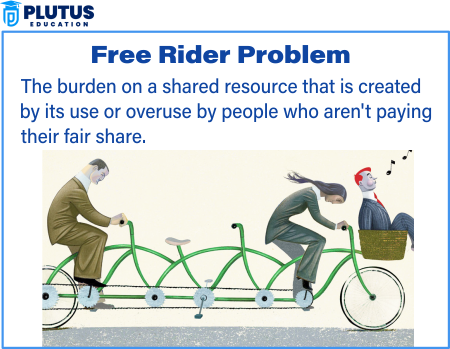
\includegraphics[width=0.65\linewidth]{BSZ_kap_12_2026/by_slide/slide_012/BSZ_kap_12_2026_slide_012_asset_01_image3.png}
  \caption{Trade-off mellom benefits og costs av desentralisering. Optimal $D^* = (B-A)/2C$. (BSZ kap.\ 12, slide 12) [SLIDE]}
\end{figure}

\begin{center}
\renewcommand{\arraystretch}{1.15}
\begin{tabular}{@{}p{3.7cm}p{4.4cm}p{5.4cm}@{}}
\toprule
\textbf{Driver} & \textbf{Trekker mot} & \textbf{Eksempel} \\
\midrule
Spesifik viden lokalt & Desentralisering & Lokal butikkpris (AutoMart) \\
Eksternaliteter mellom enheter & Sentralisering & Merkevare, IT, M\&A \\
Skalafordeler & Sentralisering & Innkjøp, treasury \\
Agentkostnader & Sentralisering & Når S2/S3 svake \\
Hastighet / lokal tilpasning & Desentralisering & Markeder med rask endring \\
Residual claimant lokalt & Desentralisering & Franchise \\
\bottomrule
\end{tabular}
\end{center}

\subsection*{Eksempler}
\begin{itemize}
\item \textbf{AutoMart (slide-eksempel):} Hvem skal sette pris -- CEO, regionsjef eller butikksjef? Lokal viden om kundepreferanser og konkurrenter ligger lokalt $\Rightarrow$ desentraliser til butikksjef, men sentraliser merkevaren og prislister-ramme. [SLIDE]
\item \textbf{Equinor E\&P:} Letevirksomhet desentralisert til prosjektledere (geologisk spesifikk viden), men store CAPEX-investeringer ratifiseres av styret (eksternalitet mot konsernrisiko, kapitalmarkedssignal). [EKS]
\item \textbf{Norsk Hydro -- pris vs.\ M\&A:} Pris på aluminium settes ikke lokalt (LME-marked), men teknologivalg på det enkelte smelteverk er desentralisert til verksledelse. M\&A-beslutninger ligger sentralt -- eksternaliteter for hele konsernet. [EKS]
\item \textbf{IKEA -- franchising vs.\ design:} Salgsbeslutninger desentralisert til varehus / franchisetaker (lokal viden). Design og produktkatalog er sentralisert i Älmhult (kodifiserbar viden + merkevareeksternalitet). [EKS]
\item \textbf{Spotify -- ``Squad model'':} Eksperiment med radikal desentralisering til autonome team. Senere delvis re-sentralisert -- viste at koordinasjonskostnader og eksternaliteter ble undervurdert. [EKS]
\item \textbf{Mærsk PtX-divisjonen:} Teknologi- og partnervalg desentralisert (spesifikk kjemisk viden), pricing av grønt drivstoff har store eksternaliteter mot Ocean-divisjonen $\Rightarrow$ koordinert; CAPEX over terskel ratifiseres sentralt. Klassisk balanseskap. [CASE]
\end{itemize}

\subsection*{Kobling til søyle og andre teorier}
Søyle: \SOne\ definisjonelt -- dette \emph{er} S1. Driver \STwo\ (måltall som speiler den allokerte beslutningen, jf.\ \thref{controllability-principle}{controllability}) og \SThree\ (insentiver på det som er allokert). Relaterte: \thref{specific-vs-general-knowledge}{Spesifik vs.\ generell viden} (kjernedriver), \thref{centralization-vs-decentralization}{Centralisering vs.\ desentralisering} (graden), \thref{decision-management-control}{Decision Management vs.\ Decision Control} (separasjon innen S1), \thref{externalities}{Eksternaliteter} (begrenser desentralisering), \thref{residual-claimants}{Residual claimants} (sentral for Control-allokering), \thref{agency-costs}{Agentomkostninger}, \thref{principal-agent}{Principal-agent}, \thref{moral-hazard}{Moral hazard}, \thref{responsibility-centers}{Responsibility centers} (implementering), \thref{organizational-architecture}{Organizational architecture} (helheten).

\paragraph{Brukt i spørsmål:} Q07.

% Q08 theories
% !TEX root = ../main.tex
\section{Reservation utility}\label{thr:reservation-utility}

\paragraph{Definisjon.} \emph{Reservation utility} ($U_0$) er det minimumsnyttenivået en (potensiell) ansatt krever for å akseptere -- eller bli værende i -- en stilling. Den tilsvarer nytten av neste-beste alternativ, og fungerer som \emph{participation constraint} i alle kontraktsdesignproblemer: en kontrakt blir bare signert (eller ikke sagt opp) hvis den gir minst $U_0$. [SLIDE]

\subsection*{Forklaring}

Reservation utility er gulvet i kompensasjonsdesign. Bedriften har én førsteoppgave: \emph{tiltrekke} og \emph{retentere} medarbeidere -- og det krever at den totale ``nyttepakken'' (lønn + fringe + ikke-monetære goder + karrierevei + status + arbeidsmiljø) ligger over kandidatens reservation utility. Reservation utility er ikke et absolutt nivå; det varierer med konjunktur, geografi, alternative arbeidsgivere, individuelle preferanser, dual-career hensyn, ikke-monetære faktorer og medarbeiderens generell og spesifik viden (jf.\ \thref{specific-vs-general-knowledge}{spesifik vs.\ generell viden}). [SLIDE]

Formelt brukes $U_0$ som bibetingelse i bedriftens kostnadsminimering: bedriften minimerer kompensasjonskostnaden $C(S,F,\ldots)$ for å levere en pakke som tilfredsstiller $U(\text{pakke}) \geq U_0$. Reservation utility er dermed både det \emph{økonomiske gulvet} for kontrakten og koblingen mellom arbeidsmarkedet ute og kompensasjonsdesignet inne. [SLIDE/BOK]

\subsection*{Determinanter av reservation utility}
\begin{itemize}
\item \textbf{Neste-beste lønnsalternativ.} For en kandidat med generell viden er $U_0$ tett bundet til markedslønnen for ekvivalente stillinger.
\item \textbf{Ikke-monetære faktorer.} Geografi, pendletid, work-life balance, arbeidsmiljø, status, autonomi, mening og karriereutsikter.
\item \textbf{Individuelle forhold.} Familie- og dual-career hensyn, helse, mobilitet, risikoaversjon.
\item \textbf{Markedet for talent.} Konjunktur, etterspørsel etter spesifik kompetanse, antall konkurrerende arbeidsgivere.
\item \textbf{Søkekostnader.} Friksjonen ved å finne neste jobb hever inkumbent-arbeidsgivers handlingsrom over $U_0$.
\item \textbf{Switching cost / firmaspesifikk humankapital.} Investert spesifik humankapital som ikke kan overføres, demper $U_0$ for retention (men ikke for første ansettelse).
\end{itemize}

\subsection*{Kjerneforutsetninger}
\begin{itemize}
\item Den ansatte har et reservasjonsnivå som er identifiserbart (selv om det er privat informasjon -- jf.\ \thref{adverse-selection}{adverse selection}).
\item Nytte er monotont stigende i lønnskomponentene -- pakker kan rangeres.
\item Det finnes et alternativ -- en outside option -- som forankrer $U_0$.
\item Kandidaten er rasjonell og sammenligner nåverdier (medregnet karriereutsikter, pensjon, jobbsikkerhet).
\end{itemize}

\subsection*{Muligheter}
\begin{itemize}
\item Forklarer hvorfor bedrifter må overstige markedet for å rekruttere knappe profiler.
\item Gir formelt grunnlag for participation constraint i \thref{principal-agent}{prinsipal--agent}-modeller (Holmström 1979): kontrakt $w(\pi)$ må gi $E[u(w)] - c(e) \geq U_0$.
\item Forklarer hvorfor bedrifter i lavpressmarkeder kan presse marginen ned og hvorfor i pressmarkeder må betale mer (eller flytte mix mot fringe).
\item Kobler arbeidsmarkedets ytre konkurranse til interne lønnssystemer og fringe-design.
\end{itemize}

\subsection*{Begrensninger og kritikk}
\begin{itemize}
\item \textbf{Privat informasjon.} $U_0$ er skjult informasjon -- bedriften observerer den ikke. Dette åpner for \thref{adverse-selection}{adverse selection} (overdrivelse av outside option) og forhandlingsasymmetri.
\item \textbf{Endogenitet.} $U_0$ kan endre seg med bedriftens egen oppførsel -- en sterk merkevare og kultur senker andres $U_0$ men hever den hos egne ansatte.
\item \textbf{Reference dependence / loss aversion.} Ansatte sammenligner ikke bare med outside option, men også med kolleger og tidligere lønn (Kahneman/Tversky). Statisk $U_0$ ignorerer dette.
\item \textbf{Ikke-monetær diskontering varierer.} Reservation utility er multidimensjonal -- vanskelig å redusere til ett tall ved heterogene preferanser.
\item \textbf{Sosiale normer og fairness.} Lønn under opplevd fair-nivå senker innsats selv om $U_0$ er møtt -- jf.\ Akerlofs gift-exchange og efficiency wages.
\item \textbf{Dynamikk:} $U_0$ stiger over tid med erfaring og humankapital -- bedrifter kan miste folk de tidligere kunne beholde.
\end{itemize}

\subsection*{Modell / illustrasjon}

\begin{figure}[H]
  \centering
  
\includegraphics[width=0.55\linewidth]{BSZ_kap_14_2026/by_slide/slide_002/BSZ_kap_14_2026_slide_002_asset_01_image1.jpeg}
  \caption{``I don't get out of bed for less than \$10,000 a day'' -- Linda Evangelista. Reservation utility i praksis: kandidaten har et minimum som må overstiges. (BSZ kap.\ 14, slide 2) [SLIDE]}
\end{figure}

Bedriftens problem:
\[
  \min_{S,F} \; C(S,F) \qquad \text{s.t.} \qquad U(S,F) \;\geq\; U_0 .
\]
$U_0$ er den indifferenskurven i $(S,F)$-planet som kontraktstilbudet \emph{minst} må berøre for å bli akseptert (se \thref{salary-fringe-benefits-mix}{salary--fringe-modellen}). Lavere $U_0$ flytter kurven inn mot origo $\Rightarrow$ billigere pakke; høyere $U_0$ flytter den utover $\Rightarrow$ dyrere. [SLIDE]

\subsection*{Eksempler}
\begin{itemize}
\item \textbf{Equinor vs.\ Aker BP (norsk olje- og energi).} Reservation utility for en petroleumsingeniør i Stavanger settes i praksis av Aker BP / ConocoPhillips. Equinor må overstige denne -- og bruker kombinasjon av høy grunnlønn, langsiktig opsjonsprogram og bred karrierevei på tvers av olje/fornybar. [EKS]
\item \textbf{Norsk offentlig sektor vs.\ konsulentbransjen.} Sykepleier med generell utdanning har $U_0$ satt av offentlige tariffer; bytter sjelden til privat fordi pensjon og jobbsikkerhet hever ``pakkenytten'' over tilsynelatende høyere private lønninger. En konsulent i BCG/McKinsey har $U_0$ definert av investment banking og tech -- høyt og stigende. [EKS]
\item \textbf{Mærsk Power-to-X.} Reservation utility for en elektrolyse-ingeniør i København defineres av Ørsted (hjemmemarkedet) og Siemens Energy / Topsoe (internasjonalt). PtX-divisjonen må enten matche pengepakke eller vri mix mot fringe og karrierevei. [CASE]
\item \textbf{Geografisk mobilitet.} Stilling i avsidesliggende lokasjon (offshore-anlegg, gruvedrift) har høyere $U_0$ for kandidater med familie $\Rightarrow$ \thref{compensating-differentials}{compensating differential} må betales på toppen. [EKS]
\end{itemize}

\subsection*{Kobling til søyle og andre teorier}
Søyle: primært \SThree\ (insentivstrukturer / kompensasjon), med koblinger til \SOne\ (hvem som tildeles roller) og \STwo\ (prestasjonskobling). Reservation utility er \emph{participation constraint} i \thref{principal-agent}{prinsipal--agent}-modellen; den setter rammen for \thref{compensating-differentials}{compensating differentials}; den tangerer \thref{salary-fringe-benefits-mix}{salary--fringe-mixen} og forklarer hvorfor \thref{superior-assets}{superior assets} gir bedriften fordel ved at den kan levere $U_0$ rimeligere enn konkurrenten. Relatert til \thref{adverse-selection}{adverse selection} (privat informasjon om $U_0$), \thref{moral-hazard}{moral hazard} (incentive constraint kommer i tillegg) og \thref{agency-costs}{agency costs}.

\paragraph{Brukt i spørsmål:} Q08, Q15.

% !TEX root = ../main.tex
\section{Compensating differentials}\label{thr:compensating-differentials}

\paragraph{Definisjon.} \emph{Compensating wage differentials} er den tilleggslønnen (eller andre kompenserende fordeler) bedriften må betale for at en ansatt skal akseptere en jobb med uattraktive trekk -- for eksempel høy risiko, nattskift, isolert lokasjon, stress eller dårlig arbeidsmiljø. Begrepet stammer fra Adam Smith (\emph{Wealth of Nations}, 1776) og er det empiriske utgangspunktet for hedoniske lønnsmodeller. [SLIDE/BOK]

\subsection*{Forklaring}

Når jobber er heterogene -- ulike i risiko, arbeidstid, lokasjon, status, mening -- må arbeidsmarkedet i likevekt kompensere arbeidstakeren for de \emph{disutility}-skapende trekkene. Hvis to ellers identiske jobber tilbys i konkurransemarked, men den ene innebærer en livsfare- eller skiftulempe, må den jobben tilby høyere lønn (eller bedre andre vilkår) for å fylles. Lønnsforskjellen kompenserer akkurat for ulempen ved marginen -- og avhenger av hvor stor andel av arbeidstilbudet som har lav aversjon mot trekket. [SLIDE]

Compensating differentials er nært knyttet til \thref{reservation-utility}{reservation utility}: $U_0$ \emph{stiger} for jobber med uattraktive trekk, og bedriften må enten heve lønnen $S$, øke fringe $F$, eller fjerne det uattraktive trekket. Hedonisk lønnsteori (Rosen 1974) operasjonaliserer dette som et likevektsproblem der lønnen er en funksjon av jobbattributter, og arbeidstakere med ulike preferanser sorteres til ulike jobber via markedet. [BOK]

\subsection*{Eksempler på uattraktive jobbtrekk}
\begin{itemize}
\item Fysisk risiko (offshore, gruvedrift, bygg, brannvesen).
\item Nattskift og skiftarbeid (sykepleiere, prosessindustri, varehus).
\item Geografisk avsidesliggende lokasjon (oljeplattform, gruve, anleggsleir).
\item Stress og høy psykisk belastning (akuttmottak, traders, militær innsats).
\item Lavt sosial status eller stigma (avfallshåndtering, slakteri).
\item Lange perioder borte fra familie (sjøfart, internasjonal konsulent).
\end{itemize}

\subsection*{Kjerneforutsetninger}
\begin{itemize}
\item \textbf{Konkurransemarked} (eller minst flerlets utstrekning av valgmuligheter). I monopsoni får arbeidstaker ikke full kompensasjon.
\item \textbf{Informasjon om jobbtrekkene} er rimelig tilgjengelig før kontrakt signeres.
\item \textbf{Heterogene preferanser:} Noen ansatte verdsetter trekk som andre disliker (en sjøfarer kan elske livet på dekk).
\item \textbf{Mobilitet:} Arbeidstakere kan velge mellom jobber; ingen friksjon hindrer sortering.
\item \textbf{Substitusjon mulig mellom lønn og jobbtrekk} (eller mellom lønn og fringe som demper trekket).
\end{itemize}

\subsection*{Muligheter}
\begin{itemize}
\item Forklarer hvorfor offshore-ingeniører tjener mer enn onshore-kolleger med samme utdanning og erfaring.
\item Operasjonaliserer ``risikoens pris'' -- statistical value of life (VSL) er estimert via differentials.
\item Forklarer hvorfor mindre attraktive lokasjoner må tilby ``hardship allowance'' eller fly inn-fly ut-rotasjoner.
\item Forklarer hvorfor sykepleiere på natt har tillegg, og hvorfor brannmenn og politi har tidlig pensjon.
\item Gir grunnlag for sortering: ansatte med lav aversjon mot trekket tar jobben billigere $\Rightarrow$ effisient matching.
\end{itemize}

\subsection*{Begrensninger og kritikk}
\begin{itemize}
\item \textbf{Empirisk vanskelig å isolere.} Lønnsforskjeller skyldes også humankapital, sortering og lokalmarkedsforhold; rene compensating differentials er notorisk vanskelige å måle (Hwang/Mortensen/Reed 1998).
\item \textbf{Forutsetter informert valg.} Ved skjult risiko (asbest, fremtidige helseplager) får arbeidstakeren \emph{ex ante} ikke full kompensasjon.
\item \textbf{Monopsoni og friksjoner.} I tynne arbeidsmarkeder kan bedriften betale under compensating-nivået fordi alternativene mangler.
\item \textbf{Heterogene preferanser kompliserer.} Markedslønnen reflekterer marginal-arbeidstakerens preferanser; inframarginale ansatte får ``konsumentoverskudd''.
\item \textbf{Sosiale normer:} Risikofylte jobber utført av migrant- eller utsatt arbeidskraft betales ofte under teoretisk compensating-nivå -- markedet fungerer ikke perfekt.
\item \textbf{Substitusjon ikke alltid mulig:} Noen jobbtrekk (livstid på rigg) er ikke direkte byttbare mot lønn; det er en nytteterskel.
\item \textbf{Kobler dårlig på psykologiske faktorer:} Mening, identitet, kall -- folk kan velge ``ukompensert'' utfordrende arbeid (sykepleier, lærer, militær) som teorien forklarer dårlig.
\end{itemize}

\subsection*{Modell / illustrasjon}

\begin{figure}[H]
  \centering
  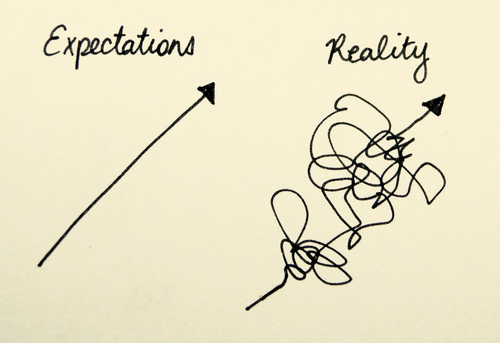
\includegraphics[width=0.55\linewidth]{BSZ_kap_14_2026/by_slide/slide_003/BSZ_kap_14_2026_slide_003_asset_01_image2.jpeg}
  \caption{Expectations vs.\ Reality -- compensating differentials kompenserer for gapet mellom forventninger og faktiske jobbforhold. (BSZ kap.\ 14, slide 3) [SLIDE]}
\end{figure}

I et lønns--risikodiagram (lønn $w$ på y-aksen, jobbrisiko $r$ på x-aksen) krysser arbeidstakerens indifferenskurver (stigende -- mer risiko krever mer lønn) bedriftens iso-profittkurver (stigende -- bedriften vil heller redusere risiko enn betale mer). I likevekt: tangering. Markedet aggregerer disse til en hedonisk lønnskurve $w^*(r)$ som er stigende i $r$. Compensating differential = $\partial w^* / \partial r > 0$. [BOK]

\subsection*{Eksempler}
\begin{itemize}
\item \textbf{Norsk sokkel -- offshore-tillegg.} Equinor og Aker BP betaler 30--40\% høyere lønn pluss skiftrotasjon (2-3-4) for arbeid på plattform vs.\ landorganisasjon -- compensating differential for isolering, risiko og borte-fra-familie. [EKS]
\item \textbf{Sykepleiere -- nattillegg.} Tariffert nattillegg + helligdagstillegg er klassisk compensating differential for skiftarbeidets disutility. [EKS]
\item \textbf{Mærsk Power-to-X -- remote anlegg.} Storskala elektrolyseanlegg lokaliseres ofte i avsidesliggende industriområder (havvindkobling, areal, infrastruktur). PtX må kompensere for lokasjon -- enten via lønn, fly-in/fly-out, midlertidig bolig eller home-office-vilkår. [CASE]
\item \textbf{Investment banking vs.\ corporate finance.} 80-timers uker i M\&A betales med høy bonus -- compensating differential for arbeidsbelastning og work-life-balance. [EKS]
\item \textbf{Antarktis-forskningsstasjon.} Britiske BAS og norske Troll-stasjonen betaler isolasjonstillegg + lang vinterbonus. [EKS]
\end{itemize}

\subsection*{Kobling til søyle og andre teorier}
Søyle: primært \SThree\ (kompensasjon), med kobling til hvem som tar hvilke roller. Compensating differentials hever \thref{reservation-utility}{reservation utility} for jobber med uattraktive trekk. Henger sammen med \thref{salary-fringe-benefits-mix}{salary--fringe-mixen}: ulempe kan kompenseres med lønn, men også med fringe (ekstra ferie, helseforsikring, hjemreiser) -- og valget styres av bedriftens kostnadsstruktur og ansattes preferanser. Kobles til \thref{superior-assets}{superior assets} -- en bedrift med sterk merkevare eller mening kan redusere det effective ``ulempe-nivået'' og dermed sin compensating-utgift. Relatert til \thref{adverse-selection}{adverse selection} (risikoinformasjon).

\paragraph{Brukt i spørsmål:} Q08.

% !TEX root = ../main.tex
\section{Superior assets (firm-specific assets)}\label{thr:superior-assets}

\paragraph{Definisjon.} \emph{Superior assets} er firmaspesifikke ressurser, organisatoriske egenskaper eller komplementaritets-strukturer som gjør at bedriften kan levere en gitt ``pakke-nytte'' til en ansatt \emph{billigere} enn konkurrenten kan -- eller en høyere ``pakke-nytte'' for samme kostnad. Eksempler er sterk merkevare, omdømme som arbeidsgiver, internt arbeidsmarked og karriereveier, organisasjonskultur, kompetansemiljø, skalaeffekter på forsikringer, og skattefavoriserte fringe-strukturer. [SLIDE/BOK]

\subsection*{Forklaring}

To bedrifter som konkurrerer om samme talent har samme \thref{reservation-utility}{reservation utility} ($U_0$) å overstige. Hvis A og B er identiske, må de tilby samme kostnad for å lande kandidaten. Men hvis A har en \emph{superior asset} -- en kapabilitet konkurrenten ikke har, eller har på dårligere vilkår -- kan A levere $U_0$ til lavere kostnad. Det gir A en strukturell konkurransefordel i arbeidsmarkedet uten å undergrave kandidatens egen nytte. [SLIDE]

Mekanikken: i $(S,F)$-planet (se \thref{salary-fringe-benefits-mix}{salary--fringe-modellen}) flytter superior asset A's isokostnadslinje innover for et gitt nivå av sammensatt kompensasjon. A når kandidatens indifferenskurve $U_0$ ved et punkt nærmere origo (lavere total kostnad) enn B. Alternativt: ved samme budsjett kan A tilby en pakke som ligger på en høyere indifferenskurve enn B. [SLIDE/BOK]

\subsection*{Typiske kilder til superior assets}
\begin{itemize}
\item \textbf{Organisatorisk omdømme / employer brand.} Google, McKinsey, Mærsk -- prestisje senker det monetære beløpet kandidaten krever.
\item \textbf{Internt arbeidsmarked og karrierevei.} Lange karrierestiger, internasjonale rotasjoner, lederopplæring -- gjør $U_0$ rimeligere å oppfylle med ikke-monetær fremtidsverdi.
\item \textbf{Kultur og mening.} IKEA-\emph{vägen}, Patagonias miljøetos, Mærsks maritime tradisjon -- folk vil jobbe der \emph{billigere} fordi det er meningsfullt.
\item \textbf{Skattefordel på fringe.} Bedriftens kostnad for $1$ NOK pensjon kan være lavere enn $1$ NOK lønn (skatt og avgift forskjellig). Den ansatte verdsetter pensjonens kontantekvivalent høyere enn bedriftens kostnad.
\item \textbf{Kvantumsrabatt / skala.} Stor bedrift kjøper helseforsikring, treningsabonnementer eller kantine billigere per ansatt enn små.
\item \textbf{Komplementært kompetansemiljø.} Novo Nordisks forskningsmiljø; en farmasøyt får mer fagutvikling der enn alene hos en konkurrent.
\item \textbf{Lokaliserings- og infrastrukturfordel.} Hovedkontor med kantine, barnehage, gym, transportordning -- bedriften tilbyr disse til en kostnad konkurrenten på avstand ikke kan.
\item \textbf{Eiermodell / langsiktighet.} Stiftelses- eller familieeid bedrift kan tilby langsiktig jobbsikkerhet som en outside-option-bedrift ikke kan signalere troverdig.
\end{itemize}

\subsection*{Kjerneforutsetninger}
\begin{itemize}
\item Bedriften har en \emph{asymmetrisk fordel} på en eller flere kompensasjonsdimensjoner.
\item Fordelen er \emph{vanskelig å imitere} -- ellers konkurrerer den bort.
\item Den ansatte verdsetter fordelen (preferanser må stemme overens).
\item Substitusjon mellom lønn og asset-leverte goder er mulig i ansattes nytte.
\item Asset kan opprettholdes uten å undergrave seg selv (kultur fortynnes når man vokser for fort -- en grenseproblem).
\end{itemize}

\subsection*{Muligheter}
\begin{itemize}
\item Forklarer hvorfor noen bedrifter konsistent kan rekruttere knapt talent uten å betale markedstopp -- de leverer pakkenytte rimeligere.
\item Begrunner investering i kultur, employer brand, læringsmiljø, on-site goder.
\item Operasjonaliserer Resource-Based View (Barney 1991) i arbeidsmarkedet: VRIN-egenskaper (valuable, rare, inimitable, non-substitutable) hos selve organisasjonen.
\item Forklarer hvorfor lønnsmix varierer på tvers av bransjer: superior asset på fringe-siden (pensjon, helseforsikring) i bedrifter med stordriftsfordel; superior asset på lønnsiden i bedrifter uten.
\item Forklarer hvorfor nystartede selskaper må betale mer i kontant lønn for å lande samme talent som etablerte aktører.
\end{itemize}

\subsection*{Begrensninger og kritikk}
\begin{itemize}
\item \textbf{Asset kan forvitre.} Omdømme tar lang tid å bygge og kan ødelegges fort (skandaler, oppsigelsesrunder). Den superior-egenskapen er ikke statisk.
\item \textbf{Heterogene preferanser.} En kulturasset verdsettes ulikt -- en ansatt som ikke deler verdiene vil ikke ``betale'' lavere lønn for å være der.
\item \textbf{Sortering kan låse selskapet.} Sterk kultur tiltrekker likesinnede; mister diversitet og er sårbar når omgivelser endrer seg.
\item \textbf{Måleproblem.} Verdien av superior asset er vanskelig å kvantifisere; lederen kan over- eller undervurdere den.
\item \textbf{Konkurrenter imiterer.} Synlige fordeler (gratis lunsj, gym) kopieres lett; \emph{bare} ikke-imiterbare assets gir varig fordel.
\item \textbf{Kan utnyttes opportunistisk:} Bedriften kan utvanne lønn fordi ``vi har kultur'' -- men hvis kulturen ikke leverer reell nytte til den ansatte, kollapser modellen.
\item \textbf{Skattefavør kan endres.} Politiske endringer fjerner én av de viktigste superior-assets på fringe-siden.
\end{itemize}

\subsection*{Modell / illustrasjon}

\begin{figure}[H]
  \centering
  
\includegraphics[width=0.45\linewidth]{BSZ_kap_8_2026/by_slide/slide_009/BSZ_kap_8_2026_slide_009_asset_01_image4.jpeg}
  \caption{Superior assets: Cristiano Ronaldo som eksempel -- firmaspesifikke ressurser som skaper verdi utover det som kan kjøpes i markedet. (BSZ kap.\ 8, slide 9) [SLIDE]}
\end{figure}

I $(S,F)$-planet: konkurrenten B har isokostnadslinje $c_S^B \cdot S + c_F^B \cdot F = K^B$. Bedrift A har superior asset på $F$ -- den kjøper helseforsikring 30\% billigere $\Rightarrow$ $c_F^A < c_F^B$. A's isokostnadslinje er \emph{flatere} (samme $K$ kjøper mer $F$). A når kandidatens indifferenskurve $U_0$ ved et punkt med mer $F$ og mindre $S$ -- og lavere total kostnad. Tangering forklart i \thref{salary-fringe-benefits-mix}{salary--fringe-modellen}. [SLIDE]

\subsection*{Eksempler}
\begin{itemize}
\item \textbf{Novo Nordisk.} Skandinaviens fremste diabetes-forskningsmiljø $\Rightarrow$ en farmasøyt eller bioingeniør får faglig utvikling og publikasjonsmuligheter andre selskaper ikke kan matche. Lønnen kan ligge under amerikanske Big Pharma uten å tape rekrutteringskamp. [EKS]
\item \textbf{Equinor.} Stor karrierevei på tvers av olje, gass, fornybar, internasjonalt + omfattende pensjonsordning gjennom Statens pensjonskasse-aktige strukturer -- pakke en mindre, ung fornybarutfordrer (f.eks.\ Scatec) ikke kan tilby. [EKS]
\item \textbf{IKEA.} ``IKEA-vägen'' -- kultur, internopplæring i Älmhult, lange karrierer fra varehus til ledelse $\Rightarrow$ varehussjefer rekrutteres internt billigere enn konkurrenten kan rekruttere eksternt. [EKS]
\item \textbf{Google / Alphabet.} On-site gratis mat, gym, transport, plus aksjeprogrammer -- skalafordel på fringe gjør pakkenytten høy ved lavere marginalkostnad enn små selskaper. [EKS]
\item \textbf{Mærsk Power-to-X.} A.P.\ Møller-Mærsk-stiftelsens langsiktige eierskap signaliserer jobbsikkerhet og strategisk forankring; København-HQ med velferdsgoder; kryss-divisjon karrierevei (shipping $\to$ logistikk $\to$ PtX $\to$ Maersk Energy). Konkurrenten Ørsted har sin egen sterke superior asset (renomme i havvind), Siemens Energy har global skala -- ulike assets gir ulike optimale lønnsmixer. [CASE]
\end{itemize}

\subsection*{Kobling til søyle og andre teorier}
Søyle: \SOne\ (allokering av roller -- karrierevei er superior asset) og \SThree\ (kompensasjon -- bedriften kan vri mix billigere). Superior assets gjør \thref{reservation-utility}{reservation utility} \emph{lettere} å oppfylle ved at bedriftens isokostnadslinje skifter favorabelt i \thref{salary-fringe-benefits-mix}{salary--fringe-modellen}. Dette demper også behovet for \thref{compensating-differentials}{compensating differentials} -- en sterk arbeidsgivermerkevare gjør at ansatte aksepterer uattraktive trekk for mindre tillegg. Kobles til \thref{specific-vs-general-knowledge}{spesifik vs.\ generell viden}: firmaspesifik humankapital er én form for superior asset (det binder ansatt og bedrift gjensidig).

\paragraph{Brukt i spørsmål:} Q08.

% !TEX root = ../main.tex
% NB: Denne filen bruker TikZ. Orkestrator: vennligst legg til
% \usepackage{tikz} i notes/preamble.tex hvis ikke allerede til stede.
\section{Salary vs.\ fringe benefits-modellen}\label{thr:salary-fringe-benefits-mix}

\paragraph{Definisjon.} Modellen for \emph{optimal mix mellom lønn (salary, $S$) og fringe benefits ($F$)} bestemmer hvordan bedriften skal sette sammen kompensasjonspakken slik at den ansattes \thref{reservation-utility}{reservation utility} oppfylles til lavest mulig kostnad for bedriften. Optimum oppstår der den ansattes \emph{indifferenskurve} er tangent til bedriftens \emph{isokostnadslinje}: bedriftens marginal-substitusjonsrate i kostnad er lik den ansattes marginal-substitusjonsrate i nytte. [SLIDE/BOK]

\subsection*{Forklaring}

Kompensasjon består typisk av (i) kontant lønn $S$ og (ii) fringe benefits $F$ -- pensjon, helseforsikring, firmabil, ekstra ferie, barnehageplass, lunsjordning, treningsmedlemskap, opsjoner med mer. Hvorfor ikke bare betale alt i lønn og la den ansatte velge selv?
\begin{enumerate}
\item \textbf{Skattefavør.} Mange fringe-elementer beskattes lavere enn lønn (pensjon, naturalytelser opp til grense). $1$ kr i fringe gir mer disponibel nytte enn $1$ kr i lønn $\Rightarrow$ bedriftens kostnad per nytte-enhet er lavere på $F$.
\item \textbf{Kvantumsrabatt / skala.} Bedriften får helseforsikring, abonnementer, kantine billigere per ansatt enn individet kan kjøpe alene.
\item \textbf{Superior assets.} Bedriften eier ressurser (kantine, kontorbygg, opplæringsprogram) som leverer nytte til ansatt til lav marginalkostnad -- jf.\ \thref{superior-assets}{superior assets}.
\item \textbf{Imperfekte substitutter.} Ansatte verdsetter $S$ og $F$ ulikt, og marginalmaten er fallende i hver komponent $\Rightarrow$ indifferenskurver er konvekse.
\end{enumerate}
[SLIDE]

\subsection*{Det formelle problemet}

Bedriften minimerer kostnaden $C(S,F) = c_S \cdot S + c_F \cdot F$ med bibetingelsen at den ansatte minst når reservation utility:
\[
  \min_{S,F} \; c_S \, S + c_F \, F \qquad \text{s.t.} \qquad U(S,F) \;\geq\; U_0 .
\]
Her er $c_S$ bedriftens marginalkostnad per krone lønn (typisk $> 1$ grunnet arbeidsgiveravgift, feriepenger, pensjon-på-pensjon), og $c_F$ er bedriftens marginalkostnad per nytte-enhet fringe. Hvis $c_F < c_S$ -- typisk pga.\ skatt eller skala -- gjøres det \emph{billigere} for bedriften å levere nytte via $F$ enn $S$. [BOK]

\paragraph{First-order condition.} I optimum gjelder
\[
  \mathrm{MRS}_{S,F} \;=\; \frac{\partial U / \partial S}{\partial U / \partial F} \;=\; \frac{c_S}{c_F}.
\]
Den ansattes vilje til å gi opp fringe for én ekstra krone lønn skal være lik bedriftens kostnadsforhold mellom de to. Geometrisk: tangering i $(S,F)$-planet mellom indifferenskurve $U_0$ og isokostnadslinje.

\subsection*{Modell / graf}

\begin{figure}[h]
  \centering
  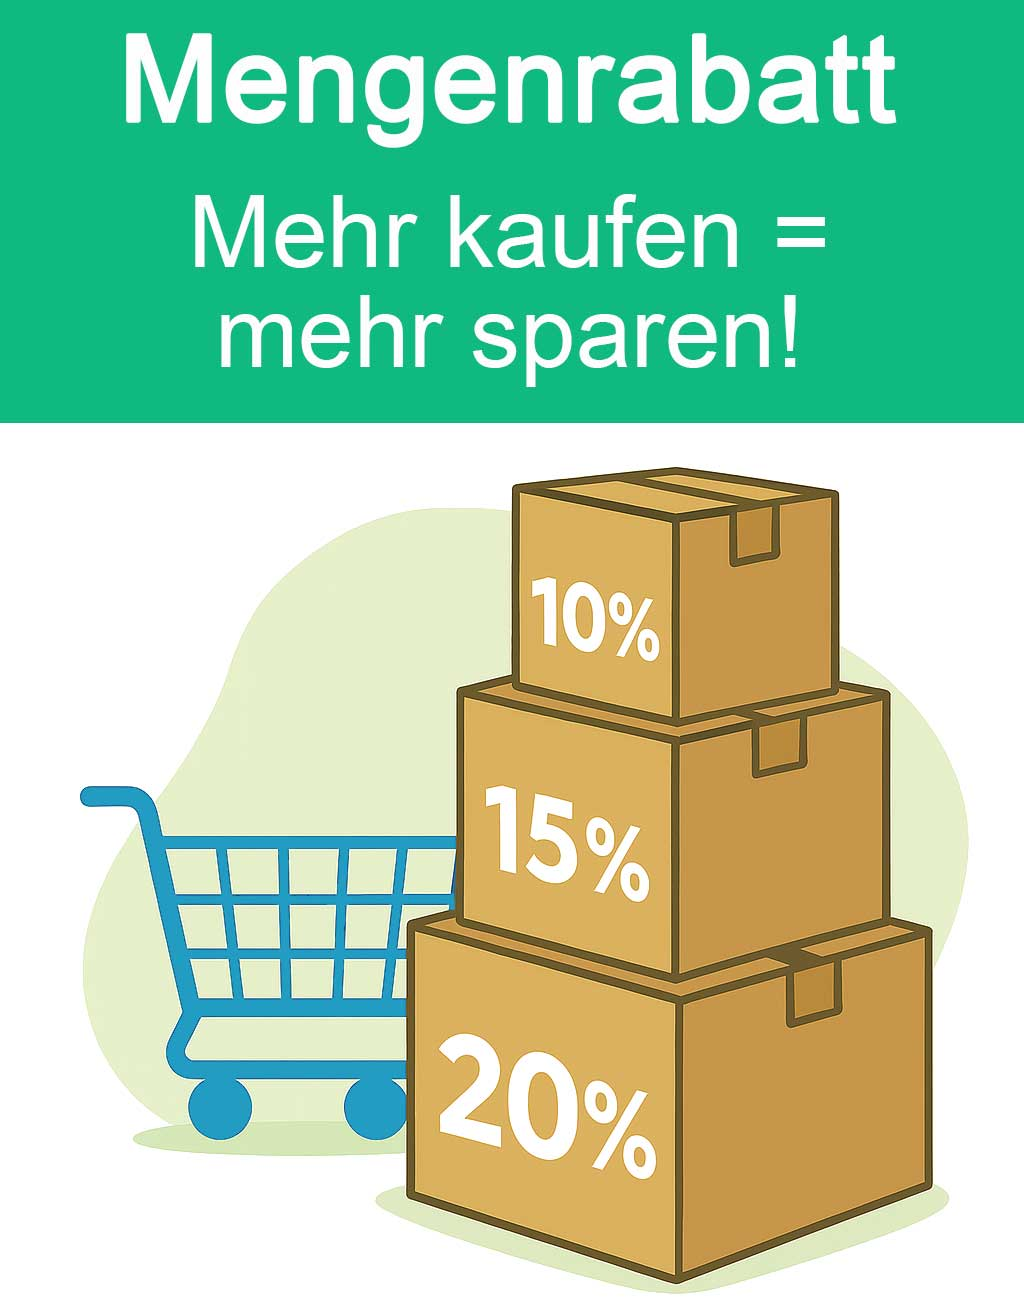
\includegraphics[width=0.35\linewidth]{BSZ_kap_14_2026/by_slide/slide_014/BSZ_kap_14_2026_slide_014_asset_01_image5.jpeg}
  \caption{Mengenrabatt: ``Mehr kaufen = mehr sparen'' -- kvantumsrabatter gjør fringe benefits billigere per enhet enn individuelt kjøp. (BSZ kap.\ 14, slide 14) [SLIDE]}
\end{figure}

\begin{figure}[h]
  \centering
  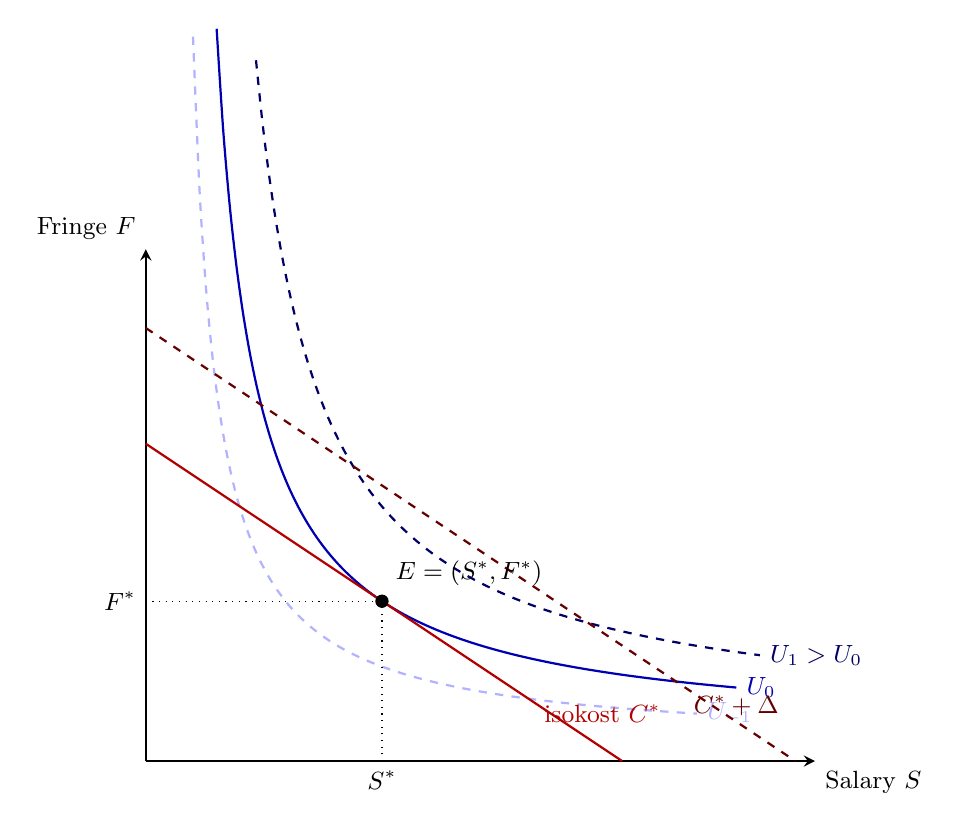
\begin{tikzpicture}[scale=1.0, >=stealth]
    % Akser
    \draw[->, thick] (0,0) -- (8.5,0) node[below right] {\small Salary $S$};
    \draw[->, thick] (0,0) -- (0,6.5) node[above left] {\small Fringe $F$};

    % Tre indifferenskurver (konvekse, U_0 nederst, så U_1, U_2)
    % U_0 -- reservation utility (passerer gjennom optimum)
    \draw[blue!70!black, thick, domain=0.9:7.5, smooth, samples=80]
      plot (\x, {4.5/(\x-0.4) + 0.3}) node[right] {\small $U_0$};
    % U_1 -- høyere nyttenivå
    \draw[blue!40!black, thick, dashed, domain=1.4:7.8, smooth, samples=80]
      plot (\x, {6.8/(\x-0.6) + 0.4}) node[right] {\small $U_1 > U_0$};
    % U_-1 -- lavere nyttenivå (under reservation -- ikke akseptert)
    \draw[blue!30, thick, dashed, domain=0.6:7.0, smooth, samples=80]
      plot (\x, {2.7/(\x-0.3) + 0.2}) node[right] {\small $U_{-1}$};

    % Isokostnadslinjer (rette, fallende). Helning = -c_S / c_F
    % Velg tangering i (3, 2)-ish. Helning = -1/2 (c_S=1, c_F=2 -- F billigere)
    % U_0 = 4.5/(x-0.4)+0.3 ; dU/dx = -4.5/(x-0.4)^2
    % I x=3: dy/dx = -4.5/(2.6)^2 = -4.5/6.76 = -0.666
    % => velg c_S/c_F = 0.666 => helning -0.666
    % Linje gjennom (3, 4.5/2.6+0.3) = (3, 2.03)
    % Linje: y = 2.03 - 0.666(x-3) -> x-skjær: 2.03/0.666 + 3 = 6.05
    %                                y-skjær: 2.03 + 0.666*3 = 4.03
    \draw[red!70!black, thick] (0, 4.03) -- (6.05, 0) node[below] {};
    \node[red!70!black] at (5.8, 0.6) {\small isokost $C^*$};

    % En høyere isokost (svakere)
    \draw[red!40!black, thick, dashed] (0, 5.5) -- (8.25, 0);
    \node[red!40!black] at (7.5, 0.7) {\small $C^* + \Delta$};

    % Optimum-punkt
    \filldraw[black] (3, 2.03) circle (2.2pt);
    \node[anchor=south west] at (3.05, 2.1) {\small $E = (S^*, F^*)$};

    % S* og F* akse-projiseringer
    \draw[dotted] (3, 0) -- (3, 2.03);
    \draw[dotted] (0, 2.03) -- (3, 2.03);
    \node[below] at (3, 0) {\small $S^*$};
    \node[left] at (0, 2.03) {\small $F^*$};
  \end{tikzpicture}
  \caption{Optimal mix mellom lønn ($S$) og fringe benefits ($F$). Den ansattes indifferenskurver $U_{-1}, U_0, U_1$ er konvekse mot origo (imperfekte substitutter). Bedriftens isokostnadslinjer har helning $-c_S / c_F$. I optimum $E$ tangerer reservation-utility-kurven $U_0$ den laveste oppnåelige isokostnadslinjen $C^*$: $\mathrm{MRS}_{S,F} = c_S/c_F$. Lavere kostnad ($C^* - \Delta$) når ikke $U_0$; høyere kostnad ($C^* + \Delta$) er sløsing. [SLIDE]}
\end{figure}

\paragraph{Hvordan grafen flyttes av endringer.}
\begin{itemize}
\item \textbf{Skatt på lønn øker} $\Rightarrow$ $c_S$ stiger $\Rightarrow$ isokostnadslinjen blir \emph{brattere} $\Rightarrow$ tangering flytter mot mer $F$, mindre $S$.
\item \textbf{Bedriften får kvantumsrabatt på forsikring} $\Rightarrow$ $c_F$ faller $\Rightarrow$ isokost blir flatere $\Rightarrow$ mer $F$ optimal.
\item \textbf{Reservation utility stiger} (stramt arbeidsmarked) $\Rightarrow$ $U_0$ flyttes utover $\Rightarrow$ minimumskostnaden $C^*$ stiger; mixen kan endre seg avhengig av preferanser.
\item \textbf{Heterogene ansatte} $\Rightarrow$ ulike indifferenskurver $\Rightarrow$ ulik optimal mix $\Rightarrow$ rasjonale for ``cafeteria-style benefits''.
\end{itemize}

\subsection*{Kjerneforutsetninger}
\begin{itemize}
\item $S$ og $F$ er \emph{imperfekte substitutter} i ansattes nytte -- begge har positiv, men avtakende marginalnytte.
\item Ansattes nyttefunksjon er kvasi-konkav (gir konvekse indifferenskurver).
\item Bedriftens kostnadsfunksjon er lineær eller konveks i $S$ og $F$.
\item $c_S \neq c_F$ -- ellers ville mix være likegyldig (kun totalbeløpet teller).
\item Bedriften kjenner -- eller estimerer rimelig -- ansattes preferanser.
\item Reservation utility $U_0$ er bindende.
\end{itemize}

\subsection*{Muligheter}
\begin{itemize}
\item Forklarer hvorfor lønn alene aldri er optimal kompensasjon når skatt og skala favoriserer fringe.
\item Begrunner cafeteria-style benefits og fleksibel kompensasjon for å håndtere preferanseheterogenitet.
\item Operasjonaliserer hvordan bedriften kan møte $U_0$ rimeligere -- direkte konkurransefordel.
\item Forklarer empirisk variasjon i lønnsmix på tvers av bedrifter, bransjer og land.
\item Gir formelt grunnlag for design av pensjons- og helseordninger.
\end{itemize}

\subsection*{Begrensninger og kritikk}
\begin{itemize}
\item \textbf{Heterogene preferanser.} Indifferenskurven varierer mellom ansatte; én pakke passer ikke alle (men cafeteria-løsninger reduserer problemet).
\item \textbf{Signaling-effekter.} Høy lønn kan signalere status og prestasje; å konvertere lønn til fringe kan rammes som ``lavere status'' selv om kontantverdien er den samme.
\item \textbf{Reference dependence.} Ansatte sammenligner lønn med kolleger; fringe er mindre synlig. For konkurransepress kan synlig lønn virke sterkere enn faktisk nytte tilsier.
\item \textbf{Likviditetspreferanse.} Unge ansatte med boliglån verdsetter kontantlønn (lav diskontering av fremtidig pensjon) mer enn modellen antar.
\item \textbf{Skatteregimer endres.} Et fringe-tungt design som er optimalt i dag kan bli suboptimalt etter politisk skift.
\item \textbf{Måleproblemer.} Verken $U(S,F)$ eller $c_F$ er presist kjent; tangering er konseptuell.
\item \textbf{Asymmetrisk informasjon.} Ansatte kjenner egne preferanser bedre enn bedriften $\Rightarrow$ \thref{adverse-selection}{adverse selection}: bedriften vet ikke hva den enkelte verdsetter.
\item \textbf{Insentiv-effekter på fringe.} Fringe gir typisk svakere prestasjonsinsentiv enn variabel lønn -- modellen ignorerer \thref{moral-hazard}{moral hazard}.
\end{itemize}

\subsection*{Eksempler}
\begin{itemize}
\item \textbf{Equinor.} Tung pensjonsordning, helseforsikring, lange ferieavtaler -- $c_F$ lav fordi statlig pensjonsstruktur og skala. Total mix har relativt høyt $F$-innslag og moderat $S$ relativt til amerikanske oljemajors. [EKS]
\item \textbf{Konsulent / investment banking (IBM, Goldman).} Lite fringe, høy bonus -- $c_F$ ikke spesielt fordelaktig, og ansatte er typisk mobile (lav verdi av pensjon hos én arbeidsgiver). Optimal mix tipper mot $S$ og kortsiktig bonus. [EKS]
\item \textbf{Novo Nordisk.} Omfattende familiefringe (helseforsikring, barnepass) hever pakkenytten for forskere som ofte har dual-career ektefelle og barn. Skattefavør i Danmark + skala. [EKS]
\item \textbf{Norsk offentlig sektor.} Lav $S$, men sterk pensjonsordning (Statens pensjonskasse) og jobbsikkerhet -- $F$-tung pakke som leverer høy $U_0$ til lav kostnad. [EKS]
\item \textbf{Cafeteria-plan i Mærsk.} Heterogene ansatte $\Rightarrow$ ansatte velger mellom ekstra ferie, pensjon, bilordning, ekstra helseforsikring; samme totalbudsjett, høyere nytte. [CASE]
\end{itemize}

\subsection*{Kobling til søyle og andre teorier}
Søyle: primært \SThree\ (insentivstruktur / kompensasjonsdesign). Modellen tar \thref{reservation-utility}{reservation utility} som bibetingelse, justerer for \thref{compensating-differentials}{compensating differentials} (uattraktive trekk hever $U_0$), og utnytter \thref{superior-assets}{superior assets} (lav $c_F$ via skala/kultur/skatt). Knyttet til \thref{principal-agent}{prinsipal--agent} (participation constraint), \thref{specific-vs-general-knowledge}{spesifik humankapital} (firm-spesifik fringe binder ansatt) og \thref{moral-hazard}{moral hazard} (fringe vs.\ variabel lønn-trade-off).

\paragraph{Brukt i spørsmål:} Q08.

% Q09 theories
% !TEX root = ../main.tex
% NB: Denne filen bruker TikZ for to grafiske modeller (agent og prinsipal).
% Orchestrator: vennligst legg til \usepackage{tikz} i notes/preamble.tex.
\section{Optimal effort-modell (agent- og prinsipalside)}\label{thr:optimal-effort-model}

\paragraph{Definisjon.} Optimal effort-modellen er den standardiserte principal-agent-rammen fra BSZ kap.\ 15 som anviser hvordan agentens innsatsnivå $e$ og prinsipalens insentivkoeffisient $\beta$ velges optimalt under risiko og asymmetrisk informasjon. Modellen kombinerer en lineær outputfunksjon $Q=\alpha e+\mu$, en lineær kontrakt $W=W_0+\beta Q$ og en risikoavers agent, og leverer to førsteordensbetingelser -- én for agenten (effort-valg) og én for prinsipalen (kontraktsdesign). [SLIDE]

\subsection*{Forklaring}

Modellen har to aktører som tar beslutninger i sekvens. \emph{Prinsipalen} (eier/virksomhet) velger først kontraktsparametrene $(W_0,\beta)$ og kunngjør dem. \emph{Agenten} (medarbeider) velger deretter innsats $e$ for å maksimere egen forventet nytte, idet $\mu$ realiseres og lønnen $W$ utbetales. Prinsipalen forutser agentens reaksjon (\emph{backward induction}) og velger derfor $(W_0,\beta)$ med agentens beste respons innebakt. Modellen er en kanonisk illustrasjon av \thref{principal-agent}{principal-agent-teori} og er kjernen i \thref{costly-contracting}{costly contracting} (med costless contracting som referansepunkt). [SLIDE/BOK]

\textbf{Outputfunksjonen.} $Q=\alpha e+\mu$ med produktivitet $\alpha>0$, innsats $e\ge 0$ og støy $\mu\sim N(0,\sigma^{2})$. Støyen representerer alt agenten ikke kontrollerer -- råvarepris, valuta, vær, etterspørsel, kollegaers handlinger. [SLIDE]

\textbf{Kontrakten.} $W=W_0+\beta Q$ er lineær: $W_0$ er den \emph{præstationsuafhængige} (faste) lønnen og $\beta\in[0,1]$ er \emph{incitamentskoefficienten} -- den andelen av $Q$ som tilfaller agenten på marginen. Lineariteten gjør at modellen lar seg løse i lukket form og er det vanlige didaktiske valget (Holmström-Milgrom 1987 viser at lineære kontrakter er optimale i en bredere CARA-mean-variance-setting). [SLIDE/BOK]

\textbf{Agentens nyttefunksjon.} I BSZ-Ian-eksemplet skrives nytten enkelt som $U=I-e^{2}$, der innsatskostnaden er $c(e)=e^{2}$ med $c'(e)=2e$. I den fulle CARA-mean-variance-formuleringen brukes:
\[
\mathrm{CE}(W,e)\;=\;\mathbb{E}[W]-\tfrac{r}{2}\mathrm{Var}[W]-c(e),
\]
hvor $\mathrm{CE}$ er agentens \emph{sikkerhetsekvivalent}, $r>0$ er absolutt risikoaversjon (Arrow-Pratt) og $\mathrm{Var}[W]=\beta^{2}\sigma^{2}$. Termen $\tfrac{r}{2}\beta^{2}\sigma^{2}$ er agentens \emph{risikopremie} -- den må kompenseres av $W_0$ for å delta. [BOK]

\subsection*{Modell A -- Agentens side (innsatsvalg)}

Med kontrakten gitt setter agenten inn $W=W_0+\beta(\alpha e+\mu)$ og maksimerer
\[
\max_{e}\;\; W_0+\beta\alpha e\;-\;\tfrac{r}{2}\beta^{2}\sigma^{2}\;-\;c(e).
\]
Førsteordensbetingelsen (FOC) er:
\begin{equation}\label{eq:agent-foc}
\boxed{\;\beta\alpha \;=\; c'(e^{*})\;}
\end{equation}
\emph{Marginalt utbytte} av innsats ($\beta\alpha$) lik \emph{marginal innsatskostnad} ($c'(e)$).

\textbf{Numerisk eksempel (Ian/AssemCo).} Med $c(e)=e^{2}$, $\alpha=100$:
\begin{itemize}\setlength{\itemsep}{2pt}
\item $\beta\alpha=2e^{*}\Rightarrow e^{*}=50\beta$.
\item $\beta=0$ (ren fast lønn): $e^{*}=0$ -- ingen insentiv, ingen innsats.
\item $\beta=1$ (full residual claimant): $e^{*}=50$ -- first-best.
\item $\beta=0{,}5$: $e^{*}=25$.
\end{itemize}
Sentralt poeng: $W_0$ vrir ikke innsats -- den faller ut av FOC. Bare $\beta$ vrir innsats. [SLIDE]

\begin{figure}[h]
\centering
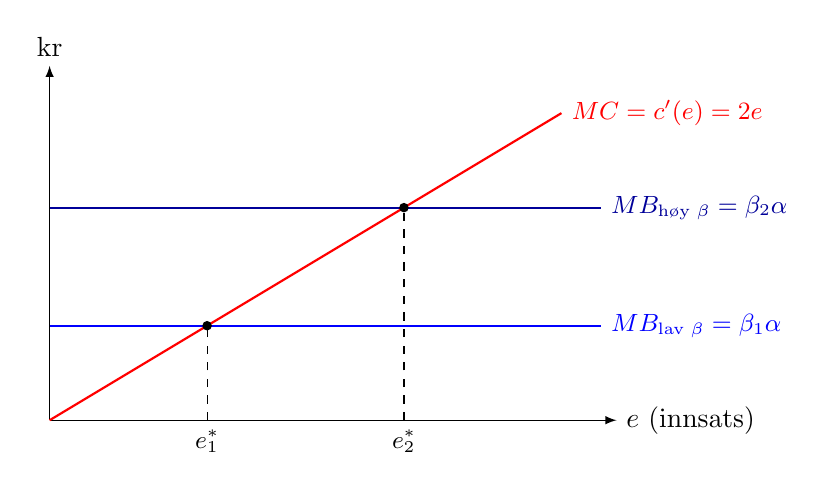
\begin{tikzpicture}[>=latex,scale=1.0]
  % Akser
  \draw[->] (0,0) -- (7.2,0) node[right] {$e$ (innsats)};
  \draw[->] (0,0) -- (0,4.5) node[above] {kr};
  % MB-linjer (konstant marginal benefit = beta*alpha)
  \draw[thick,blue] (0,1.2) -- (7,1.2) node[right] {\small $MB_{\text{lav }\beta}=\beta_1\alpha$};
  \draw[thick,blue!60!black] (0,2.7) -- (7,2.7) node[right] {\small $MB_{\text{høy }\beta}=\beta_2\alpha$};
  % MC = c'(e) = 2e (stigende)
  \draw[thick,red] (0,0) -- (6.5,3.9) node[right] {\small $MC=c'(e)=2e$};
  % Optimum 1
  \draw[dashed] (2.0,0) -- (2.0,1.2);
  \filldraw (2.0,1.2) circle (1.5pt);
  \node[below] at (2.0,0) {\small $e_1^{*}$};
  % Optimum 2
  \draw[dashed] (4.5,0) -- (4.5,2.7);
  \filldraw (4.5,2.7) circle (1.5pt);
  \node[below] at (4.5,0) {\small $e_2^{*}$};
\end{tikzpicture}
\caption{\textbf{Modell A -- agentens side.} Agenten velger $e^{*}$ der $MB=MC$, dvs.\ $\beta\alpha=c'(e)$. Når $\beta$ stiger fra $\beta_1$ til $\beta_2$, skifter $MB$ opp og optimal innsats $e^{*}$ flyttes til høyre. Fast lønn $W_0$ påvirker \emph{ikke} kurvene og dermed ikke $e^{*}$. [SLIDE -- BSZ kap.\ 15]}
\end{figure}

\subsection*{Modell B -- Prinsipalens side (optimal $\beta$)}

Prinsipalen maksimerer forventet profit $\mathbb{E}[\Pi]=\mathbb{E}[Q]-\mathbb{E}[W]$ underlagt to skranker:
\begin{itemize}\setlength{\itemsep}{1pt}
\item \emph{Incentive compatibility (IC):} agenten velger $e^{*}(\beta)$ som løser \eqref{eq:agent-foc}.
\item \emph{Participation (IR):} agentens $\mathrm{CE}\ge \overline{U}$ -- $W_0$ justeres slik at den ``binder''.
\end{itemize}
Når IR binder, ``betaler'' prinsipalen for både agentens innsatskostnad og risikopremien gjennom forventet lønn. Reduserer man problemet til valg av $\beta$, blir det:
\[
\max_{\beta}\;\;\underbrace{\alpha\,e^{*}(\beta)}_{\text{produksjonsgevinst}}\;-\;\underbrace{c\!\left(e^{*}(\beta)\right)}_{\text{innsatskostnad}}\;-\;\underbrace{\tfrac{r}{2}\beta^{2}\sigma^{2}}_{\text{risikopremie}}.
\]
Med $c(e)=e^{2}/(2k)$ slik at $c'(e)=e/k$ og dermed $e^{*}=k\beta\alpha$, blir FOC i $\beta$:
\begin{equation}\label{eq:beta-star}
\boxed{\;\beta^{*}\;=\;\dfrac{\alpha^{2}}{\alpha^{2}+r\sigma^{2}/k}\;=\;\dfrac{1}{1+r\sigma^{2}c''(e)/\alpha^{2}}\;}
\end{equation}
Dette er den klassiske Holmström-Milgrom-formelen (lineær kontrakt, CARA-nytte, normalfordelt støy). [BOK]

\textbf{Komparativ statikk.}
\begin{itemize}\setlength{\itemsep}{2pt}
\item $\beta^{*}\downarrow$ når agentens risikoaversjon $r$ stiger.
\item $\beta^{*}\downarrow$ når støyen $\sigma^{2}$ stiger -- jo mindre informativt $Q$ er om $e$, jo svakere insentiv.
\item $\beta^{*}\uparrow$ når produktiviteten $\alpha$ stiger.
\item $\beta^{*}\uparrow$ når marginalkostnaden av innsats $c''(e)$ faller (mindre konveks innsatskostnad).
\item Grensetilfeller: $r\to 0$ (risikonøytral agent) $\Rightarrow\beta^{*}\to 1$ (full residual claimancy, first-best); $\sigma^{2}\to 0$ (innsats kan ``leses ut'' av $Q$) $\Rightarrow\beta^{*}\to 1$.
\end{itemize}

\begin{figure}[h]
\centering
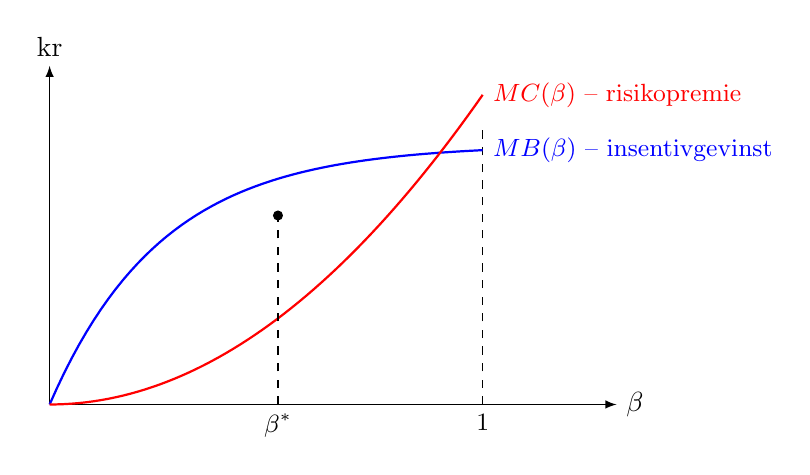
\begin{tikzpicture}[>=latex,scale=1.0]
  % Akser
  \draw[->] (0,0) -- (7.2,0) node[right] {$\beta$};
  \draw[->] (0,0) -- (0,4.3) node[above] {kr};
  \draw (5.5,0) node[below] {\small $1$};
  \draw[dashed] (5.5,0) -- (5.5,3.5);
  % Marginal benefit av β (konkav stigende): produksjonsgevinst minus innsatskostnad
  \draw[thick,blue,domain=0:5.5,samples=60]
    plot (\x,{3.3*(1-exp(-0.7*\x))}) node[right] {\small $MB(\beta)$ -- insentivgevinst};
  % Marginal cost av β (konveks stigende): risikopremie
  \draw[thick,red,domain=0:5.5,samples=60]
    plot (\x,{0.13*\x*\x}) node[right] {\small $MC(\beta)$ -- risikopremie};
  % Krysning (visuell): rundt β=2.8 i diagrammet
  \filldraw (2.9,2.4) circle (1.6pt);
  \draw[dashed] (2.9,0) -- (2.9,2.4);
  \node[below] at (2.9,0) {\small $\beta^{*}$};
\end{tikzpicture}
\caption{\textbf{Modell B -- prinsipalens side.} Prinsipalen velger $\beta^{*}$ der marginalt insentivutbytte ($MB(\beta)$, konkav stigende -- avtagende marginalgevinst av flere insentiver) lik marginal risikokostnad ($MC(\beta)$, konveks stigende -- risikopremien $\tfrac{r}{2}\beta^{2}\sigma^{2}$ stiger raskere enn lineært). $\beta^{*}<1$ i second-best; $\beta^{*}\to 1$ kun ved risikonøytral agent ($r=0$) eller perfekt observerbarhet ($\sigma^{2}=0$). [SLIDE -- BSZ kap.\ 15]}
\end{figure}

\subsection*{Slide-illustrasjon fra pensum}

\begin{figure}[h]
\centering

\includegraphics[width=0.55\linewidth]{BSZ_kap_15_2026/by_slide/slide_014/BSZ_kap_15_2026_slide_014_asset_01_image3.png}
\caption{Prinsipal-agent-modellen i BSZ kap.\ 15: $Q=\alpha e+\mu$, $W=W_0+\beta Q$, og effort-valget som funksjon av $\beta$. [SLIDE -- BSZ kap.\ 15, slide 14]}
\end{figure}

\subsection*{Kjerneforutsetninger}
\begin{itemize}\setlength{\itemsep}{1pt}
\item Lineær teknologi $Q=\alpha e+\mu$ med kjent $\alpha$ og normalfordelt $\mu$.
\item Lineær kontrakt $W=W_0+\beta Q$ (verifiserbar på $Q$).
\item CARA-nytte (eller $U=I-c(e)$) med konveks innsatskostnad $c(e)$, $c'(0)=0$, $c''(e)>0$.
\item Risikoavers agent ($r>0$), risikonøytral prinsipal (diversifisert).
\item Asymmetrisk informasjon: $e$ er ikke observerbart for prinsipalen (\thref{moral-hazard}{moral hazard}).
\item Reservasjonsnytte $\overline{U}$ utenfor virksomheten gitt (ytre arbeidsmarked).
\item Én oppgavedimensjon -- ingen multitasking (Holmström-Milgrom 1991).
\end{itemize}

\subsection*{Muligheter (hva modellen leverer)}
\begin{itemize}\setlength{\itemsep}{1pt}
\item En kvantitativ regel for hvor sterk insentivlønn skal være (\thref{incentive-coefficient}{$\beta^{*}$-formelen}).
\item En presis dekomponering av lønnen i en risikobærende og en innsatsdrivende del (\thref{fixed-vs-variable-pay}{$W_0$ vs.\ $\beta Q$}).
\item En formell forklaring på insentiv-risiko-trade-offen (\thref{risk-sharing}{risikodeling}).
\item Begrunnelsen for \thref{informativeness-principle}{informativeness-prinsippet}: redusér effektiv $\sigma^{2}$ ved bedre måltall.
\item Begrunnelsen for \thref{costly-contracting}{costly contracting}: second-best avviker fra \thref{costless-contracting}{costless contracting} nettopp pga.\ $r\sigma^{2}>0$.
\end{itemize}

\subsection*{Begrensninger og kritikk}
\begin{itemize}\setlength{\itemsep}{1pt}
\item Én-dimensjonal: i virkeligheten har agenten mange oppgaver med ulik målbarhet -- sterke insentiver på det målbare gir vridning bort fra det umålbare (Holmström-Milgrom 1991, ``equal compensation principle'').
\item Forutsetter at $Q$ er kontraktérbart -- mange resultater (kreativitet, samarbeid, kvalitet) er det ikke.
\item Risikoaversjonen $r$ og $\sigma^{2}$ må anslås -- vanskelig empirisk.
\item Ignorerer dynamikk: \emph{ratchet effect} (justert måltall år 2 dersom du leverer år 1), karriereinsentiver, reputasjon.
\item Atferdseffekter: \emph{crowding out} av indre motivasjon ved sterke ytre insentiver (Frey \& Jegen).
\item Antar én prinsipal -- multiple stakeholders (regulator, kreditorer, samfunn) bryter modellen.
\item Lineariteten er en bekvem antagelse; reelle bonusplaner har terskler, tak og opsjoner som skaper ikke-lineære insentiver og kan oppmuntre til gaming.
\item Forutsetter at agenten kjenner $\alpha$ og fordelingen av $\mu$ like godt som prinsipalen (mer realistisk: \thref{adverse-selection}{adverse selection} på begge sider).
\end{itemize}

\subsection*{Kobling til (a) risiko, (b) fast lønn, (c) $\beta$}
\begin{itemize}\setlength{\itemsep}{2pt}
\item \textbf{(a) Risiko:} Inngår i $\beta^{*}$ via $r\sigma^{2}$. Jo mer risikoavers agent og jo støyere måltall, jo lavere optimal $\beta$. Risikopremien $\tfrac{r}{2}\beta^{2}\sigma^{2}$ betales av prinsipalen gjennom forhøyet $W_0$. Se \thref{risk-sharing}{risk-sharing}.
\item \textbf{(b) Præstationsuafhængig løn $W_0$:} Faller ut av agentens FOC (vrir ikke innsats); dens rolle er å oppfylle IR-skranken og kompensere for risikopremien. Se \thref{fixed-vs-variable-pay}{fixed-vs-variable-pay}.
\item \textbf{(c) Incitamentskoefficient $\beta$:} Eneste parameter som vrir innsats. Trade-off mellom insentivgevinst og risikopremie gir formel \eqref{eq:beta-star}. Se \thref{incentive-coefficient}{incentive-coefficient}.
\end{itemize}

\subsection*{Eksempler}
\begin{itemize}\setlength{\itemsep}{2pt}
\item \textbf{Investment banking-trader:} $\sigma^{2}$ stor, men $\alpha$ også stor og trader-talenter er lite risikoaverse i porteføljen sin (har øvrig formue ofte diversifisert). Resultat: høy $\beta$, beskjeden $W_0$ -- bonuspuljen er hovedinntekten. [EKS]
\item \textbf{Offentlig sektor / lektor:} Output svært vanskelig å måle ($\sigma^{2}$ stort), agent er typisk risikoavers, og prinsipalen (stat) verdsetter likhet og normer. Resultat: $\beta\approx 0$, nesten alt $W_0$ (tarifflønn). [EKS]
\item \textbf{Selger på provisjon vs.\ butikksjef:} Selger har høyt og lett målbart $\alpha$ med relativt lite $\mu$ $\Rightarrow$ høy $\beta$. Butikksjef har bredere ansvarsområder hvor enkelte mål er mindre informative $\Rightarrow$ moderat $\beta$, betydelig $W_0$. [EKS]
\item \textbf{Equinor-CEO LTI:} Lederlønn med stor andel aksjebasert LTI, men også betydelig grunnlønn. $\sigma^{2}$ (oljepris) er stor og kompenseres delvis ved relative måltall (peer-gruppe) -- bruk av \thref{informativeness-principle}{informativeness-prinsippet}. [EKS]
\end{itemize}

\subsection*{Kobling til søyle og andre teorier}
Søyle: \STwo\ (måltallet $Q$) og \SThree\ (selve kontrakten $W_0+\beta Q$). Relaterte: \thref{principal-agent}{Principal-agent}, \thref{moral-hazard}{Moral hazard}, \thref{agency-costs}{Agency costs}, \thref{adverse-selection}{Adverse selection}, \thref{incentive-coefficient}{Incentive coefficient}, \thref{risk-sharing}{Risk sharing}, \thref{fixed-vs-variable-pay}{Fixed vs.\ variable pay}, \thref{costless-contracting}{Costless contracting}, \thref{costly-contracting}{Costly contracting}, \thref{informativeness-principle}{Informativeness-prinsippet}, \thref{specific-vs-general-knowledge}{Spesifik vs.\ generell viden} (driver fordi agenten kjenner $e$, prinsipalen ikke).

\paragraph{Brukt i spørsmål:} Q09.

% !TEX root = ../main.tex
\section{Incitamentskoefficient ($\beta$)}\label{thr:incentive-coefficient}

\paragraph{Definisjon.} \emph{Incitamentskoefficienten} $\beta$ er parameteren i den lineære lønnskontrakten $W=W_0+\beta Q$ som angir hvor stor andel av en marginal endring i prestasjonsmålet $Q$ som tilfaller agenten. Formelt: $\beta=\partial W/\partial Q$. Den måler styrken på koblingen mellom prestasjon og lønn -- ``pay-performance sensitivity''. [SLIDE]

\subsection*{Forklaring}

I prinsipal-agent-modellen (\thref{principal-agent}{principal-agent}) skrives lønnen som $W=W_0+\beta Q$ med $Q=\alpha e+\mu$. Agenten responderer på \emph{marginalt} utbytte av innsats: hennes FOC er $\beta\alpha=c'(e^{*})$, slik at $e^{*}$ er strengt stigende i $\beta$. Det er derfor $\beta$ -- ikke $W_0$ -- som faktisk vrir innsats. [SLIDE]

\textbf{Tolkning som ``andel residual''.} Ved $\beta=0$ er agenten ren \emph{lønnsmottaker} (alt $W_0$); ved $\beta=1$ er hun \emph{full residual claimant} -- hele Q tilfaller henne på marginen, slik en eier-leder eller franchisetaker er. Mellomliggende verdier reflekterer kompromisset mellom insentiv og risikodeling. [SLIDE/BOK]

\textbf{Optimal $\beta$.} Fra optimal effort-modellen (\thref{optimal-effort-model}{se modell B}) får man Holmström-Milgrom-formelen:
\[
\beta^{*}\;=\;\frac{1}{1+\dfrac{r\,\sigma^{2}\,c''(e)}{\alpha^{2}}}.
\]
Resultatet er at $\beta^{*}$ stiger med produktivitet $\alpha$ og faller med agentens risikoaversjon $r$, outputstøy $\sigma^{2}$, og konveksitet i innsatskostnaden $c''(e)$. [BOK]

\textbf{Determinanter av $\beta$ (BSZ kap.\ 15).} Høy $\beta$ er optimalt når:
\begin{itemize}\setlength{\itemsep}{1pt}
\item output avhenger sterkt av innsats (høy $\alpha$),
\item agenten er lite risikoavers,
\item ytre usikkerhet er liten (lavt $\sigma^{2}$),
\item prestasjonen er lett målbar (informativt $Q$),
\item agentens respons på insentiver er sterk.
\end{itemize}
Motsatt: høy $\sigma^{2}$, høy $r$, eller multitasking trekker $\beta$ ned. [SLIDE]

\subsection*{Kjerneforutsetninger}
\begin{itemize}\setlength{\itemsep}{1pt}
\item Lineær kontrakt og lineær teknologi (jf.\ \thref{optimal-effort-model}{optimal effort-modellen}).
\item Én observerbar prestasjonsmåler $Q$ (ingen multitasking).
\item Kontrakten er kontraktérbar -- $Q$ er verifiserbar for tredjepart.
\item Stabil omverden -- $\sigma^{2}$ og $\alpha$ er stabile mellom perioder (ellers \emph{ratchet effect}).
\end{itemize}

\subsection*{Muligheter}
\begin{itemize}\setlength{\itemsep}{1pt}
\item Operasjonaliserer ``hvor sterke skal insentivene være?'' som et tallproblem.
\item Forklarer empirisk variasjon i pay-performance sensitivity mellom yrker (CEO vs.\ lærer; megler vs.\ butikkansatt).
\item Forklarer bruken av relative måltall, peer-gruppe-benchmarks og prestasjonsfiltrering (\thref{informativeness-principle}{informativeness}).
\item Gir et språk for å diskutere bonuspuljer, opsjoner, profit-sharing, piece rates -- alle kan plasseres på en $\beta$-skala.
\end{itemize}

\subsection*{Begrensninger og kritikk}
\begin{itemize}\setlength{\itemsep}{1pt}
\item \textbf{Multitasking (Holmström-Milgrom 1991):} Hvis agenten har flere oppgaver hvorav noen er svært målbare og andre ikke, vil høy $\beta$ på det målbare \emph{vri innsats bort} fra det umålbare. Best praksis blir da lavere $\beta$ eller likere $\beta$ på tvers av oppgaver (``equal compensation principle'').
\item Lineær form fanger ikke terskler/tak/opsjoner som dominerer reelle bonusplaner -- og som inviterer til gaming (lukke kvartalet for tidlig, dytte salg over årsskifte).
\item Antar $\beta$ fast over tid -- i praksis justeres mål ofte ned-/oppover når agenten leverer (ratchet effect).
\item Forutsetter at agenten skjønner kontrakten -- empirisk er CEO-pakker ofte så komplekse at insentiveffekten utvannes.
\item Diskuteres ikke fordelingseffekter -- høy $\beta$ skaper store lønnsforskjeller som kan ramme samarbeid og legitimitet.
\item Antar én prinsipal -- når flere måltall fra ulike interessenter konkurrerer, brytes en-dimensjonal $\beta$ ned.
\end{itemize}

\subsection*{Modell / tabell -- $\beta$ langs yrker}

\begin{center}
\renewcommand{\arraystretch}{1.15}
\begin{tabular}{@{}p{4.4cm}p{1.4cm}p{2.2cm}p{6.2cm}@{}}
\toprule
\textbf{Yrke / situasjon} & \textbf{Typisk $\beta$} & \textbf{Andel $W_0$} & \textbf{Begrunnelse} \\
\midrule
Offentlig ansatt (tariff) & $\approx 0$ & Stor & Lavt $\alpha$ målbart, høy $\sigma^{2}$, fordelingshensyn, multitasking. \\
Industriarbeider (timelønn) & Lav & Stor & Stabil $\alpha$, men kvalitetsdimensjoner umålbare. \\
Selger på provisjon & Høy & Liten & Høyt $\alpha$ og lavt $\sigma^{2}$ på salgs-KPI. \\
Eiendomsmegler & Svært høy & Liten & Output (signert kontrakt) tett koblet til innsats. \\
CEO i børsnotert selskap & Moderat & Moderat & Stort $\sigma^{2}$ (markedsstøy), redusert via relative og langsiktige måltall. \\
Franchisetaker & $\approx 1$ & 0 & Full residual claimant. \\
\bottomrule
\end{tabular}
\end{center}

\subsection*{Slide-illustrasjon}

\begin{figure}[h]
\centering
\begin{tikzpicture}[every node/.style={font=\small}]
  % Sentral formel
  \node[draw, thick, rounded corners, fill=gray!10, font=\large] (F) at (0,0)
    {$\beta^* = \dfrac{\alpha^2}{\alpha^2 + r\,\sigma^2\,C''(e)}$};
  % Fire faktor-bokser rundt
  \node[draw, rounded corners, fill=green!20, align=center, text width=3.2cm, above left=1.0cm and 2.0cm of F] (A)
    {\bfseries Produktivitet $\alpha\uparrow$\\ \footnotesize innsats virker};
  \node[draw, rounded corners, fill=green!20, align=center, text width=3.2cm, above right=1.0cm and 2.0cm of F] (M)
    {\bfseries Målbarhet $\sigma^2\downarrow$\\ \footnotesize lite støy};
  \node[draw, rounded corners, fill=green!20, align=center, text width=3.2cm, below left=1.0cm and 2.0cm of F] (R)
    {\bfseries Lav risikoaversjon $r\downarrow$\\ \footnotesize tåler risiko};
  \node[draw, rounded corners, fill=green!20, align=center, text width=3.2cm, below right=1.0cm and 2.0cm of F] (C)
    {\bfseries Lav kostnad-kurvatur\\ \footnotesize fleksibel innsats};
  % Piler til formelen
  \draw[->, thick, green!50!black] (A) -- (F);
  \draw[->, thick, green!50!black] (M) -- (F);
  \draw[->, thick, green!50!black] (R) -- (F);
  \draw[->, thick, green!50!black] (C) -- (F);
  % Tekst over
  \node[font=\bfseries, above=2.0cm of F] {Hva trekker $\beta^*$ \emph{opp}?};
\end{tikzpicture}
\caption{Faktorer som favoriserer høy $\beta$: høy $\alpha$ (innsats slår igjennom på output), lavt $\sigma^2$ (lite støy), lav risikoaversjon $r$ (agent tåler å bære risiko), og fleksibel innsats. Optimal $\beta^* = \alpha^2 / (\alpha^2 + r\sigma^2 C''(e))$. [SLIDE -- BSZ kap.\ 15, slide 18]}
\end{figure}

\subsection*{Eksempler}
\begin{itemize}\setlength{\itemsep}{2pt}
\item \textbf{Equinor-LTI:} CEO har grunnlønn pluss aksjebasert LTI med 3--5-årig opptjening, justert for peer-gruppe (relativ måling). Moderat $\beta$ -- ikke null fordi insentivproblemet er stort, men ikke 1 fordi oljepris ($\mu$) dominerer aksjekursen. [EKS]
\item \textbf{McDonald's franchising:} Franchisetakeren har $\beta\approx 1$ for restauranten -- klassisk residual claimancy. Selskapet bruker franchising fordi spesifik viden om lokalmarked sitter hos franchisetakeren, mens HQ beholder kontroll over merkevare og prosess. [EKS]
\item \textbf{Aker Solutions provisjons-selgere:} Høy $\beta$ på salgskommisjon -- men paret med ``claw-back'' hvis kunden trekker seg, for å demme opp for gaming. [EKS]
\item \textbf{Selger som spurter for å lukke kvartalet:} Klassisk gaming -- høy $\beta$ på kvartalsmål inviterer til å skyve salg frem eller bak. Illustrerer at $\beta$ alene er for grovt verktøy hvis måltallet er tidsmanipulerbart. [EKS]
\end{itemize}

\subsection*{Kobling til søyle og andre teorier}
Søyle: \SThree\ (primær -- $\beta$ er insentivstrukturen) og \STwo\ (forutsetter et måltall $Q$). Relaterte: \thref{optimal-effort-model}{Optimal effort-modell}, \thref{principal-agent}{Principal-agent}, \thref{fixed-vs-variable-pay}{Fast vs.\ variabel lønn}, \thref{risk-sharing}{Risikodeling}, \thref{informativeness-principle}{Informativeness-prinsippet}, \thref{moral-hazard}{Moral hazard}, \thref{agency-costs}{Agency costs}.

\paragraph{Brukt i spørsmål:} Q09, Q10, Q14, Q15.

% !TEX root = ../main.tex
\section{Risk sharing (risikodeling)}\label{thr:risk-sharing}

\paragraph{Definisjon.} \emph{Risk sharing} betegner hvordan eksogen utfallsrisiko -- variansen $\sigma^{2}$ i $Q=\alpha e+\mu$ -- fordeles mellom prinsipalen og agenten gjennom valg av kontraktsparametrene $W_0$ og $\beta$. Pareto-effisient risikodeling alene tilsier at den minst risikoaverse parten skal bære risikoen; men sammen med insentivproblemet gir dette en grunnleggende \emph{insentiv-risiko-trade-off}. [SLIDE]

\subsection*{Forklaring}

Med kontrakten $W=W_0+\beta Q$ blir variansen i agentens lønn $\mathrm{Var}[W]=\beta^{2}\sigma^{2}$. Agenten er typisk risikoavers fordi en stor andel av hennes formue og humankapital er bundet til virksomheten -- hun kan ikke diversifisere bort firmaspesifikk risiko. Prinsipalen (aksjonærer i børsnotert selskap) er derimot \emph{tilnærmet risikonøytral på marginen}, fordi hun holder en diversifisert portefølje og firmaspesifikk støy ($\mu$) er idiosynkratisk -- den ``vaskes ut'' over mange selskaper (CAPM-intuisjon). [SLIDE/BOK]

\textbf{First-best risikodeling.} Hvis innsats $e$ kunne observeres direkte og kontraherbart, ville Pareto-optimal risikodeling være at \emph{agenten får fast lønn} -- prinsipalen bærer all $\mu$-risikoen. Innsats håndteres som en kontraktsklausul: ``lever $e=e^{*}$ eller bli avskjediget''. Dette er \thref{costless-contracting}{costless contracting}-benchmark. [BOK]

\textbf{Second-best.} I virkeligheten er $e$ ikke observerbart (\thref{moral-hazard}{moral hazard}). For å vri innsats må noe av $Q$-risikoen legges på agenten ($\beta>0$). Da må prinsipalen betale en \emph{risikopremie} for at agenten skal delta:
\[
\text{risikopremie}\;\approx\;\tfrac{r}{2}\,\beta^{2}\,\sigma^{2}.
\]
Risikopremien er en \emph{deadweight cost} -- en av komponentene i \thref{agency-costs}{agency costs} (residual loss og den delen av bonding-/monitoring-strukturen som risikopremien finansierer). [BOK]

\textbf{Trade-offen.} I optimum balanseres marginal insentivgevinst (mer $e$) mot marginal risikokostnad (mer risikopremie):
\[
\underbrace{\alpha\cdot\frac{\partial e^{*}}{\partial \beta}}_{\text{insentivgevinst}}\;=\;\underbrace{r\,\beta\,\sigma^{2}}_{\text{marginal risikopremie}}.
\]
Dette gir $\beta^{*}<1$ -- agenten får \emph{noe} risiko, men ikke alt. Se \thref{optimal-effort-model}{optimal effort-modellen, modell B}. [BOK]

\subsection*{Kjerneforutsetninger}
\begin{itemize}\setlength{\itemsep}{1pt}
\item Agenten er risikoavers (CARA-nytte med $r>0$); prinsipalen er risikonøytral (eller har $r_P\ll r_A$).
\item Støyen $\mu$ er eksogen og kjent fordelt, $\mathbb{E}[\mu]=0$, $\mathrm{Var}[\mu]=\sigma^{2}$.
\item Agenten har ikke tilgang til perfekte forsikringsmarkeder for firmaspesifikk risiko.
\item Lineær kontrakt -- nødvendig for at variansformelen er ren.
\item Aksjonærer kan diversifisere idiosynkratisk risiko bort.
\end{itemize}

\subsection*{Muligheter}
\begin{itemize}\setlength{\itemsep}{1pt}
\item Forklarer hvorfor de fleste ansatte har \emph{noe} fast lønn -- ren prestasjonslønn ville være ineffektiv risikodeling.
\item Forklarer hvorfor risikable bransjer (FoU, exploration, venture) ofte har \emph{lavere} $\beta$ enn man naivt skulle tro -- den eksogene risikoen er allerede høy.
\item Forklarer bruken av \thref{informativeness-principle}{informativeness}-mekanismer som filtrerer bort uforskyldt støy (relative måltall, peer-grupper, indekserte aksjeopsjoner).
\item Forklarer hvorfor entreprenører (som tar all risiko) krever \emph{høyere forventet avkastning} (risikopremien).
\item Begrunner forsikring, hold-back-bonus, bonus-bank-mekanismer som glatter ut risiko over tid.
\end{itemize}

\subsection*{Begrensninger og kritikk}
\begin{itemize}\setlength{\itemsep}{1pt}
\item Aksjonærer er ikke alltid risikonøytrale -- dominerende eier/familieaksjonær (APMM, Wallenberg, Schibsted-fundament) er mindre diversifisert og kan være risikoavers selv.
\item Forutsetter kjent og stabilt $\sigma^{2}$ -- i virkeligheten er volatilitet selv stokastisk.
\item Risikoaversjonsparameteren $r$ er notorisk vanskelig å estimere.
\item Modellen ignorerer karriere-risiko og reputasjonsrisiko som er en stor del av agentens reelle risikoeksponering.
\item Atferdseffekter: agenter overvekter sjeldne nedsider (\emph{loss aversion}) og kan oppfatte risikopremien som utilstrekkelig.
\item Selv ved $\beta=0$ er agenten ikke fullt forsikret -- hun bærer fortsatt avskjedigelsesrisiko, og denne kan være større enn lønnsrisikoen.
\end{itemize}

\subsection*{Modell / illustrasjon}

\begin{center}
\renewcommand{\arraystretch}{1.15}
\begin{tabular}{@{}p{3.8cm}p{4.2cm}p{6.0cm}@{}}
\toprule
\textbf{Scenario} & \textbf{Hvem bærer $\mu$?} & \textbf{Konsekvens} \\
\midrule
$\beta=0$ (fastlønn) & Prinsipalen & First-best risikodeling, men ingen innsats $\Rightarrow$ shirking. \\
$\beta=1$ (residual) & Agenten & First-best innsats, men ineffektiv risikodeling $\Rightarrow$ stor risikopremie. \\
$0<\beta^{*}<1$ (second-best) & Begge proporsjonalt & Pareto-optimal gitt informasjonsasymmetrien. \\
\bottomrule
\end{tabular}
\end{center}

\begin{figure}[H]
\centering
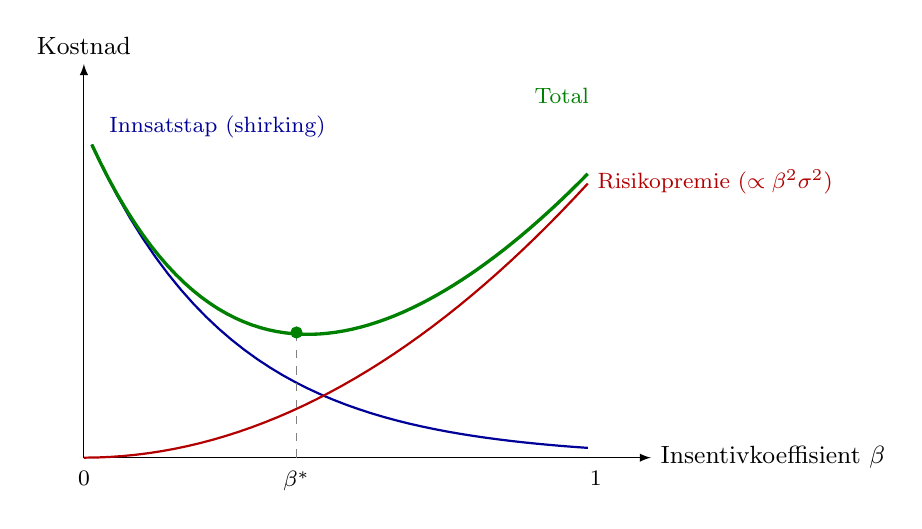
\begin{tikzpicture}[>=latex, every node/.style={font=\small}]
  % Akser
  \draw[->] (0,0) -- (7.2,0) node[right] {Insentivkoeffisient $\beta$};
  \draw[->] (0,0) -- (0,5.0) node[above] {Kostnad};
  % Markering 0 og 1 på x-aksen
  \node[below, font=\footnotesize] at (0,-0.05) {$0$};
  \node[below, font=\footnotesize] at (6.5,-0.05) {$1$};
  % Innsats-tap (synker når β øker)
  \draw[thick, blue!60!black, domain=0.1:6.4, samples=40]
    plot (\x, {4.2*exp(-0.55*\x)});
  \node[blue!60!black, font=\footnotesize, right] at (0.2,4.2) {Innsatstap (shirking)};
  % Risikopremie (stiger med β²)
  \draw[thick, red!70!black, domain=0:6.4, samples=40]
    plot (\x, {0.085*\x*\x});
  \node[red!70!black, font=\footnotesize, right] at (6.4,3.5) {Risikopremie ($\propto \beta^2 \sigma^2$)};
  % Total kostnad (sum) -- U-formet
  \draw[very thick, green!50!black, domain=0.1:6.4, samples=60]
    plot (\x, {4.2*exp(-0.55*\x) + 0.085*\x*\x});
  \node[green!50!black, font=\footnotesize, right] at (5.6,4.6) {Total};
  % β*-markering
  \draw[dashed, gray] (2.7,0) -- (2.7,1.59);
  \filldraw[green!50!black] (2.7,1.59) circle (2pt);
  \node[below, font=\bfseries\footnotesize] at (2.7,-0.05) {$\beta^*$};
\end{tikzpicture}
\caption{\textbf{Trade-offen risikodeling vs.\ insentiver.} Ved $\beta = 0$ (fastlønn): effektiv risikodeling, men maksimal shirking. Ved $\beta = 1$ (full residual claimancy): null shirking, men risikopremien koster prinsipalen $r\sigma^2/2$. Second-best $\beta^*$ minimerer summen og ligger strengt mellom 0 og 1. [SLIDE -- BSZ kap.\ 15, slide 7]}
\end{figure}

\subsection*{Eksempler}
\begin{itemize}\setlength{\itemsep}{2pt}
\item \textbf{Aksjonær vs.\ CEO i Norsk Hydro:} Aksjonær har portefølje med mange selskaper -- LME-aluminiumspris-risiko vaskes delvis ut. CEO har $\sim 80$\% av sin formue/humankapital bundet i Hydro $\Rightarrow$ risikoavers $\Rightarrow$ stor andel fast lønn + relative måltall mot peer-gruppe. [EKS]
\item \textbf{Sykehjemslege:} Output (pasientutfall) avhenger sterkt av eksogen helse hos pasienten ($\sigma^{2}$ stor). Risikodeling tilsier nesten ren fastlønn -- som er løsningen norsk offentlig sektor faktisk velger. [EKS]
\item \textbf{Hedgefond-trader (2$+$20-struktur):} Lite risikoavers, høy alfa, men $\sigma^{2}$ stor. Løsningen: ``high water mark'' og deferred compensation -- filtrerer ut deler av risiko og forhindrer asymmetrisk opp-/nedside (ekvivalent til indeksert opsjon). [EKS]
\end{itemize}

\subsection*{Kobling til søyle og andre teorier}
Søyle: \SThree\ (kontraktsdesignet legger fast risikofordelingen) med innslag av \STwo\ (måltallets støy bestemmer $\sigma^{2}$). Relaterte: \thref{optimal-effort-model}{Optimal effort-modell}, \thref{principal-agent}{Principal-agent}, \thref{incentive-coefficient}{Incentive coefficient}, \thref{fixed-vs-variable-pay}{Fast vs.\ variabel lønn}, \thref{informativeness-principle}{Informativeness-prinsippet}, \thref{moral-hazard}{Moral hazard}, \thref{agency-costs}{Agency costs}, \thref{costless-contracting}{Costless contracting} (first-best-referansen), \thref{costly-contracting}{Costly contracting}.

\paragraph{Brukt i spørsmål:} Q09, Q14, Q15.

% !TEX root = ../main.tex
\section{Præstationsuafhængig vs.\ variabel lønn ($W_0$ vs.\ $\beta Q$)}\label{thr:fixed-vs-variable-pay}

\paragraph{Definisjon.} Lønnskontrakten $W=W_0+\beta Q$ består av to konseptuelt forskjellige komponenter: $W_0$ er den \emph{præstationsuafhængige} (faste) lønnen, uavhengig av prestasjonen, mens $\beta Q$ er den \emph{variable} delen, hvor $\beta\in[0,1]$ er incitamentskoefficienten og $Q$ prestasjonsmålet. De to delene tjener \emph{ulike} formål i kontraktsdesignet og må analyseres separat. [SLIDE]

\subsection*{Forklaring}

I optimal effort-modellen (\thref{optimal-effort-model}{se modell A}) er agentens FOC:
\[
\beta\alpha\;=\;c'(e^{*}).
\]
$W_0$ faller ut. Det er en \emph{ren nivåvariabel}: den endrer agentens forventede inntekt uten å vri marginalbeslutningen om innsats. $\beta Q$ er derimot \emph{ren marginalvariabel}: den vrir innsats fordi marginal lønn øker med $\beta\alpha$ per enhet innsats. [SLIDE]

\textbf{Rollen til $W_0$ -- tre funksjoner.}
\begin{enumerate}\setlength{\itemsep}{1pt}
\item \textbf{Participation / IR-skranke.} $W_0$ justeres slik at agentens sikkerhetsekvivalent når reservasjonsnytten $\overline{U}$. Hvis $W_0$ er for lav, takker agenten nei.
\item \textbf{Risikopremie-kompensasjon.} Når agenten bærer risiko ($\beta>0$), pålegger hun seg en risikopremie $\tfrac{r}{2}\beta^{2}\sigma^{2}$. $W_0$ må heves for å kompensere for dette, ellers brytes IR-skranken.
\item \textbf{Forsikring / risikodeling.} Høy $W_0$ overfører eksogen risiko fra agenten til prinsipalen -- effektiv risikodeling, særlig når prinsipalen er diversifisert.
\end{enumerate}
$W_0$ vrir altså \emph{ikke} innsats, men er likevel nødvendig for at kontrakten skal fungere. [BOK]

\textbf{Rollen til $\beta Q$ -- to funksjoner.}
\begin{enumerate}\setlength{\itemsep}{1pt}
\item \textbf{Innsats-vridning (incentive).} Vrir agentens valg via $e^{*}=e^{*}(\beta)$.
\item \textbf{Risikoeksponering.} Bringer eksogen $\mu$-risiko inn i agentens lønn. Dette er kostnaden ved å bruke insentivlønn.
\end{enumerate}
Det er nettopp denne todelte funksjonen som skaper insentiv-risiko-trade-offen i \thref{risk-sharing}{risikodeling}. [SLIDE]

\textbf{Hvorfor begge komponenter trengs.}
\begin{itemize}\setlength{\itemsep}{1pt}
\item \textbf{Bare $W_0$ (ren fastlønn):} Ingen marginalt insentiv $\Rightarrow$ agenten velger minimal innsats (shirking). Effektiv risikodeling, men null produksjonsgevinst. \thref{moral-hazard}{Moral hazard} ikke håndtert.
\item \textbf{Bare $\beta Q$ (ren prestasjonslønn, $W_0=0$ eller negativ ``franchise fee''):} Agenten må kjøpe seg inn. Maksimal innsats hvis $\beta=1$, men hele $\mu$-risikoen lastes på agenten, som krever stor risikopremie. Realistisk kun for risikonøytrale agenter eller helt observerbart $e$.
\item \textbf{Hybrid (normen):} $W_0$ dekker IR + risikopremie; $\beta Q$ vrir innsats. Second-best-løsning.
\end{itemize}

\subsection*{Kjerneforutsetninger}
\begin{itemize}\setlength{\itemsep}{1pt}
\item Lineær kontrakt og lineær teknologi.
\item Reservasjonsnytte $\overline{U}$ er positiv (ellers $W_0$ kan settes til null).
\item $W_0$ er tidsmessig stabil -- ikke renforhandlet hver gang $\beta$ endres (ratchet effect ignorert).
\item Agenten kan ikke ``flyttes'' kostnadsfritt mellom kontrakter (ellers konkurrerer arbeidsmarkedet bort $W_0$).
\end{itemize}

\subsection*{Muligheter}
\begin{itemize}\setlength{\itemsep}{1pt}
\item Gir et klart språk for å diskutere lønnsdesign: $W_0$ for deltakelse og risiko; $\beta$ for innsats.
\item Forklarer hvorfor fastlønn og variabel lønn ikke er substitutter -- de gjør forskjellige ting.
\item Lar oss analysere effekter av endringer separat (f.eks.\ regulering av variabel lønn i banksektoren -- EU bonus-cap -- påvirker $\beta$ men må kompenseres med høyere $W_0$, som forklarer empirisk drift mot ``role-based pay'').
\item Forklarer hvorfor \emph{lønnsforhøyelse} (i $W_0$) ikke nødvendigvis gir mer innsats -- en klassisk leder-villfarelse.
\end{itemize}

\subsection*{Begrensninger og kritikk}
\begin{itemize}\setlength{\itemsep}{1pt}
\item Skarpt skille mellom $W_0$ og $\beta Q$ forutsetter linearitet -- terskler, stair-step-bonus og opsjoner gjør at fastlønnen \emph{kan} indirekte påvirke insentiver (når den nærmer seg gulvet i en bonusplan).
\item Atferdsforskning: høy $W_0$ kan ha \emph{gave-utveksling}-effekt (Akerlof) -- ansatte yter mer enn FOC tilsier av lojalitet/normer. Modellen fanger ikke dette.
\item Karriere-insentiver, status og ``promotion tournament'' fungerer som implisitte variable komponenter selv når formelt $\beta=0$ -- den lineære modellen underestimerer faktiske insentiver i tariffjobber.
\item Skattelovgivning og pensjonsordninger gjør faktisk verdi av $W_0$ vs.\ $\beta Q$ asymmetrisk -- modellen ignorerer dette.
\item Internasjonale forskjeller (USA: mer $\beta Q$; Skandinavia/Tyskland: mer $W_0$) viser at institusjonelle og normative faktorer dominerer FOC i mange tilfeller.
\end{itemize}

\subsection*{Modell / illustrasjon}

\begin{center}
\renewcommand{\arraystretch}{1.15}
\begin{tabular}{@{}p{3.0cm}p{4.2cm}p{6.5cm}@{}}
\toprule
\textbf{Komponent} & \textbf{Hva den gjør} & \textbf{Hva den \emph{ikke} gjør} \\
\midrule
$W_0$ (fast) & Oppfyller IR, kompenserer risikopremie, gir forsikring & Vrir ikke marginal innsats \\
$\beta Q$ (variabel) & Vrir innsats, kobler agent til prinsipalens mål & Gir ikke effektiv risikodeling alene \\
\bottomrule
\end{tabular}
\end{center}

\begin{figure}[h]
\centering

\includegraphics[width=0.55\linewidth]{BSZ_kap_15_2026/by_slide/slide_020/BSZ_kap_15_2026_slide_020_asset_01_image7.jpeg}
\caption{Lønnskontrakten dekomponert: fast del ($W_0$) + variabel del ($\beta Q$). [SLIDE -- BSZ kap.\ 15, slide 20]}
\end{figure}

\subsection*{Eksempler}
\begin{itemize}\setlength{\itemsep}{2pt}
\item \textbf{Norsk tariffstilling (sykepleier):} Alt $W_0$, $\beta\approx 0$. Output (omsorgskvalitet) er umålbart, agenten er risikoavers, og fagforening favoriserer kollektive ordninger. [EKS]
\item \textbf{Norsk Hydro-bonusplan for divisjonsledelse:} Grunnlønn (~70\%) + årsbonus knyttet til divisjons-EBITDA (~20\%) + LTI (~10\%). Hybrid -- $W_0$ dekker risikopremien, $\beta Q$ vrir innsats. [EKS]
\item \textbf{Ren provisjonsselger (uten grunnlønn):} $W_0=0$, $\beta=1$ på salgsverdi. Krever lav risikoaversjon og høy målbarhet -- bare anvendelig i bransjer som dør-til-dør-salg eller renessanseaktige modeller. [EKS]
\item \textbf{Bankenes EU bonus-cap (2014):} Variabel del begrenset til $100$--$200$\% av $W_0$. Banker responderte med å heve $W_0$ (``allowances'') for å beholde total lønn -- modellen forutsa nettopp dette: $W_0$ og $\beta Q$ er ikke perfekte substitutter, men kan tilpasses så total CE forblir. [EKS]
\end{itemize}

\subsection*{Kobling til søyle og andre teorier}
Søyle: \SThree\ (kontraktens designvariabler). Relaterte: \thref{optimal-effort-model}{Optimal effort-modell}, \thref{incentive-coefficient}{Incentive coefficient}, \thref{risk-sharing}{Risk sharing}, \thref{principal-agent}{Principal-agent}, \thref{moral-hazard}{Moral hazard}, \thref{agency-costs}{Agency costs}, \thref{informativeness-principle}{Informativeness-prinsippet}.

\paragraph{Brukt i spørsmål:} Q09, Q14.

% Q10 theories
% !TEX root = ../main.tex
\section{Formålene med individuell prestasjonsmåling og -belønning}\label{thr:performance-measurement-purposes}

\paragraph{Definisjon.} Individuell prestasjonsmåling og -belønning er den systematiske kartleggingen og evalueringen av en ansatts innsats og resultater, koblet til en kompensasjons- eller anerkjennelsesmekanisme. BSZ kap.\ 16 angir fire \emph{simultane} formål med slik måling: (i) gi medarbeideren \emph{feedback}, (ii) støtte \emph{koordinasjon} på tvers av enheter, (iii) gi grunnlag for \emph{belønning og sanksjon}, og (iv) støtte den øvrige \thref{organizational-architecture}{organizational architecture} ved å binde S1, S2 og S3 sammen. [SLIDE]

\subsection*{Forklaring}

Prestasjonsmåling er aldri kun et regnskapsmessig spørsmål -- det er en av de tre søylene som hele organisasjonsdesignet hviler på. BSZ insisterer på at \emph{samme} måltall ofte må tjene flere formål samtidig, og at det er denne flerbruken som gjør design vanskelig: et mål som er fint til feedback (rik, kvalitativ, kontinuerlig) kan være ubrukelig som bonusgrunnlag (krever verifiserbarhet, juridisk holdbarhet), og omvendt. Læreboken understreker at prestasjonsmålet må passe med (a) \emph{kompensasjonsstrukturen} -- ellers blir insentivkoeffisienten (\thref{incentive-coefficient}{$\beta$ i $W = W_0 + \beta Q$}) feilkalibrert -- og (b) \emph{beslutningsrettighetene} -- ellers brytes \thref{controllability-principle}{controllability-prinsippet} og lederen demotiveres. [SLIDE/BOK]

De fire formålene er:
\begin{enumerate}\setlength{\itemsep}{3pt}
\item \textbf{Feedback (læring).} Den ansatte trenger informasjon om hvor hun står for å justere atferd. Dette formålet handler om \emph{ex post} forståelse -- 360-graders evaluering, utviklingssamtaler, kontinuerlig coaching. Belønning er ikke nødvendig; det viktige er at signalet er rikt og rettidig.
\item \textbf{Koordinasjon.} Felles måltall fungerer som retningsangiver: når salg og produksjon måles på samme leveringsindikator, koordinerer de uten direkte forhandling. Måling er her et språk for hva organisasjonen prioriterer.
\item \textbf{Belønning og sanksjon.} Måltallet er input til kompensasjon, forfremmelse, fyring. Dette formålet stiller harde krav: målet må være verifiserbart, kontrollerbart og informativt om innsats (jf.\ \thref{informativeness-principle}{informativeness-principle}). Det er her gaming-faren er størst.
\item \textbf{Støtte til organisatorisk arkitektur.} Måltallet binder beslutningsrett (S1) og insentiv (S3) sammen. Endrer man et ben i skammelen, må måltallet justeres -- ellers oppstår misalignment og residual loss eksploderer (jf.\ \thref{agency-costs}{agency costs}).
\end{enumerate}
[SLIDE]

\subsection*{Kjerneforutsetninger}
\begin{itemize}
\item Innsats $e$ er ikke direkte observerbar -- man må måle et utfall $Q = \alpha e + \mu$ som proxy (jf.\ \thref{principal-agent}{principal-agent-modellen}).
\item Det finnes et meningsfullt skille mellom innsatsdrevne og eksogene komponenter av utfallet (\thref{controllability-principle}{controllability}).
\item Måling er kostbar -- det er en marginal benefit / marginal cost-avveining hvor presist man kan måle.
\item Den ansatte er minst delvis rasjonell og responderer på målene som settes (``you get what you measure'').
\item Måltallet kan brukes til mer enn ett formål samtidig, men noen ganger må man velge.
\end{itemize}
[SLIDE/BOK]

\subsection*{Muligheter}
\begin{itemize}
\item Forklarer hvorfor selskaper ofte har \emph{separate} systemer for utviklingsfeedback og bonus -- de fire formålene drar i ulike retninger.
\item Begrunner balansert målekort (Kaplan \& Norton): finansielle mål alene treffer kun belønningsformålet, ikke koordinasjon eller læring.
\item Begrunner bonusbanker, deferred compensation og claw-backs -- de redder belønningsformålet uten å ødelegge koordinasjons- og læringsformålet.
\item Forklarer hvorfor 360-evalueringer ofte holdes adskilt fra lønnsoppgjør: rene feedback-data blir forurenset hvis de også er bonusgrunnlag.
\item Gir et diagnostisk rammeverk: ``Hvilket formål svikter i vårt målesystem?'' kan stilles direkte.
\end{itemize}

\subsection*{Begrensninger og kritikk}
\begin{itemize}
\item \textbf{Trade-off mellom formålene er reell, ikke teoretisk.} Et måltall optimert for belønning (verifiserbart, kvantitativt, individuelt) er ofte dårlig til koordinasjon (krever team og delte mål) og læring (krever rikt kvalitativt innhold).
\item \textbf{Måleparadokset (Goodhart's law).} ``Når en måling blir et mål, slutter den å være et godt mål.'' Et godt feedback-mål blir et dårlig belønningsmål så snart bonus knyttes til det.
\item \textbf{Multitasking-problem (Holmström \& Milgrom 1991).} Hvis bare ett av flere jobbaspekter måles, vrir agenten innsats mot det målbare. Eksempel: lærer måles på elevenes prøveresultat $\Rightarrow$ ignorerer kreativitet og samarbeid.
\item \textbf{Ratchet og gaming} er endogene konsekvenser av at samme mål brukes til alle fire formål (jf.\ \thref{ratchet-effect}{ratchet-effect} og \thref{gaming-in-performance-measurement}{gaming}).
\item \textbf{Subjektive evalueringer kan virke uretferdige} -- gir påvirkningskostnader og supervisor shirking (jf.\ \thref{subjective-vs-objective-performance}{subjektiv vs.\ objektiv}).
\item \textbf{Risikoallokering.} Sterk bobus-knytting overfører støy ($\mu$) til en risikoavers agent, som krever risikopremie. Læring og koordinasjon krever ikke slik risikoeksponering.
\end{itemize}

\subsection*{Modell / illustrasjon}

\begin{figure}[h]
  \centering
  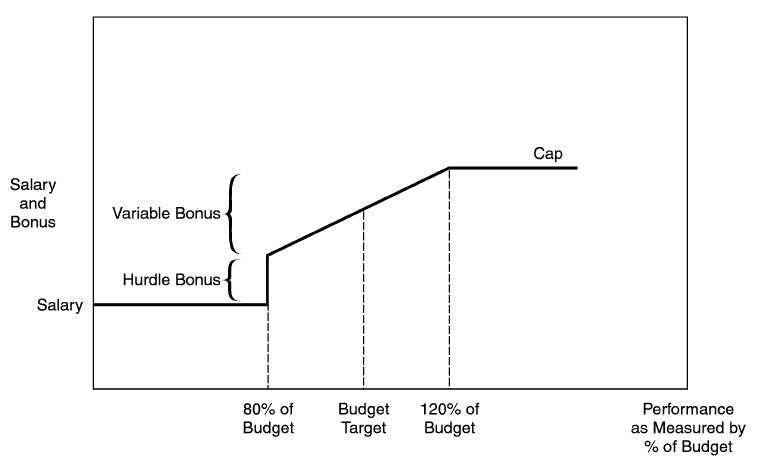
\includegraphics[width=0.55\linewidth]{BSZ_kap_16/by_slide/slide_014/BSZ_kap_16_slide_014_asset_01_image2.png}
  \caption{Typisk bonusplan: fast lønn + hurdle bonus + variabel bonus + cap. Illustrerer hvordan prestasjonsmåling kobles til belønning. (BSZ kap.\ 16, slide 14) [SLIDE]}
\end{figure}

I lærebokens grunnmodell er ansattes ytelse $Q = \alpha e + \mu$ der $\alpha$ er produktivitet, $e$ innsats og $\mu$ støy. Kompensasjonen $W = W_0 + \beta Q$ knytter belønning til ytelse via insentivkoeffisient $\beta \in [0, 1]$. De fire formålene henter ulike egenskaper fra denne formelen:

\begin{center}
\renewcommand{\arraystretch}{1.2}
\begin{tabular}{@{}p{3.4cm}p{4.5cm}p{6.0cm}@{}}
\toprule
\textbf{Formål} & \textbf{Hovedvariabel} & \textbf{Designkrav til $Q$} \\
\midrule
Feedback & Informasjonsinnhold i $Q$ & Rikt, kontinuerlig, kvalitativt; støy tolerert. \\
Koordinasjon & Felles og kommunisert $Q$ & Synlig, retningsgivende, like for tilstøtende enheter. \\
Belønning/sanksjon & $\beta$ og verifiserbarhet av $Q$ & Kontrollerbart, juridisk holdbart, lite støy. \\
Arkitekturstøtte & Kobling $Q \to W$ til S1 og S3 & Måltall som speiler delegerte beslutningsrettigheter. \\
\bottomrule
\end{tabular}
\end{center}
[SLIDE]

\subsection*{Eksempler}
\begin{itemize}
\item \textbf{Equinor (NO).} Bruker tre adskilte systemer: kontinuerlig coaching (feedback), People@Equinor måltall for HMS og leveringspresisjon (koordinasjon på tvers av prosjektenheter), og STI/LTI bonusprogram knyttet til konsernresultat (belønning). Dette er en lærebokmessig oppdeling: ulike mål for ulike formål. [EKS]
\item \textbf{Microsoft (etter 2013).} Avskaffet ``stack ranking''-bonussystemet som kollapset alle fire formål inn i én årlig rangering. Erstattet det med separat ``Connect''-system (feedback) og en mer kvalitativ kompensasjonsdiskusjon. Eksempel på at \emph{adskillelse} av formålene øker både motivasjon og koordinasjon. [EKS]
\item \textbf{MBO (Management by Objectives, Drucker).} Klassisk eksempel på at \emph{koordinasjons-} og \emph{belønningsformål} slås sammen: målene settes i dialog (koordinasjon) og kobles til bonus (belønning) -- men dette skaper også ratchet-faren. [BOK]
\item \textbf{Sykehus-DRG-system.} Aktivitetsbasert finansiering måler antall behandlinger -- godt til koordinasjon og kontroll, men dårlig til feedback om kvalitet. Klassisk multitasking-problem. [EKS]
\end{itemize}

\subsection*{Kobling til søyle og andre teorier}
Søyle: \STwo\ primært, men hele poenget er at S2 ikke kan designes alene -- må kobles til \SOne\ (kontrollerbarhet, beslutningsrett) og \SThree\ (kompensasjonskobling). Relaterte teorier: \thref{principal-agent}{Principal-Agent}, \thref{moral-hazard}{Moral hazard}, \thref{controllability-principle}{Controllability-prinsippet}, \thref{informativeness-principle}{Informativeness-prinsippet}, \thref{ratchet-effect}{Ratchet-effekten}, \thref{gaming-in-performance-measurement}{Gaming}, \thref{absolute-vs-relative-performance}{Absolutt vs.\ relativ prestasjonsmåling}, \thref{subjective-vs-objective-performance}{Subjektiv vs.\ objektiv prestasjonsmåling}, \thref{agency-costs}{Agency costs}, \thref{responsibility-centers}{Responsibility centers}, \thref{organizational-architecture}{Organizational architecture}.

\paragraph{Brukt i spørsmål:} Q10.

% !TEX root = ../main.tex
\section{Ratchet-system og ratchet-effekten}\label{thr:ratchet-effect}

\paragraph{Definisjon.} Et \emph{ratchet-system} er en målsettingsmekanisme der fremtidige prestasjonsmål bygges direkte på inneværende periodes faktiske ytelse -- jo bedre du presterer i år, jo strammere mål får du neste år. \emph{Ratchet-effekten} er agentens rasjonelle respons: hun holder igjen innsatsen i dag for å unngå at standarden skrus opp i morgen. Den ekstreme formen heter \emph{sandbagging} -- bevisst underprestering for å skape lettere fremtidige mål. [SLIDE]

\subsection*{Forklaring}

Ratchet-effekten er et dynamisk insentivproblem: en ettperiodisk \thref{principal-agent}{principal-agent}-kontrakt bryter sammen når både prinsipal og agent vet at \emph{neste} periodes kontrakt skrives på grunnlag av \emph{denne} periodens utfall. Selv en agent med høyt innsatsnivå har incentiv til å skjule kapasiteten sin, fordi å avsløre den koster henne i alle fremtidige perioder. Mekanismen er analog til en skrallsnøkkel (en \emph{ratchet}): bevegelsen går bare én vei -- målet skrus opp, aldri ned -- og fastlåses der. [SLIDE/BOK]

Begrepet ble først dokumentert systematisk i analyser av sovjetisk planøkonomi (Berliner 1957, Weitzman 1980): fabrikksjefer som leverte over plan i år fikk strammere plan neste år. Resultatet var en kultur for konstant ``95\,\% leveranse'' -- aldri 100 \% -- selv om reell kapasitet var langt høyere. Det samme mønsteret ses i moderne salgsbudsjetter, regnskapsmessige budsjetter med årlig påslag, og i offentlig sektor med årlige effektivitetskrav (``Rattle the Cage''-effekten, ABE-kravet i NO). [BOK]

Ratchet-effekten er en spesifik form for \thref{gaming-in-performance-measurement}{gaming}: i stedet for å manipulere selve målingen, manipulerer agenten \emph{tempoet} hvori god prestasjon avsløres. Den er også en direkte konsekvens av at samme målesystem brukes til både feedback og belønning -- jf.\ \thref{performance-measurement-purposes}{formålene med prestasjonsmåling}. [SLIDE]

\subsection*{Kjerneforutsetninger}
\begin{itemize}
\item \textbf{Gjentakelse:} Spillet mellom prinsipal og agent gjentas; én-periodisk kontrakt ville ikke gi ratchet.
\item \textbf{Asymmetrisk informasjon:} Prinsipalen kjenner ikke agentens sanne kapasitet og må lære den av observerte resultater (\emph{ratcheting from history}).
\item \textbf{Mangel på commitment:} Prinsipalen kan ikke troverdig binde seg til \emph{ikke} å bruke årets resultat når neste års mål settes -- selv om det ville være optimalt ex ante.
\item \textbf{Rasjonell, fremtidsorientert agent:} Agenten verdsetter fremtidige perioders nytte tilstrekkelig høyt til at sandbagging lønner seg.
\item \textbf{Liten konkurransepress:} Ratchet-effekten er sterkest når agenten ikke kan erstattes -- ellers vinner en konkurrent ved å vise sin sanne kapasitet.
\end{itemize}

\subsection*{Muligheter (hva forklarer teorien?)}
\begin{itemize}
\item Forklarer hvorfor mange budsjetter ``alltid'' treffer 95--100 \% av målet -- distribusjonen er truncated nedenfra og over.
\item Forklarer hvorfor selskaper introduserer flerårige incentivprogram (LTI), bonusbanker eller fastsatte måltallsformler.
\item Forklarer hvorfor relative og eksterne benchmarks (\thref{absolute-vs-relative-performance}{relative performance evaluation}) er attraktive -- de bryter koblingen mellom \emph{egen} prestasjon og \emph{eget} fremtidig mål.
\item Forklarer hvorfor private equity-eide selskaper ofte gir kraftig produktivitetshopp etter overtakelse: nye eiere bryter den implisitte ratchet-kontrakten.
\item Jensen-kritikken av budgetbaserte bonuser (BSZ kap.\ 16) hviler direkte på ratchet-logikken: når neste års budsjett settes fra årets resultat, blir budsjettet både plan- og belønningsverktøy, og begge formål korrumperes.
\end{itemize}

\subsection*{Begrensninger og kritikk}
\begin{itemize}
\item \textbf{Empirisk størrelse er omstridt.} Sandbagging er vanskelig å skille fra reell kapasitetsbegrensning -- studier overestimerer ofte ratchet-effektens omfang.
\item \textbf{Karrierebekymringer kan oppveie ratchet.} Yngre ansatte ønsker å vise topp-prestasjon for å bli forfremmet, selv om det øker fremtidig målnivå. \emph{Career concerns} (Holmström 1982) trekker motsatt vei.
\item \textbf{Implicit relational contracts.} Hvis prinsipal og agent har et langvarig tillitsforhold, kan ratchet-fellen unngås ved norm: ``Vi straffer deg ikke for å overlevere.'' Vanskelig å håndheve, men empirisk observert.
\item \textbf{Løsningen kan skape nye problemer.} Eksterne benchmarks introduserer relativ måling med egne problemer (sabotasje, manipulasjon av peer-gruppe).
\item \textbf{Ratchet kan også være effektivt.} Hvis kapasiteten faktisk endrer seg over tid, er det rasjonelt å oppdatere mål -- skillet mellom ``rettferdig oppdatering'' og ``ratchet-utnyttelse'' er ikke skarpt.
\item \textbf{Modellene er ofte stiliserte.} Reelle bonusbudsjetter har glattere mekanismer (kapp, bunner, sjettesninger) som demper, men ikke fjerner, ratchet-effekten.
\end{itemize}

\subsection*{Modell / illustrasjon}

I et stilisert toperiode-spill: agenten velger $e_1$ i periode 1 vel vitende om at neste periodes mål blir $\bar{Q}_2 = \gamma Q_1$ for $\gamma \in (0, 1]$. Optimal innsats er derfor lavere enn ved engangsspill -- agenten internaliserer at $\partial \bar{Q}_2 / \partial Q_1 > 0$ koster henne nytte i periode 2. Jensen foreslår at man bryter koblingen ved å gjøre bonus \emph{lineær} og uavhengig av fastsatt budsjett:

\begin{figure}[H]
  \centering
  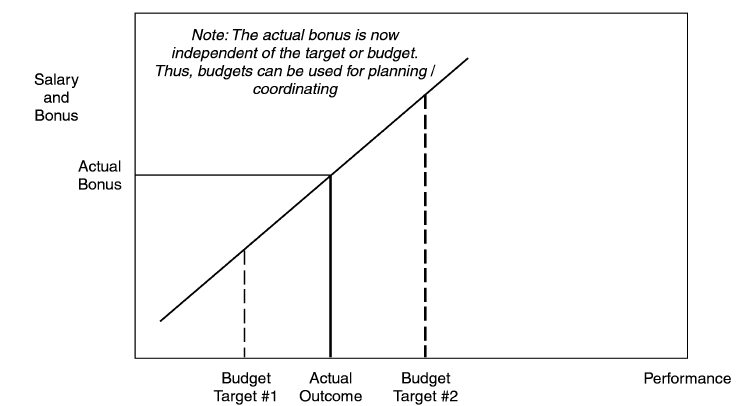
\includegraphics[width=0.65\linewidth]{BSZ_kap_16/by_slide/slide_016/BSZ_kap_16_slide_016_asset_01_image3.png}
  \caption{Jensens forslag: lineær pay-for-performance der bonus er uavhengig av målet. Når bonuskurven ikke skifter med budsjettet, forsvinner motivasjonen for sandbagging og ratchet-tilpasning. (BSZ kap.\ 16, slide 16) [SLIDE]}
\end{figure}

\subsection*{Eksempler}
\begin{itemize}
\item \textbf{Sovjetisk fabrikkproduksjon (Berliner, Weitzman).} Direktører leverte konsekvent litt over plan, aldri mye over, for å unngå strammere plan neste år. Klassisk historisk dokumentasjon. [BOK]
\item \textbf{IBM-salgskvoter (1990-tallet).} Salgsledere som overperformerte fikk høyere kvoter neste år; resultatet var en bransjenorm om ``akkurat over kvote''. Endret med innføring av flerårige LTI-program. [EKS]
\item \textbf{Norske kommunale ABE-krav (effektiviseringskrav).} Etaten som leverer effektiviseringsgevinst får krav om mer neste år. Etater holder igjen tiltak til ``nødvendige år''. [EKS]
\item \textbf{Mærsk CAPEX-budsjettering.} Hvis PtX-divisjonen oppnår alle prosjektmilestones år 1, kan konsernet skru opp neste års mål. Risiko for sandbagging ved tidsangivelse. [CASE]
\item \textbf{Vy/NSB og punktlighet.} Hvis 95 \% punktlighet utløser bonus og neste års mål, har ledelsen incentiv til å ikke avsløre at 98 \% er mulig. [EKS]
\end{itemize}

\subsection*{Kobling til søyle og andre teorier}
Søyle: \STwo\ (måltallsdesign) og \SThree\ (bonusstrukturer). Relaterte teorier: \thref{performance-measurement-purposes}{Formålene med prestasjonsmåling} (ratchet er konsekvens av flerbruk), \thref{gaming-in-performance-measurement}{Gaming} (samme familie), \thref{absolute-vs-relative-performance}{Absolutt vs.\ relativ prestasjonsmåling} (relativ måling er ratchet-løsning), \thref{principal-agent}{Principal-Agent}, \thref{moral-hazard}{Moral hazard}, \thref{controllability-principle}{Controllability-prinsippet}, \thref{responsibility-centers}{Responsibility centers}, \thref{incentive-coefficient}{Insentivkoeffisient}.

\paragraph{Brukt i spørsmål:} Q10.

% !TEX root = ../main.tex
\section{Gaming og horisontproblem}\label{thr:gaming-in-performance-measurement}

\paragraph{Definisjon.} \emph{Gaming} er den atferden der en ansatt manipulerer prestasjonsmålet i stedet for å skape den underliggende verdien målet skal speile. \emph{Horisontproblemet} er en spesifikk form: kortsiktig optimering av et målt utfall som ofrer langsiktig verdi. Begge er opportunistisk respons på imperfekte målesystemer og er et empirisk uttrykk for Goodhart's law: ``Når et mål blir et bonusmål, slutter det å være et godt mål.'' [SLIDE]

\subsection*{Forklaring}

Gaming oppstår når tre forhold er oppfylt samtidig: (i) målet er imperfekt korrelert med den verdi prinsipalen egentlig vil oppnå, (ii) det er rom for å påvirke det målte uten å påvirke verdien, og (iii) bonus eller karriereutfall er sterkt koblet til målet. Klassiske former er regnskapsmanipulasjon (\emph{earnings management}), shifting av kostnader mellom perioder, hopping i prosjektklassifisering, og direkte juks. Horisontproblemet er en mildere variant: agenten foretar reelle, men kortsiktig orienterte handlinger -- f.eks.\ utsetter vedlikehold for å pynte på årets EBITDA -- som leverer på målet men reduserer total firmaverdi. [SLIDE/BOK]

BSZ kap.\ 16 fremhever at gaming er en endogen konsekvens av målesystemets design. Det er ikke et tegn på dårlig moral hos den ansatte; det er en \emph{forventet} respons på sterke insentiver og imperfekt måling. Derfor er løsningen ikke ``mer overvåkning'' alene, men \emph{strukturelt smartere måling}: balansert målekort, bonusbanker, flerårig perspektiv, subjektiv overstyringsmulighet, multitasking-bevisst design (Holmström \& Milgrom 1991: når flere oppgaver konkurrerer om innsats, må bonusrelativitet mellom dem balanseres -- ellers vrir agenten innsats mot det målbare). [SLIDE]

Den teoretiske roten ligger i den støyete prestasjonsmodellen $Q = \alpha e + \mu$. Når $Q$ kan manipuleres uten å øke $e$ -- altså når agenten har en ekstra ``manipulasjonshandling'' $m$ som flytter $Q$ uten å skape verdi -- vil enhver sterk bonus på $Q$ stimulere $m$ i tillegg til $e$. Resultatet er det BSZ kaller \emph{dysfunctional behavior}. [BOK]

\subsection*{Kjerneforutsetninger}
\begin{itemize}
\item Måltallet er en imperfekt proxy for sann verdiskaping (gap mellom $Q$ og det prinsipalen faktisk verdsetter).
\item Agenten kan påvirke målingen på måter som ikke er observerbare eller kostbart verifiserbare.
\item Sterk bonus eller karrierebelønning kobler agentens nytte direkte til $Q$.
\item Multitasking: agenten utfører flere oppgaver; bare noen måles.
\item Tidshorisonten i bonusen er kortere enn tidshorisonten for verdien (horisontproblem).
\end{itemize}

\subsection*{Muligheter (hva forklarer/løser teorien?)}
\begin{itemize}
\item Forklarer hvorfor regnskapsskandaler ofte oppstår i selskaper med aggressive bonusprogram knyttet til EPS-mål (Enron, WorldCom).
\item Forklarer hvorfor offentlige KPI-er gir uventede vridninger (NHS A\&E 4-timersmål, skolers ``teaching to the test'').
\item Begrunner bruk av \emph{balanced scorecard} (Kaplan \& Norton): finansielle + kunde + interne prosess + læringsmål reduserer manipulasjonsrom på hver enkelt akse.
\item Begrunner \emph{bonusbanker} og \emph{claw-back}: utsetter utbetaling så manipulasjon kan korrigeres senere.
\item Begrunner subjektiv ``overstyring'': når formelresultatet er åpenbart manipulert, kan en evaluator overstyre.
\item Forklarer hvorfor multitasking-jobber bør ha \emph{lavere} insentivvekt på det målbare (Holmström \& Milgrom): det reduserer skjevhet i innsatsallokeringen.
\end{itemize}

\subsection*{Begrensninger og kritikk}
\begin{itemize}
\item \textbf{Balansert målekort har egne problemer.} Mange mål kan gjøre prioritering uklar; agenten vrir mot det letteste, ikke det viktigste.
\item \textbf{Subjektiv overstyring} introduserer påvirkningskostnader og partiskhet (jf.\ \thref{subjective-vs-objective-performance}{subjektiv vs.\ objektiv}).
\item \textbf{Gaming er ikke alltid skadelig.} Noen ganger ``finner'' agenten en kreativ snarvei som faktisk skaper verdi -- skillet mellom innovasjon og gaming er ikke skarpt.
\item \textbf{Modellene antar opportunistisk agent.} Faktisk handler mange ansatte etter normer og identitet (\emph{intrinsic motivation}) som demper gaming uten formelle mekanismer.
\item \textbf{Løsningen kan bli verre enn problemet.} Detaljerte anti-gaming-regler øker compliance-kost, byråkrati og residual loss; balansen mot agency-costs (\thref{agency-costs}{agency costs}) er ikke triviell.
\item \textbf{Vanskelig å skille gaming fra dårlig flaks ex post.} En manager som leverer dårlig kvalitet kan hevde at det var marked, ikke vridd innsats.
\end{itemize}

\subsection*{Modell / illustrasjon}

Goodhart's law (1975) formaliseres av Holmström \& Milgrom (1991): for en agent med flere oppgaver $e_1, \dots, e_n$ der bare noen er målte, gjelder
\[ \beta_i^* \propto \frac{1}{1 + r \sigma_i^2} \cdot \frac{1}{1 + \text{spillover}_i} \]
-- jo flere ikke-målte oppgaver som påvirkes av $e_i$, desto \emph{lavere} bør insentivvekten på $e_i$ være. Sterk bonus på ett målbart mål gir gaming hvis andre verdiskapende aktiviteter blir fortrengt. [BOK]

Den klassiske horisontfellen ses i Jensens kritikk av budget-bonus-systemer:

\begin{figure}[h]
  \centering
  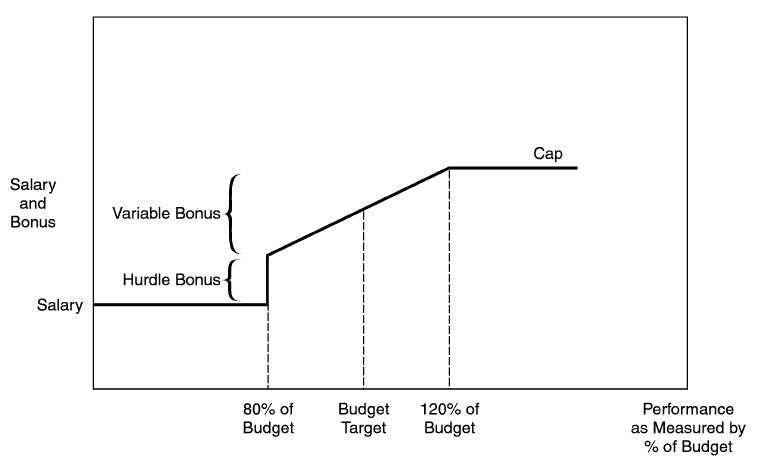
\includegraphics[width=0.65\linewidth]{BSZ_kap_16/by_slide/slide_014/BSZ_kap_16_slide_014_asset_01_image2.png}
  \caption{Tradisjonelt budget-bonus-system med ``hurdle'' ved 80\,\% og ``cap'' ved 120\,\%. Den knekkede formen skaper gaming: rett under hurdle har agenten incentiv til å skyve resultater til neste år; rett over cap har hun incentiv til å holde igjen. Jensens løsning er den lineære lønnen i illustrasjonen i \thref{ratchet-effect}{ratchet-effect}-filen. (BSZ kap.\ 16, slide 14) [SLIDE]}
\end{figure}

\subsection*{Eksempler}
\begin{itemize}
\item \textbf{Wells Fargo (US, 2016).} Aggressive cross-sell-kvoter for filialer utløste 3,5 mill.\ falske kundekontoer -- klassisk gaming. Bonus var sterkt knyttet til antall produkter pr.\ kunde; ansatte manipulerte målet uten å skape verdi. Endte med \$185 mill.\ bot og endring av kompensasjonsmodell. [EKS]
\item \textbf{Volkswagen Dieselgate (2015).} ``Defeat devices'' i motorstyringssystem -- gaming av utslippsmål uten å redusere faktisk utslipp. Eksempel på at gaming kan eskalere til regelrett juks. [EKS]
\item \textbf{NHS A\&E 4-timers ventetid (UK).} Sykehus klassifiserte pasienter som ``ferdig behandlet'' rett før 4-timersgrensen, deretter satte dem på ny venteliste. Klassisk re-klassifiserings-gaming. [EKS]
\item \textbf{Vy/NSB punktlighet (NO).} Tog hopper over små stasjoner for å nå punktlighetsmål på endestasjon -- horisontproblem og gaming kombinert. [EKS]
\item \textbf{Mærsk Power-to-X.} Hvis kortsiktig OPEX brukes som mål for prosjektledere, kan vedlikehold på elektrolysører utsettes for å pynte på årets tall -- klassisk horisontproblem. Løsning: milestone-basert måling og subjektiv kvalitetsratifisering. [CASE]
\item \textbf{Enron, WorldCom (US, 2001--2002).} Regnskapsmanipulasjon drevet av aksjebonus knyttet til kvartalsvis EPS -- ekstremvariant av horisontproblem. [EKS]
\end{itemize}

\subsection*{Kobling til søyle og andre teorier}
Søyle: \STwo\ (måletekniske valg) og \SThree\ (bonusdesign). Relaterte teorier: \thref{performance-measurement-purposes}{Formålene med prestasjonsmåling}, \thref{ratchet-effect}{Ratchet-effekten}, \thref{absolute-vs-relative-performance}{Absolutt vs.\ relativ prestasjonsmåling}, \thref{subjective-vs-objective-performance}{Subjektiv vs.\ objektiv prestasjonsmåling}, \thref{informativeness-principle}{Informativeness-prinsippet}, \thref{moral-hazard}{Moral hazard}, \thref{principal-agent}{Principal-Agent}, \thref{controllability-principle}{Controllability-prinsippet}, \thref{agency-costs}{Agency costs}, \thref{incentive-coefficient}{Insentivkoeffisient}.

\paragraph{Brukt i spørsmål:} Q10.

% !TEX root = ../main.tex
\section{Absolutt vs.\ relativ prestasjonsmåling}\label{thr:absolute-vs-relative-performance}

\paragraph{Definisjon.} \emph{Absolutt} prestasjonsmåling vurderer en ansatt (eller enhet) uavhengig av andre -- mot et forhåndsdefinert nivå, budsjett eller standard. \emph{Relativ} prestasjonsmåling vurderer den ansatte i forhold til en peer-gruppe: andre ansatte, andre divisjoner, eller eksterne benchmarks. Skillet handler om hva slags støy som filtreres ut av målet. [SLIDE]

\subsection*{Forklaring}

Den teoretiske begrunnelsen for relativ måling kommer fra Holmström (1979) \emph{informativeness principle}: bruk \emph{all} lavkost-informasjon som er korrelert med agentens innsats. Hvis to selgere i samme bransje begge rammes av en pandemi som halverer markedet, sier deres absolutte salgstall lite om innsats -- men forskjellen mellom dem sier mye. Relativ måling filtrerer altså bort felles sjokk ($\mu_{\text{common}}$) og gjør prestasjonsmålet mer informativt om innsats $e$. Konsekvensen i \thref{principal-agent}{principal-agent}-modellen er at man kan sette en høyere insentivkoeffisient \thref{incentive-coefficient}{$\beta$} uten å overlaste agenten med risiko -- billigere insentivkontrakt. [SLIDE/BOK]

Absolutt måling, derimot, har sin styrke der koordinasjon og samarbeid er viktigst. Når alle blir bedømt mot en felles standard og ikke mot hverandre, fjernes incentivet til å sabotere kolleger eller hamstre informasjon. Det er også enklere å kommunisere: ``Du skal selge for 10 millioner'' er lettere enn ``Du skal være blant topp 20 \% av selgerne''. [SLIDE]

I praksis brukes ofte en \emph{hybrid}: en absolutt komponent (treffer budsjett) kombinert med en relativ (rTSR -- relativ Total Shareholder Return -- mot peer-indeks). De fleste børsnoterte selskapers LTI-program er av denne typen. [BOK]

\subsection*{Kjerneforutsetninger}
\begin{itemize}
\item For relativ måling: peer-gruppen må være tilstrekkelig stor, sammenlignbar, og utsatt for samme felles sjokk som agenten.
\item For relativ måling: agentene må ikke kunne påvirke hverandres prestasjoner sterkt (lite kooperativ interaksjon), ellers vrir relativ måling mot sabotasje.
\item For absolutt måling: det må finnes en stabil, kalibrerbar standard. Når omgivelsene endrer seg sterkt, blir absolutt mål raskt utdatert (ratchet-fare).
\item Informativeness-prinsippet forutsetter at peer-prestasjon er korrelert med agentens støy, ikke med hennes innsats.
\item Risikoaversjon hos agenten -- ellers spiller risikodelingsargumentet for relativ måling mindre rolle.
\end{itemize}

\subsection*{Muligheter}
\begin{itemize}
\item \textbf{Relativ:} Filtrerer ut bransje-, marked- og makrosjokk. Reduserer risikopremie. Tournament-effekt motiverer topptalenter (Lazear \& Rosen 1981).
\item \textbf{Relativ:} Gir kontinuerlig benchmarking -- ingen ratchet-fare fra eget historie, siden målet flyttes av andres prestasjoner, ikke av egne.
\item \textbf{Absolutt:} Enkelt å forstå og kommunisere; kompatibelt med målbasert ledelse (MBO).
\item \textbf{Absolutt:} Oppmuntrer ikke til sabotasje av kolleger; fremmer samarbeid og kunnskapsdeling.
\item \textbf{Absolutt:} Bedre når selskapet vil bedrive \emph{koordinasjon} -- felles måltall samler organisasjonen.
\end{itemize}

\subsection*{Begrensninger og kritikk}
\begin{itemize}
\item \textbf{Relativ: rat race og sabotasje.} Når kolleger måles relativt, oppstår incentiv til å skade hverandre -- Microsoft stack ranking-eksempelet er klassisk. Reduserer kunnskapsdeling og teamarbeid.
\item \textbf{Relativ: manipulasjon av peer-pool.} Ledere lobber for å bli sammenlignet med svakere peers; kan også presse selskapet til å ansette dårligere kandidater.
\item \textbf{Relativ: vanskelig på tvers av selskaper.} Regnskapsstandarder, valutaer, forretningsmodeller varierer; ``sammenlignbarhet'' er ofte konstruksjon.
\item \textbf{Relativ: gjensidig forsikring.} I små grupper kan ansatte implisitt avtale å ikke yte ekstra -- en form for kollektiv sandbagging.
\item \textbf{Absolutt: rammes av eksogene sjokk.} En selger som halverer markedssvikt absorberer all risikoen alene -- demotiverende og dyrt for prinsipalen (risikopremie).
\item \textbf{Absolutt: \thref{ratchet-effect}{ratchet-fare}.} Når neste års standard settes fra dette års prestasjon, oppstår sandbagging.
\item \textbf{Hybridløsninger} (delvis absolutt + delvis relativ) reduserer ulempene men introduserer kompleksitet og diskusjon om vektingen.
\end{itemize}

\subsection*{Modell / illustrasjon}

\begin{figure}[h]
  \centering
  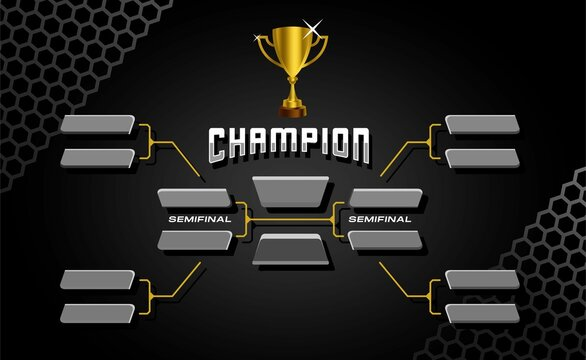
\includegraphics[width=0.5\linewidth]{BSZ_kap_14_2026/by_slide/slide_013/BSZ_kap_14_2026_slide_013_asset_02_image3.jpeg}
  \caption{Relativ prestasjonsmåling som turnering: ansatte rangeres mot hverandre -- filtrerer felles sjokk og belønner relativ innsats. (BSZ kap.\ 14, slide 13) [SLIDE]}
\end{figure}

I principal-agent-rammen filtrerer relativ måling støy: la $Q_i = \alpha e_i + \mu_{\text{common}} + \mu_{i, \text{idio}}$. Da har den relative differansen $Q_i - \bar{Q}_{-i}$ ingen $\mu_{\text{common}}$-komponent og er mer informativ om $e_i$ alene. Informativeness-prinsippet sier at optimal kontrakt bør betinges på $Q_i - \bar{Q}_{-i}$, ikke bare $Q_i$. Pris: man overfører $\mu_{i, \text{idio}}$-risiko mens man fjerner $\mu_{\text{common}}$-risiko -- nettoeffekten avhenger av hvor stor andel av total støy som er felles.

\begin{center}
\renewcommand{\arraystretch}{1.2}
\begin{tabular}{@{}p{3.5cm}p{5.0cm}p{5.0cm}@{}}
\toprule
\textbf{Dimensjon} & \textbf{Absolutt} & \textbf{Relativ} \\
\midrule
Filtrerer felles sjokk? & Nei & Ja \\
Risikopremie & Høyere & Lavere \\
Insentivkoeffisient $\beta$ & Lavere (av risiko) & Kan settes høyere \\
Samarbeidseffekt & Positiv/nøytral & Negativ (sabotasje) \\
Ratchet-fare & Høy & Lav (avhenger ikke av egen historikk) \\
Enkel å kommunisere & Ja & Nei (sammenligningsgrunnlag) \\
\bottomrule
\end{tabular}
\end{center}
[SLIDE/BOK]

\subsection*{Eksempler}
\begin{itemize}
\item \textbf{Equinor LTI (NO).} En vesentlig andel av langtidsprogrammet er knyttet til \emph{relative Total Shareholder Return} (rTSR) mot en peer-gruppe av integrerte oljeselskaper (Shell, BP, TotalEnergies, m.fl.). Dette filtrerer bort oljepris-sjokk som ledelsen ikke kontrollerer. [EKS]
\item \textbf{Microsoft stack ranking (før 2013).} Tvungen relativ rangering der bunn-10\,\% ble vurdert ut. Skapte interne kamper, sabotasje og kunnskapshamstring. Avskaffet i 2013 til fordel for mer absolutt + subjektiv vurdering. [EKS]
\item \textbf{GE Jack Welch ``vitality curve''.} Klassisk relativ rangering 20-70-10. Lik kritikk som Microsoft. [EKS]
\item \textbf{Norske banker, kredittsalg.} Salgskvoter er typisk absolutte (selg N produkter), men toppledelsens bonus knyttes til rTSR mot DNB/Nordea/SEB-peer-gruppen. [EKS]
\item \textbf{Tournaments i akademia.} Stipendiatkonkurranse er relativ -- man får stipend basert på rangering mot medsøkere, ikke en absolutt terskel. [EKS]
\item \textbf{Mærsk PtX-benchmarking.} Sammenligning av prosjektytelse mot Ørsted, Air Liquide og andre PtX-aktører filtrerer bort bransje-/elprissjokk og isolerer prosjektledernes reelle bidrag. [CASE]
\end{itemize}

\subsection*{Kobling til søyle og andre teorier}
Søyle: \STwo\ (måletype) primært, kobler direkte til \SThree\ (bonusberegning). Relaterte teorier: \thref{performance-measurement-purposes}{Formålene med prestasjonsmåling}, \thref{informativeness-principle}{Informativeness-prinsippet} (teoretisk grunnlag), \thref{controllability-principle}{Controllability-prinsippet} (samme motivasjon: filtrer ut ikke-kontrollerbart), \thref{ratchet-effect}{Ratchet-effekten} (relativ er løsning), \thref{gaming-in-performance-measurement}{Gaming}, \thref{subjective-vs-objective-performance}{Subjektiv vs.\ objektiv prestasjonsmåling}, \thref{principal-agent}{Principal-Agent}, \thref{moral-hazard}{Moral hazard}, \thref{agency-costs}{Agency costs}, \thref{incentive-coefficient}{Insentivkoeffisient}.

\paragraph{Brukt i spørsmål:} Q10, Q14.

% !TEX root = ../main.tex
\section{Subjektiv vs.\ objektiv prestasjonsmåling}\label{thr:subjective-vs-objective-performance}

\paragraph{Definisjon.} \emph{Objektiv} prestasjonsmåling bygger på forhåndsdefinerte, kvantifiserbare og verifiserbare kriterier som er fastsatt før perioden starter (salgstall, ROA, prosjektmilestones, kvalitetsindikatorer). \emph{Subjektiv} prestasjonsmåling er en helhetsvurdering som evaluator (typisk linjeleder) foretar etter perioden, og som ofte fanger opp dimensjoner som er vanskelige å kvantifisere -- samarbeid, lederskap, kreativitet, mentoring. [SLIDE]

\subsection*{Forklaring}

Det fundamentale problemet er at de fleste jobber er multidimensjonale, men bare noen dimensjoner kan måles billig og verifiserbart. Den klassiske advarselen er ``you get what you measure'': sett en bonus på salgstall, og selgerne presser dårlige produkter på kunder. Sett en bonus på antall publikasjoner, og forskere splitter forskningen i ``minimum publishable units''. Subjektiv evaluering er BSZs svar på dette: en evaluator kan se hele jobben, inkludert det som ikke lar seg telle, og kan ex post overstyre formelle målinger. [SLIDE]

Men subjektiv evaluering er ikke gratis. Den introduserer en ny prinsipal-agent-relasjon -- mellom selskapet og evaluator -- og fører til \emph{påvirkningskostnader} (Milgrom \& Roberts 1988): ansatte bruker tid på å påvirke evaluatoren sin i stedet for å skape verdi. Den åpner også for partiskhet, og for \emph{supervisor shirking}: lederen unngår å gi ærlige negative vurderinger fordi det skaper konflikt -- alle får ``meets expectations'' uavhengig av reell prestasjon. [SLIDE/BOK]

Løsningen er nesten alltid en \emph{hybrid}: en objektiv komponent (verifiserbar, juridisk holdbar) kombinert med en subjektiv komponent (kvalitativ overstyring, kalibrering på tvers av team). En \emph{bonusbank} der utbetalingen kan justeres senere, og en \emph{kalibreringsprosess} der ledere må forklare og forsvare sine vurderinger overfor hverandre, demper ulempene ved subjektivitet. [BOK]

\subsection*{Kjerneforutsetninger}
\begin{itemize}
\item For \emph{objektiv}: måltallet må være verifiserbart, vanskelig å manipulere, og dekke en stor nok del av den verdiskapende atferden.
\item For \emph{objektiv}: jobben må kunne fanges meningsfullt i ett eller få kvantifiserbare mål -- bryter sammen ved sterk multitasking.
\item For \emph{subjektiv}: evaluator må ha innsikt, tilstrekkelig kompetanse og motivasjon til å gi ærlige vurderinger.
\item For \emph{subjektiv}: organisasjonen må ha mekanismer (kalibrering, peer review) som demper bias og supervisor shirking.
\item Tillit mellom evaluator og evaluert -- ellers kollapser informasjonsverdien av subjektive vurderinger.
\item Kontraktsrettslig: subjektive evalueringer er vanskeligere å forsvare i arbeidsrettslige tvister enn objektive.
\end{itemize}

\subsection*{Muligheter (når hver type bør velges)}
\begin{itemize}
\item \textbf{Objektiv} foretrukket når: jobben er énledimensjonal og lett målbar (salg, produksjon, akkord); tillit mellom ledelse og ansatte er lav; det er behov for transparente og rettferdige rangeringer.
\item \textbf{Subjektiv} foretrukket når: jobben er multidimensjonal (lederskap, FoU, kreative profesjoner); samarbeid og mentoring er kritisk; selskapets verdiskaping ligger i \emph{hvordan} arbeidet gjøres, ikke bare \emph{hvor mye}.
\item \textbf{Hybrid} foretrukket nesten alltid for ledere: objektiv formel + subjektiv overstyring fanger det målbare uten å miste det viktige.
\item Subjektiv evaluering kan dempe \thref{gaming-in-performance-measurement}{gaming} -- en evaluator ser at salgstallene er pyntet, eller at OPEX er kjørt ned på bekostning av vedlikehold.
\item Subjektiv evaluering kan dempe \thref{ratchet-effect}{ratchet-effekten} -- evaluatoren kan velge å ikke straffe overprestasjon med strammere fremtidsmål.
\end{itemize}

\subsection*{Begrensninger og kritikk}
\begin{itemize}
\item \textbf{Objektiv: imperfekt proxy.} Måler bare det målbare; lar resten av jobben være ubelønnet. Skaper gaming og multitasking-vridninger.
\item \textbf{Objektiv: rigid.} Når omgivelsene endrer seg midt i perioden, kan målet bli irrelevant eller umulig -- demotiverende.
\item \textbf{Objektiv: lett å gamble.} Verifiserbart betyr at agenten vet nøyaktig hvilken atferd som betaler seg -- og kan optimere mot \emph{målet} fremfor mot verdien.
\item \textbf{Subjektiv: påvirkningskostnader.} Ansatte bruker tid på selvpromotering, nettverksbygging mot evaluator, og på å posisjonere seg i kalibreringsmøter.
\item \textbf{Subjektiv: bias og diskriminering.} Empirisk dokumentert at subjektive evalueringer systematisk straffer kvinner, minoriteter og folk som ikke ligner evaluatoren.
\item \textbf{Subjektiv: supervisor shirking.} Det er ubehagelig å gi negative vurderinger -- alle får ``OK'', distribusjonen kollapser, signalverdien forsvinner. Motiveringen for \emph{forced distribution} (men den har egne ulemper).
\item \textbf{Subjektiv: juridisk sårbarhet.} I norske arbeidsforhold må oppsigelse og sterkt ulik lønn kunne dokumenteres -- ren subjektivitet er ikke holdbar i en konfliktsak.
\item \textbf{Hybrid:} Krever klar vekting, kalibreringsdisiplin og tillit; bryter sammen i selskaper med svak HR-funksjon.
\end{itemize}

\subsection*{Modell / illustrasjon}

I principal-agent-rammen kan kompensasjonen skrives som
\[ W = W_0 + \beta_O \cdot Q_O + \beta_S \cdot S \]
der $Q_O$ er det objektive utfallet og $S$ er evaluatorens subjektive score. Optimal vekting $\beta_O$ vs.\ $\beta_S$ avhenger av (a) informasjonsinnholdet i hvert mål om innsats, (b) påvirkningskostnaden $S$ åpner for, og (c) tilliten til evaluator. Når $Q_O$ er en god proxy, dominerer den; når jobben er multidimensjonal, må $\beta_S > 0$. [BOK]

\begin{center}
\renewcommand{\arraystretch}{1.2}
\begin{tabular}{@{}p{3.0cm}p{5.0cm}p{5.0cm}@{}}
\toprule
\textbf{Dimensjon} & \textbf{Objektiv} & \textbf{Subjektiv} \\
\midrule
Verifiserbarhet & Høy & Lav \\
Gaming-risiko & Høy & Lav (evaluator ser) \\
Multitasking-dekning & Lav & Høy \\
Påvirkningskostnader & Lave & Høye \\
Bias-risiko & Lav & Høy \\
Juridisk holdbarhet & Høy & Lav \\
Tillit som krav & Liten & Stor \\
\bottomrule
\end{tabular}
\end{center}
[SLIDE]

\subsection*{Eksempler}
\begin{itemize}
\item \textbf{McKinsey \& Co.\ partnerevaluering.} Tungt subjektiv -- kolleger og partnere vurderer på dimensjoner som klientimpact, mentoring, firmaets verdier. Få objektive måltall direkte koblet til lønn. Krever sterk kalibreringsdisiplin og er kostbar å administrere, men passer en multidimensjonal kunnskapsjobb. [EKS]
\item \textbf{Wells Fargo (US, 2016).} Ekstremt objektiv kompensasjon: bonus per kryssolgt produkt. Resultatet var 3,5 mill.\ falske kontoer -- en katastrofal gaming-historie. Etter skandalen lagt om til mer subjektiv balansert evaluering. [EKS]
\item \textbf{Microsoft (post-2013).} Avskaffet stack ranking (objektivt distribusjons-system) til fordel for ``Connect''-samtaler -- mer subjektiv, holistisk evaluering. Konkret eksempel på pendelsvingning fra objektiv til mer subjektiv. [EKS]
\item \textbf{DNB rådgivere (NO, 2010-tallet).} Provisjonsbasert objektiv måling skapte gaming (anbefale dyre fond). Endret til hybrid med subjektiv kvalitetsvurdering av kundeanbefalinger. [EKS]
\item \textbf{Norske akademiske ansettelser.} Hybrid: objektive publikasjonsmål (tellekantsystem) + subjektiv bedømmelsekomité. Tellekantsystemet alene utløste gaming (salami-publikasjoner), så komiteen er motvekt. [EKS]
\item \textbf{Mærsk PtX prosjektledelse.} Objektive milestones (FID, kontrakter signert, anlegg ferdig) + subjektiv vurdering av partnerkvalitet, sikkerhetskultur og teknologivalg ratifisert av Decision Control. [CASE]
\end{itemize}

\subsection*{Kobling til søyle og andre teorier}
Søyle: \STwo\ (måletype) primært, kobler til \SThree\ (utbetalingsformel) og \SOne\ (hvem som skal evaluere -- decision control). Relaterte teorier: \thref{performance-measurement-purposes}{Formålene med prestasjonsmåling}, \thref{gaming-in-performance-measurement}{Gaming}, \thref{ratchet-effect}{Ratchet-effekten}, \thref{absolute-vs-relative-performance}{Absolutt vs.\ relativ prestasjonsmåling}, \thref{informativeness-principle}{Informativeness-prinsippet}, \thref{controllability-principle}{Controllability-prinsippet}, \thref{principal-agent}{Principal-Agent}, \thref{moral-hazard}{Moral hazard}, \thref{agency-costs}{Agency costs}, \thref{decision-management-control}{Decision Management vs.\ Decision Control}, \thref{incentive-coefficient}{Insentivkoeffisient}.

\paragraph{Brukt i spørsmål:} Q10.

% Q11 theories
% !TEX root = ../main.tex
\section{Boundaries of the Firm}\label{thr:boundaries-of-the-firm}

\paragraph{Definisjon.} \emph{Boundaries of the Firm} refererer til spørsmålet om hvilke aktiviteter som bør foregå \emph{innenfor} firmaet (make) versus anskaffes via \emph{markedstransaksjoner} (buy). Grensene bestemmes av den relative størrelsen på transaksjonskostnader i markedet sammenlignet med byråkratikostnader internt (Coase 1937). [SLIDE]

\subsection*{Forklaring}

BSZ kap.\ 8/19 presenterer firmaet som et \emph{nexus of contracts} -- en knute av kontrakter mellom input-eiere (arbeidere, kapitalgivere, leverandører). Firmaets grenser er ikke gitt av teknologi, men av \emph{organisatoriske valg}. To hovedperspektiver: [SLIDE/BOK]

\textbf{1. Coase (1937) -- transaksjonskostnader.} Markedet koordinerer via priser, men det koster å bruke prismekanismen: søke-/informasjonskostnader, forhandlingskostnader, kontraktskrivning og håndhevelse. Firmaet erstatter markedstransaksjoner med hierarkisk styring. Firmaets grense trekkes der \emph{marginal intern organiseringskostnad} = \emph{marginal transaksjonskostnad i markedet}. [BOK]

\textbf{2. Williamson (1979/1985) -- transaksjonsspesifikke aktiva.} Coases rammeverk utvides: grensene avhenger av tre transaksjonsegenskaper: (i) \emph{asset specificity} (investering med lav alternativverdi), (ii) \emph{uncertainty} (vanskeligheten av å forutse kontraktstilstander), (iii) \emph{frequency} (gjentakelse senker per-enhet-styringskostnader internt). Høy aktivaspesifisitet + høy usikkerhet $\Rightarrow$ \thref{costly-contracting}{costly contracting} og \thref{hold-up-problem}{hold-up-risiko} $\Rightarrow$ vertikal integrasjon lønner seg. [BOK]

\textbf{3. Eierskap av produktionsfaktorer.} BSZ kap.\ 8 understreker at \emph{hvem som eier de kritiske produktionsfaktorene} bestemmer hvem som har \emph{residuelle beslutningsrettigheter} i tilstander kontrakten ikke dekker (Grossman--Hart--Moore). Eierskap = kontrollrett når kontrakten er stille. Vertikal integrasjon overfører eierskap (og dermed kontroll) av oppstrøms- eller nedstrømsaktiva til firmaet. [SLIDE]

\textbf{Regnskapsmessig vs.\ økonomisk profit} er en nødvendig sondring for å vurdere om en aktivitet reelt sett skaper verdier innenfor firmaets grenser eller om den burde outsources. Regnskapet viser positive marginer, men når alternativkostnaden (opportunity cost) inkluderes, kan aktiviteten ha negativ \emph{økonomisk} profit -- da bør den flyttes utenfor firmaet. Se \thref{accounting-vs-economic-profit}{accounting vs.\ economic profit}. [SLIDE]

\subsection*{Kjerneforutsetninger}
\begin{itemize}
\item Kontrakter er \emph{ufullstendige} (\thref{costly-contracting}{costly contracting}).
\item Rasjonelle aktører som optimerer -- men med begrenset rasjonalitet (Simon).
\item Opportunisme: aktører utnytter kontraktshull og informasjonsasymmetri.
\item Transaksjonskostnader er sammenlignbare på tvers av alternativer (make vs.\ buy).
\item Eierskap gir residuell kontrollrett (Grossman--Hart--Moore).
\end{itemize}

\subsection*{Muligheter}
\begin{itemize}
\item Forklarer \emph{hvorfor firmaer eksisterer} -- de er en alternativ styringsform til markedet.
\item Predikerer når vertikal integrasjon er effektivt (høy asset specificity, høy usikkerhet).
\item Gir et normativt rammeverk for \emph{make-or-buy}-beslutninger.
\item Kobler eierskap til insentiver: eierskap av aktiva justerer holdout-makt og insentiver til relasjonsspesifikke investeringer.
\end{itemize}

\subsection*{Begrensninger og kritikk}
\begin{itemize}
\item Transaksjonskostnader er vanskelige å måle empirisk -- modellen gir retning men sjelden presise tall.
\item Ignorerer langsiktige relasjoner og tillitsbasert samarbeid som kan fungere uten formell integrasjon (japanske keiretsu, skandinaviske leverandørnettverk).
\item Underestimerer byråkratikostnader internt -- vertikal integrasjon bringer egne agentkostnader.
\item Grossman--Hart--Moore-modellen forutsetter at eierskap er binært; i praksis finnes mellomformer (JV, minoritetseierskap, franchising).
\item Fokuserer på effektivitet og ignorerer strategiske motiver (market power, entry deterrence).
\end{itemize}

\subsection*{Modell / illustrasjon}

\begin{figure}[H]
  \centering
  
\includegraphics[width=0.6\linewidth]{BSZ_kap_8_2026/by_slide/slide_002/BSZ_kap_8_2026_slide_002_asset_01_image1.jpeg}
  \caption{Firmaets grenser: strategiske valg om hva som skal gjøres internt (make) vs.\ eksternt (buy) -- et nettverk av kontraktsrelasjoner. (BSZ kap.\ 8, slide 2) [SLIDE]}
\end{figure}

\begin{center}
\renewcommand{\arraystretch}{1.15}
\begin{tabular}{@{}p{3.5cm}p{5cm}p{5.5cm}@{}}
\toprule
\textbf{Faktor} & \textbf{Favoriserer marked (buy)} & \textbf{Favoriserer firma (make)} \\
\midrule
Asset specificity & Lav (generelle aktiva) & Høy (spesifikke aktiva) \\
Usikkerhet & Lav, forutsigbar & Høy, vanskelig å kontrahere \\
Frekvens & Sjelden/engangs & Hyppig/gjentakende \\
Målbarhet & Output lett verifiserbart & Output vanskelig verifiserbart \\
Marked finnes? & Konkurrerende leverandørmarked & Fåtall/monopol leverandør \\
\bottomrule
\end{tabular}
\end{center}
\textit{Tabell: Williamsons transaksjonsegenskaper og valg av styringsform. [BOK]}

\subsection*{Eksempler}
\begin{itemize}\setlength{\itemsep}{2pt}
\item \textbf{Toyota vs.\ GM.} Toyota holdt leverandørene utenfor firmaets grenser, men brukte langsiktige relasjoner, JIT og delt produktutvikling som \emph{hybrider} mellom marked og hierarki. GM vertikalt integrerte massive deleoperasjoner (Fisher Body), delvis grunnet hold-up-faren ved spesifikke pressverktøy. [EKS]
\item \textbf{Mærsk og terminal-operasjoner.} Mærsk eier APM Terminals og integrerte nedstrøms for å kontrollere havnekapasitet -- et svært spesifikt aktivum med høy usikkerhet og store sunk costs. Andre rederier (Hapag-Lloyd) outsourcer terminal og bruker tredjepartsoperatører. [EKS]
\end{itemize}

\subsection*{Kobling til søyle og andre teorier}
Søyle: \SOne\ (hvem har beslutningsrett over hvilke aktiviteter). Relaterte: \thref{costly-contracting}{Costly contracting}, \thref{specific-vs-general-knowledge}{Spesifik vs.\ generell viden}, \thref{agency-costs}{Agency costs}, \thref{vertical-integration-outsourcing}{Vertikal integrasjon og outsourcing}, \thref{hold-up-problem}{Hold-up-problemet}, \thref{accounting-vs-economic-profit}{Accounting vs.\ economic profit}.

\paragraph{Brukt i spørsmål:} Q11, Q12.

% !TEX root = ../main.tex
\section{Accounting vs.\ Economic Profit}\label{thr:accounting-vs-economic-profit}

\paragraph{Definisjon.} \emph{Regnskabsmæssig profit} (accounting profit) er inntekter minus eksplisitte bokførte kostnader. \emph{Økonomisk profit} (economic profit) er inntekter minus \emph{alle} kostnader, inkludert \emph{opportunity costs} -- verdien av den beste alternative bruken av ressursene. En aktivitet med positiv regnskapsprofitt kan ha negativ økonomisk profitt hvis alternativkostnaden overstiger regnskapsmarginen. [SLIDE]

\subsection*{Forklaring}

BSZ kap.\ 8 bruker distinksjonen til å forklare to ting: [SLIDE]

\textbf{1. Korrekt beslutningsgrunnlag.} Ledere som kun ser på regnskapstall kan beholde aktiviteter som \emph{ødelegger verdi} fordi de ignorerer alternativkostnaden. Økonomisk profitt er det riktige beslutningskriteriet -- det fanger den reelle verdiskapningen utover hva ressursene ville tjent i sin beste alternative anvendelse. [BOK]

\textbf{2. Boundaries of the Firm.} Hvis en vertikal integrert enhet viser positiv regnskapsprofitt men negativ økonomisk profitt, bør aktiviteten \emph{outsources}: markedet kan utføre den billigere. Eksemplet er et oljeselskap som raffinerer selv -- raffineringsmarginene dekker regnskapskostnadene, men opportunity-kosten ved å binde kapital i et raffineri (i stedet for å reinvestere i leting) gjør at økonomisk profitt er negativ. [SLIDE]

\textbf{Formell sondring:}
\[
\pi_{\text{accounting}} = R - C_{\text{explicit}}, \qquad
\pi_{\text{economic}} = R - C_{\text{explicit}} - C_{\text{opportunity}}
\]
Forskjellen, $C_{\text{opportunity}}$, inkluderer: (i) alternativ avkastning på investert kapital, (ii) verdi av eierens tid/kompetanse i annen anvendelse, (iii) alternativ salgspris for innsatsfaktorer i markedet. [BOK]

\subsection*{Kjerneforutsetninger}
\begin{itemize}
\item Et velfungerende marked eksisterer for innsatsfaktorene, slik at opportunity cost kan prises.
\item Ledere har (eller bør ha) informasjon om alternativavkastning.
\item Regnskapssystemet dekker eksplisitte kostnader korrekt (avskrivninger, renter, lønninger).
\end{itemize}

\subsection*{Muligheter}
\begin{itemize}
\item Avslører om vertikal integrasjon faktisk skaper verdi eller bare maskerer dårlige alternativer.
\item Gir normativt kriterium for \emph{make-or-buy}: outsource hvis $\pi_{\text{economic}}<0$.
\item Kobler til EVA/residual income-modeller i \thref{responsibility-centers}{investment centers}.
\end{itemize}

\subsection*{Begrensninger og kritikk}
\begin{itemize}
\item Opportunity cost er vanskelig å estimere presist -- avhenger av kontrafaktiske scenarioer.
\item I fravær av likvide markeder (f.eks.\ for spesifikke aktiva) er alternativverdien uklar.
\item Regnskapsprofitten er det eneste som rapporteres eksternt; økonomisk profitt krever intern analyse.
\item Strategiske hensyn (kontroll, sikkerhet, market power) kan rettferdiggjøre aktiviteter med negativ $\pi_{\text{economic}}$ -- modellen er nødvendig men ikke tilstrekkelig.
\end{itemize}

\subsection*{Modell / illustrasjon}

\begin{figure}[H]
  \centering
  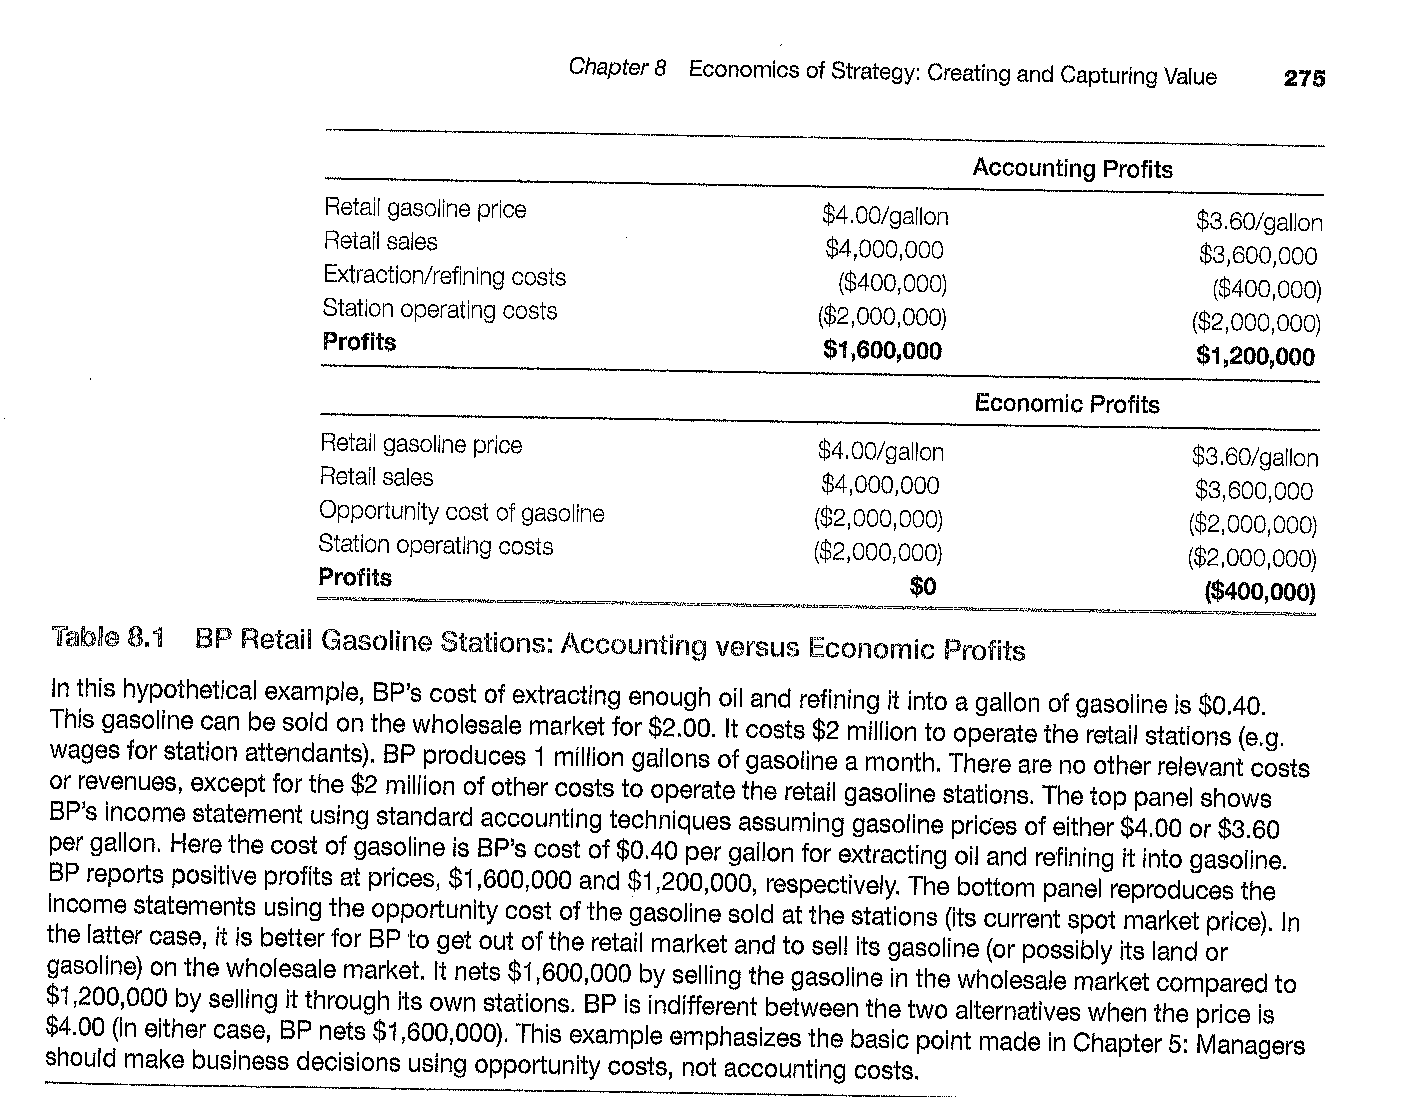
\includegraphics[width=0.7\linewidth]{BSZ_kap_8_2026/by_slide/slide_011/BSZ_kap_8_2026_slide_011_asset_01_image6.png}
  \caption{BP Retail Gasoline Stations: regnskapsmessig vs.\ økonomisk profitt. Ved \$3{,}60/gallon er regnskapsmessig profitt positiv (\$1{,}2M) men økonomisk profitt negativ (-\$400k) fordi opportunity cost for bensin solgt i eget nettverk overstiger marginen. Eksemplet viser at BP bør outsource/selge detaljistoperasjonen. [SLIDE -- BSZ kap.\ 8, Table 8.1]}
\end{figure}

\subsection*{Eksempler}
\begin{itemize}\setlength{\itemsep}{2pt}
\item \textbf{BP gasoline stations (BSZ Table 8.1):} Regnskapsprofitt \$1{,}2M vs.\ økonomisk profitt -\$400k ved lavere bensinpris -- illustrerer at detaljistleddet ødelegger verdi. [SLIDE]
\item \textbf{Norsk kommune og egen IT-drift:} Kommunen viser lave IT-kostnader i regnskapet, men inkluderer ikke alternativkostnaden av IT-personalets tid og kommunens forhandlingsmakt i et konkurranseutsatt marked. Outsourcing kan gi positiv økonomisk profitt selv om regnskapskostnadene stiger. [EKS]
\end{itemize}

\subsection*{Kobling til søyle og andre teorier}
Søyle: \STwo\ (korrekt prestasjonsmåling krever riktig profittbegrep). Relaterte: \thref{boundaries-of-the-firm}{Boundaries of the Firm}, \thref{responsibility-centers}{Responsibility centers} (EVA i investment centers), \thref{transfer-pricing}{Transfer pricing} (intern prising reflekterer opportunity cost), \thref{vertical-integration-outsourcing}{Vertikal integrasjon og outsourcing}.

\paragraph{Brukt i spørsmål:} Q11.

% !TEX root = ../main.tex
\section{Vertikal integrasjon og outsourcing}\label{thr:vertical-integration-outsourcing}

\paragraph{Definisjon.} \emph{Vertikal integrasjon} innebærer at et firma tar eierskap over aktiviteter i tilstøtende ledd i verdikjeden (oppstrøms leverandører eller nedstrøms distribusjon). \emph{Outsourcing} (market transactions) innebærer at disse aktivitetene anskaffes via kontrakter med uavhengige markedsaktører. Valget er en kjernebeslutning i \thref{boundaries-of-the-firm}{Boundaries of the Firm}. [SLIDE]

\subsection*{Forklaring}

BSZ kap.\ 8/19 diskuterer make-or-buy-beslutningen langs tre dimensjoner: transaksjonskostnader, insentiver og markedsmakt. [SLIDE]

\textbf{Fordeler ved outsourcing (markedstransaksjoner):}
\begin{enumerate}\setlength{\itemsep}{2pt}
\item \textbf{Markedsdisiplin og prismekanisme.} Konkurranseeksponering tvinger leverandøren til kostnadseffektivitet -- interne enheter mangler dette presset. [SLIDE]
\item \textbf{Spesialisering og skalafordeler.} Ekstern leverandør betjener mange kunder og oppnår stordriftsfordeler firmaet selv ikke kan matche. [SLIDE]
\item \textbf{Fleksibilitet.} Lettere å bytte leverandør enn å omstrukturere intern produksjon ved endret etterspørsel. [BOK]
\item \textbf{Sterkere insentiver.} Leverandøren er \emph{residual claimant} på sin profitt, mens en intern enhet typisk kompenseres med svakere insentiver (cost center). Jf.\ \thref{residual-claimants}{residual claimants}. [SLIDE]
\item \textbf{Unngå byråkratikostnader.} Hierarkisk styring bringer koordinasjon, monitoring og politiske kostnader som markedskontrakter slipper. [BOK]
\end{enumerate}

\textbf{Ulemper ved outsourcing (fordeler ved vertikal integrasjon):}
\begin{enumerate}\setlength{\itemsep}{2pt}
\item \textbf{Transaksjonskostnader.} Søke-, forhandlings-, overvåknings- og håndhevingskostnader kan overstige interne styringskostnader -- særlig ved \emph{spesifikke aktiva}. Jf.\ \thref{costly-contracting}{costly contracting}. [SLIDE]
\item \textbf{Hold-up-problemet.} Når relasjonen krever spesifikke investeringer, risikerer parten med svakest forhandlingsposisjon at motparten reforhandler ex post. Integrasjon eliminerer hold-up. Se \thref{hold-up-problem}{hold-up-problemet}. [SLIDE]
\item \textbf{Free-rider-problemet.} Uavhengige distributører kan underinvestere i service/merkevare fordi gevinsten deles med andre. Integrasjon internaliserer eksternaliteten. Se \thref{free-rider-problem}{free-rider-problemet}. [BOK]
\item \textbf{Double markup.} Når to suksessive monopolister priser uavhengig, blir sluttprisen for høy og kvantum for lavt -- vertikal integrasjon fjerner den ene markupen. Se \thref{double-markup-problem}{double markup-problemet}. [SLIDE]
\item \textbf{Koordinasjon og informasjonsflyt.} Intern koordinasjon kan være enklere enn å formidle \thref{specific-vs-general-knowledge}{spesifikk viten} via prismekanismen. [BOK]
\item \textbf{Beskyttelse av immaterielle rettigheter.} Outsourcing krever deling av teknologi/prosesser -- integrasjon beskytter trade secrets. [BOK]
\item \textbf{Market power.} VI kan brukes strategisk for å kontrollere tilgang til inputs eller distribusjon -- se \thref{vertical-integration-market-power}{VI og market power}. [SLIDE]
\end{enumerate}

\subsection*{Kjerneforutsetninger}
\begin{itemize}
\item Make-or-buy er et dikotomt valg (i praksis finnes mellomformer: franchising, JV, allianse).
\item Transaksjonskostnader og byråkratikostnader er sammenlignbare.
\item Kontraktsufullstendighet er grunnen til at markedet feiler -- med \thref{costless-contracting}{costless contracting} ville outsourcing alltid dominert.
\item Firmaets interne organisasjon er \emph{ikke} gratis -- agentkostnader internt erstatter transaksjonskostnader i markedet.
\end{itemize}

\subsection*{Muligheter}
\begin{itemize}
\item Forklarer verdikjedebeslutninger i de fleste industrier (bilindustri, energi, teknologi, shipping).
\item Predikerer outsourcing-trenden: når teknologi senker søke-/transaksjonskostnader (digitale plattformer, standardisering), øker outsourcing.
\item Predikerer integrasjon ved: høy asset specificity, dårlig leverandørmarked, store eksternaliteter.
\end{itemize}

\subsection*{Begrensninger og kritikk}
\begin{itemize}
\item Mellomformer (franchising, joint ventures, strategiske allianser) passer ikke ren dikotomi.
\item Ignorerer dynamikk: integrasjon i dag kan bli en byrde i morgen (lock-in i vertikal struktur).
\item Kulturelle og ledelsesmessige kapasitetshensyn: integrasjon krever lederkompetanse i nye verdikjedeledd.
\item Strategiske/politiske motiver (nasjonalt eierskap, regulering) overstyrer transaksjonskostnadsvurdering.
\end{itemize}

\subsection*{Modell / illustrasjon}

\begin{figure}[H]
  \centering
  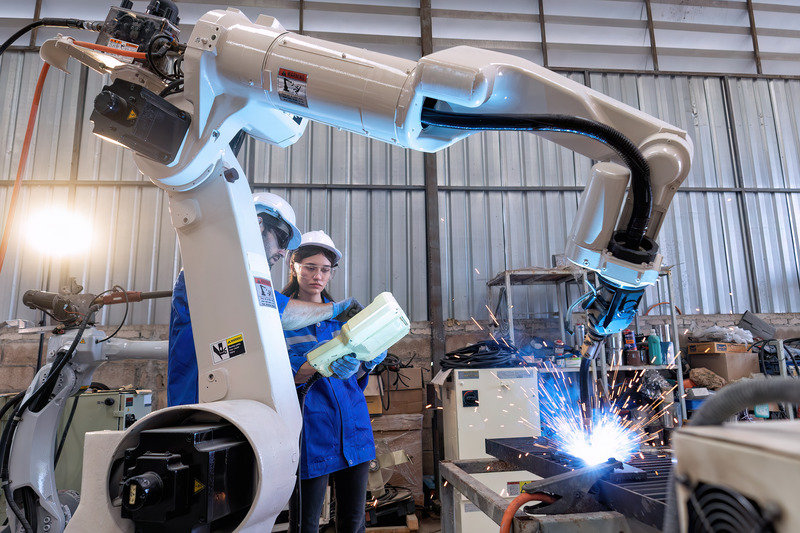
\includegraphics[width=0.5\linewidth]{BSZ_kap_8_2026/by_slide/slide_009/BSZ_kap_8_2026_slide_009_asset_02_image5.jpeg}
  \caption{Spesialisert produksjonsutstyr (robotarm-fabrikk): make-or-buy-beslutningen avhenger av aktivaspesifisitet -- jo mer relasjonsspesifik investering, desto sterkere argument for vertikal integrasjon for å redusere hold-up-risiko og transaksjonskostnader. (BSZ kap.\ 8, slide 9) [SLIDE]}
\end{figure}

\begin{center}
\renewcommand{\arraystretch}{1.15}
\begin{tabular}{@{}p{4.0cm}p{5.0cm}p{5.0cm}@{}}
\toprule
 & \textbf{Vertikal integrasjon (make)} & \textbf{Outsourcing (buy)} \\
\midrule
Transaksjonskostnader & Lave (intern styring) & Kan være høye (søk, forhandling, håndhevelse) \\
Byråkratikostnader & Kan være høye (hierarki) & Lave (markedsdisiplin) \\
Insentiver & Svakere (\thref{agency-costs}{agency costs}) & Sterkere (residual claimant) \\
Fleksibilitet & Lav (lock-in i kapasitet) & Høy (bytte leverandør) \\
Koordinasjon & Direkte styring & Via kontrakt/pris \\
Hold-up-risiko & Eliminert & Kritisk ved spesifikke aktiva \\
Market power & Mulig (kontroll verdikjede) & Begrenset \\
\bottomrule
\end{tabular}
\end{center}
\textit{Tabell: Sammenligning av vertikal integrasjon og outsourcing langs sentrale dimensjoner. [SLIDE/BOK]}

\subsection*{Eksempler}
\begin{itemize}\setlength{\itemsep}{2pt}
\item \textbf{Apple (outsourcing + kontroll):} Apple designer selv (integrert) men produserer hos Foxconn/TSMC (outsourcet). Fordi chip-design er svært spesifikt men produksjonsteknologi er standardisert, har Apple valgt en hybrid: eierskap til IP, markedskontrakt for produksjon. [EKS]
\item \textbf{Equinor og brønnservice:} Equinor outsourcer brønntjenester (Schlumberger, Halliburton) fordi kompetansen er generell og leverandørmarkedet er konkurrerende. Men feltspesifikt utstyr kan skape hold-up -- løst med flerårige rammeavtaler med opsjonsklausuler. [EKS]
\item \textbf{Mærsk og APM Terminals:} Mærsk integrerte nedstrøms i terminal-operasjoner for å sikre havnekapasitet -- et \emph{bottleneck}-aktivum med høy spesifisitet. [CASE]
\end{itemize}

\subsection*{Kobling til søyle og andre teorier}
Søyle: \SOne\ (beslutningsrett over verdikjedeledd), \SThree\ (insentivdesign for interne vs.\ eksterne enheter). Relaterte: \thref{boundaries-of-the-firm}{Boundaries of the Firm}, \thref{costly-contracting}{Costly contracting}, \thref{hold-up-problem}{Hold-up-problemet}, \thref{free-rider-problem}{Free-rider-problemet}, \thref{double-markup-problem}{Double markup-problemet}, \thref{vertical-integration-market-power}{VI og market power}, \thref{agency-costs}{Agency costs}, \thref{specific-vs-general-knowledge}{Spesifik vs.\ generell viden}, \thref{transfer-pricing}{Transfer pricing}, \thref{accounting-vs-economic-profit}{Accounting vs.\ economic profit}.

\paragraph{Brukt i spørsmål:} Q11, Q12.

% !TEX root = ../main.tex
\section{Vertikal integrasjon og market power}\label{thr:vertical-integration-market-power}

\paragraph{Definisjon.} Vertikal integrasjon kan brukes som et \emph{strategisk instrument} til å oppnå markedsmakt ved å kontrollere tilgang til essensielle inputs (oppstrøms) eller distribusjonskanaler (nedstrøms), og dermed stenge ute konkurrenter eller øke switching costs. BSZ kap.\ 19 presenterer modellen som viser hvordan en integrert produsent kan monopolisere nedstrømsmarkedet gjennom kontroll av et kritisk oppstrøms-input. [SLIDE]

\subsection*{Forklaring}

\textbf{Mekanismen.} Anta at en oppstrøms produsent $U$ er eneste kilde til et kritisk input. $U$ integrerer fremover (kjøper nedstrømsbedrift $D_1$). Nå kontrollerer $U$--$D_1$ tilgangen til input for rivaliserende nedstrømsaktører $D_2, D_3, \ldots$. $U$--$D_1$ kan: [SLIDE/BOK]

\begin{enumerate}\setlength{\itemsep}{2pt}
\item \textbf{Foreclosure:} Nekte å selge input til $D_2$, $D_3$ (eller sette prohibitiv pris) -- konkurrentene presses ut av markedet.
\item \textbf{Raising rivals' costs:} Selge input til $D_2$ til en høyere pris enn interne $D_1$ betaler -- $D_2$ taper kostnadskonkurranse.
\item \textbf{Kontroll av flaskehals:} Eierskap til infrastruktur (havn, rørledning, nett) gir gatekeeper-makt.
\end{enumerate}

\textbf{Resultat:} Nedstrømsmarkedet beveger seg mot monopol/duopol; sluttforbrukerpris stiger, kvantum synker, samfunnsmessig dødvektstap oppstår. Dette er et \emph{konkurranserettslig} problem -- regulering eller kartellmyndighet kan gripe inn (jf.\ \thref{market-failure-regulation}{regulering}). [BOK]

\subsection*{Grafisk modell -- vertikal integrasjon for market power}

\begin{figure}[h]
\centering
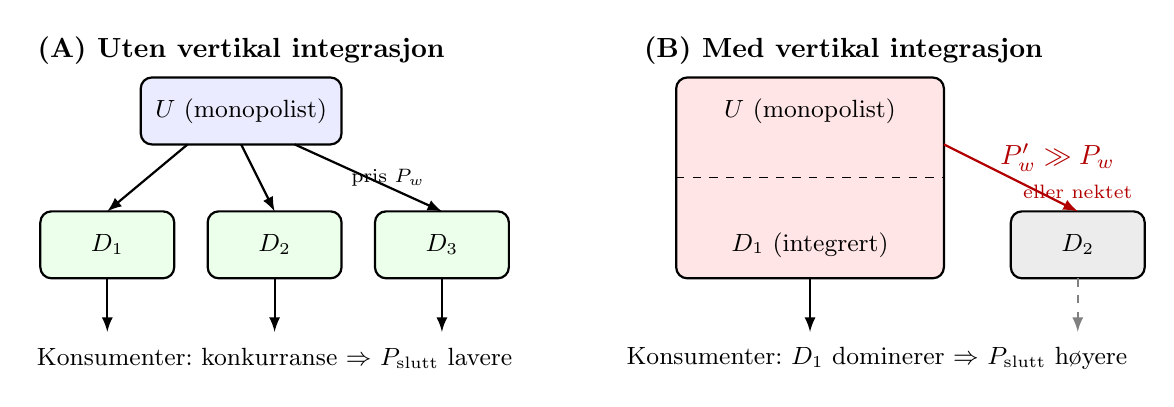
\begin{tikzpicture}[>=latex, scale=0.85, every node/.style={font=\small}]
  % --- Situasjon 1: Uten VI ---
  \node[font=\bfseries] at (3, 7.2) {(A) Uten vertikal integrasjon};
  % Upstream
  \draw[thick, rounded corners, fill=blue!8] (1.5,5.8) rectangle (4.5,6.8);
  \node at (3,6.3) {$U$ (monopolist)};
  % Downstream firms
  \draw[thick, rounded corners, fill=green!8] (0,3.8) rectangle (2,4.8);
  \node at (1,4.3) {$D_1$};
  \draw[thick, rounded corners, fill=green!8] (2.5,3.8) rectangle (4.5,4.8);
  \node at (3.5,4.3) {$D_2$};
  \draw[thick, rounded corners, fill=green!8] (5,3.8) rectangle (7,4.8);
  \node at (6,4.3) {$D_3$};
  % Arrows
  \draw[->, thick] (2.2,5.8) -- (1,4.8);
  \draw[->, thick] (3,5.8) -- (3.5,4.8);
  \draw[->, thick] (3.8,5.8) -- (6,4.8);
  \node[right] at (4.5,5.3) {\scriptsize pris $P_w$};
  % Konsumenter
  \draw[->, thick] (1,3.8) -- (1,3.0);
  \draw[->, thick] (3.5,3.8) -- (3.5,3.0);
  \draw[->, thick] (6,3.8) -- (6,3.0);
  \node at (3.5,2.6) {Konsumenter: konkurranse $\Rightarrow$ $P_{\text{slutt}}$ lavere};

  % --- Situasjon 2: Med VI ---
  \begin{scope}[xshift=9cm]
  \node[font=\bfseries] at (3, 7.2) {(B) Med vertikal integrasjon};
  % Integrert firma
  \draw[thick, rounded corners, fill=red!10] (0.5,3.8) rectangle (4.5,6.8);
  \node at (2.5,6.3) {$U$ (monopolist)};
  \node at (2.5,4.3) {$D_1$ (integrert)};
  \draw[dashed] (0.5,5.3) -- (4.5,5.3);
  % Rivaler
  \draw[thick, rounded corners, fill=gray!15] (5.5,3.8) rectangle (7.5,4.8);
  \node at (6.5,4.3) {$D_2$};
  % Arrow med X
  \draw[->, thick, red!70!black] (4.5,5.8) -- (6.5,4.8);
  \node[red!70!black, font=\bfseries] at (6.2,5.6) {$P_w' \gg P_w$};
  \node[red!70!black, font=\scriptsize] at (6.5,5.1) {eller nektet};
  % Konsumenter
  \draw[->, thick] (2.5,3.8) -- (2.5,3.0);
  \draw[->, thick, dashed, gray] (6.5,3.8) -- (6.5,3.0);
  \node at (3.5,2.6) {Konsumenter: $D_1$ dominerer $\Rightarrow$ $P_{\text{slutt}}$ høyere};
  \end{scope}
\end{tikzpicture}
\caption{\textbf{Vertikal integrasjon for market power.} (A) Uten VI: oppstrøms monopolist $U$ selger til alle nedstrøms-aktører til pris $P_w$; konkurranse blant $D_1$--$D_3$ holder sluttprisen nede. (B) Med VI: $U$--$D_1$ integrert; rivalen $D_2$ nektes input eller betaler prohibitiv pris $P_w'\gg P_w$ (\emph{foreclosure / raising rivals' costs}). $D_1$ får markedsmakt nedstrøms, sluttprisen stiger. [SLIDE/BOK -- BSZ kap.\ 19]}
\end{figure}

\subsection*{Kjerneforutsetninger}
\begin{itemize}
\item Oppstrøms monopol (eller sterk markedsposisjon) -- uten dette kan ikke foreclosure fungere.
\item Nedstrømsmarkedet er imperfekt: rivaler kan ikke skaffe input fra andre kilder.
\item Ingen effektiv regulering som forbyr foreclosure.
\item Integrert firma har incentiv til å begrense konkurranse (profitt fra monopolisering > tap fra redusert upstream-salg til rivaler).
\end{itemize}

\subsection*{Muligheter}
\begin{itemize}
\item Forklarer hvorfor konkurransemyndigheter (EU DG Comp, US DOJ) gjennomgår vertikale fusjoner.
\item Predikerer i hvilke industrier VI gir markedsmakt: flaskehals-industrier (nettverk, infrastruktur, sjeldne råvarer).
\item Gir normativt grunnlag for regulering av nettnøytralitet, tilgang til infrastruktur og essensiell fasilitets-doktrine.
\end{itemize}

\subsection*{Begrensninger og kritikk}
\begin{itemize}
\item Chicago School-kritikken: VI skaper ikke ny monopolmakt -- oppstrømsmonopolisten kan allerede ekstrahere all monopolprofitt via inputpris. VI er da nøytral eller effektivitetsfremmende (eliminerer double markup).
\item Forutsetter at oppstrøms monopol er varig -- entry, innovasjon eller substitutter kan undergrave foreclosure.
\item Reguleringsmyndigheter kan pålegge tilgangsforpliktelser (unbundling, FRAND-lisenser) som gjør foreclosure umulig.
\item Modellen er statisk; dynamisk kan rivaler tilpasse seg (bakoverintegrasjon, finne alternativt input).
\end{itemize}

\subsection*{Eksempler}
\begin{itemize}\setlength{\itemsep}{2pt}
\item \textbf{De Beers og diamantdistribusjon.} De Beers kontrollerte oppstrøms gruvedrift og brukte integrert distribusjon (Central Selling Organisation) til å kontrollere globale diamantpriser i tiår. Foreclosure av uavhengige slipere/forhandlere var nøkkelen. [EKS]
\item \textbf{Google/Alphabet og Android.} EU-kommisjonen bøtelagte Google (2018) for å bruke Android (oppstrøms OS) til å tvinge forinstallering av Google-apper (nedstrøms tjenester) -- klassisk leveraging av oppstrøms dominans til nedstrøms foreclosure. [EKS]
\item \textbf{Standard Oil (1870--1911).} Rockefeller integrerte bakover i rørledninger og fremover i distribusjon for å stenge ute rivaler. US Supreme Court påla oppløsning i 1911. [EKS]
\end{itemize}

\subsection*{Kobling til søyle og andre teorier}
Søyle: \SOne\ (eierskap som kontrollrett over verdikjede). Relaterte: \thref{vertical-integration-outsourcing}{Vertikal integrasjon og outsourcing}, \thref{boundaries-of-the-firm}{Boundaries of the Firm}, \thref{double-markup-problem}{Double markup} (Chicago-motargumentet), \thref{market-failure-regulation}{Regulering} (myndighetenes respons), \thref{externalities}{Eksternaliteter} (markedsmakt skaper negativ eksternalitet for konsumenter).

\paragraph{Brukt i spørsmål:} Q11.

% Q12 theories
% !TEX root = ../main.tex
\section{Hold-up-problemet}\label{thr:hold-up-problem}

\paragraph{Definisjon.} \emph{Hold-up} oppstår når en part har foretatt en \emph{relasjonsspesifikk investering} (aktiva med lav alternativverdi), og motparten utnytter den resulterende forhandlingsmakten til å reforhandle vilkårene ex post. Konsekvensen er \emph{underinvestering} ex ante fordi den investerende parten forutser ekspropriering av \emph{quasi-renter}. [SLIDE]

\subsection*{Forklaring}

BSZ kap.\ 19 og Williamson (1979, 1985) beskriver hold-up som det sentrale kontraktproblemet ved outsourcing med spesifikke investeringer. [SLIDE/BOK]

\textbf{Mekanisme:}
\begin{enumerate}\setlength{\itemsep}{2pt}
\item Leverandør $S$ investerer $I$ i spesialtilpasset produksjonsutstyr for kunde $B$. Utstyret er verdt $V$ for $B$, men bare $V_0 \ll V$ i alternativ bruk (\emph{asset specificity}).
\item \emph{Quasi-rente} $= V - V_0$ er den ekstra verdien som skapes av relasjonen. Den er approprierbar fordi $S$ er locked in etter investering.
\item $B$ vet dette og reforhandler prisen ned mot $V_0$ etter at $S$ har investert -- $S$ må akseptere fordi $V_0$ er den eneste exit-opsjonen.
\item \emph{Ex ante-konsekvens:} $S$ forutser hold-up og underinvesterer (investerer mindre enn sosialt optimalt), eller krever safeguards.
\end{enumerate}

\textbf{Typer asset specificity} (Williamson):
\begin{itemize}\setlength{\itemsep}{1pt}
\item \textbf{Site specificity:} Geografisk samlokalisering (raffineri ved oljebrønn).
\item \textbf{Physical asset specificity:} Spesialtilpasset utstyr/verktøy (bilpresser til én modell).
\item \textbf{Human asset specificity:} Spesifikk kompetanse/opplæring som ikke er overførbar.
\item \textbf{Dedicated assets:} Kapasitetsinvestering kun for én kundes volum.
\item \textbf{Temporal specificity:} Timing er kritisk; forsinkelse ødelegger verdien (ferskvarer, JIT).
\end{itemize}

\textbf{Løsninger:}
\begin{itemize}\setlength{\itemsep}{2pt}
\item \textbf{Vertikal integrasjon} -- eliminerer hold-up ved å forene eierskap. Eier av begge ledd har ingen insentiv til å holde seg selv opp. [SLIDE]
\item \textbf{Langsiktige kontrakter} med detaljerte prisklausuler, volum-forpliktelser og penalty-klausuler. Men kontrakten kan ikke dekke alt (\thref{costly-contracting}{costly contracting}). [BOK]
\item \textbf{Felles eierskap av aktiva} (joint venture) -- deler residuell kontrollrett.
\item \textbf{Kryssholding og gjensidig avhengighet} -- begge parter investerer spesifikt og holder hverandre ``gissel'' (\emph{mutual hostage}).
\item \textbf{Reputasjon} i repeterte spill -- hold-up ødelegger fremtidige gevinster.
\end{itemize}

\subsection*{Kjerneforutsetninger}
\begin{itemize}
\item Investeringen er relasjonsspesifikk (lav $V_0$ relativt til $V$).
\item Kontrakten kan ikke fullt spesifisere ex post-vilkår (\thref{costly-contracting}{costly contracting}).
\item Reforhandling er mulig -- ingen mekanisme hindrer opportunistisk krav.
\item Minst én part må investere \emph{før} den andre leverer sin del.
\end{itemize}

\subsection*{Muligheter}
\begin{itemize}
\item Forklarer vertikal integrasjon som svar på spesifikke investeringer.
\item Predikerer underinvestering i leverandørrelasjoner uten safeguards.
\item Forklarer kontraktsdesign: penalty-klausuler, escrow, step-in-rettigheter.
\item Forklarer hvorfor noen bransjer er mer vertikalt integrert (høy asset specificity) enn andre.
\end{itemize}

\subsection*{Begrensninger og kritikk}
\begin{itemize}
\item Forutsetter at motparten er fullt opportunistisk -- i praksis demper reputasjon og tillit hold-up.
\item Integrasjon løser hold-up men skaper \thref{agency-costs}{agency costs} internt -- trade-off.
\item Modellen er binær (invest/don't invest); i praksis er graden av spesifisitet et kontinuum.
\item Empirisk: vanskelig å separere hold-up fra andre motiver for integrasjon.
\end{itemize}

\subsection*{Modell / illustrasjon}

\begin{center}
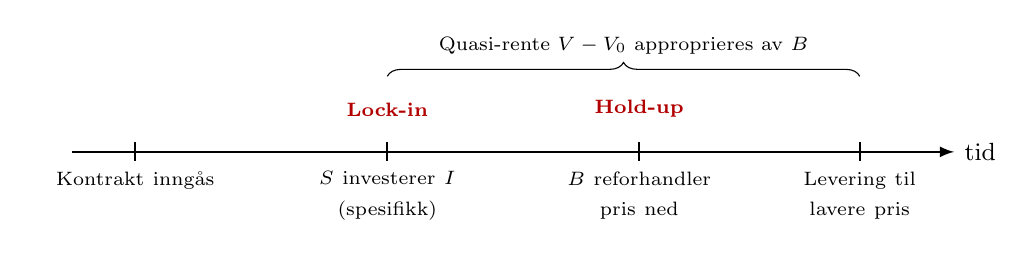
\begin{tikzpicture}[>=latex, scale=0.8, every node/.style={font=\small}]
  % Tidslinje
  \draw[->, thick] (0,0) -- (14,0) node[right] {tid};
  % Events
  \draw[thick] (1,0.15) -- (1,-0.15) node[below, text width=2.5cm, align=center] {\scriptsize Kontrakt inngås};
  \draw[thick] (5,0.15) -- (5,-0.15) node[below, text width=2.5cm, align=center] {\scriptsize $S$ investerer $I$\\(spesifikk)};
  \draw[thick] (9,0.15) -- (9,-0.15) node[below, text width=2.5cm, align=center] {\scriptsize $B$ reforhandler\\pris ned};
  \draw[thick] (12.5,0.15) -- (12.5,-0.15) node[below, text width=2.5cm, align=center] {\scriptsize Levering til\\lavere pris};
  % Labels above
  \node[above, red!70!black, font=\bfseries\scriptsize] at (5,0.4) {Lock-in};
  \node[above, red!70!black, font=\bfseries\scriptsize] at (9,0.4) {Hold-up};
  % Quasi-rent brace
  \draw[decorate, decoration={brace, amplitude=5pt}] (5,1.2) -- (12.5,1.2);
  \node[above] at (8.75,1.4) {\scriptsize Quasi-rente $V - V_0$ approprieres av $B$};
\end{tikzpicture}
\end{center}
\textit{Figur: Tidslinjen for hold-up. Etter spesifikk investering er $S$ locked in; $B$ utnytter dette ved reforhandling. [BOK]}

\subsection*{Eksempler}
\begin{itemize}\setlength{\itemsep}{2pt}
\item \textbf{GM--Fisher Body (1920-tallet):} Fisher Body investerte i pressverktøy spesifikt for GM-karosserier. Da etterspørselen steg, forsøkte Fisher å utnytte GMs avhengighet. GM løste hold-up ved å kjøpe Fisher Body (vertikal integrasjon). Klassisk eksempel i Williamson-litteraturen. [EKS]
\item \textbf{Intel og PC-produsenter:} Intel investerer lite relasjons\-spesifikt -- prosessorer er standardiserte. Lav asset specificity $\Rightarrow$ outsourcing fungerer. Kontrast til Fisher Body. [EKS]
\item \textbf{Mærsk og skipsverft (Hyundai Heavy):} Spesialdesignede containerskip representerer site-/physical-specificity. Mærsk sikrer seg med detaljerte kontrakter, milestone-betalinger og inspeksjonsrett -- kontraktuell safeguard i stedet for integrasjon. [CASE]
\end{itemize}

\subsection*{Kobling til søyle og andre teorier}
Søyle: \SOne\ (eierskap som allokering av residuell kontrollrett) og \SThree\ (insentiver til relasjonsspesifikk investering). Relaterte: \thref{vertical-integration-outsourcing}{Vertikal integrasjon og outsourcing}, \thref{boundaries-of-the-firm}{Boundaries of the Firm}, \thref{costly-contracting}{Costly contracting}, \thref{specific-vs-general-knowledge}{Spesifik vs.\ generell viden}, \thref{agency-costs}{Agency costs}.

\paragraph{Brukt i spørsmål:} Q12 (primært), Q11 (referert).

% !TEX root = ../main.tex
\section{Free-rider-problemet (nedstrøms)}\label{thr:free-rider-problem}

\paragraph{Definisjon.} I konteksten vertikal integrasjon vs.\ outsourcing oppstår \emph{free-rider-problemet} når uavhengige distributører underinvesterer i aktiviteter som gagner merket/produktet som helhet (service, markedsføring, showroom), fordi gevinsten av deres innsats deles med -- eller fanges av -- andre distributører. [SLIDE]

\subsection*{Forklaring}

BSZ kap.\ 19 diskuterer free-riding som et sentralt kontraktproblem ved outsourcet distribusjon. [SLIDE/BOK]

\textbf{Mekanisme:}
\begin{enumerate}\setlength{\itemsep}{2pt}
\item Produsent $P$ selger via uavhengige distributører $D_1, D_2, \ldots, D_n$.
\item Investering i kundeservice, showroom, rådgivning og lokal markedsføring er kostbart for den enkelte distributør.
\item Kunden bruker $D_1$s showroom for å teste produktet, men kjøper billigere fra $D_2$ som ikke investerer i service (\emph{inter-dealer free-riding}).
\item $D_1$s investering skaper en \emph{positiv eksternalitet} for $D_2$ -- en form for \thref{externalities}{eksternalitet} som markedet ikke internaliserer.
\item \emph{Resultat:} Alle distributører underinvesterer i service, merkevareverdi eroderes, og produsenten taper.
\end{enumerate}

\textbf{Varianter:}
\begin{itemize}\setlength{\itemsep}{1pt}
\item \textbf{Service free-riding:} Kunde bruker high-service dealer for rådgivning, kjøper fra discounter.
\item \textbf{Brand free-riding:} Distributør leverer dårlig service, men nyter godt av produsentens merkevare.
\item \textbf{Advertising free-riding:} Én distributørs reklamekampanje trekker kunder til regionen, men konkurrerende forhandlere fanger salget.
\end{itemize}

\textbf{Løsninger:}
\begin{itemize}\setlength{\itemsep}{2pt}
\item \textbf{Vertikal integrasjon} -- produsenten eier distributørkjeden og internaliserer eksternaliteten. [SLIDE]
\item \textbf{Resale price maintenance (RPM):} Minimumspris forhindrer priskutt som undergraver service-insentiv. Kontroversielt pga.\ konkurranserett. [BOK]
\item \textbf{Eksklusive territorier:} Hver distributør har monopol i sitt geografiske område -- inter-dealer free-riding elimineres. [BOK]
\item \textbf{Franchising med standardiserte servicekrav:} Franchisetaker forpliktes kontraktuelt til å investere i service (McDonald's, BMW). Brudd gir oppsigelse av kontrakt. [SLIDE]
\item \textbf{Produsenten finansierer:} Sentralisert markedsføring/service (co-op advertising) betalt av produsenten, fordelt via avgift. [BOK]
\end{itemize}

\subsection*{Kjerneforutsetninger}
\begin{itemize}
\item Distributørens serviceinvestering skaper verdi for kunder som kan kjøpe \emph{andre steder}.
\item Kunden kan separere informasjonsinnhenting fra kjøp (showrooming).
\item Distributørene er uavhengige profittmaksimerende enheter.
\item Produsenten kan ikke gratis observere eller kontrollere servicenivå (\thref{moral-hazard}{moral hazard}).
\end{itemize}

\subsection*{Muligheter}
\begin{itemize}
\item Forklarer franchising-modellens logikk: standardiserte kvalitetskrav + insentivsystem.
\item Forklarer eksklusive forhandleravtaler, minimumsannonsering og servicekrav i bilbransjen.
\item Forklarer hvorfor luksusmerker kontrollerer distribusjon strengere enn massemerker.
\end{itemize}

\subsection*{Begrensninger og kritikk}
\begin{itemize}
\item Internett har gjort showrooming massivt -- løsningene (RPM, eksklusive territorier) er stadig vanskeligere å håndheve.
\item RPM og eksklusive territorier kan være kartell-/monopolverktøy forkledd som anti-free-riding.
\item Franchising-kontrakten er selv kostbar å håndheve (\thref{costly-contracting}{costly contracting}).
\item Noen produkter trenger lite pre-sale service -- free-riding er da irrelevant, og outsourcing er uproblematisk.
\end{itemize}

\subsection*{Modell / illustrasjon}

\begin{figure}[H]
  \centering
  
\includegraphics[width=0.45\linewidth]{BSZ_kap_9_2026/by_slide/slide_015/BSZ_kap_9_2026_slide_015_asset_01_image4.jpeg}
  \caption{Free-rider-problemet i hverdagen: oppvasken ingen tar -- alle nyter godt av et rent kjøkken, men ingen vil bære kostnaden alene. (BSZ kap.\ 9, slide 15) [SLIDE]}
\end{figure}

\begin{center}
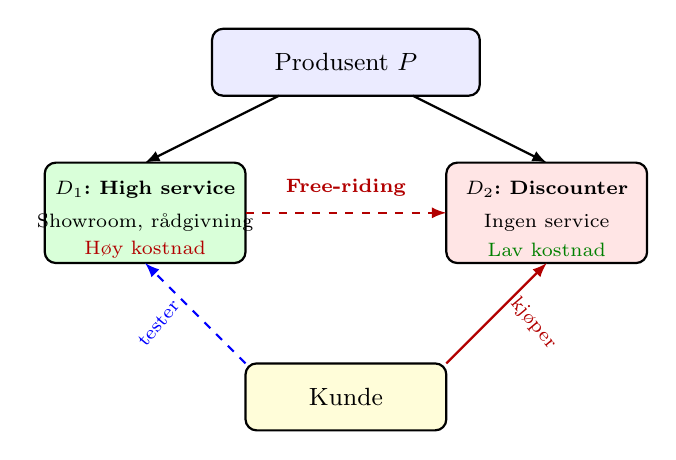
\begin{tikzpicture}[>=latex, scale=0.85, every node/.style={font=\small}]
  % Produsent
  \draw[thick, rounded corners, fill=blue!8] (3,5.5) rectangle (7,6.5);
  \node at (5,6.0) {Produsent $P$};
  % D1 high service
  \draw[thick, rounded corners, fill=green!15] (0.5,3.0) rectangle (3.5,4.5);
  \node[font=\bfseries\scriptsize] at (2,4.1) {$D_1$: High service};
  \node[font=\scriptsize] at (2,3.6) {Showroom, rådgivning};
  \node[font=\scriptsize, red!70!black] at (2,3.2) {Høy kostnad};
  % D2 discounter
  \draw[thick, rounded corners, fill=red!10] (6.5,3.0) rectangle (9.5,4.5);
  \node[font=\bfseries\scriptsize] at (8,4.1) {$D_2$: Discounter};
  \node[font=\scriptsize] at (8,3.6) {Ingen service};
  \node[font=\scriptsize, green!50!black] at (8,3.2) {Lav kostnad};
  % Arrows from P
  \draw[->, thick] (4,5.5) -- (2,4.5);
  \draw[->, thick] (6,5.5) -- (8,4.5);
  % Kunde
  \draw[thick, rounded corners, fill=yellow!15] (3.5,0.5) rectangle (6.5,1.5);
  \node at (5,1.0) {Kunde};
  % Kunde besøker D1, kjøper hos D2
  \draw[->, thick, dashed, blue] (3.5,1.5) -- (2,3.0);
  \node[font=\scriptsize, blue, rotate=50] at (2.2,2.1) {tester};
  \draw[->, thick, red!70!black] (6.5,1.5) -- (8,3.0);
  \node[font=\scriptsize, red!70!black, rotate=-50] at (7.8,2.1) {kjøper};
  % Free-rider label
  \draw[->, thick, red!70!black, dashed] (3.5,3.75) -- (6.5,3.75);
  \node[above, font=\scriptsize\bfseries, red!70!black] at (5,3.85) {Free-riding};
\end{tikzpicture}
\end{center}
\textit{Figur: Free-rider-problemet. Kunden tester hos high-service $D_1$ men kjøper hos discounter $D_2$. $D_2$ free-rider på $D_1$s service-investering. Begge distributører underinvesterer i likevekt. [BOK]}

\subsection*{Eksempler}
\begin{itemize}\setlength{\itemsep}{2pt}
\item \textbf{BMW og autoriserte forhandlere.} BMW krever at forhandlere investerer i showroom-standard, opplært personale og verkstedkvalitet. Uten disse kravene ville billige ``broker''-forhandlere free-ride på BMWs merkevare og autoriserte forhandleres serviceinvestering. Løsning: franchising med strenge standarder og eksklusive territorier. [EKS]
\item \textbf{Amazon vs.\ fysiske bokhandlere.} Bokhandlere med rådgivning og events investerer i leseropplevelse, men kunder scanner ISBN og bestiller billigere på Amazon (\emph{showrooming}). Klassisk free-riding -- har bidratt til nedleggelse av bokhandlere globalt. [EKS]
\item \textbf{Mærsk og agenter i utviklingsland.} Mærsk bruker egne kontorer i noen markeder (integrert) og uavhengige agenter i andre. Agenter kan underinvestere i Mærsk-spesifikk kundeservice fordi de også selger for konkurrenter -- free-riding på Mærsks merkenavn. [CASE]
\end{itemize}

\subsection*{Kobling til søyle og andre teorier}
Søyle: \SThree\ (insentivdesign for distributører) og \SOne\ (kontroll via eierskap eller kontraktsvilkår). Relaterte: \thref{vertical-integration-outsourcing}{Vertikal integrasjon og outsourcing}, \thref{externalities}{Eksternaliteter}, \thref{moral-hazard}{Moral hazard} (distributørens skjulte handling), \thref{costly-contracting}{Costly contracting}, \thref{residual-claimants}{Residual claimants}.

\paragraph{Brukt i spørsmål:} Q12 (primært), Q11 (referert).

% !TEX root = ../main.tex
\section{Double markup-problemet (dobbel marginalisering)}\label{thr:double-markup-problem}

\paragraph{Definisjon.} \emph{Double markup} (successive monopolies, dobbel marginalisering) oppstår når to suksessive monopolister -- en oppstrøms produsent og en nedstrøms distributør -- begge legger en markup over marginal kostnad. Resultatet er en sluttforbrukerpris som er \emph{høyere} og et kvantum som er \emph{lavere} enn det som maksimerer samlet verdikjedeprofitt. Vertikal integrasjon løser problemet ved å eliminere den ene markupen. [SLIDE]

\subsection*{Forklaring}

BSZ kap.\ 19 presenterer double markup som et uavhengig argument for vertikal integrasjon -- uavhengig av hold-up og free-riding. [SLIDE/BOK]

\textbf{Mekanisme (numerisk eksempel):}
\begin{enumerate}\setlength{\itemsep}{2pt}
\item Oppstrøms produsent $U$ har marginalkostnad $c=20$.
\item Nedstrøms distributør $D$ har kun distribusjonskostnad $=0$ for enkelhet.
\item Sluttetterspørsel: $P = 100 - Q$.
\item $U$ priser overfor $D$ som monopolist: $P_w = 60$ (halvveis mellom $c$ og chokeprisen).
\item $D$ tar $P_w=60$ som sin ``kostnad'' og priser overfor konsumenter som monopolist: $P_{\text{slutt}} = 80$.
\item \textbf{Kvantum $Q=20$, samlet profitt $= (80-20)\cdot 20 = 1{,}200$.}
\end{enumerate}

\textbf{Med vertikal integrasjon:}
\begin{enumerate}\setlength{\itemsep}{2pt}
\item Integrert firma priser direkte: $\max_{Q}\;(100-Q-20)\cdot Q \Rightarrow Q=40$, $P=60$.
\item \textbf{Kvantum $Q=40$, samlet profitt $= (60-20)\cdot 40 = 1{,}600$.}
\end{enumerate}

Integrasjon gir \emph{høyere} profitt (+33\%), \emph{lavere} sluttforbrukerpris (-25\%) og \emph{høyere} kvantum (+100\%). Alle parter (produsent, konsument) er bedre stilt -- \emph{alle vinner}. [BOK]

\textbf{Intuisjon:} Hver monopolist internaliserer ikke effekten av sin markup på den andres etterspørsel. To suksessive markups ``skatter'' etterspørselen to ganger -- en \emph{vertikal eksternalitet}. [SLIDE]

\subsection*{Kjerneforutsetninger}
\begin{itemize}
\item Begge ledd har markedsmakt (monopol eller dominant posisjon).
\item Kvantitet/pris i hvert ledd settes \emph{uavhengig} (Cournot/Stackelberg-struktur).
\item Ingen perfekt kontraktsløsning mellom $U$ og $D$ (ellers kunne man replisere integrasjonsutfallet med kontrakt).
\item Lineære priser (per-enhet wholesale price) -- med twopart tariff ($T + P_w \cdot Q$) kan $U$ ekstrahere surplus uten å vri pris, og double markup forsvinner.
\end{itemize}

\subsection*{Muligheter}
\begin{itemize}
\item Gir et \emph{effektivitetsargument} for vertikal integrasjon som selv konkurransemyndigheter aksepterer (lavere pris til forbruker).
\item Forklarer to-part-tariffer, RPM, franchise fees og andre mellomformer som løser problemet uten full integrasjon.
\item Predikerer at vertikale fusjoner i double-monopoly-industrier kan godkjennes av kartellmyndigheter.
\end{itemize}

\subsection*{Begrensninger og kritikk}
\begin{itemize}
\item Forutsetter markedsmakt i \emph{begge} ledd -- med konkurranse i nedstrøms (mange distributører) forsvinner $D$s markup, og problemet er irrelevant.
\item Two-part tariffer, franchise fees og RPM kan løse double markup kontraktuelt uten integrasjon.
\item Modellen ignorerer stordriftsfordeler, synergier og koordinasjonsgevinster som også motiverer integrasjon.
\item Statisk: ignorerer entry og dynamisk konkurranse.
\end{itemize}

\subsection*{Modell / illustrasjon}

\begin{figure}[H]
\centering
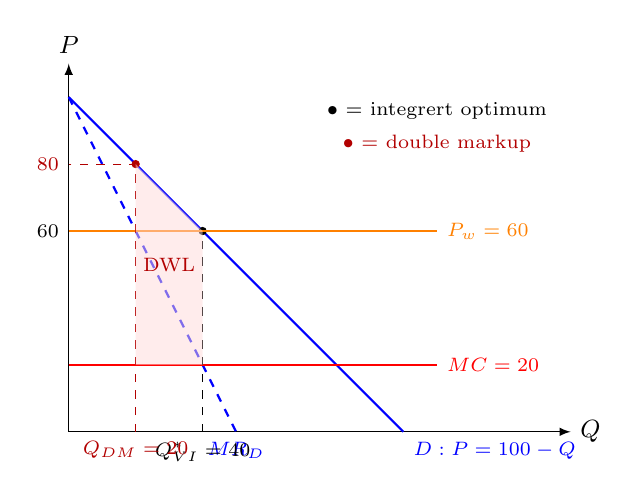
\begin{tikzpicture}[>=latex, scale=0.85, every node/.style={font=\small}]
  % Akser
  \draw[->] (0,0) -- (7.5,0) node[right] {$Q$};
  \draw[->] (0,0) -- (0,5.5) node[above] {$P$};
  % Etterspørsel P=100-Q skalert: P/20 og Q/10
  \draw[thick, blue] (0,5) -- (5,0) node[below right] {\scriptsize $D: P=100-Q$};
  % MR for etterspørsel
  \draw[thick, blue, dashed] (0,5) -- (2.5,0) node[below] {\scriptsize $MR_D$};
  % MC = 20 => 1.0 i skala
  \draw[thick, red] (0,1.0) -- (5.5,1.0) node[right] {\scriptsize $MC=20$};
  % Integrert optimum: Q=40, P=60
  \filldraw[black] (2.0,3.0) circle (1.5pt);
  \draw[dashed] (2.0,0) -- (2.0,3.0) -- (0,3.0);
  \node[below] at (2.0,0) {\scriptsize $Q^{*}_{VI}=40$};
  \node[left] at (0,3.0) {\scriptsize $60$};
  % Double markup: Pw=60, P_slutt=80, Q=20
  \draw[thick, orange] (0,3.0) -- (5.5,3.0) node[right] {\scriptsize $P_w=60$};
  % MR for D facing Pw=60: D's MR = 100-2Q, men D ser P_w som MC
  % D's optimum: MR_D = P_w => 100-2Q=60 => Q=20
  \filldraw[red!70!black] (1.0,4.0) circle (1.5pt);
  \draw[dashed, red!70!black] (1.0,0) -- (1.0,4.0) -- (0,4.0);
  \node[below, red!70!black] at (1.0,0) {\scriptsize $Q_{DM}=20$};
  \node[left, red!70!black] at (0,4.0) {\scriptsize $80$};
  % Shading dødvektstap
  \fill[red!15, opacity=0.5] (1.0,4.0) -- (2.0,3.0) -- (2.0,1.0) -- (1.0,1.0) -- cycle;
  \node[font=\scriptsize, red!70!black] at (1.5,2.5) {DWL};
  % Legend
  \node[font=\scriptsize] at (5.5,4.8) {$\bullet$ = integrert optimum};
  \node[font=\scriptsize, red!70!black] at (5.5,4.3) {$\bullet$ = double markup};
\end{tikzpicture}
\caption{\textbf{Double markup.} Med to uavhengige monopolister (oppstrøms og nedstrøms) ender sluttprisen på 80 med kvantum 20 (rødt punkt). Vertikal integrasjon gir $P=60$, $Q=40$ (svart punkt) -- lavere pris, høyere kvantum, eliminert dødvektstap (DWL). [BOK -- BSZ kap.\ 19]}
\end{figure}

\subsection*{Numerisk oppsummering}

\begin{center}
\renewcommand{\arraystretch}{1.15}
\begin{tabular}{@{}lccc@{}}
\toprule
 & \textbf{Double markup} & \textbf{Integrert} & \textbf{Endring} \\
\midrule
$P_{\text{slutt}}$ & 80 & 60 & $-25\%$ \\
$Q$ & 20 & 40 & $+100\%$ \\
Samlet profitt & 1{,}200 & 1{,}600 & $+33\%$ \\
Konsumentoverskudd & 200 & 800 & $+300\%$ \\
\bottomrule
\end{tabular}
\end{center}

\subsection*{Eksempler}
\begin{itemize}\setlength{\itemsep}{2pt}
\item \textbf{Farmasøytisk industri.} Legemiddelprodusent med patentmonopol selger til apotekkjeder med lokal markedsmakt. Begge legger markup -- pasienter betaler mer enn nødvendig. Løsning i Skandinavia: regulerte apotekpriser (RPM-variant) eller parallelimport. [EKS]
\item \textbf{Internettleverandører og innholdsleverandører.} ISP (monopolist i siste mil) og Netflix (dominant innhold) priset uavhengig -- double markup drev opp priser for forbrukere. Løst delvis via peering-avtaler og bundling. [EKS]
\end{itemize}

\subsection*{Kobling til søyle og andre teorier}
Søyle: \SOne\ (eierskap fjerner vertikal eksternalitet), \SThree\ (kontraktsdesign som alternativ til integrasjon). Relaterte: \thref{vertical-integration-outsourcing}{Vertikal integrasjon og outsourcing}, \thref{vertical-integration-market-power}{VI og market power}, \thref{externalities}{Eksternaliteter}, \thref{transfer-pricing}{Transfer pricing} (internpris kan settes til MC og eliminere dobbel markup).

\paragraph{Brukt i spørsmål:} Q12 (primært), Q11 (referert).

% Q13 theories
% !TEX root = ../main.tex
\section{Markedssvikt og regulering}\label{thr:market-failure-regulation}

\paragraph{Definisjon.} \emph{Offentlig indgriben} (regulering) er hensigtsmæssig når markedet selv ikke oppnår en effisient allokering -- dvs.\ ved \emph{markedssvikt}. De fire klassiske argumentene er: (1) naturlig monopol, (2) eksternaliteter, (3) offentlige goder, og (4) informasjonsasymmetri. Regulering søker å korrigere priser, kvantiteter eller atferd slik at utfallet nærmer seg det en perfekt-konkurranse-benchmark ville gitt. [SLIDE]

\subsection*{Forklaring}

BSZ kap.\ 21 presenterer fire forhold der markedet feiler og regulering kan forbedre utfallet: [SLIDE/BOK]

\textbf{1. Naturlig monopol.} Produksjon med fallende gjennomsnittskostnad (stordrift, høye faste kostnader, lave variable) gjør at én produsent er billigst -- men uten konkurranse setter monopolisten $P>MC$ og produserer for lite. Regulering: \emph{prisregulering} ($P=AC$ eller rate-of-return-regulering), konsesjonskrav, offentlig eierskap. Eksempler: strømnett, vannforsyning, jernbaneskinner. [SLIDE]

\textbf{2. Eksternaliteter.} Aktiviteter med positive eller negative konsekvenser for tredjepart som ikke prises av markedet. Se \thref{externalities}{eksternaliteter}. Negative eks.: forurensning (overproduksjon); positive eks.: utdanning, FoU (underproduksjon). Regulering: Pigou-skatt/subsidie, utslippskvoter, standarder. [SLIDE]

\textbf{3. Offentlige goder.} Goder som er \emph{ikke-rivaliserende} (min bruk reduserer ikke din) og \emph{ikke-ekskluderbare} (vanskelig å hindre gratispassasjerer). Free-riding gjør at markedet underproduserer. Regulering: offentlig tilbud, finansiering via skatt. Eksempler: forsvar, grunnforskning, fyrtårn. [BOK]

\textbf{4. Informasjonsasymmetri.} Selger vet mer om kvalitet enn kjøper (\thref{adverse-selection}{adverse selection}), eller aktør skjuler handling (\thref{moral-hazard}{moral hazard}). Markedet kan kollapse (Akerlof lemons). Regulering: obligatorisk informasjonsplikt (regnskap, prospekt), minstestandarder, sertifisering, forsikringskrav. [BOK]

\textbf{Forutsætninger for at regulering er hensigtsmæssig:}
\begin{itemize}\setlength{\itemsep}{1pt}
\item Markedssvikten er \emph{signifikant} -- reguleringsomkostningene må være lavere enn dødvektstapet.
\item Regulatoren har \emph{tilstrekkelig informasjon} til å sette korrekte priser/kvantiteter.
\item Reguleringsregimet er \emph{ikke kapert} av bransjen selv (regulatory capture).
\end{itemize}

\subsection*{Kjerneforutsetninger}
\begin{itemize}
\item Perfekt konkurranse er benchmark for effisient allokering.
\item Markedssvikt er kilden til problemet, ikke distribusjonspolitikk alene.
\item Regulatoren er (ideelt) benevolent og velinformert.
\item Regulering har selv kostnader (byråkrati, feilinformasjon, lobbying).
\end{itemize}

\subsection*{Muligheter}
\begin{itemize}
\item Gir normativt rammeverk for når staten bør gripe inn.
\item Forklarer regulering av energi, telekom, finans, helse, miljø.
\item Kobler til konkrete reguleringsverktøy: priskontroll, utslippskvoter, tilgangsregulering.
\end{itemize}

\subsection*{Begrensninger og kritikk}
\begin{itemize}
\item \textbf{Government failure:} Regulatoren kan mangle informasjon, være byråkratisk, eller bli korrumpert.
\item \textbf{Regulatory capture} (Stigler 1971): bransjen påvirker regulatoren til å sette regler som beskytter incumbents.
\item \textbf{Reguleringsarbitrasje:} Aktører tilpasser seg reguleringen uten å endre reell atferd.
\item \textbf{Dynamiske effekter:} Regulering kan hemme innovasjon og entry -- f.eks.\ rate-of-return-regulering gir Averch-Johnson-overinvestering i kapital.
\item \textbf{Public choice:} Politikere optimerer stemmer, ikke velferd -- regulering reflekterer politisk støtte-maksimering, ikke markedssvikt-korreksjon. Se \thref{regulated-pricing-model}{regulated pricing-modellen}.
\end{itemize}

\subsection*{Modell / illustrasjon}

\begin{figure}[H]
  \centering
  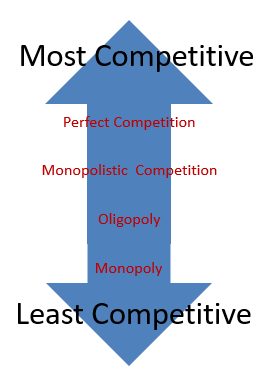
\includegraphics[width=0.35\linewidth]{BSZ_kap_6_2026/by_slide/slide_003/BSZ_kap_6_2026_slide_003_asset_01_image2.png}
  \caption{Markedsstrukturer fra perfekt konkurranse til monopol. Regulering griper inn der markedsmakt gir $P > MC$. (BSZ kap.\ 6, slide 3) [SLIDE]}
\end{figure}

\begin{center}
\renewcommand{\arraystretch}{1.15}
\begin{tabular}{@{}p{3.5cm}p{3.8cm}p{3.5cm}p{3.5cm}@{}}
\toprule
\textbf{Markedssvikt} & \textbf{Problem} & \textbf{Reguleringsverktøy} & \textbf{Eksempel} \\
\midrule
Naturlig monopol & $P>MC$, underproduksjon & Priskontroll, konsesjoner & Strømnett, vannverk \\
Eksternaliteter & Over-/underproduksjon & Pigou-skatt, kvoter & CO$_2$-avgift, ETS \\
Offentlige goder & Free-riding, under\-produksjon & Offentlig tilbud, skatt & Forsvar, FoU \\
Informasjonsasymmetri & Lemons, adverse selection & Informasjonsplikt, standarder & Regnskapskrav, FDA \\
\bottomrule
\end{tabular}
\end{center}
\textit{Tabell: De fire markedssviktene og korresponderende reguleringsverktøy. [SLIDE/BOK]}

\subsection*{Eksempler}
\begin{itemize}\setlength{\itemsep}{2pt}
\item \textbf{Norsk strømnett (Statnett):} Naturlig monopol regulert av NVE med inntektsramme-modell (rate-of-return-regulering). Sikrer lav pris men risikerer overinvestering (Averch-Johnson). [EKS]
\item \textbf{EU Emissions Trading System (ETS):} Regulering av CO$_2$-eksternalitet via kvotehandel -- Pigou-mekanisme. Prisen ($\sim$50--80 EUR/tonn) internaliserer deler av den negative eksternaliteten. [EKS]
\item \textbf{Mærsk Power-to-X og subsidier.} PtX mottar offentlig støtte fordi grønt hydrogen produserer positive eksternaliteter (klimareduksjon) som markedet underpriser. Subsidiering er reguleringsresponsen. [CASE]
\end{itemize}

\subsection*{Kobling til søyle og andre teorier}
Søyle: \SOne\ (regulatoren allokerer beslutningsrettigheter mellom stat og marked). Relaterte: \thref{externalities}{Eksternaliteter}, \thref{adverse-selection}{Adverse selection}, \thref{moral-hazard}{Moral hazard}, \thref{regulated-pricing-model}{Regulated pricing-modellen}, \thref{vertical-integration-market-power}{VI og market power}.

\paragraph{Brukt i spørsmål:} Q13.

% !TEX root = ../main.tex
\section{Regulated pricing-modellen (branche-profit og political support)}\label{thr:regulated-pricing-model}

\paragraph{Definisjon.} BSZ kap.\ 21 presenterer en modell der regulerte priser bestemmes som et kompromiss mellom \emph{brancheprofitt} $\pi(P)$ og \emph{political support} $S(\pi, CS)$. Regulatoren (politikeren) maksimerer ikke velferd direkte, men velger den prisen som maksimerer politisk støtte -- en funksjon av både produsentprofitt og konsumentoverskudd. [SLIDE]

\subsection*{Forklaring}

Modellen bygger på public choice-tradisjonen (Peltzman 1976, Stigler 1971) og forklarer hvorfor regulerte priser typisk er \emph{mellom} monopolpris og marginal\-kostnadspris. [SLIDE/BOK]

\textbf{Byggeklossene:}

\textbf{1. Branche-profit-funksjonen $\pi(P)$.} Bransjens profitt som funksjon av regulert pris $P$:
\begin{itemize}\setlength{\itemsep}{1pt}
\item $\pi(P)$ er null ved $P=AC$ (break-even) og stigende med $P$ opp til monopolpris $P^M$.
\item $\pi(P^M)$ er maksimal profitt; over $P^M$ faller etterspørsel og profitt.
\item Formen er invers-U: $\pi(P)$ stiger fra $P=AC$, topper ved $P^M$, synker deretter.
\end{itemize}

\textbf{2. Konsumentoverskudd $CS(P)$.} Konsumentoverskudd er fallende i $P$: høyere pris $\Rightarrow$ lavere CS.

\textbf{3. Political support-funksjonen $S(\pi, CS)$.} Politikeren vinner støtte fra to grupper:
\begin{itemize}\setlength{\itemsep}{1pt}
\item \textbf{Bransjen/industrien:} lobbyer, kampanjebidrag, arbeidsplasser $\Rightarrow$ støtte stiger i $\pi$.
\item \textbf{Konsumenter/velgere:} stemmer, offentlig opinion $\Rightarrow$ støtte stiger i $CS$.
\item $S$ er stigende i begge, men med avtagende marginaleffekt: $\partial S/\partial \pi > 0$, $\partial S/\partial CS > 0$, $\partial^2 S/\partial \pi^2 < 0$, $\partial^2 S/\partial CS^2 < 0$.
\end{itemize}

\textbf{4. Regulatorens valg.} Regulatoren velger $P^{*}$ som maksimerer $S(\pi(P), CS(P))$:
\[
\frac{dS}{dP} = \frac{\partial S}{\partial \pi}\cdot\pi'(P) + \frac{\partial S}{\partial CS}\cdot CS'(P) = 0
\]
Førsteordensbetingelsen sier at marginal politisk gevinst fra økt brancheprofitt (ved å heve $P$) lik marginal politisk kostnad fra redusert konsumentoverskudd. [BOK]

\textbf{Resultat:} $P^{*}$ ligger mellom $P^{MC}$ (marginal\-kostnadspris, ren konsumentoptimal) og $P^{M}$ (monopolpris, ren bransjeoptimal). Den eksakte plasseringen avhenger av de relative vektene $\partial S/\partial \pi$ vs.\ $\partial S/\partial CS$ -- altså bransjens vs.\ konsumentenes politiske innflytelse.

\subsection*{Grafisk modell -- political support-optimering}

\begin{figure}[h]
\centering
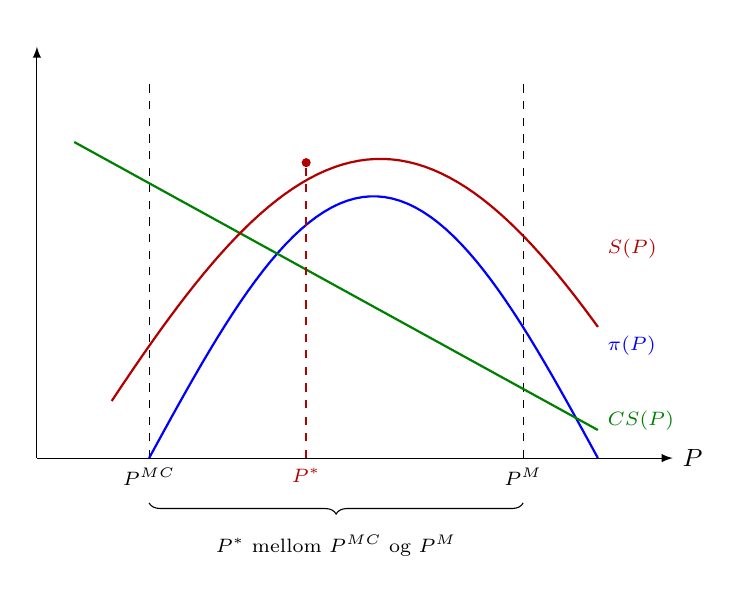
\begin{tikzpicture}[>=latex, scale=0.95, every node/.style={font=\small}]
  % Akser
  \draw[->] (0,0) -- (8.5,0) node[right] {$P$};
  \draw[->] (0,0) -- (0,5.5) node[above] {};
  % MC-pris og monopolpris
  \draw[dashed] (1.5,0) -- (1.5,5.0);
  \node[below] at (1.5,0) {\scriptsize $P^{MC}$};
  \draw[dashed] (6.5,0) -- (6.5,5.0);
  \node[below] at (6.5,0) {\scriptsize $P^{M}$};
  % Profit function pi(P) -- invers U
  \draw[thick, blue, domain=1.5:7.5, samples=60]
    plot (\x, {3.5*sin((\x-1.5)*30)});
  \node[blue, right] at (7.5,1.5) {\scriptsize $\pi(P)$};
  % CS(P) -- fallende
  \draw[thick, green!50!black, domain=0.5:7.5, samples=40]
    plot (\x, {4.5-0.55*\x});
  \node[green!50!black, right] at (7.5,0.5) {\scriptsize $CS(P)$};
  % S(P) -- invers U men toppen forskjøvet til venstre for pi-toppen
  \draw[thick, red!70!black, domain=1.0:7.5, samples=60]
    plot (\x, {4.0*sin((\x-0.5)*22)});
  \node[red!70!black, right] at (7.5,2.8) {\scriptsize $S(P)$};
  % P* optimum
  \draw[thick, dashed, red!70!black] (3.6,0) -- (3.6,4.0);
  \node[below, red!70!black, font=\bfseries] at (3.6,0) {\scriptsize $P^{*}$};
  \filldraw[red!70!black] (3.6,3.95) circle (1.5pt);
  % Brace
  \draw[decorate, decoration={brace, amplitude=4pt, mirror}] (1.5,-0.6) -- (6.5,-0.6);
  \node[below, font=\scriptsize] at (4.0,-0.9) {$P^{*}$ mellom $P^{MC}$ og $P^{M}$};
\end{tikzpicture}
\caption{\textbf{Regulated pricing-modellen.} Brancheprofitt $\pi(P)$ (blå) er invers-U med topp ved monopolpris $P^M$. Konsumentoverskudd $CS(P)$ (grønn) er fallende. Political support $S(P)$ (rød) balanserer de to og topper ved $P^*$ -- mellom $P^{MC}$ og $P^M$. Regulatoren velger $P^*$ der marginal politisk gevinst fra bransjen lik marginal politisk kostnad fra konsumenter. [BOK -- BSZ kap.\ 21]}
\end{figure}

\subsection*{Komparativ statikk}
\begin{itemize}\setlength{\itemsep}{2pt}
\item \textbf{Sterkere bransjelobby} ($\partial S/\partial \pi$ øker): $P^{*}$ skifter mot $P^M$. Eks.: regulerte monopoler med sterk industriorganisasjon.
\item \textbf{Sterkere konsumentpress} ($\partial S/\partial CS$ øker): $P^{*}$ skifter mot $P^{MC}$. Eks.: medieoppmerksomhet, forbrukerorganisasjoner.
\item \textbf{Mer elastisk etterspørsel:} $\pi(P)$ flater ut raskere -- $P^M$ senkes og dermed $P^{*}$.
\end{itemize}

\subsection*{Kjerneforutsetninger}
\begin{itemize}
\item Regulatoren er en rasjonell politisk aktør som maksimerer støtte, ikke velferd.
\item Bransjen og konsumenter konkurrerer om politisk innflytelse via lobbying, stemmer og kampanjebidrag.
\item $S$ er en konkav funksjon av $\pi$ og $CS$ separat (avtagende marginalnytte av begge).
\item Prisen er det eneste reguleringsverktøyet (forenklet).
\end{itemize}

\subsection*{Muligheter}
\begin{itemize}
\item Forklarer hvorfor regulerte priser sjelden er ren MC-prising (for lav profitt gir bransjeprotest) eller ren monopolpris (for lavt CS gir velgerprotest).
\item Predikerer reguleringsutfall som funksjon av relative lobbyingsressurser.
\item Forklarer regulatory capture: når $\partial S/\partial \pi \gg \partial S/\partial CS$, settes $P^{*}\approx P^M$.
\item Forklarer variasjoner i regulering mellom bransjer og land.
\end{itemize}

\subsection*{Begrensninger og kritikk}
\begin{itemize}
\item Reduserer regulering til ren maktkamp -- ignorerer faglige avveininger og juridiske rammer.
\item Forutsetter at regulatoren har full informasjon om $\pi(P)$ og $CS(P)$ -- i praksis strategisk informasjonsasymmetri fra bransjen.
\item Modellen er statisk; reguleringsregimer utvikles over tid med nye aktører, teknologi og politikk.
\item Forutsetter én regulert pris -- i praksis er regulering multidimensjonell (pris, kvalitet, tilgang, investeringskrav).
\item Konsumenter er ofte dårlig organisert (Olsons kollektiv handling-problem) -- modellen undervurderer systematisk bransjens overvekt.
\end{itemize}

\subsection*{Eksempler}
\begin{itemize}\setlength{\itemsep}{2pt}
\item \textbf{Norsk farmasiregulering.} Statens legemiddelverk setter maksimale apotekpriser som balanserer farmasøytisk bransjeprofitt (innovasjonsinsentiv) mot pasientenes betalingsevne. Resultatet: priser lavere enn USA (svakt bransjepress) men høyere enn generiske alternativer (bransjens lobbying mot tvangs-generisk substitusjon). [EKS]
\item \textbf{Norsk taxi-regulering (pre-2020).} Løyvemonopol ga sjåfører monopolprofitt men høye priser. Politisk støtte fra organisertetaxisjåfører (sterk lobby) vs.\ diffuse konsumenter. Deregulering i 2020 skiftet $P^{*}$ nedover etter økt konsumentpress (Uber-debatt). [EKS]
\end{itemize}

\subsection*{Kobling til søyle og andre teorier}
Søyle: \SOne\ (regulatoren allokerer beslutningsrettigheter mellom stat og marked). Relaterte: \thref{market-failure-regulation}{Markedssvikt og regulering}, \thref{externalities}{Eksternaliteter}, \thref{vertical-integration-market-power}{VI og market power}, \thref{principal-agent}{Principal-agent} (regulatoren som agent for velgere).

\paragraph{Brukt i spørsmål:} Q13.

% Q14 theories
% !TEX root = ../main.tex
\section{Informativeness-prinsippet}\label{thr:informativeness-principle}

\paragraph{Definisjon.} \emph{Informativeness-prinsippet} (Holmström 1979) sier at et ekstra signal $y$ bør inkluderes i kontrakten hvis og bare hvis det er \emph{statistisk informativt om agentens innsats} $e$ -- dvs.\ at observasjon av $y$ endrer posterior-sannsynligheten for $e$ gitt det primære prestasjonsmålet $Q$. Formelt: $y$ er informativt $\Leftrightarrow$ $f(Q,y|e)$ avhenger av $e$ på en måte som ikke allerede fanges av $Q$ alene. [SLIDE]

\subsection*{Forklaring}

BSZ kap.\ 15 bruker informativeness-prinsippet til å forklare hvorfor kontrakter ofte inkluderer flere måltall, og til å binde sammen (a) kontrollerbarhet, (b) risikodeling, (c) målingers presisjon og (d) risikopremie. [SLIDE/BOK]

\textbf{Kjernelogikk.} I den lineære principal-agent-modellen ($W=W_0+\beta Q$, $Q=\alpha e+\mu$) avhenger den optimale insentivkoeffisienten \thref{incentive-coefficient}{$\beta^*$} av signal-støy-forholdet. Informativeness-prinsippet generaliserer dette: [BOK]

\begin{enumerate}\setlength{\itemsep}{2pt}
\item \textbf{Tilleggssignal $y$.} Anta at et ekstra observerbart signal $y$ er tilgjengelig (f.eks.\ bransjeavkastning, peer-gruppers prestasjon, kundetilfredshet, input-mål).
\item \textbf{Statistisk test.} $y$ er informativt om $e$ $\Leftrightarrow$ fordelingen $f(Q|e,y) \neq f(Q|e)$ for noen $(Q,y)$. Intuitivt: $y$ ``filtrerer bort'' støy fra $Q$ og gjør det lettere å slutte seg til $e$.
\item \textbf{Kontraktuell konsekvens.} Hvis $y$ er informativt, skal optimal kontrakt betinge kompensasjon på \emph{både} $Q$ og $y$: $W = W_0 + \beta_1 Q + \beta_2 y$. Dette \emph{reduserer den effektive støyen} agenten bærer, og tillater høyere $\beta_1$ (sterkere insentiv) uten å øke risikopremien.
\item \textbf{Sufficient statistics.} Omvendt: hvis $Q$ er en \emph{sufficient statistic} for $e$ (all informasjon om $e$ allerede finnes i $Q$), skal $y$ \emph{ikke} inkluderes -- det tilfører bare støy uten innsatsinformasjon.
\end{enumerate}

\textbf{Kobling til de fire delspørsmålene:}

\textbf{(a) Kontrollerbarhet.} \thref{controllability-principle}{Controllability-prinsippet} sier at agenten kun skal måles på det hun kontrollerer. Informativeness-prinsippet \emph{generaliserer} dette: et ukontrollerbart mål kan likevel inkluderes i kontrakten hvis det er informativt om innsats. Eksempel: bransjeavkastning (peer-gruppe) er ikke kontrollerbar av agenten, men er informativ fordi den filtrerer felles markedssjokk fra agentens individuelle prestasjon. [SLIDE]

\textbf{(b) Risikodeling.} Jo mer informative signalene er, desto mer presist kan innsats estimeres, og desto \emph{lavere} risikopremie trenger prinsipalen å betale. Informativeness forbedrer \thref{risk-sharing}{risikodelingen} uten å svekke insentivene. Se formelen: risikopremie $\approx \tfrac{r}{2}\beta^2\sigma^2_{\text{eff}}$ -- informativeness senker $\sigma^2_{\text{eff}}$. [BOK]

\textbf{(c) Målingers presisjon.} Et prestasjonsmål med lav varians $\sigma^2$ er et mer presist signal om innsats. Informativeness-prinsippet predikerer at presise mål bør vektes høyere i kontrakten ($\beta$ høyere), og upresise mål lavere. Mer presise mål $\Rightarrow$ høyere $\beta^*$ $\Rightarrow$ sterkere insentiver $\Rightarrow$ lavere agency costs. [SLIDE]

\textbf{(d) Risikopremie.} Risikopremien $RP = \tfrac{r}{2}\beta^2\sigma^2$ er den direkte kostnaden av å bruke et støyfullt mål som kontraktsgrunnlag. Informativeness-prinsippet sier: legg til signaler som senker effektiv $\sigma^2$, og unngå signaler som bare tilfører støy. Resultatet er lavere $RP$ for gitt insentivnivå. [BOK]

\subsection*{Kjerneforutsetninger}
\begin{itemize}
\item Agentens innsats $e$ er ikke direkte observerbar (\thref{moral-hazard}{moral hazard}).
\item Signaler er kostnadsfritt tilgjengelige (ellers må informasjonsverdien veies mot innsamlingskostnaden).
\item Lineær kontrakt (i generelle modeller gjelder prinsippet mer bredt).
\item Prinsipalen forplikter seg til kontrakten ex ante -- ingen renegotiation.
\end{itemize}

\subsection*{Muligheter}
\begin{itemize}
\item Forklarer hvorfor kontrakter bruker \thref{absolute-vs-relative-performance}{relative prestasjonsmål} (peer-grupper filtrerer felles sjokk).
\item Forklarer indekserte aksjeopsjoner (fjerner markedsbevegelsen, isolerer firmaspesifikk avkastning).
\item Forklarer balansert målekort: flere indikatorer som sammen gir et mer informativt bilde av innsats.
\item Gir normativt kriterium: inkludér et mål $\Leftrightarrow$ det er informativt om innsats.
\item Utvider controllability: ukontrollerbare mål kan likevel være verdifulle.
\end{itemize}

\subsection*{Begrensninger og kritikk}
\begin{itemize}
\item Flere signaler øker kontraktskompleksitet -- agenten forstår kanskje ikke eget insentivsystem (kognitiv overbelastning).
\item Modellen antar at signaler er gratis tilgjengelige -- i praksis koster informasjonsinnsamling.
\item Holmström--Milgrom (1991) multitasking: mer informative mål på én dimensjon kan \emph{vri} innsats bort fra umålbare dimensjoner.
\item Empirisk: vanskelig å teste prinsippet direkte fordi optimal kontraktsdesign er uobserverbar.
\item Forutsetter at regulatoren/prinsipalen kan prosessere mange signaler uten bias -- i praksis brukes tommelfingerregler.
\end{itemize}

\subsection*{Modell / illustrasjon}

\begin{figure}[h]
\centering
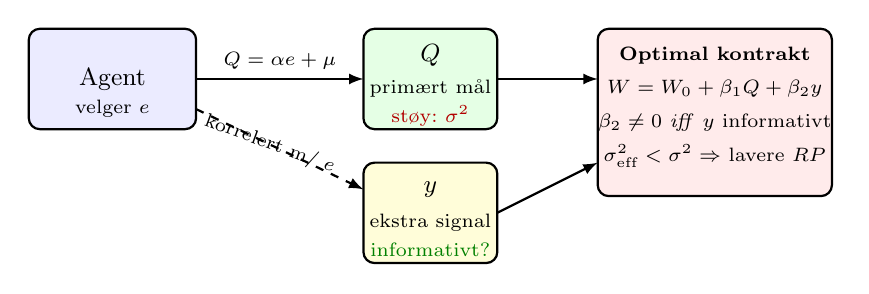
\begin{tikzpicture}[>=latex, scale=0.85, every node/.style={font=\small}]
  % Agent
  \draw[thick, rounded corners, fill=blue!8] (0,2.5) rectangle (2.5,4.0);
  \node at (1.25,3.25) {Agent};
  \node[font=\scriptsize] at (1.25,2.8) {velger $e$};
  % Output Q
  \draw[->, thick] (2.5,3.25) -- (5.0,3.25);
  \node[above, font=\scriptsize] at (3.75,3.25) {$Q = \alpha e + \mu$};
  % Q box
  \draw[thick, rounded corners, fill=green!10] (5.0,2.5) rectangle (7.0,4.0);
  \node at (6.0,3.6) {$Q$};
  \node[font=\scriptsize] at (6.0,3.1) {primært mål};
  \node[font=\scriptsize, red!70!black] at (6.0,2.7) {støy: $\sigma^2$};
  % Extra signal y
  \draw[thick, rounded corners, fill=yellow!15] (5.0,0.5) rectangle (7.0,2.0);
  \node at (6.0,1.6) {$y$};
  \node[font=\scriptsize] at (6.0,1.1) {ekstra signal};
  \node[font=\scriptsize, green!50!black] at (6.0,0.7) {informativt?};
  % Arrow from agent to y
  \draw[->, thick, dashed] (2.5,2.8) -- (5.0,1.6);
  \node[above, font=\scriptsize, rotate=-20] at (3.5,2.0) {korrelert m/ $e$};
  % Contract box
  \draw[thick, rounded corners, fill=red!8] (8.5,1.5) rectangle (12.0,4.0);
  \node[font=\bfseries\scriptsize] at (10.25,3.6) {Optimal kontrakt};
  \node[font=\scriptsize] at (10.25,3.1) {$W = W_0 + \beta_1 Q + \beta_2 y$};
  \node[font=\scriptsize] at (10.25,2.6) {$\beta_2 \neq 0$ \emph{iff} $y$ informativt};
  \node[font=\scriptsize] at (10.25,2.1) {$\sigma^2_{\text{eff}} < \sigma^2 \Rightarrow$ lavere $RP$};
  % Arrows to contract
  \draw[->, thick] (7.0,3.25) -- (8.5,3.25);
  \draw[->, thick] (7.0,1.25) -- (8.5,2.0);
\end{tikzpicture}
\caption{\textbf{Informativeness-prinsippet.} Agenten velger innsats $e$, som påvirker primærmål $Q$ (med støy $\sigma^2$). Et tilleggssignal $y$ inkluderes i kontrakten \emph{bare} hvis det er informativt om $e$ -- altså endrer den statistiske inferensen om $e$ gitt $Q$. Resultat: lavere effektiv støy $\sigma^2_{\text{eff}}$, lavere risikopremie, sterkere insentiver mulig. [SLIDE/BOK]}
\end{figure}

\subsection*{Eksempler}
\begin{itemize}\setlength{\itemsep}{2pt}
\item \textbf{Relative aksjeavkastningsmål (rTSR).} CEO-bonus baseres ikke bare på egen aksjekurs ($Q$) men relativt til peer-gruppe ($y$). Peer-avkastning er informativ om markedssjokk, ikke om CEOs innsats -- ved å trekke fra fjernes felles støy. Informativeness-prinsippet er det teoretiske grunnlaget for rTSR-programmer. [EKS]
\item \textbf{Oljebransjen og oljeprisen.} Oljeprisen er ikke kontrollerbar for Equinor-CEO, men er informativ: den filtrerer ut eksogent prissjokk fra firmaspesifikk prestasjon. Bonus justert for oljepris (eller bransjejustert) bruker informativeness-prinsippet. [EKS]
\item \textbf{Balansert målekort (Kaplan \& Norton).} Finansielle + operasjonelle + kunde + læringsmål: hvert mål tilfører informasjon om dimensjoner av innsats som finansmålet alene ikke fanger -- informativeness-prinsippet begrunner multi-dimensjonell måling. [EKS]
\end{itemize}

\subsection*{Kobling til søyle og andre teorier}
Søyle: \STwo\ (hvilke mål å inkludere) og \SThree\ (kontraktsdesign og $\beta$-valg). Relaterte: \thref{controllability-principle}{Controllability-prinsippet}, \thref{incentive-coefficient}{Incentive coefficient}, \thref{risk-sharing}{Risk sharing}, \thref{optimal-effort-model}{Optimal effort-modell}, \thref{principal-agent}{Principal-agent}, \thref{moral-hazard}{Moral hazard}, \thref{absolute-vs-relative-performance}{Absolutt vs.\ relativ prestasjonsmåling}, \thref{fixed-vs-variable-pay}{Fast vs.\ variabel lønn}, \thref{agency-costs}{Agency costs}.

\paragraph{Brukt i spørsmål:} Q14 (primært), Q09 (referert), Q10 (referert).

% Q15 theories
% !TEX root = ../main.tex
\section{Integrity vs.\ Income-modellen}\label{thr:integrity-vs-income-model}

\paragraph{Definisjon.} BSZ kap.\ 2 presenterer en nyttemodell der medarbeideren velger mellom to ``goder'': \emph{integritet} (etisk atferd, regeloverholdelse) og \emph{indkomst} (personlig inntekt/bonus). Kompensasjonsplanens design endrer budsjettbetingelsen og dermed agentens optimale valg -- selv for en agent som verdsetter integritet, kan et dårlig designet insentivsystem vippe valget mot uetisk atferd. [SLIDE]

\subsection*{Forklaring}

Modellen bruker standard mikroøkonomisk rammeverk (indifferenskurver + budsjettlinje) overført til et ikke-standard godsrom: integritet og indkomst. [SLIDE/BOK]

\textbf{Akser:}
\begin{itemize}\setlength{\itemsep}{1pt}
\item \textbf{Horisontal:} Integritet (fra lav til høy; mer integritet = mer regeloverholdelse, mindre juks).
\item \textbf{Vertikal:} Indkomst (personlig inntekt/bonus).
\end{itemize}

\textbf{Indifferenskurver:} Agenten har preferanser over begge goder. Indifferenskurvene er konvekse mot origo: agenten er villig til å bytte noe integritet mot mer inntekt (og omvendt). MRS mellom indkomst og integritet varierer -- noen verdsetter integritet høyt (bratte kurver), andre lavt (flate kurver). [BOK]

\textbf{Budsjettlinje (opportunity set):} Kompensasjonsplanen definerer hvilke kombinasjoner av integritet og indkomst som er tilgjengelige:
\begin{itemize}\setlength{\itemsep}{2pt}
\item \textbf{Før aggressivt insentivsystem:} Budsjettlinjen er relativt flat -- inntektsforskjellen mellom ``jukse'' og ``ikke jukse'' er liten. Agenten velger høy integritet.
\item \textbf{Etter aggressivt insentivsystem:} Budsjettlinjen roterer utover -- inntektsgevinsten ved å jukse (fire kunder, ta snarveier, falske salg) øker dramatisk. Agenten kan nå oppnå mye høyere inntekt ved å ofre integritet.
\item \textbf{Resultat:} Tangentpunktet mellom indifferenskurve og budsjettlinje skifter mot lavere integritet og høyere inntekt.
\end{itemize}

\textbf{Nøkkelinnsikt:} Kompensasjonsdesign er ikke bare et spørsmål om å ``motivere innsats'' -- det påvirker \emph{hva slags} innsats som velges. En kontrakt med høy $\beta$ på enkelt målbare resultater (salg, antall kontoer) uten sjekk på kvalitet/etikk dreier agenten bort fra integritet. [SLIDE]

\subsection*{Grafisk modell}

\begin{figure}[H]
  \centering
  
\includegraphics[width=0.35\linewidth]{BSZ_kap_2_2026/by_slide/slide_005/BSZ_kap_2_2026_slide_005_asset_01_image4.png}
  \caption{Metafor: pengeankret drar agenten ned. Et aggressivt insentivsystem øker den personlige kostnaden ved å forbli etisk -- selv en agent som verdsetter integritet, kan dras mot uetisk atferd når relativprisen mellom integritet og inntekt endres tilstrekkelig. (BSZ kap.\ 2, slide 5) [SLIDE]}
\end{figure}

\begin{figure}[H]
\centering
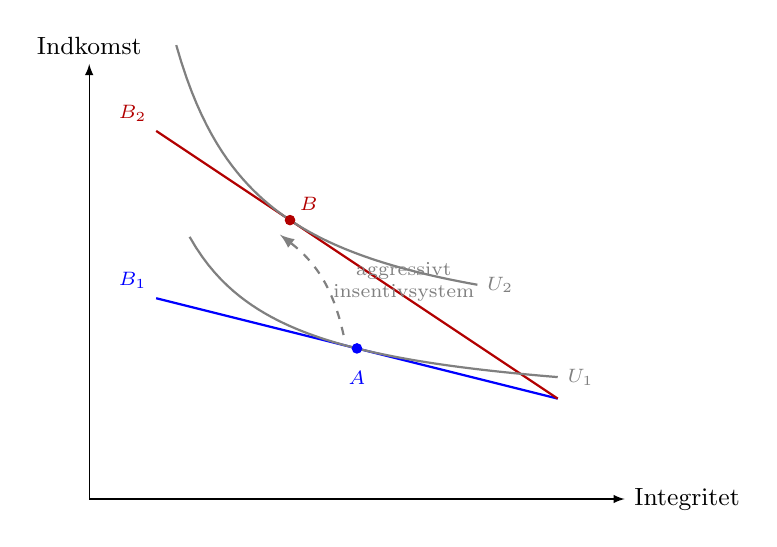
\begin{tikzpicture}[>=latex, scale=0.85, every node/.style={font=\small}]
  % Akser
  \draw[->] (0,0) -- (8,0) node[right] {Integritet};
  \draw[->] (0,0) -- (0,6.5) node[above] {Indkomst};
  % Budsjettlinje 1 (moderat insentiv)
  \draw[thick, blue] (1.0,3.0) -- (7.0,1.5);
  \node[blue, above left, font=\scriptsize] at (1.0,3.0) {$B_1$};
  % Budsjettlinje 2 (aggressivt insentiv - rotert)
  \draw[thick, red!70!black] (1.0,5.5) -- (7.0,1.5);
  \node[red!70!black, above left, font=\scriptsize] at (1.0,5.5) {$B_2$};
  % Indifferenskurve U1: y = 4/x + 1.25, tangent til B1 i (4, 2.25)
  \draw[thick, gray, domain=1.5:7.0, samples=60]
    plot (\x, {4/\x + 1.25});
  \node[gray, right, font=\scriptsize] at (7.0,1.82) {$U_1$};
  % Indifferenskurve U2: y = 6/x + 13/6, tangent til B2 i (3, 25/6)
  \draw[thick, gray, domain=1.3:5.8, samples=60]
    plot (\x, {6/\x + 13/6});
  \node[gray, right, font=\scriptsize] at (5.8,3.20) {$U_2$};
  % Tangent A (høy integritet, B1) ved (4, 2.25)
  \filldraw[blue] (4.0,2.25) circle (2pt);
  \node[below, blue, font=\bfseries\scriptsize] at (4.0,2.05) {$A$};
  % Tangent B (lav integritet, B2) ved (3, 25/6 ~ 4.167)
  \filldraw[red!70!black] (3.0,4.167) circle (2pt);
  \node[above right, red!70!black, font=\bfseries\scriptsize] at (3.0,4.167) {$B$};
  % Annotations
  \draw[->, thick, dashed, gray] (3.8,2.45) to[bend right=20] (2.85,3.95);
  \node[font=\scriptsize, gray, text width=2.5cm, align=center] at (4.7,3.25) {aggressivt\\insentiv\-system};
\end{tikzpicture}
\caption{\textbf{Integrity vs.\ Income.} Med moderat insentiv (blå $B_1$) velger agenten punkt $A$: høy integritet, moderat inntekt. Etter innføring av aggressivt prestasjonsbasert insentiv (rød $B_2$) roterer budsjettlinjen utover -- gevinsten ved å ofre integritet øker. Nytt optimum er punkt $B$: lav integritet, høy inntekt. Kompensasjonsdesignet endrer etisk atferd uten å endre preferanser. [SLIDE -- BSZ kap.\ 2]}
\end{figure}

\subsection*{Kjerneforutsetninger}
\begin{itemize}
\item Agenten har stabile preferanser som inkluderer integritet som et gode (ikke bare inntekt).
\item Kompensasjonsplanen endrer relativprisen mellom integritet og inntekt.
\item Integritet er \emph{ikke} perfekt overvåkbart -- ellers kunne prinsipalen kontraktfeste etikk direkte.
\item Standard nytteteori: konvekse indifferenskurver, monotone preferanser.
\end{itemize}

\subsection*{Muligheter}
\begin{itemize}
\item Forklarer corporate scandals som resultat av insentivsystem, ikke bare ``dårlige mennesker''.
\item Gir normativt verktøy: design kompensasjonsplaner som \emph{ikke} gjør det irrasjonelt å være etisk.
\item Viser at etikk og insentiver er komplementære designvariabler -- begge hører til den organisatoriske arkitekturen.
\item Kobler insentivdesign (\SThree) til kultur og governance.
\end{itemize}

\subsection*{Begrensninger og kritikk}
\begin{itemize}
\item ``Integritet'' som målbart gode er en sterk abstraksjon -- etiske valg er ofte binære (jukse/ikke jukse), ikke kontinuerlige.
\item Modellen ignorerer sosiale normer, gruppepress og culture som påvirker atferd uavhengig av insentiver.
\item Forutsetter rasjonelt valg -- atferdsøkonomi viser at etiske valg ofte er intuitive, ikke kalkulerte.
\item Alternativ forklaring: insentiver kan \emph{crowde ut} indre motivasjon (Frey \& Jegen 2001) -- noe modellen ikke fanger.
\end{itemize}

\subsection*{Eksempler}
\begin{itemize}\setlength{\itemsep}{2pt}
\item \textbf{Wells Fargo (2016):} Aggressive cross-sell-kvoter roterte budsjettlinjen kraftig -- bankansatte valgte punkt $B$: 3{,}5 mill.\ falske kontoer. Etter skandalen reduserte Wells Fargo $\beta$ og innførte kvalitative mål -- budsjettlinjen roterte tilbake. [EKS]
\item \textbf{Enron (2001):} Mark-to-market-basert bonus ga enormt insentiv til å oppblåse verdier. Ansatte med ellers god integritet justerte estimater aggressivt fordi budsjettlinjen premiertete det. [EKS]
\item \textbf{Skandinaviske banker etter hvitvaskingsskandalene (Danske Bank, Swedbank):} Compliance-kultur styrket og bonusandelen redusert -- budsjettlinjen rotert tilbake mot integritet. [EKS]
\end{itemize}

\subsection*{Kobling til søyle og andre teorier}
Søyle: \SThree\ (kompensasjonsdesign påvirker etisk atferd), \STwo\ (hva som måles bestemmer hva som belønnes). Relaterte: \thref{incentive-coefficient}{Incentive coefficient} ($\beta$ driver rotasjonen), \thref{moral-hazard}{Moral hazard}, \thref{principal-agent}{Principal-agent}, \thref{gaming-in-performance-measurement}{Gaming} (integrity--income-trade-offen er en form for gaming), \thref{risk-expected-value-model}{Risk--expected value-modellen} (den andre nyttemodellen i Q15).

\paragraph{Brukt i spørsmål:} Q15.

% !TEX root = ../main.tex
\section{Risk--Expected Value-modellen (indifferenskurver i $(\sigma, E[W])$-rommet)}\label{thr:risk-expected-value-model}

\paragraph{Definisjon.} BSZ kap.\ 2/15 presenterer en modell der medarbeideren velger mellom kontrakter som gir ulike kombinasjoner av \emph{risiko} ($\sigma$ eller $\sigma^2$, variansen i kompensasjon) og \emph{forventet verdi} ($E[W]$, forventet lønn). Agentens preferanser representeres av indifferenskurver i $(\sigma, E[W])$-rommet, der risikoaversjon bestemmer kurvenes helning: en risikoavers agent krever høyere $E[W]$ for å akseptere mer risiko (\emph{risikopremie}). [SLIDE]

\subsection*{Forklaring}

Modellen kobler sammen \thref{risk-sharing}{risikodeling}, \thref{reservation-utility}{reservation utility} og \thref{incentive-coefficient}{incentive coefficient} i ett grafisk rammeverk. [SLIDE/BOK]

\textbf{Akser:}
\begin{itemize}\setlength{\itemsep}{1pt}
\item \textbf{Horisontal:} Risiko -- standardavviket (eller variansen) i kompensasjon, $\sigma_W = \beta\sigma$.
\item \textbf{Vertikal:} Forventet verdi -- $E[W] = W_0 + \beta\alpha e^*$.
\end{itemize}

\textbf{Indifferenskurver:} Gitt CARA-nytte ($U = E[W] - \tfrac{r}{2}\mathrm{Var}[W]$) er indifferenskurvene \emph{stigende} og \emph{konvekse oppover} i $(\sigma^2, E[W])$-rommet:
\[
E[W] = \bar{U} + \tfrac{r}{2}\sigma_W^2
\]
Hvert nyttenivå $\bar{U}$ gir en oppovervåkende parabel. Risikoaversjon $r$ bestemmer helningen: høyere $r$ $\Rightarrow$ brattere kurver $\Rightarrow$ agenten krever mer kompensasjon for ekstra risiko. [BOK]

\textbf{Nøkkelkonsepter:}
\begin{itemize}\setlength{\itemsep}{2pt}
\item \textbf{Certainty equivalent (CE):} Skjæringspunktet mellom indifferenskurven og vertikalaksen ($\sigma=0$). Det sikre beløpet agenten er indifferent mellom og det usikre alternativet.
\item \textbf{Risikopremie (RP):} $RP = E[W] - CE = \tfrac{r}{2}\beta^2\sigma^2$. Avstanden mellom forventet verdi og certainty equivalent.
\item \textbf{Risikonøytral agent ($r=0$):} Indifferenskurvene er horisontale -- agenten bryr seg bare om $E[W]$.
\item \textbf{Svært risikoavers agent ($r$ stor):} Bratte indifferenskurver -- krever stor $E[W]$-økning for litt mer risiko.
\end{itemize}

\textbf{Kobling til kontraktsdesign:} Når prinsipalen tilbyr en kontrakt med bestemt $\beta$, bestemmer dette en linje i $(\sigma, E[W])$-rommet. Agenten aksepterer kontrakten bare hvis den tilbudte kombinasjonen når minst \thref{reservation-utility}{reservation utility} ($\bar{U} \geq U_0$). Optimal kontrakt er det punktet på denne linjen som tangerer agentens reservation-indifferenskurve. [SLIDE]

\subsection*{Grafisk modell}

\begin{figure}[h]
\centering
\begin{tikzpicture}[>=latex, scale=0.85, every node/.style={font=\small}]
  % Akser
  \draw[->] (0,0) -- (8,0) node[right] {$\sigma_W$ (risiko)};
  \draw[->] (0,0) -- (0,7) node[above] {$E[W]$};
  % Indifferenskurver risikoavers (r stor)
  \draw[thick, blue, domain=0:5.5, samples=40]
    plot (\x, {1.5 + 0.15*\x*\x});
  \node[blue, right, font=\scriptsize] at (5.5,6.0) {$U_0$ (risikoavers)};
  \draw[thick, blue, dashed, domain=0:5.0, samples=40]
    plot (\x, {2.5 + 0.15*\x*\x});
  \node[blue, right, font=\scriptsize] at (5.0,6.3) {$U_1 > U_0$};
  % Indifferenskurver risikonøytral
  \draw[thick, green!50!black, domain=0:7.0, samples=20]
    plot (\x, {3.0});
  \node[green!50!black, right, font=\scriptsize] at (7.0,3.0) {risikonøytral};
  % CE og RP
  \draw[dashed] (0,1.5) -- (3.5,1.5);
  \node[left, font=\scriptsize] at (0,1.5) {$CE$};
  \filldraw[blue] (3.5, 3.34) circle (1.5pt);
  \node[above left, font=\scriptsize\bfseries, blue] at (3.5,3.34) {$A$};
  \draw[dashed] (3.5,0) -- (3.5,3.34);
  \draw[dashed] (0,3.34) -- (3.5,3.34);
  \node[left, font=\scriptsize] at (0,3.34) {$E[W]_A$};
  % RP brace
  \draw[decorate, decoration={brace, amplitude=4pt, mirror}, red!70!black] (-0.3,1.5) -- (-0.3,3.34);
  \node[left, font=\scriptsize, red!70!black] at (-0.6,2.42) {$RP$};
  % Point annotation
  \node[below, font=\scriptsize] at (3.5,0) {$\sigma_A$};
\end{tikzpicture}
\caption{\textbf{Risk--Expected Value.} Indifferenskurver i $(\sigma_W, E[W])$-rommet. Risikoavers agent (blå): stigende, konvekse kurver -- krever høyere $E[W]$ for mer risiko. Punkt $A$: en kontrakt med risiko $\sigma_A$ krever forventet lønn $E[W]_A$; agentens certainty equivalent er $CE$ (skjæring med $y$-aksen). Risikopremien $RP = E[W]_A - CE$ er prinsiplens kostnad. Risikonøytral agent (grønn): flat kurve -- ingen risikopremie nødvendig. [SLIDE -- BSZ kap.\ 2/15]}
\end{figure}

\subsection*{Kjerneforutsetninger}
\begin{itemize}
\item CARA-nytte (konstant absolutt risikoaversjon) for at indifferenskurvene er parallelle.
\item Risiko representert ved $\sigma_W$ eller $\sigma^2_W$ -- normalfordelt avkastning.
\item Agenten har \thref{reservation-utility}{reservation utility} $U_0$ som sett av markedet.
\item Prinsipalen er risikonøytral (diversifisert aksjonær).
\end{itemize}

\subsection*{Muligheter}
\begin{itemize}
\item Visualiserer risikopremien og certainty equivalent grafisk -- intuitivt for eksamen.
\item Forklarer hvorfor risikoaverse agenter krever høyere forventet lønn for å akseptere variabel kompensasjon.
\item Kobler direkte til $\beta^*$-formelen: høyere $\beta$ $\Rightarrow$ beveger agenten nordøst langs budsjettlinjen $\Rightarrow$ mer risiko, mer $E[W]$, men stigende $RP$.
\item Viser forskjell mellom risikoavers, risikonøytral og risikosøkende agent visuelt.
\end{itemize}

\subsection*{Begrensninger og kritikk}
\begin{itemize}
\item CARA-nytte er en sterk forutsetning -- i virkeligheten er risikoaversjon avhengig av formue (DARA er mer realistisk).
\item Modellen ignorerer loss aversion (Kahneman \& Tversky): nedsiderisiko vektes tyngre enn oppside.
\item Normalfordeling forutsetter symmetrisk risiko -- i praksis er kompensasjon ofte asymmetrisk (opsjoner har begrenset nedside).
\item Grafisk representasjon fungerer for to dimensjoner -- med flere risikofaktorer kreves mer formalisering.
\end{itemize}

\subsection*{Eksempler}
\begin{itemize}\setlength{\itemsep}{2pt}
\item \textbf{Nyutdannet konsulent vs.\ erfaren partner.} Konsulenten (lav formue, høy $r$) har bratte indifferenskurver og velger fastlønn. Partneren (høy formue, diversifisert, lav $r$) har flate kurver og aksepterer profittpoolbonus. Samme firma, ulik kontrakt -- forklart av forskjell i indifferenskurve-helning. [EKS]
\item \textbf{Equinor-ansatte og aksjespareprogram.} Equinor tilbyr aksjer med rabatt -- ansatte velger ulik andel avhengig av risikoaversjon. Risikoaverse (ingeniører med høy gjeld) velger lite, risikotolerante (eldre uten boliggjeld) velger mye. Modellen forklarer seleksjonsmønsteret. [EKS]
\end{itemize}

\subsection*{Kobling til søyle og andre teorier}
Søyle: \SThree\ (kompensasjonsdesign bestemmer agentens risiko-avkastnings-profil). Relaterte: \thref{risk-sharing}{Risk sharing}, \thref{reservation-utility}{Reservation utility}, \thref{incentive-coefficient}{Incentive coefficient}, \thref{fixed-vs-variable-pay}{Fast vs.\ variabel lønn}, \thref{optimal-effort-model}{Optimal effort-modell}, \thref{integrity-vs-income-model}{Integrity vs.\ income-modellen} (den andre nyttemodellen i Q15).

\paragraph{Brukt i spørsmål:} Q15.


\end{document}
